%**************************************%
%* Generated from MathBook XML source *%
%*    on 2017-03-20T15:02:00-07:00    *%
%*                                    *%
%*   http://mathbook.pugetsound.edu   *%
%*                                    *%
%**************************************%
\documentclass[10pt,]{book}
%% Custom Preamble Entries, early (use latex.preamble.early)
%% Inline math delimiters, \(, \), need to be robust
%% 2016-01-31:  latexrelease.sty  supersedes  fixltx2e.sty
%% If  latexrelease.sty  exists, bugfix is in kernel
%% If not, bugfix is in  fixltx2e.sty
%% See:  https://tug.org/TUGboat/tb36-3/tb114ltnews22.pdf
%% and read "Fewer fragile commands" in distribution's  latexchanges.pdf
\IfFileExists{latexrelease.sty}{}{\usepackage{fixltx2e}}
%% Text height identically 9 inches, text width varies on point size
%% See Bringhurst 2.1.1 on measure for recommendations
%% 75 characters per line (count spaces, punctuation) is target
%% which is the upper limit of Bringhurst's recommendations
%% Load geometry package to allow page margin adjustments
\usepackage{geometry}
\geometry{letterpaper,total={340pt,9.0in}}
%% Custom Page Layout Adjustments (use latex.geometry)
%% This LaTeX file may be compiled with pdflatex, xelatex, or lualatex
%% The following provides engine-specific capabilities
%% Generally, xelatex and lualatex will do better languages other than US English
%% You can pick from the conditional if you will only ever use one engine
\usepackage{ifthen}
\usepackage{ifxetex,ifluatex}
\ifthenelse{\boolean{xetex} \or \boolean{luatex}}{%
%% begin: xelatex and lualatex-specific configuration
%% fontspec package will make Latin Modern (lmodern) the default font
\ifxetex\usepackage{xltxtra}\fi
\usepackage{fontspec}
%% realscripts is the only part of xltxtra relevant to lualatex 
\ifluatex\usepackage{realscripts}\fi
%% 
%% Extensive support for other languages
\usepackage{polyglossia}
\setdefaultlanguage{english}
%% Magyar (Hungarian)
\setotherlanguage{magyar}
%% Spanish
\setotherlanguage{spanish}
%% Vietnamese
\setotherlanguage{vietnamese}
%% end: xelatex and lualatex-specific configuration
}{%
%% begin: pdflatex-specific configuration
%% translate common Unicode to their LaTeX equivalents
%% Also, fontenc with T1 makes CM-Super the default font
%% (\input{ix-utf8enc.dfu} from the "inputenx" package is possible addition (broken?)
\usepackage[T1]{fontenc}
\usepackage[utf8]{inputenc}
%% end: pdflatex-specific configuration
}
%% Monospace font: Inconsolata (zi4)
%% Sponsored by TUG: http://levien.com/type/myfonts/inconsolata.html
%% See package documentation for excellent instructions
%% One caveat, seem to need full file name to locate OTF files
%% Loads the "upquote" package as needed, so we don't have to
%% Upright quotes might come from the  textcomp  package, which we also use
%% We employ the shapely \ell to match Google Font version
%% pdflatex: "varqu" option produces best upright quotes
%% xelatex,lualatex: add StylisticSet 1 for shapely \ell
%% xelatex,lualatex: add StylisticSet 2 for plain zero
%% xelatex,lualatex: we add StylisticSet 3 for upright quotes
%% 
\ifthenelse{\boolean{xetex} \or \boolean{luatex}}{%
%% begin: xelatex and lualatex-specific monospace font
\usepackage{zi4}
\setmonofont[BoldFont=Inconsolatazi4-Bold.otf,StylisticSet={1,3}]{Inconsolatazi4-Regular.otf}
%% end: xelatex and lualatex-specific monospace font
}{%
%% begin: pdflatex-specific monospace font
\usepackage[varqu]{zi4}
%% end: pdflatex-specific monospace font
}
%% Symbols, align environment, bracket-matrix
\usepackage{amsmath}
\usepackage{amssymb}
%% allow page breaks within display mathematics anywhere
%% level 4 is maximally permissive
%% this is exactly the opposite of AMSmath package philosophy
%% there are per-display, and per-equation options to control this
%% split, aligned, gathered, and alignedat are not affected
\allowdisplaybreaks[4]
%% allow more columns to a matrix
%% can make this even bigger by overriding with  latex.preamble.late  processing option
\setcounter{MaxMatrixCols}{30}
%%
%% Color support, xcolor package
%% Always loaded.  Used for:
%% mdframed boxes, add/delete text, author tools
\PassOptionsToPackage{usenames,dvipsnames,svgnames,table}{xcolor}
\usepackage{xcolor}
%%
%% Semantic Macros
%% To preserve meaning in a LaTeX file
%% Only defined here if required in this document
%% Used for inline definitions of terms
\newcommand{\terminology}[1]{\textbf{#1}}
%% Used for fillin answer blank
%% Argument is length in em
\newcommand{\fillin}[1]{\underline{\hspace{#1em}}}
%% Subdivision Numbering, Chapters, Sections, Subsections, etc
%% Subdivision numbers may be turned off at some level ("depth")
%% A section *always* has depth 1, contrary to us counting from the document root
%% The latex default is 3.  If a larger number is present here, then
%% removing this command may make some cross-references ambiguous
%% The precursor variable $numbering-maxlevel is checked for consistency in the common XSL file
\setcounter{secnumdepth}{3}
%% mdframed environments use a tikz frame method
\usepackage{tikz}%% Environments with amsthm package
%% Theorem-like environments in "plain" style, with or without proof
\usepackage{amsthm}
\theoremstyle{plain}
%% Numbering for Theorems, Conjectures, Examples, Figures, etc
%% Controlled by  numbering.theorems.level  processing parameter
%% Always need a theorem environment to set base numbering scheme
%% even if document has no theorems (but has other environments)
\newtheorem{theorem}{Theorem}[chapter]
%% Only variants actually used in document appear here
%% Style is like a theorem, and for statements without proofs
%% Numbering: all theorem-like numbered consecutively
%% i.e. Corollary 4.3 follows Theorem 4.2
%% Remark-like environments, normal text
%% Numbering is in sync with theorems, etc
\theoremstyle{definition}
\newtheorem{remark}[theorem]{Remark}
\newtheorem{warning}[theorem]{Caution}
%% Example-like environments, normal text
%% Numbering is in sync with theorems, etc
\theoremstyle{definition}
\newtheorem{example}[theorem]{Example}
%% Package for breakable highlight boxes
\usepackage[framemethod=tikz]{mdframed}
%% begin: assemblage
%% minimally structured content, high visibility presentation
%% environments (untitled, titled), with style
\newenvironment{assemblage-untitled}{\mdfsetup{%
roundcorner=2ex, backgroundcolor=blue!5,linecolor=blue!75!black,}%
\begin{mdframed}}{\end{mdframed}}
\newenvironment{assemblage}[1]{\mdfsetup{frametitle={\colorbox{blue!20}{\space#1\space}},%
frametitlealignment={\hspace*{1ex}}, frametitleaboveskip=-1.5ex, frametitlebelowskip=0pt,%
roundcorner=2ex, backgroundcolor=blue!5,linecolor=blue!75!black,}%
\begin{mdframed}}{\end{mdframed}}
%% end: assemblage
%% Miscellaneous environments, normal text
%% Numbering for inline exercises and lists is in sync with theorems, etc
\theoremstyle{definition}
\newtheorem{exercise}[theorem]{Exercise}
%% Localize LaTeX supplied names (possibly none)
\renewcommand*{\appendixname}{Appendix}
\renewcommand*{\chaptername}{Chapter}
%% Equation Numbering
%% Controlled by  numbering.equations.level  processing parameter
\numberwithin{equation}{part}
%% For improved tables
\usepackage{array}
%% Some extra height on each row is desirable, especially with horizontal rules
%% Increment determined experimentally
\setlength{\extrarowheight}{0.2ex}
%% Define variable thickness horizontal rules, full and partial
%% Thicknesses are 0.03, 0.05, 0.08 in the  booktabs  package
\makeatletter
\newcommand{\hrulethin}  {\noalign{\hrule height 0.04em}}
\newcommand{\hrulemedium}{\noalign{\hrule height 0.07em}}
\newcommand{\hrulethick} {\noalign{\hrule height 0.11em}}
%% We preserve a copy of the \setlength package before other
%% packages (extpfeil) get a chance to load packages that redefine it
\let\oldsetlength\setlength
\newlength{\Oldarrayrulewidth}
\newcommand{\crulethin}[1]%
{\noalign{\global\oldsetlength{\Oldarrayrulewidth}{\arrayrulewidth}}%
\noalign{\global\oldsetlength{\arrayrulewidth}{0.04em}}\cline{#1}%
\noalign{\global\oldsetlength{\arrayrulewidth}{\Oldarrayrulewidth}}}%
\newcommand{\crulemedium}[1]%
{\noalign{\global\oldsetlength{\Oldarrayrulewidth}{\arrayrulewidth}}%
\noalign{\global\oldsetlength{\arrayrulewidth}{0.07em}}\cline{#1}%
\noalign{\global\oldsetlength{\arrayrulewidth}{\Oldarrayrulewidth}}}
\newcommand{\crulethick}[1]%
{\noalign{\global\oldsetlength{\Oldarrayrulewidth}{\arrayrulewidth}}%
\noalign{\global\oldsetlength{\arrayrulewidth}{0.11em}}\cline{#1}%
\noalign{\global\oldsetlength{\arrayrulewidth}{\Oldarrayrulewidth}}}
%% Single letter column specifiers defined via array package
\newcolumntype{A}{!{\vrule width 0.04em}}
\newcolumntype{B}{!{\vrule width 0.07em}}
\newcolumntype{C}{!{\vrule width 0.11em}}
\makeatother
%% Figures, Tables, Listings, Floats
%% The [H]ere option of the float package fixes floats in-place,
%% in deference to web usage, where floats are totally irrelevant
%% We re/define the figure, table and listing environments, if used
%%   1) New mbxfigure and/or mbxtable environments are defined with float package
%%   2) Standard LaTeX environments redefined to use new environments
%%   3) Standard LaTeX environments redefined to step theorem counter
%%   4) Counter for new environments is set to the theorem counter before caption
%% You can remove all this figure/table setup, to restore standard LaTeX behavior
%% HOWEVER, numbering of figures/tables AND theorems/examples/remarks, etc
%% WILL ALL de-synchronize with the numbering in the HTML version
%% You can remove the [H] argument of the \newfloat command, to allow flotation and 
%% preserve numbering, BUT the numbering may then appear "out-of-order"
\usepackage{float}
\usepackage[bf]{caption} % http://tex.stackexchange.com/questions/95631/defining-a-new-type-of-floating-environment 
\usepackage{newfloat}
% Figure environment setup so that it no longer floats
\SetupFloatingEnvironment{figure}{fileext=lof,placement={H},within=chapter,name=Figure}
% figures have the same number as theorems: http://tex.stackexchange.com/questions/16195/how-to-make-equations-figures-and-theorems-use-the-same-numbering-scheme 
\makeatletter
\let\c@figure\c@theorem
\makeatother
% Table environment setup so that it no longer floats
\SetupFloatingEnvironment{table}{fileext=lot,placement={H},within=chapter,name=Table}
% tables have the same number as theorems: http://tex.stackexchange.com/questions/16195/how-to-make-equations-figures-and-theorems-use-the-same-numbering-scheme 
\makeatletter
\let\c@table\c@theorem
\makeatother
%% Musical Symbol Support
\ifthenelse{\boolean{xetex}}{
%% begin: xelatex-specific configuration
\usepackage{lilyglyphs}
\lilyGlobalOptions{scale=0.8}
\newcommand*{\doubleflat}{\flatflat}
%% end: xelatex-specific configuration
}{
%% begin: pdflatex-specific configuration
\DeclareFontFamily{U}{musix}{}%
\DeclareFontShape{U}{musix}{m}{n}{%
<-12>   musix11
<12-15> musix13
<15-18> musix16
<18-23> musix20
<23->   musix29
}{}%
%% We grab all five accidentals from the musix font so they are usable in both math and text mode
\renewcommand*\flat{\raisebox{0.5ex}{\usefont{U}{musix}{m}{n}\selectfont{2}}}
\newcommand*\doubleflat{\raisebox{0.5ex}{\usefont{U}{musix}{m}{n}\selectfont{3}}}
\renewcommand*\sharp{\raisebox{0.5ex}{\usefont{U}{musix}{m}{n}\selectfont{4}}}
\newcommand*\doublesharp{\raisebox{0.5ex}{\usefont{U}{musix}{m}{n}\selectfont{5}}}
\renewcommand*\natural{\raisebox{0.5ex}{\usefont{U}{musix}{m}{n}\selectfont{6}}}
%% end: pdflatex-specific configuration
}
%% Raster graphics inclusion, wrapped figures in paragraphs
%% \resizebox sometimes used for images in side-by-side layout
\usepackage{graphicx}
%%
%% Program listing support, for inline code, Sage code
\usepackage{listings}
%% We define the listings font style to be the default "ttfamily"
%% To fix hyphens/dashes rendered in PDF as fancy minus signs by listing
%% http://tex.stackexchange.com/questions/33185/listings-package-changes-hyphens-to-minus-signs
\makeatletter
\lst@CCPutMacro\lst@ProcessOther {"2D}{\lst@ttfamily{-{}}{-{}}}
\@empty\z@\@empty
\makeatother
\ifthenelse{\boolean{xetex}}{}{%
%% begin: pdflatex-specific listings configuration
%% translate U+0080 - U+00F0 to their textmode LaTeX equivalents
%% Data originally from https://www.w3.org/Math/characters/unicode.xml, 2016-07-23
%% Lines marked in XSL with "$" were converted from mathmode to textmode
\lstset{extendedchars=true}
\lstset{literate={ }{{~}}{1}{¡}{{\textexclamdown }}{1}{¢}{{\textcent }}{1}{£}{{\textsterling }}{1}{¤}{{\textcurrency }}{1}{¥}{{\textyen }}{1}{¦}{{\textbrokenbar }}{1}{§}{{\textsection }}{1}{¨}{{\textasciidieresis }}{1}{©}{{\textcopyright }}{1}{ª}{{\textordfeminine }}{1}{«}{{\guillemotleft }}{1}{¬}{{\textlnot }}{1}{­}{{\-}}{1}{®}{{\textregistered }}{1}{¯}{{\textasciimacron }}{1}{°}{{\textdegree }}{1}{±}{{\textpm }}{1}{²}{{\texttwosuperior }}{1}{³}{{\textthreesuperior }}{1}{´}{{\textasciiacute }}{1}{µ}{{\textmu }}{1}{¶}{{\textparagraph }}{1}{·}{{\textperiodcentered }}{1}{¸}{{\c{}}}{1}{¹}{{\textonesuperior }}{1}{º}{{\textordmasculine }}{1}{»}{{\guillemotright }}{1}{¼}{{\textonequarter }}{1}{½}{{\textonehalf }}{1}{¾}{{\textthreequarters }}{1}{¿}{{\textquestiondown }}{1}{À}{{\`{A}}}{1}{Á}{{\'{A}}}{1}{Â}{{\^{A}}}{1}{Ã}{{\~{A}}}{1}{Ä}{{\"{A}}}{1}{Å}{{\AA }}{1}{Æ}{{\AE }}{1}{Ç}{{\c{C}}}{1}{È}{{\`{E}}}{1}{É}{{\'{E}}}{1}{Ê}{{\^{E}}}{1}{Ë}{{\"{E}}}{1}{Ì}{{\`{I}}}{1}{Í}{{\'{I}}}{1}{Î}{{\^{I}}}{1}{Ï}{{\"{I}}}{1}{Ð}{{\DH }}{1}{Ñ}{{\~{N}}}{1}{Ò}{{\`{O}}}{1}{Ó}{{\'{O}}}{1}{Ô}{{\^{O}}}{1}{Õ}{{\~{O}}}{1}{Ö}{{\"{O}}}{1}{×}{{\texttimes }}{1}{Ø}{{\O }}{1}{Ù}{{\`{U}}}{1}{Ú}{{\'{U}}}{1}{Û}{{\^{U}}}{1}{Ü}{{\"{U}}}{1}{Ý}{{\'{Y}}}{1}{Þ}{{\TH }}{1}{ß}{{\ss }}{1}{à}{{\`{a}}}{1}{á}{{\'{a}}}{1}{â}{{\^{a}}}{1}{ã}{{\~{a}}}{1}{ä}{{\"{a}}}{1}{å}{{\aa }}{1}{æ}{{\ae }}{1}{ç}{{\c{c}}}{1}{è}{{\`{e}}}{1}{é}{{\'{e}}}{1}{ê}{{\^{e}}}{1}{ë}{{\"{e}}}{1}{ì}{{\`{\i}}}{1}{í}{{\'{\i}}}{1}{î}{{\^{\i}}}{1}{ï}{{\"{\i}}}{1}{ð}{{\dh }}{1}{ñ}{{\~{n}}}{1}{ò}{{\`{o}}}{1}{ó}{{\'{o}}}{1}{ô}{{\^{o}}}{1}{õ}{{\~{o}}}{1}{ö}{{\"{o}}}{1}{÷}{{\textdiv }}{1}{ø}{{\o }}{1}{ù}{{\`{u}}}{1}{ú}{{\'{u}}}{1}{û}{{\^{u}}}{1}{ü}{{\"{u}}}{1}{ý}{{\'{y}}}{1}{þ}{{\th }}{1}{ÿ}{{\"{y}}}{1}}
%% end: pdflatex-specific listings configuration
}
%% End of generic listing adjustments
%% Inline code, typically from "c" element
%% Global, document-wide options apply to \lstinline
%% Search/replace \lstinline by \verb to remove this dependency
%% (redefining \lstinline with \verb is unlikely to work)
%% Also see "\renewcommand\UrlFont" below for matching font choice
\lstset{basicstyle=\small\ttfamily,breaklines=true,breakatwhitespace=true,extendedchars=true,inputencoding=latin1}
%% Multiple column, column-major lists
\usepackage{multicol}
%% More flexible list management, esp. for references and exercises
%% But also for specifying labels (i.e. custom order) on nested lists
\usepackage{enumitem}
%% Lists of references in their own section, maximum depth 1
\newlist{referencelist}{description}{4}
\setlist[referencelist]{leftmargin=!,labelwidth=!,labelsep=0ex,itemsep=1.0ex,topsep=1.0ex,partopsep=0pt,parsep=0pt}
%% Lists of exercises in their own section, maximum depth 4
\newlist{exerciselist}{description}{4}
\setlist[exerciselist]{leftmargin=0pt,itemsep=1.0ex,topsep=1.0ex,partopsep=0pt,parsep=0pt}
%% Indented groups of exercises within an exercise section
%% Add  debug=true  option to see boxes around contents
\usepackage{tasks}
\NewTasks[label-format=\bfseries,item-indent=3.3em,label-offset=0.4em,label-width=1.7em,label-align=right,after-item-skip=\smallskipamount,after-skip=\smallskipamount]{exercisegroup}[\exercise]
%% Support for index creation
%% imakeidx package does not require extra pass (as with makeidx)
%% Title of the "Index" section set via a keyword
%% Language support for the "see" and "see also" phrases
\usepackage{imakeidx}
\makeindex[title=Index, intoc=true]
\renewcommand{\seename}{see}
\renewcommand{\alsoname}{see also}
%% hyperref driver does not need to be specified
\usepackage{hyperref}
%% Hyperlinking active in PDFs, all links solid and blue
\hypersetup{colorlinks=true,linkcolor=blue,citecolor=blue,filecolor=blue,urlcolor=blue}
\hypersetup{pdftitle={Test chapter}}
%% If you manually remove hyperref, leave in this next command
\providecommand\phantomsection{}
%% Graphics Preamble Entries
\usepackage{stackengine}
\usepackage{cancel}
\usepackage{xcolor}
\renewcommand{\CancelColor}{blue}
%% If tikz has been loaded, replace ampersand with \amp macro
%% NB: calc redefines \setlength
\usepackage{calc}
%% used repeatedly for vertical dimensions of sidebyside panels
\newlength{\panelmax}
%% extpfeil package for certain extensible arrows,
%% as also provided by MathJax extension of the same name
%% NB: this package loads mtools, which loads calc, which redefines
%%     \setlength, so it can be removed if it seems to be in the 
%%     way and your math does not use:
%%     
%%     \xtwoheadrightarrow, \xtwoheadleftarrow, \xmapsto, \xlongequal, \xtofrom
%%     
%%     we have had to be extra careful with variable thickness
%%     lines in tables, and so also load this package late
\usepackage{extpfeil}
%% Custom Preamble Entries, late (use latex.preamble.late)
%% Begin: Author-provided packages
%% (From  docinfo/latex-preamble/package  elements)
%% End: Author-provided packages
%% Begin: Author-provided macros
%% (From  docinfo/macros  element)
%% Plus three from MBX for XML characters
\newcommand{\alert}[1]{\boldsymbol{\color{magenta}{#1}}}
\newcommand{\blert}[1]{\boldsymbol{\color{blue}{#1}}}
\newcommand{\bluetext}[1]{\color{skyblue}{#1}} 
\delimitershortfall-1sp
\newcommand\abs[1]{\left|#1\right|}
\newcommand\degree[0]{^{\circ}}
\newcommand{\lt}{<}
\newcommand{\gt}{>}
\newcommand{\amp}{&}
%% End: Author-provided macros
%% Title page information for book
\title{Test chapter\\
{\large test subtitle}}
\author{}
\date{}
\begin{document}
\typeout{************************************************}
\typeout{Chapter 1 Fake chapter}
\typeout{************************************************}
\chapter[{Fake chapter}]{Fake chapter}\label{testchap}
\typeout{************************************************}
\typeout{Introduction  }
\typeout{************************************************}
\typeout{************************************************}
\typeout{Section 1.1 Linear Programming}
\typeout{************************************************}
\section[{Linear Programming}]{Linear Programming}\label{Linear-Programming}
The term \terminology{linear programming} was coined in the late 1940s. It describes a relatively young branch of mathematics, compared to subjects such as Euclidean geometry, where the major ideas were already well understood 23 centuries ago. (The Greek mathematician Euclid wrote what can be considered the first geometry textbook about 300 B.C.) Business managers routinely solve linear programming problems for purchasing and marketing strategy, so it is possible that linear programming affects your daily life as much as any other branch of mathematics.%
\typeout{************************************************}
\typeout{Subsection 1.1.1 The Objective Function and Constraints}
\typeout{************************************************}
\subsection[{The Objective Function and Constraints}]{The Objective Function and Constraints}\label{subsection-1}
TrailGear would like to maximize its profit from selling hiking boots. The company produces two kinds of hiking boots, a Weekender model, on which it makes \(\$8\) profit per pair, and a Sierra model, on which it makes \(\$10\) profit per pair. How many of each model should TrailGear produce each week in order to maximize its profit?%
\par
If we let \(x\) represent the number of Weekender boots and \(y\) the number of Sierra boots TrailGear produces, then the total weekly profit is given by%
\begin{equation*}
P = 8x + 10y
\end{equation*}
This expression for \(P\) is called the \terminology{objective function}. The goal of a linear programming problem is to maximize or minimize such an objective function, subject to one or more constraints.%
\par
If TrailGear had infinite resources and an infinite market, there would be no limit to the profit it could earn by producing more and more hiking boots. However, every business has to consider many factors, including its supplies of labor and materials, overhead and shipping costs, and the size of the market for its product. To keep things simple, we will concentrate on just two of these factors.%
\par
Each pair of Weekender boots requires \(3\) hours of labor to produce, and each pair of Sierra boots requires \(6\) hours. TrailGear has available \(2400\) hours of labor per week. Thus, \(x\) and \(y\) must satisfy the inequality%
\begin{equation*}
3x + 6y \le 2400
\end{equation*}
In addition, suppose that TrailGear's suppliers can provide at most \(1000\) ounces of silicone gel each week, with each pair of Weekenders using \(2\) ounces and each Sierra model using \(1\) ounce. This means that%
\begin{equation*}
2x + y \le 1000
\end{equation*}
Of course, we will also require that \(x\ge 0\) and \(y\ge 0\). These four inequalities are called the \terminology{constraints} of the problem.%
\typeout{************************************************}
\typeout{Subsection 1.1.2 Feasible Solutions}
\typeout{************************************************}
\subsection[{Feasible Solutions}]{Feasible Solutions}\label{subsection-2}
We have formulated the original problem into an objective function%
\begin{equation*}
P = 8x + 10y
\end{equation*}
and a system of inequalities called the constraints.%
\begin{align*}
3x + 6y \amp\le 2400
\\
2x + y \amp\le 1000
\\
x \ge 0, ~~\amp y \ge 0
\end{align*}
Our goal is to find values for \(x\) and \(y\) that satisfy the constraints and produce the maximum value for \(P\).%
\par
We begin by graphing the solutions to the constraint inequalities. These solutions are shown in the shaded region in \hyperref[fig-feasible-solutions]{Figure~\ref{fig-feasible-solutions}}. The points in this region are called \terminology{feasible solutions} because they are the only values we can consider while looking for the maximum value of the objective function P. \leavevmode%
\begin{figure}
\centering
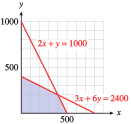
\includegraphics[width=0.5\linewidth]{images/fig-feasible-solutions}
\caption{\label{fig-feasible-solutions}}
\end{figure}
%
\begin{example}[]\label{example-TrailGear}
\leavevmode%
\begin{enumerate}[label=\alph*]
\item\hypertarget{li-1}{}Verify that the points \((300, 100)\) and \((200, 300)\) represent feasible solutions for the problem above. Show that \((300, 400)\) is not a feasible solution.%
\item\hypertarget{li-2}{}Find the values of the objective function \(P = 8x + 10y\) at the two feasible solutions in part (a).%
\end{enumerate}
%
\par\medskip\noindent%
\textbf{Solution.}\quad \leavevmode%
\begin{enumerate}[label=\alph*]
\item\hypertarget{li-3}{}The two points \((300, 100)\) and \((200, 300)\) lie within the shaded region in \hyperref[fig-feasible-solutions]{Figure~\ref{fig-feasible-solutions}}, but \((300, 400)\) does not. We can also verify that the coordinates of \((300, 100)\) and \((200, 300)\) satisfy each of the constraint inequalities.%
\item\hypertarget{li-4}{}For \((300, 100)\), we have%
\begin{equation*}
P = 8(\alert{300}) + 10(\blert{100}) = 3400
\end{equation*}
For \((200, 300)\), we have%
\begin{equation*}
P = 8(\alert{200}) + 10(\blert{300}) = 4600
\end{equation*}
%
\end{enumerate}
%
\end{example}
\begin{exercise}\label{exercise-1}
\leavevmode%
\begin{enumerate}[label=\alph*]
\item\hypertarget{li-5}{}Determine which of the points \((0, 400)\), \((400, 200)\), \((500, 0)\), and \((500, 400)\) represent feasible solutions for the TrailGear problem.%
\item\hypertarget{li-6}{}Find the values of the objective function \(P = 8x + 10y\) at the feasible solutions in part (a).%
\end{enumerate}
%
\end{exercise}
\typeout{************************************************}
\typeout{Subsection 1.1.3 The Optimum Solutions}
\typeout{************************************************}
\subsection[{The Optimum Solutions}]{The Optimum Solutions}\label{subsection-3}
We cannot check all of the feasible solutions to see which one results in the largest profit. Fortunately, there is a simple way to find the optimal solution.%
\par
Consider the objective function,%
\begin{equation*}
P = 8x + 10y
\end{equation*}
If TrailGear would like to make \(\$2000\) on hiking boots, it could produce \(200\) pairs of Sierra boots, or \(250\) pairs of Weekenders. Or it could produce some of each; for example, \(50\) pairs of Weekenders and \(160\) pairs of Sierra boots. In fact, every point on the line%
\begin{equation*}
8x + 10y = 2000
\end{equation*}
represents a combination of Weekenders and Sierra boots that will yield a profit of \(\$2000\). This line is labeled \(P = 2000\) in \hyperref[fig-objective-function-contours-over-feasibles]{Figure~\ref{fig-objective-function-contours-over-feasibles}}.%
\leavevmode%
\begin{figure}
\centering
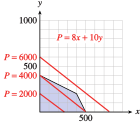
\includegraphics[width=0.5\linewidth]{images/fig-objective-function-contours-over-feasibles}
\caption{\label{fig-objective-function-contours-over-feasibles}}
\end{figure}
\par
If TrailGear would like to make \(\$4000\) on boots, it should choose a point on the line labeled \(P = 4000\). Similarly, all the points on the line labeled \(P = 6000\) will yield a profit of \(\$6000\), and so on. Different values of \(P\) correspond to parallel lines on the graph. Smaller values of \(P\) correspond to lines near the origin, and larger values of \(P\) have lines farther from the origin. Here is another example.%
\begin{example}[]\label{example-2}
\hyperref[fig-feasible-solutions2]{Figure~\ref{fig-feasible-solutions2}} shows the feasible solutions for another linear programming problem. The objective function is \(C = 3x + 5y\). \leavevmode%
\begin{figure}
\centering
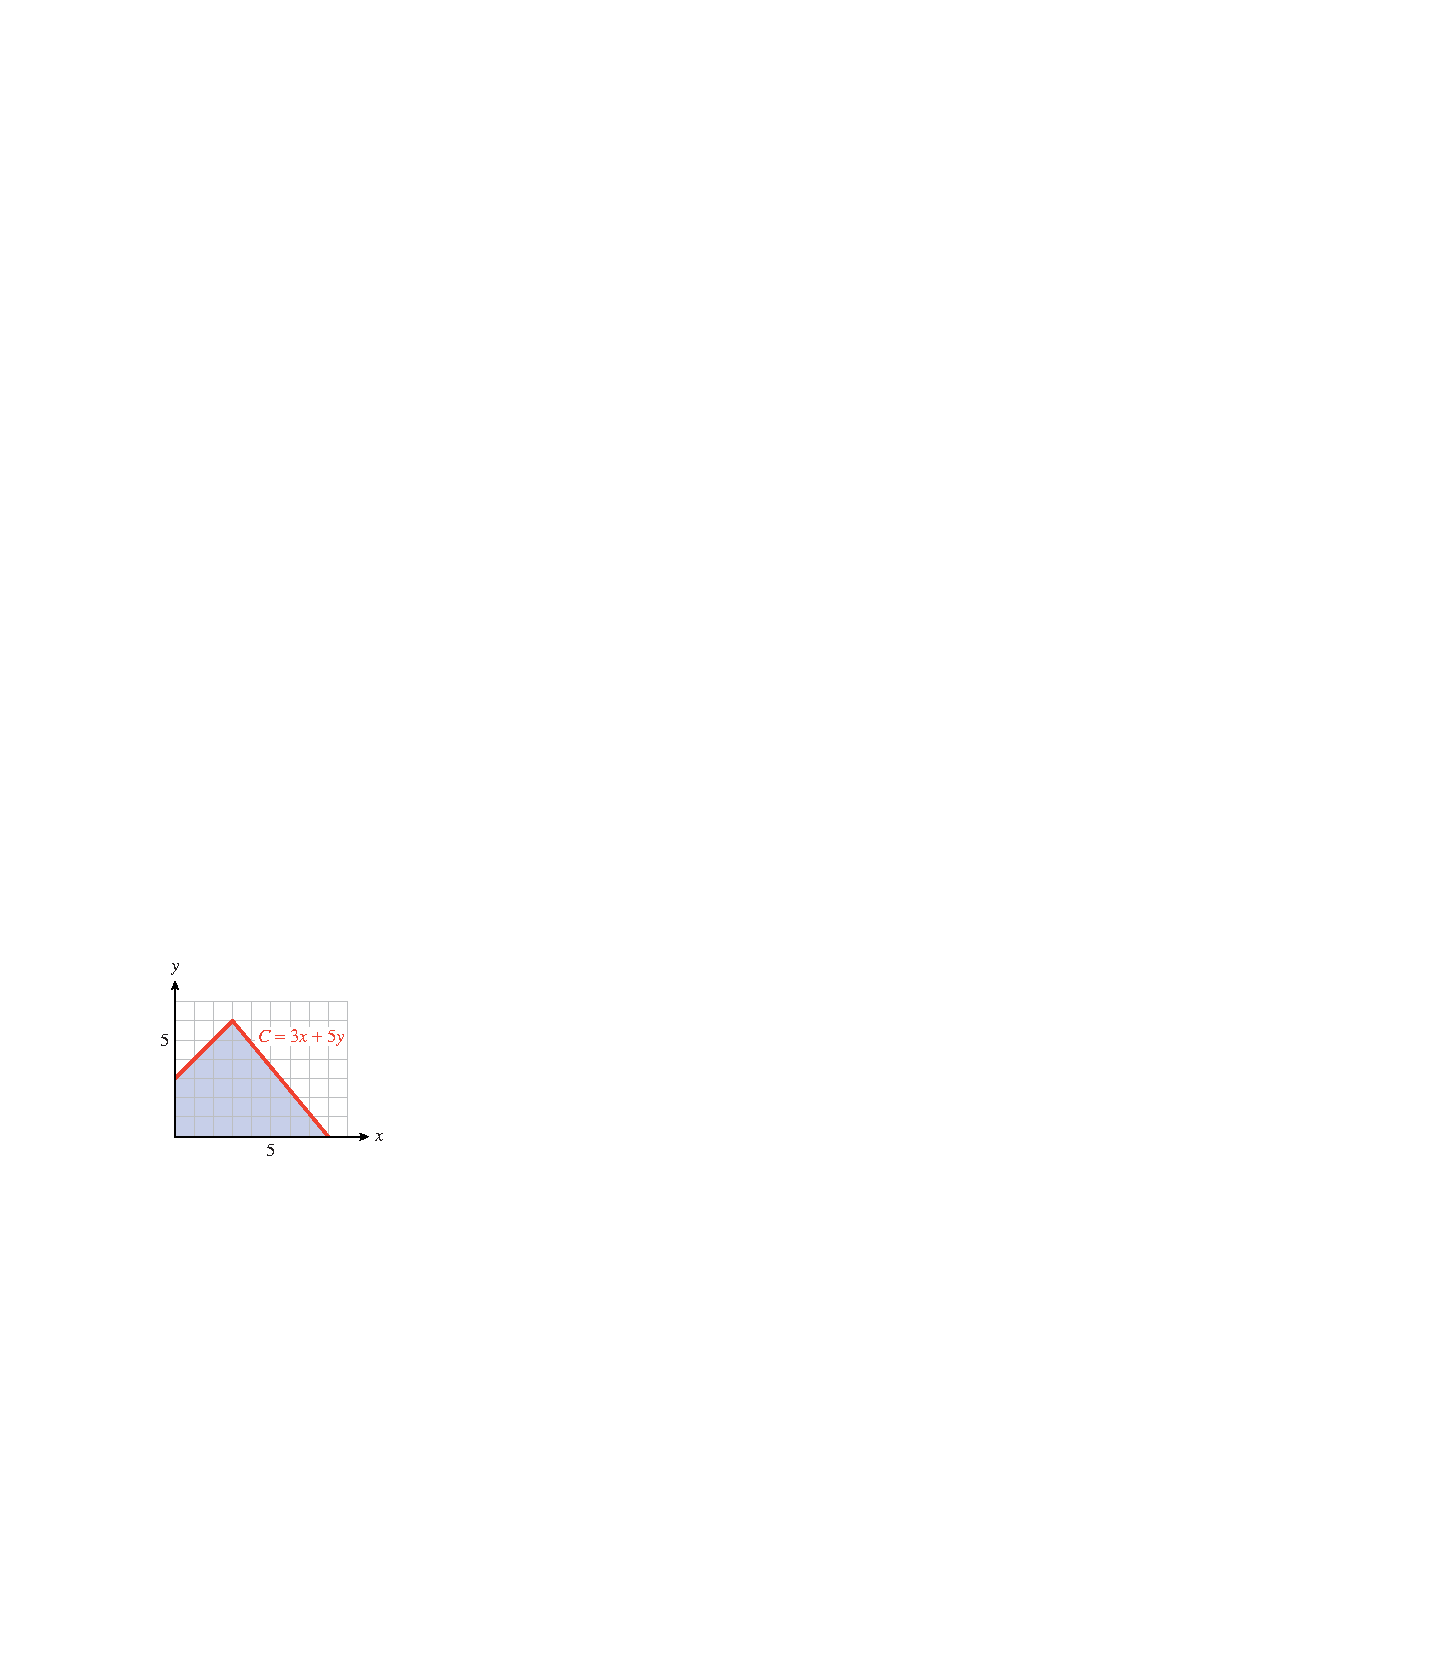
\includegraphics[width=0.5\linewidth]{images/fig-feasible-solutions2}
\caption{\label{fig-feasible-solutions2}}
\end{figure}
 \leavevmode%
\begin{enumerate}[label=\alph*]
\item\hypertarget{li-9}{}Find the value of \(C\) at the point \((0, 3)\). Are there other feasible solutions that give the same value of \(C\)?%
\item\hypertarget{li-10}{}Find all feasible solutions that result in an objective value of \(30\).%
\item\hypertarget{li-11}{}How many feasible solutions result in an objective value of \(39\)?%
\item\hypertarget{li-12}{}Is it possible for a feasible solution to result in an objective value of 45?%
\end{enumerate}
%
\par\medskip\noindent%
\textbf{Solution.}\quad \leavevmode%
\begin{enumerate}[label=\alph*]
\item\hypertarget{li-13}{}The objective value at the point \((0, 3)\) is%
\begin{equation*}
C = 3(\alert{0}) + 5(\blert{3}) = 15
\end{equation*}
Another point with the same objective value is \((5, 0)\). In fact, all points on the line \(3x + 5y = 15\) have an objective value of \(15\). This line intersects the set of feasible solutions in a line segment, as shown in Figure \hyperref[fig-feasible-solutions3]{Figure~\ref{fig-feasible-solutions3}}. Thus, there are infinitely many feasible solutions with objective value \(15\). \leavevmode%
\begin{figure}
\centering
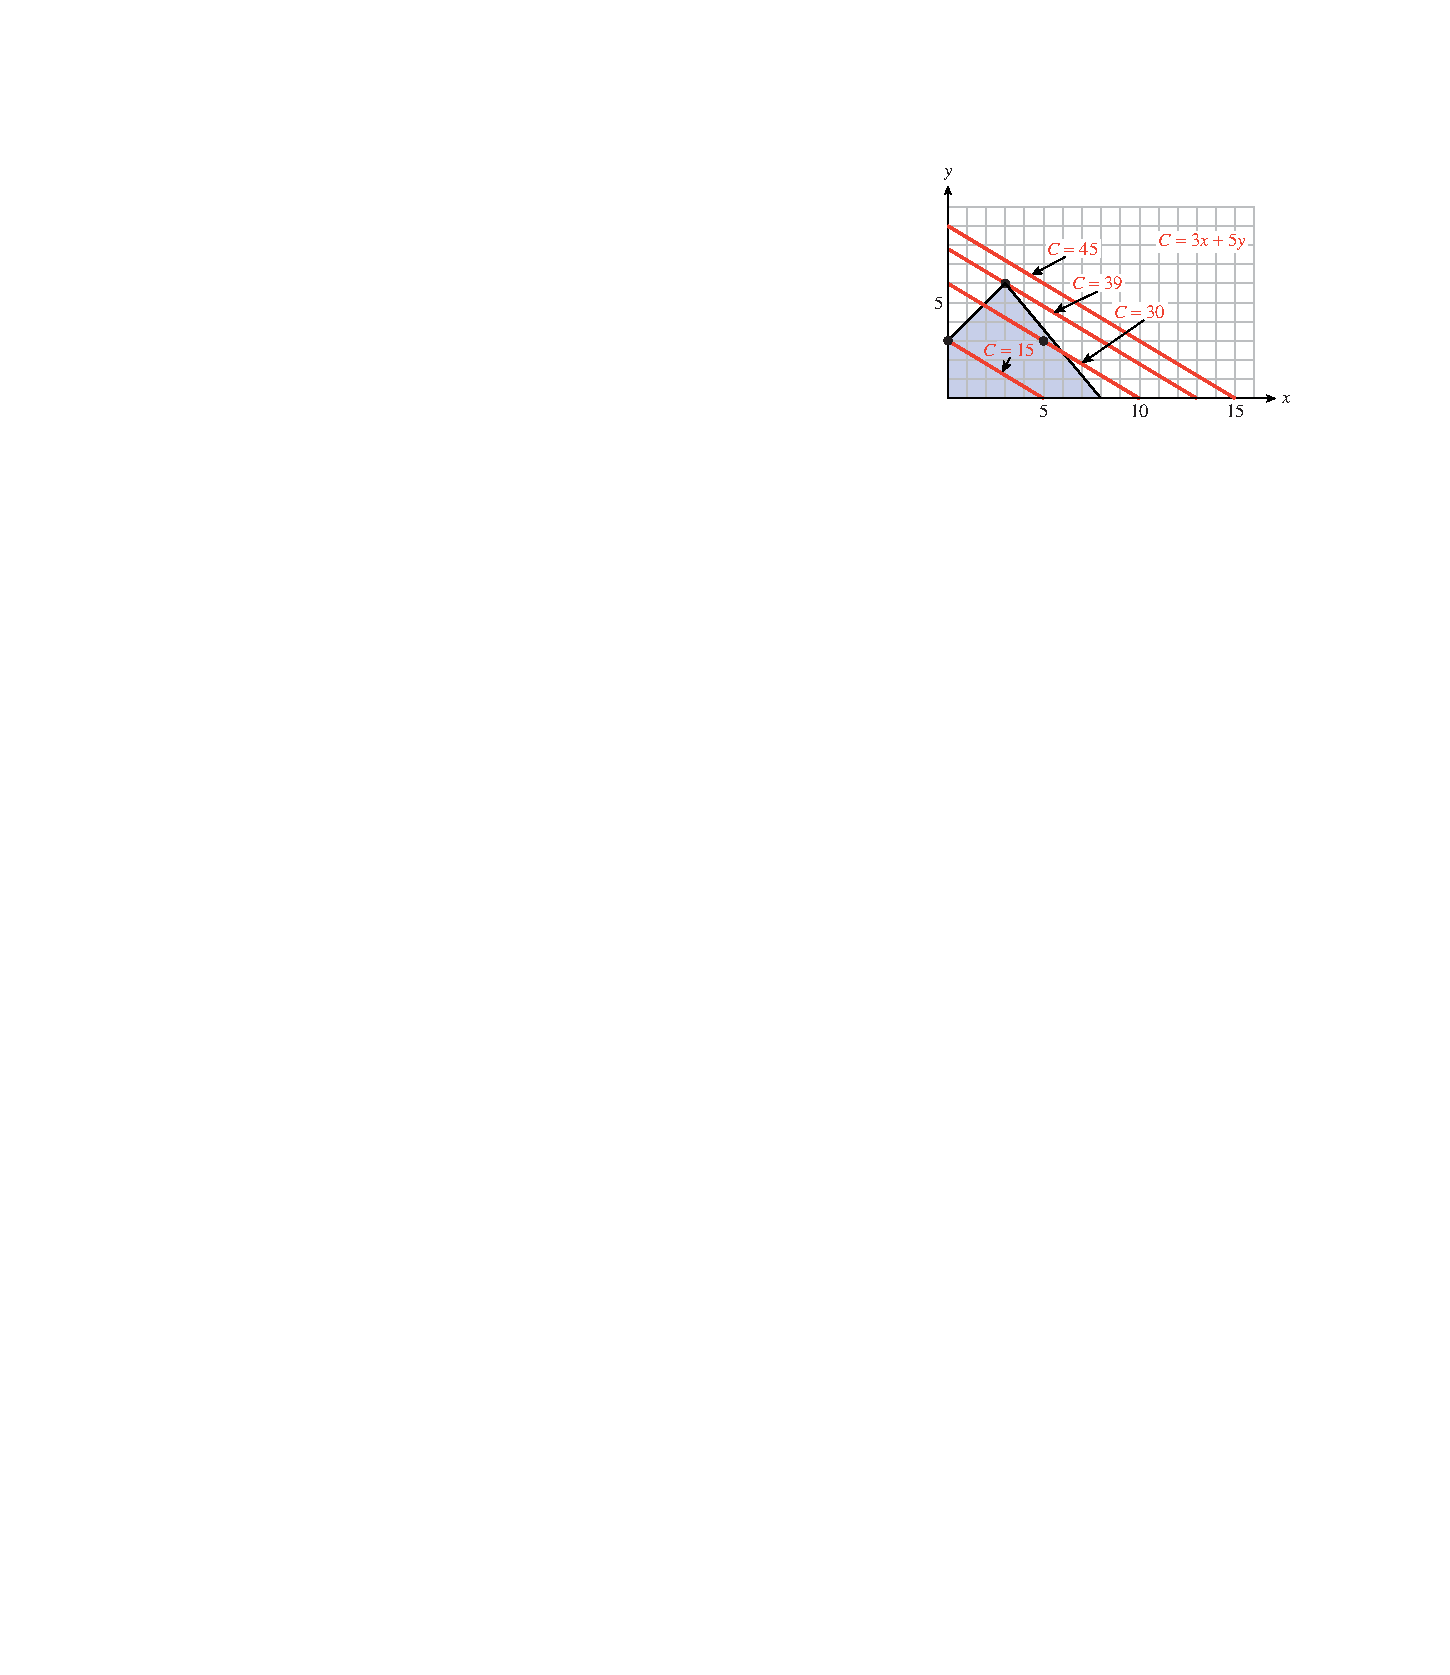
\includegraphics[width=0.7\linewidth]{images/fig-feasible-solutions3}
\caption{\label{fig-feasible-solutions3}}
\end{figure}
%
\item\hypertarget{li-14}{}Points that give an objective value of \(C = 30\) lie on the line \(3x + 5y = 30\), as shown in the figure. There are infinitely many feasible solutions that lie on this line; for example, one such point is \((5, 3)\).%
\item\hypertarget{li-15}{}The line \(3x + 5y = 39\) intersects the set of feasible solutions in only one point, the point \((3, 6)\). This is the only feasible solution that yields an objective value of \(39\).%
\item\hypertarget{li-16}{}The line \(3x + 5y = 45\) includes all points for which \(C=45\). This line does not intersect the set of feasible solutions, as we see in the figure. Thus, there are no feasible solutions that result in an objective value of \(45\).%
\end{enumerate}
%
\end{example}
\begin{exercise}\label{exercise-2}
\leavevmode%
\begin{enumerate}[label=\alph*]
\item\hypertarget{li-17}{}Returning to the TrailGear problem of \hyperref[example-TrailGear]{Example~\ref{example-TrailGear}}, find all feasible solutions for which the objective function \(P = 8x + 10y\) has a value of \(5200\).%
\item\hypertarget{li-18}{}Find all feasible solutions that result in an objective value of \(6000\).%
\end{enumerate}
%
\end{exercise}
\par
We are only allowed to choose points from the set of feasible solutions. Imagine the parallel lines representing different values of the objective function sweeping across the graph of the feasible solutions. The objective values increase as the lines sweep up across the graph. What is the last feasible solution the lines intersect before leaving the shaded region? If you study the preceding examples, perhaps you can see that the largest (and smallest) values of the objective function will occur at corner points of the set of feasible solutions. We have not proved this fact, but it is true.%
\begin{assemblage}{Linear Programming}\label{assemblage-1}
The maximum and the minimum values of the objective function always occur at vertices of the graph of feasible solutions.%
\end{assemblage}
\par
Depending on the exact formula for the objective function, the maximum and minimum values may occur at \emph{any} of the vertices of the shaded region.%
\begin{example}[]\label{example-3}
Find TrailGear's maximum weekly profit%
\par\medskip\noindent%
\textbf{Solution.}\quad \hyperref[fig-feasible-solutions4]{Figure~\ref{fig-feasible-solutions4}} shows the lines corresponding to the objective values \(P = 2000\), \(P = 4000\), and \(P = 5200\). The maximum value of the profit, \(P\), corresponds to the topmost line that intersects the region of feasible solutions. This is the line that passes through the vertex where the lines \(3x + 6y = 2400\) and \(2x + y = 1000\) intersect, namely the vertex at \((400, 200)\). The profit for that point is%
\begin{equation*}
P = 8(400) + 10(200) = 5200
\end{equation*}
so the maximum weekly profit is \(\$5200\).%
\leavevmode%
\begin{figure}
\centering
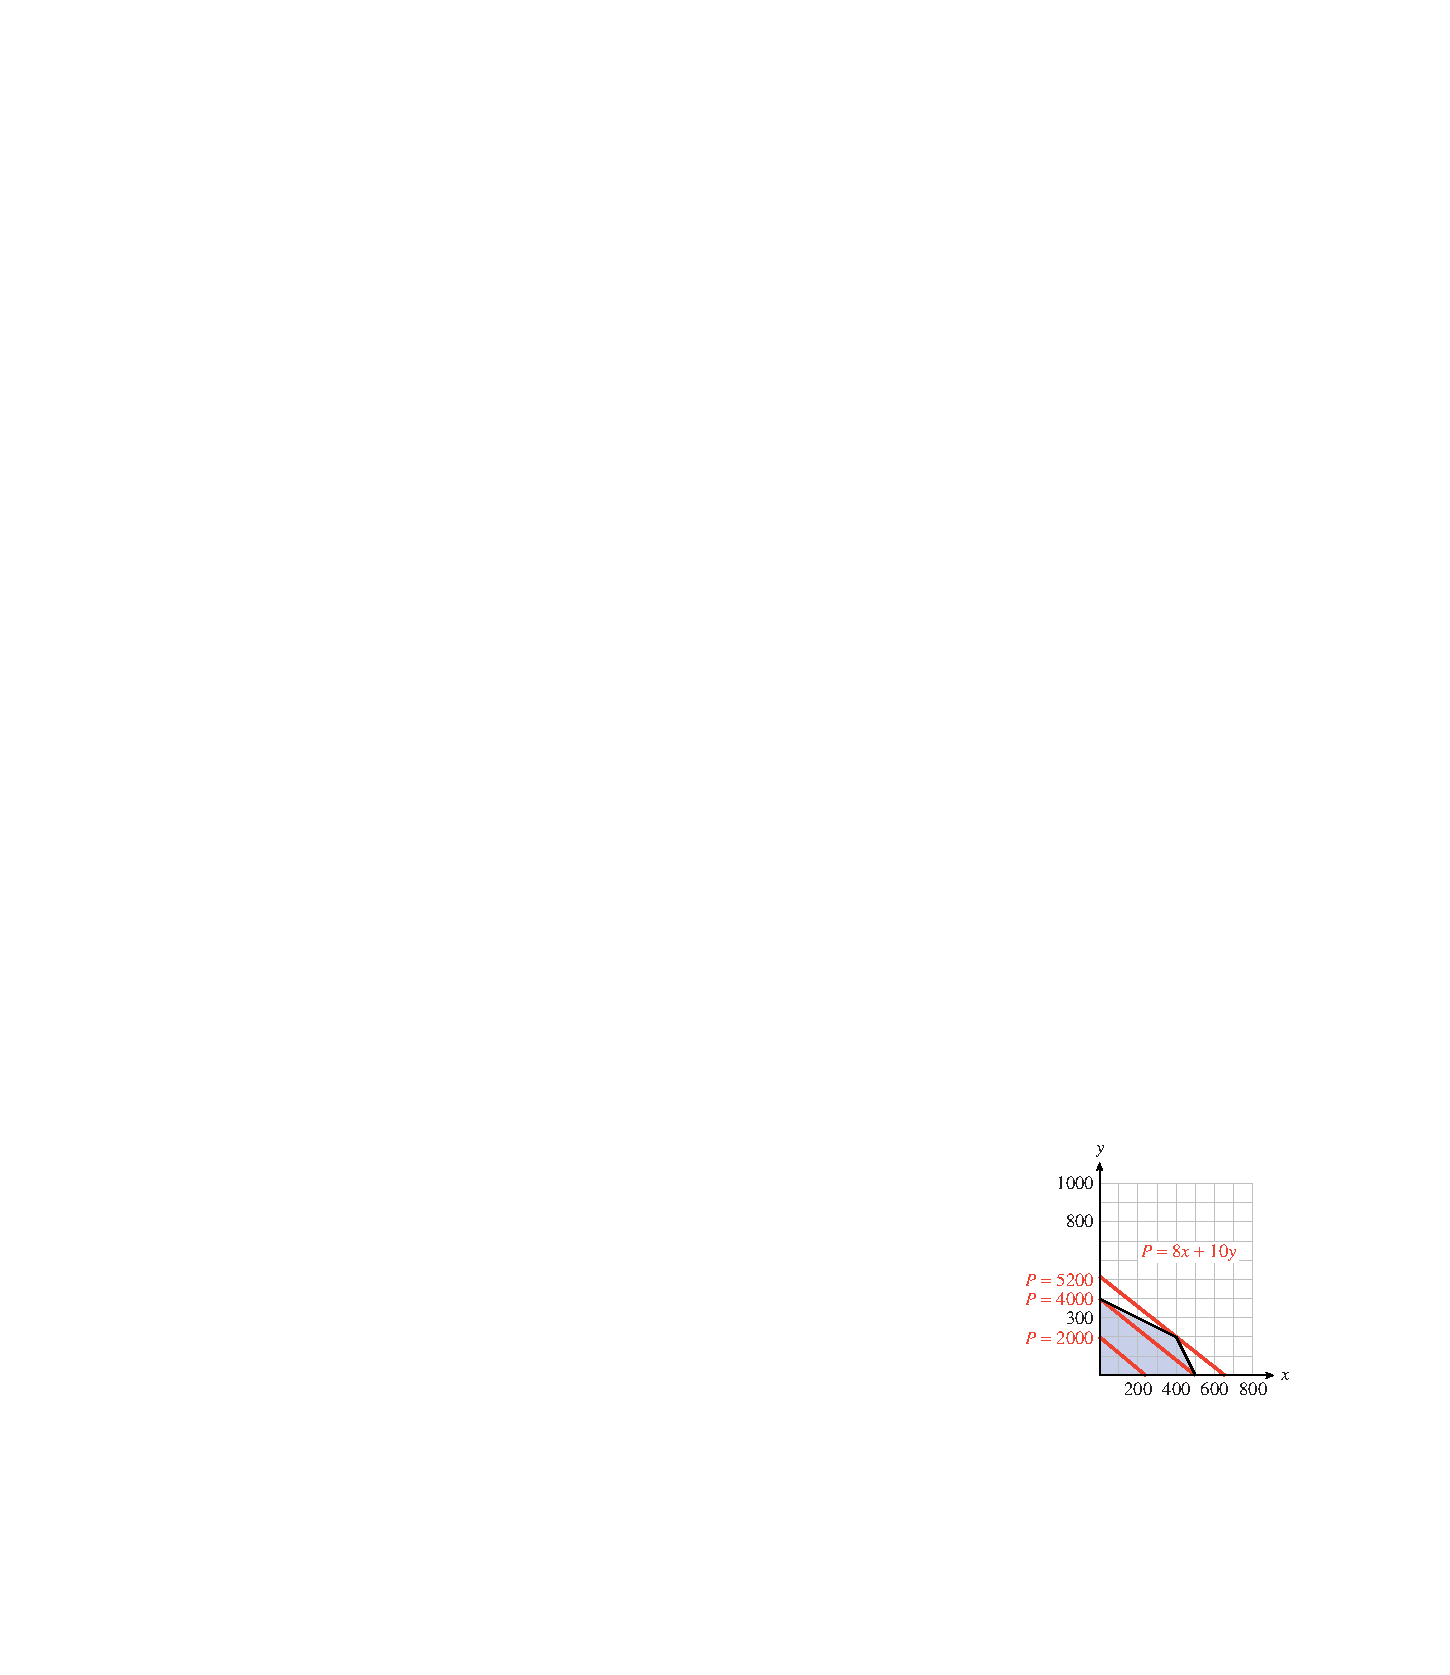
\includegraphics[width=0.5\linewidth]{images/fig-feasible-solutions4}
\caption{\label{fig-feasible-solutions4}}
\end{figure}
\end{example}
\begin{exercise}\label{exercise-3}
\hyperref[fig-feasible-solutions5]{Figure~\ref{fig-feasible-solutions5}} shows the feasible solutions for a linear programming problem. The objective function is \(R = x + 5y\). \leavevmode%
\begin{enumerate}[label=\alph*]
\item\hypertarget{li-21}{}Sketch lines for objective values of \(R=5\), \(R=15\), \(R = 25\), and \(R=35\).%
\item\hypertarget{li-22}{}Evaluate the objective function at each vertex of the shaded region.%
\item\hypertarget{li-23}{}Which vertex corresponds to the maximum value of the objective function? What is the maximum value?%
\item\hypertarget{li-24}{}Which vertex corresponds to the minimum value of the objective function? What is the minimum value?%
\end{enumerate}
 \leavevmode%
\begin{figure}
\centering
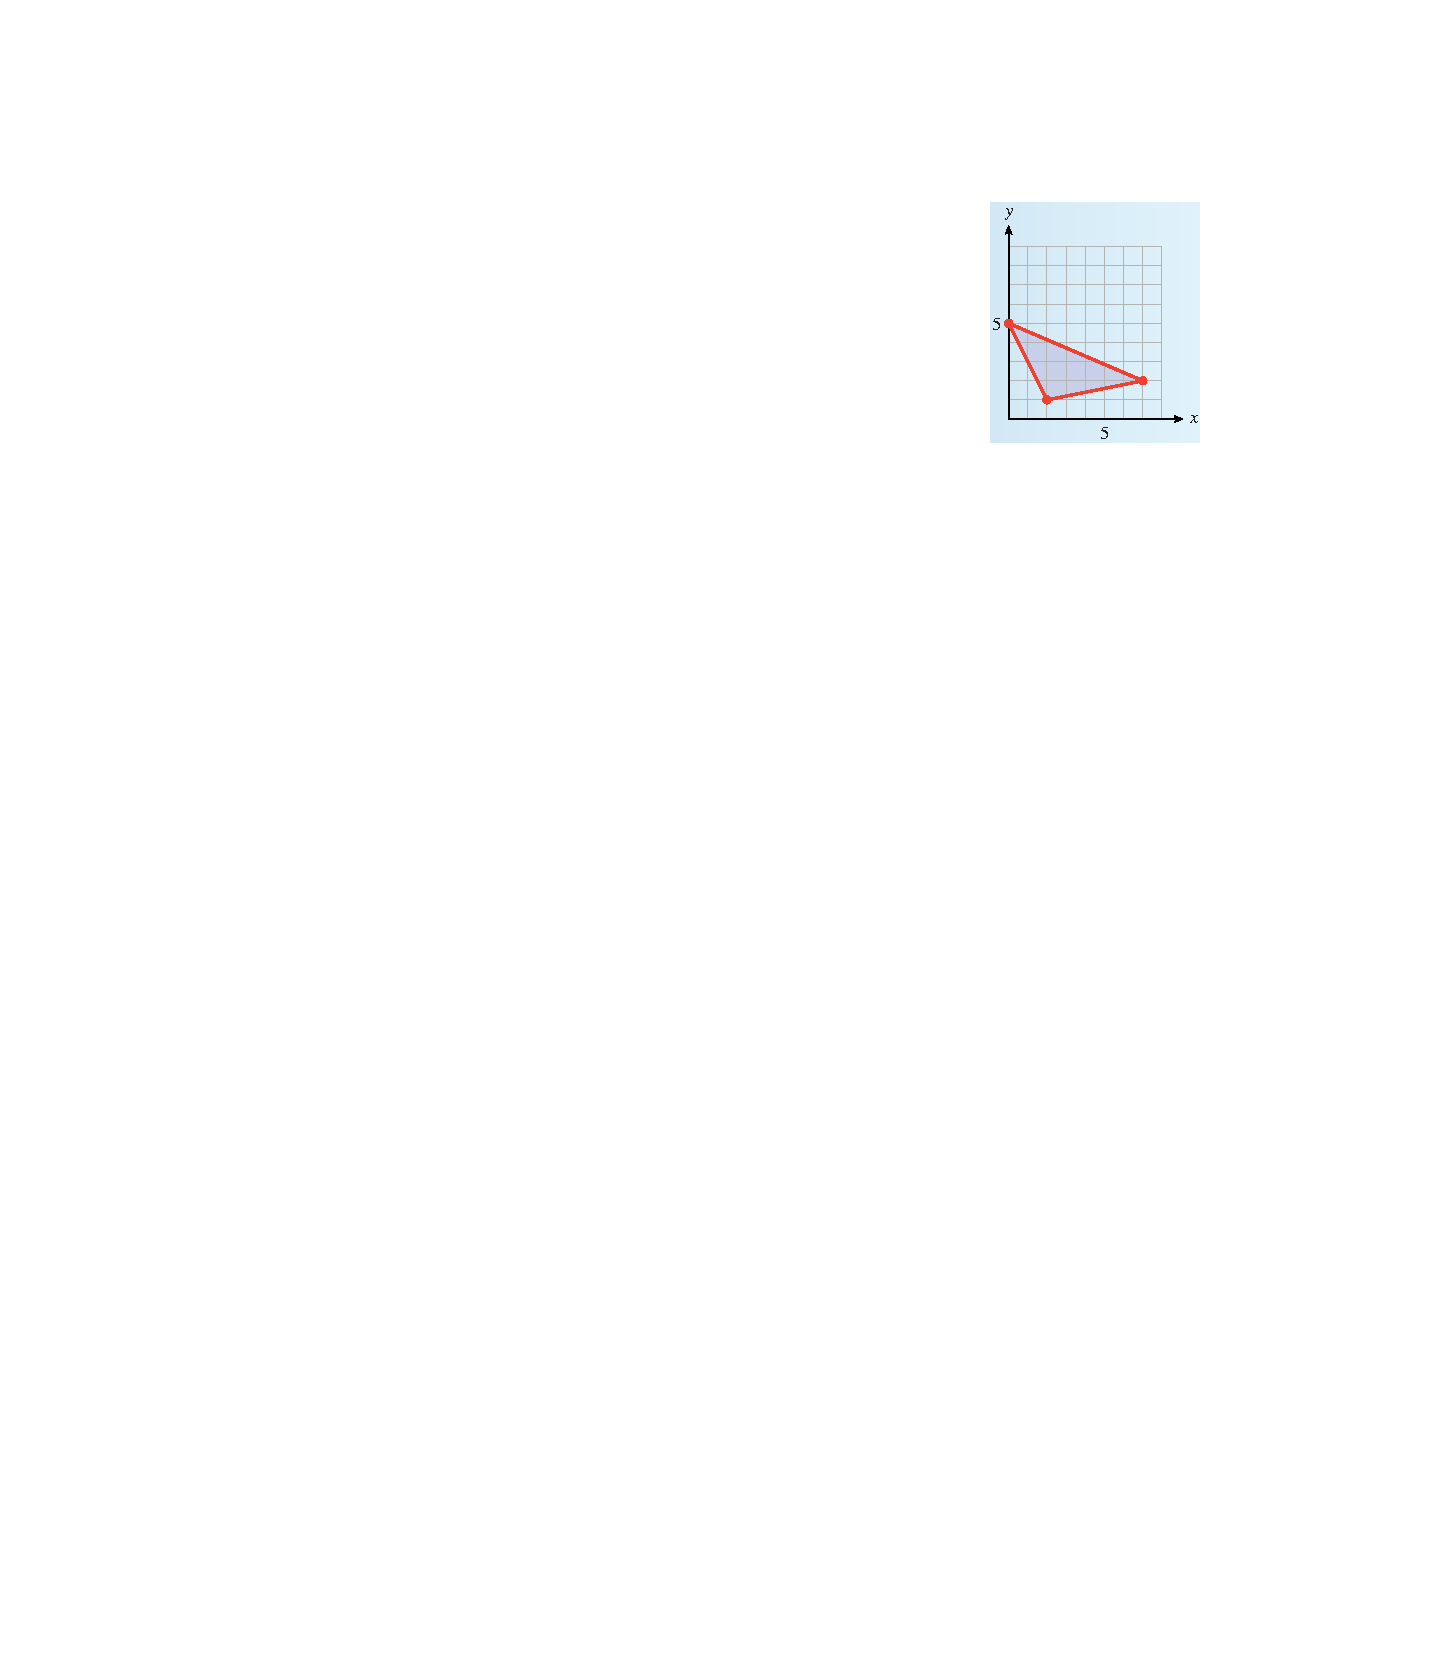
\includegraphics[width=0.5\linewidth]{images/fig-feasible-solutions5}
\caption{\label{fig-feasible-solutions5}}
\end{figure}
%
\end{exercise}
\par
We can now formulate a strategy for solving problems by linear programming.%
\begin{assemblage}{To Solve a Linear Programming Problem:}\label{assemblage-solve-linear-programming-problem}
\leavevmode%
\begin{enumerate}[label=*\arabic**]
\item\hypertarget{li-29}{}Represent the unknown quantities by variables. Write the objective function and the constraints in terms of the variables.%
\item\hypertarget{li-30}{}Graph the solutions to the constraint inequalities.%
\item\hypertarget{li-31}{}Find the coordinates of each vertex of the solution set.%
\item\hypertarget{li-32}{}Evaluate the objective function at each vertex.%
\item\hypertarget{li-33}{}The maximum and minimum values of the objective function occur at vertices of the set of feasible solutions.%
\end{enumerate}
%
\end{assemblage}
\par
In \hyperref[example-unbounded-feasible-set]{Example~\ref{example-unbounded-feasible-set}}, the set of feasible solutions is an unbounded region.%
\begin{example}[]\label{example-unbounded-feasible-set}
Each week, the Healthy Food Store buys both granola and muesli in bulk from two cereal companies. The store requires at least \(12\) kilograms of granola and \(9\) kilograms of muesli. Company A charges \(\$15\) for a package that contains \(2\) kilograms of granola and \(1\) kilogram of muesli. Company B charges \(\$25\) for a package of \(3\) kilograms of granola and \(3\) kilograms of muesli. How much should the Healthy Food Store purchase from each company in order to minimize its costs and still meet its needs for granola and muesli? What is the minimum cost?%
\par\medskip\noindent%
\textbf{Solution.}\quad \leavevmode%
\begin{description}
\item[{Step 1:}]\hypertarget{li-34}{}%
\begin{gather*}
\text{Number of packages purchased from Company A: } ~x\\
\text{Number of packages purchased from Company B: } ~y
\end{gather*}
First write the objective function. The store would like to minimize its cost, so%
\begin{equation*}
C = 15x + 25y
\end{equation*}
Next, write the constraints. These will be a system of inequalities. It may help to organize the information into a table. \leavevmode%
\begin{table}
\centering
\begin{tabular}{AcAcAcAcA}\hrulethin
&Company A&Company B&Required\tabularnewline\hrulethin
Granola&\(2x\)&\(3y\)&12\tabularnewline\hrulethin
Muesli&\(x\)&\(3y\)&9\tabularnewline\hrulethin
\end{tabular}
\end{table}
 The Healthy Food Store will have \(2x\) kilograms of granola and \(x\) kilograms of muesli from Company A, and \(3y\) kilograms of granola and \(3y\) kilograms of muesli from Company B. The store requires that%
\begin{align*}
2x + 3y \amp\ge 12\\
x + 3y \amp\ge 9
\end{align*}
Because the store cannot purchase negative quantities, we also have%
\begin{equation*}
x \ge 0, ~~~~~y \ge 0
\end{equation*}
%
\item[{Step 2:}]\hypertarget{li-35}{}Graph the solutions to the constraint system. The feasible solutions form the shaded region shown in \hyperref[fig-unbounded-feasible-set]{Figure~\ref{fig-unbounded-feasible-set}}. Any ordered point on this graph corresponds to a way to purchase granola and muesli that meets the store’s needs, but some of these choices cost more than others. \leavevmode%
\begin{figure}
\centering
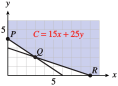
\includegraphics[width=0.6\linewidth]{images/fig-unbounded-feasible-set}
\caption{\label{fig-unbounded-feasible-set}}
\end{figure}
%
\item[{Step 3:}]\hypertarget{li-36}{}We know that the minimum cost will occur at one of the vertex points, which are labeled in the figure. The coordinates of \(P\) and \(R\) are easy to see. To find the coordinates of \(Q\), we notice that it is the intersection of the lines \(2x + 3y = 12\) and \(x + 3y = 9\). Thus, we must solve the system%
\begin{align*}
2x + 3y \amp= 12\\
x + 3y \amp = 9
\end{align*}
Subtracting the second equation from the first, we find that \(x=3\). Substituting this value into either of the original two equations, we find that \(y=2\). Thus the point \(Q\) has coordinates \((3, 2)\).%
\item[{Step 4:}]\hypertarget{li-37}{}Now we evaluate the objective function at each of the three vertices.%
\begin{align*}
\amp\text{At }P (0, 4): \amp C \amp= 15(\alert{0})+ 25(\blert{4}) = 100{}
\\
\amp\text{At }P (3,2):\amp C \amp= 15(\alert{3})+ 25(\blert{2}) = 95{}\amp\amp\text{Minimum cost}
\\
\amp\text{At }P (9,0): \amp C \amp= 15(\alert{9})+ 25(\blert{0}) = 135{}\amp
\end{align*}
The minimum cost occurs at point \(Q\).%
\item[{Step 5:}]\hypertarget{li-38}{}The Healthy Food Store should buy three packages from Company A and two packages from Company B. It will pay \(\$95\) for its stock of granola and muesli.%
\end{description}
%
\end{example}
\begin{exercise}\label{exercise-4}
Find the minimum value of the objective function, \(O = 5x + 3y\), subject to the constraints \(x\ge 0\), \(y\ge 0\), \(x + y \ge 7\), and \(5x + 2y \ge 20\).%
\end{exercise}
\begin{remark}[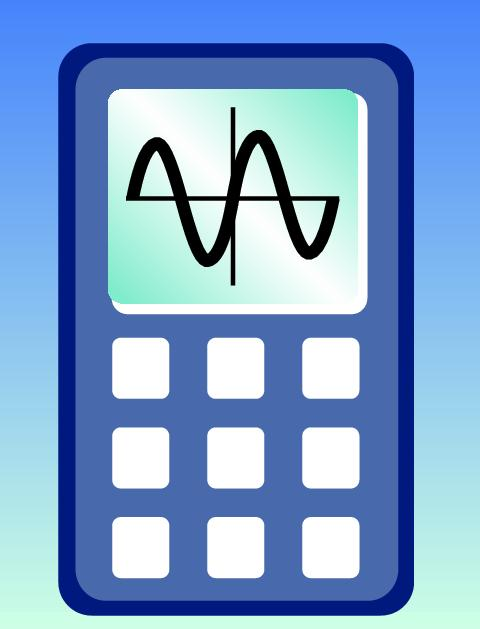
\includegraphics[width=0.08\linewidth]{images/icon-GC.jpg}
Using a Graphing Calculator]\label{remark-1}
You can use your graphing calculator to solve the problem in \hyperref[example-unbounded-feasible-set]{Example~\ref{example-unbounded-feasible-set}}. Set the window values at%
\begin{align*}
\text{Xmin} \amp = 0 \amp\amp \text{Xmax} = 9.4
\\
\text{Ymin} \amp = 0 \amp\amp \text{Ymax} = 6.2
\end{align*}
Next, graph the set of feasible solutions. We have already taken care of the constraints \(x\ge 0\) and \(y\ge 0\) by setting \(Xmin\) and \(Ymin\) to zero. Solve each of the other constraints for \(y\) to get%
\begin{align*}
y \amp\ge (12 − 2x)/3\\
y \amp\ge(9 − x)/3
\end{align*}
For each constraint, the set of feasible solutions lies above the boundary line, because \(y\) is greater than the expression in \(x\). To shade the regions above the graphs of \(Y_1\) and \(Y_2\), move the cursor onto the backslash in front of the equations and press \lstinline?ENTER? twice, as shown in \hyperref[fig-GC-feasible]{Figure~\ref{fig-GC-feasible}}a. Then press \lstinline?GRAPH?. Your display should look like \hyperref[fig-GC-feasible]{Figure~\ref{fig-GC-feasible}}b. \leavevmode%
\begin{figure}
\centering
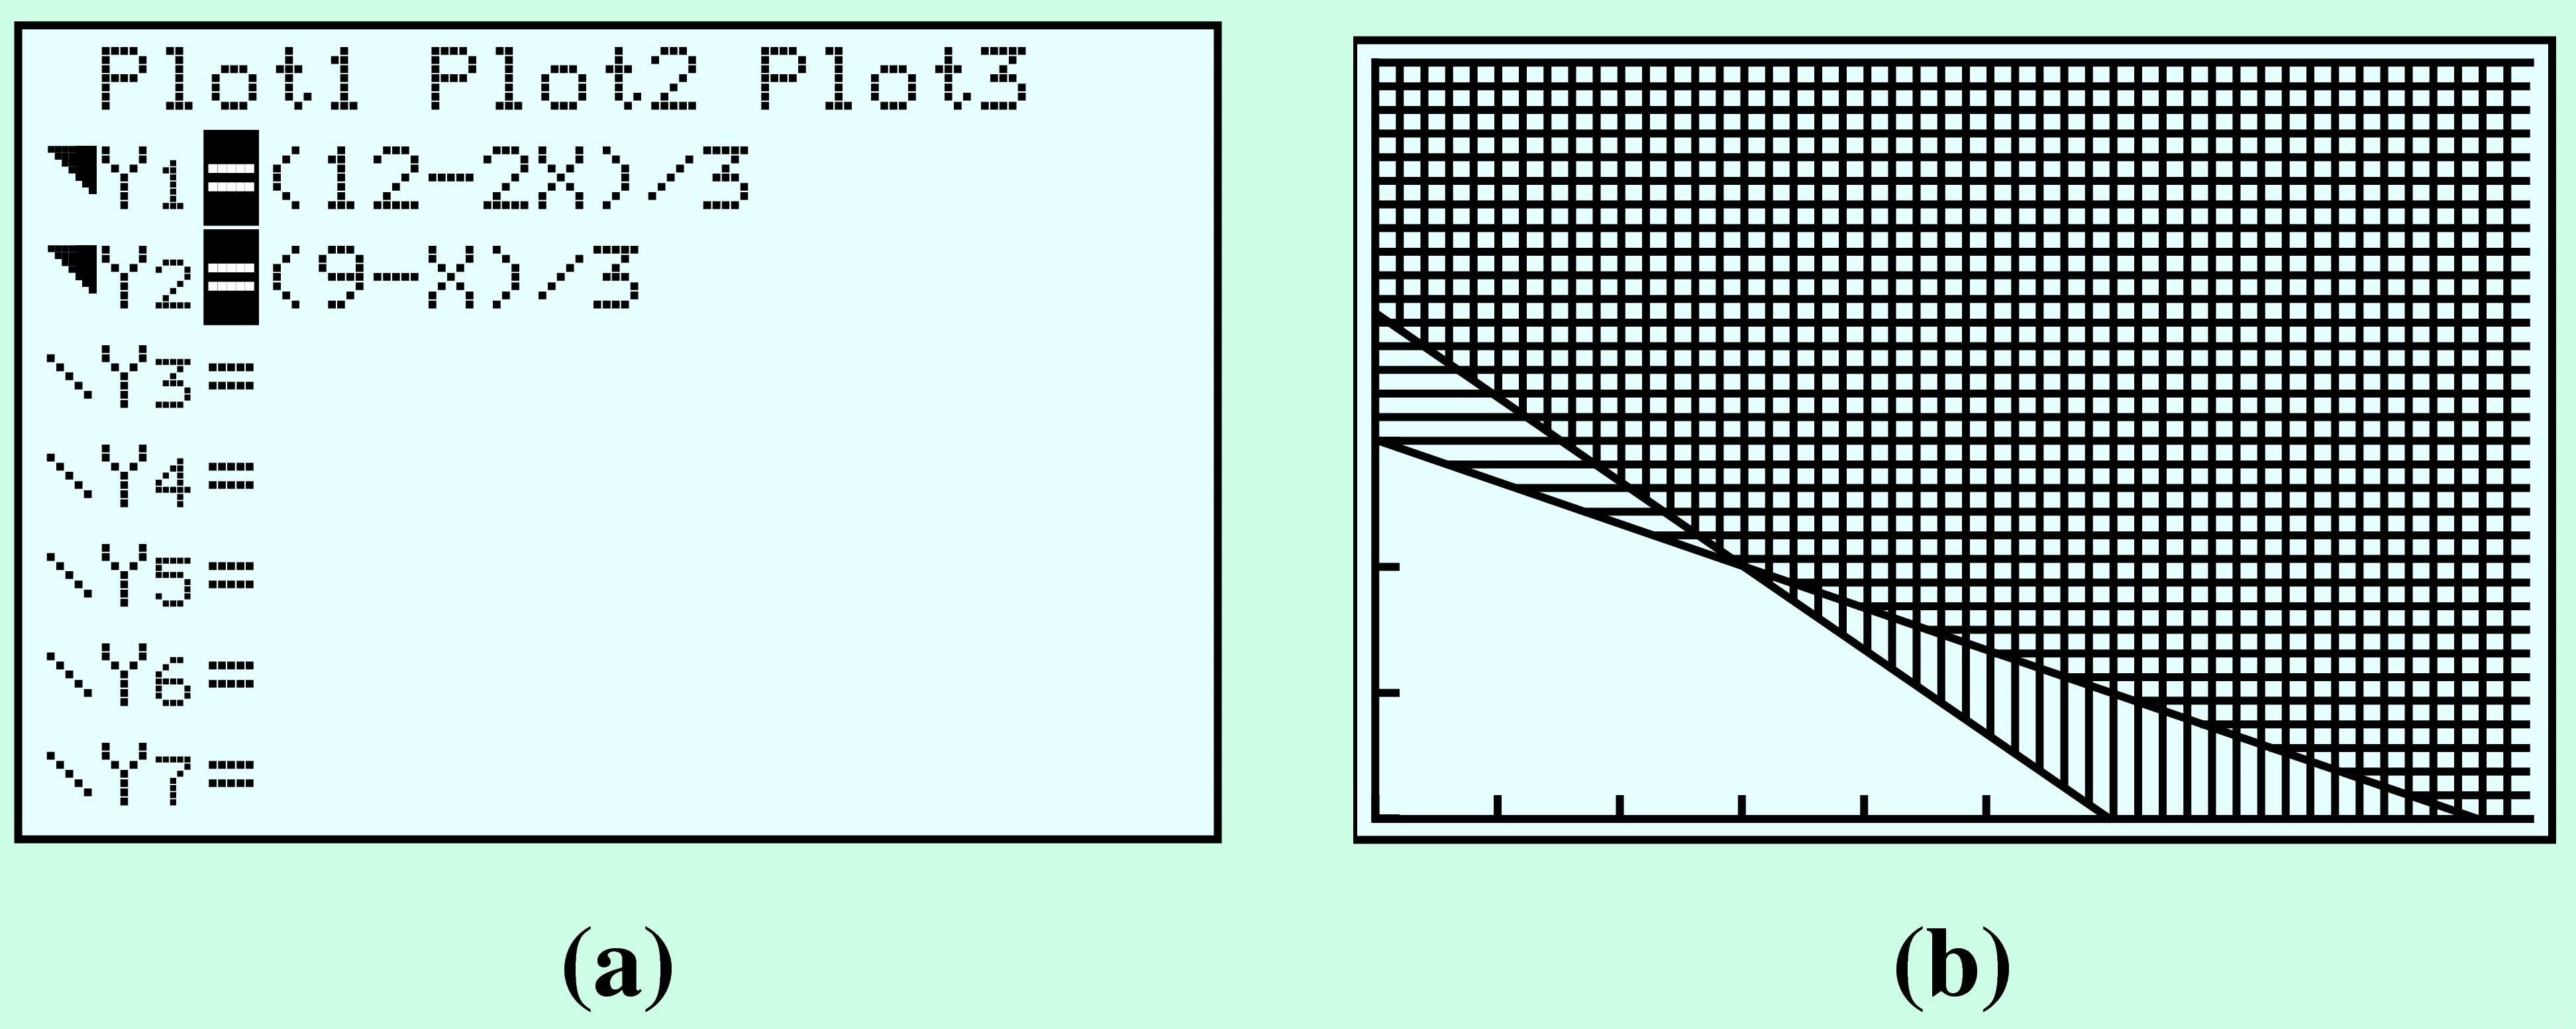
\includegraphics[width=0.8\linewidth]{images/fig-GC-feasible.jpg}
\caption{\label{fig-GC-feasible}}
\end{figure}
%
\par
The feasible solutions lie in the crosshatched region that is shaded with both the vertical and horizontal lines. We will use the calculator to evaluate the objective function at each vertex. First, use the \lstinline?TRACE? (or \emph{value} or \(intersect\) feature) to find the coordinates of one of the vertices, say \((0, 4)\). Then press \lstinline?2nd? \lstinline?QUIT? to get back to the \emph{Home} screen; enter the formula for the objective function by keying in%
\begin{equation*}
15X + 25Y
\end{equation*}
(Enter \(Y\) by pressing \lstinline?ALPHA? \(1\).) Your calculator has stored the values \(x=0\) and \(y=4\) from the \lstinline?TRACE? key, so when you press \lstinline?ENTER?, the calculator returns \(100\) for the value of \(C\) at that point. Thus, when \(x=0\) and \(y=4\), \(C=100\).%
\par
Similarly, you can verify that \(C=135\) when \(x=9\) and \(y=0\), and that when \(x=3\) and \(y=2\), \(C-95\). Thus, the minimum cost of \(\$95\) occurs when \(x=3\) and \(y=2\).%
\end{remark}
\typeout{************************************************}
\typeout{Subsection 1.1.4 Section Summary}
\typeout{************************************************}
\subsection[{Section Summary}]{Section Summary}\label{summary-8-5}
\typeout{************************************************}
\typeout{Subsubsection 1.1.4.1 Vocabulary}
\typeout{************************************************}
\subsubsection[{Vocabulary}]{Vocabulary}\label{subsubsection-1}
Look up the definitions of new terms in the Glossary. \leavevmode%
\begin{multicols}{3}
\begin{itemize}[label=\textbullet]
\item{}Objective function%
\item{}Constraint%
\item{}Feasible solution%
\end{itemize}
\end{multicols}
%
\typeout{************************************************}
\typeout{Subsubsection 1.1.4.2 CONCEPTS}
\typeout{************************************************}
\subsubsection[{CONCEPTS}]{CONCEPTS}\label{subsubsection-2}
\leavevmode%
\begin{enumerate}[label=\arabic*]
\item\hypertarget{li-42}{}\terminology{Linear programming} is a technique for finding the maximum or minimum value of an \terminology{objective function}, subject to a system of \terminology{constraints}.%
\item\hypertarget{li-43}{}The optimum solution occurs at one of the vertices of the set of \terminology{feasible solutions}.%
\item\hypertarget{li-44}{}\hyperref[assemblage-solve-linear-programming-problem]{To Solve a Linear Programming Problem~}%
\end{enumerate}
%
\typeout{************************************************}
\typeout{Subsubsection 1.1.4.3 STUDY QUESTIONS}
\typeout{************************************************}
\subsubsection[{STUDY QUESTIONS}]{STUDY QUESTIONS}\label{subsubsection-3}
\leavevmode%
\begin{enumerate}[label=\arabic*]
\item\hypertarget{li-45}{}Explain the terms \terminology{objective function}, \terminology{constraints}, and \terminology{feasible solution}.%
\item\hypertarget{li-46}{}Explain how to solve a linear programming problem by graphing.%
\item\hypertarget{li-47}{}How can you find the vertices of the set of feasible solutions?%
\item\hypertarget{li-48}{}Where do the maximum and minimum values of the objective function occur?%
\end{enumerate}
%
\typeout{************************************************}
\typeout{Subsubsection 1.1.4.4 SKILLS}
\typeout{************************************************}
\subsubsection[{SKILLS}]{SKILLS}\label{subsubsection-4}
Practice each skill in the \hyperref[section-8-5-exercises]{Homework~\ref{section-8-5-exercises}} problems listed. \leavevmode%
\begin{enumerate}[label=\arabic*]
\item\hypertarget{li-49}{}Find the maximum or minimum value for an objective function and a given set of feasible solutions: #1\textendash{}12%
\item\hypertarget{li-50}{}Solve a linear programming problem by graphing: #13\textendash{}32%
\item\hypertarget{li-51}{}Write the objective function and the constraints for a linear programming problem: #19\textendash{}24%
\end{enumerate}
%
\typeout{************************************************}
\typeout{Exercises 1.1.5 Homework}
\typeout{************************************************}
\subsection[{Homework}]{Homework}\label{section-8-5-exercises}
\hypertarget{exercisegroup-1}{}\par\noindent For Problems 1\textendash{}4, find the minimum value of the cost function \(C = 3x+ 4y\) subject to following constraints:%
\begin{equation*}
x + y \ge 10, ~~x \le 8, ~~y \le 7, ~~x \ge 0, ~~y \ge 0
\end{equation*}
The graph of the feasible solutions is shown in in the figure. \leavevmode%
\begin{figure}
\centering
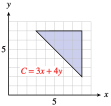
\includegraphics[width=0.35\linewidth]{images/fig-8-5-1}
\end{figure}
%
\begin{exercisegroup}(1)
\exercise[1.]\hypertarget{exercise-5}{}Use a graph to explain why it is impossible in this situation to have a cost as low as \(\$12\).%
\par\smallskip
\noindent\textbf{Hint.}\hypertarget{hint-1}{}\quad
Draw the graph of \(12 = 3x + 4y\) on the graph of the feasible solutions.)%
\par\smallskip
\noindent\textbf{Answer.}\hypertarget{answer-5}{}\quad
The graph of \(12 = 3x + 4y\) does not intersect the set of feasible solutions.%
\exercise[2.]\hypertarget{exercise-6}{}Use a graph to explain why the cost will not be as great as \(\$60\).%
\par\smallskip
\noindent\textbf{Hint.}\hypertarget{hint-2}{}\quad
Draw the graph of \(60 = 3x + 4y\) together with the graph of the feasible solutions.%
\exercise[3.]\hypertarget{exercise-7}{}Use a graph to determine which vertex of the shaded region will correspond to the minimum cost. What is the minimum cost?%
\par\smallskip
\noindent\textbf{Answer.}\hypertarget{answer-6}{}\quad
\((8, 2)\); \(\$32\)%
\exercise[4.]\hypertarget{exercise-8}{}Use a graph to determine which vertex of the shaded region will correspond to the maximum cost. What is the maximum cost?%
\end{exercisegroup}
\par\smallskip\noindent
\hypertarget{exercisegroup-2}{}\par\noindent For Problems 5\textendash{}8, find the minimum value of the profit function \(P = 4x - 2y\) subject to the following constraints:%
\begin{equation*}
5x- y \ge 22, ~~x + y\le 8, ~~x \ge 0, ~~y \ge 0
\end{equation*}
The graph of the feasible solutions is shown in the figure. \leavevmode%
\begin{figure}
\centering
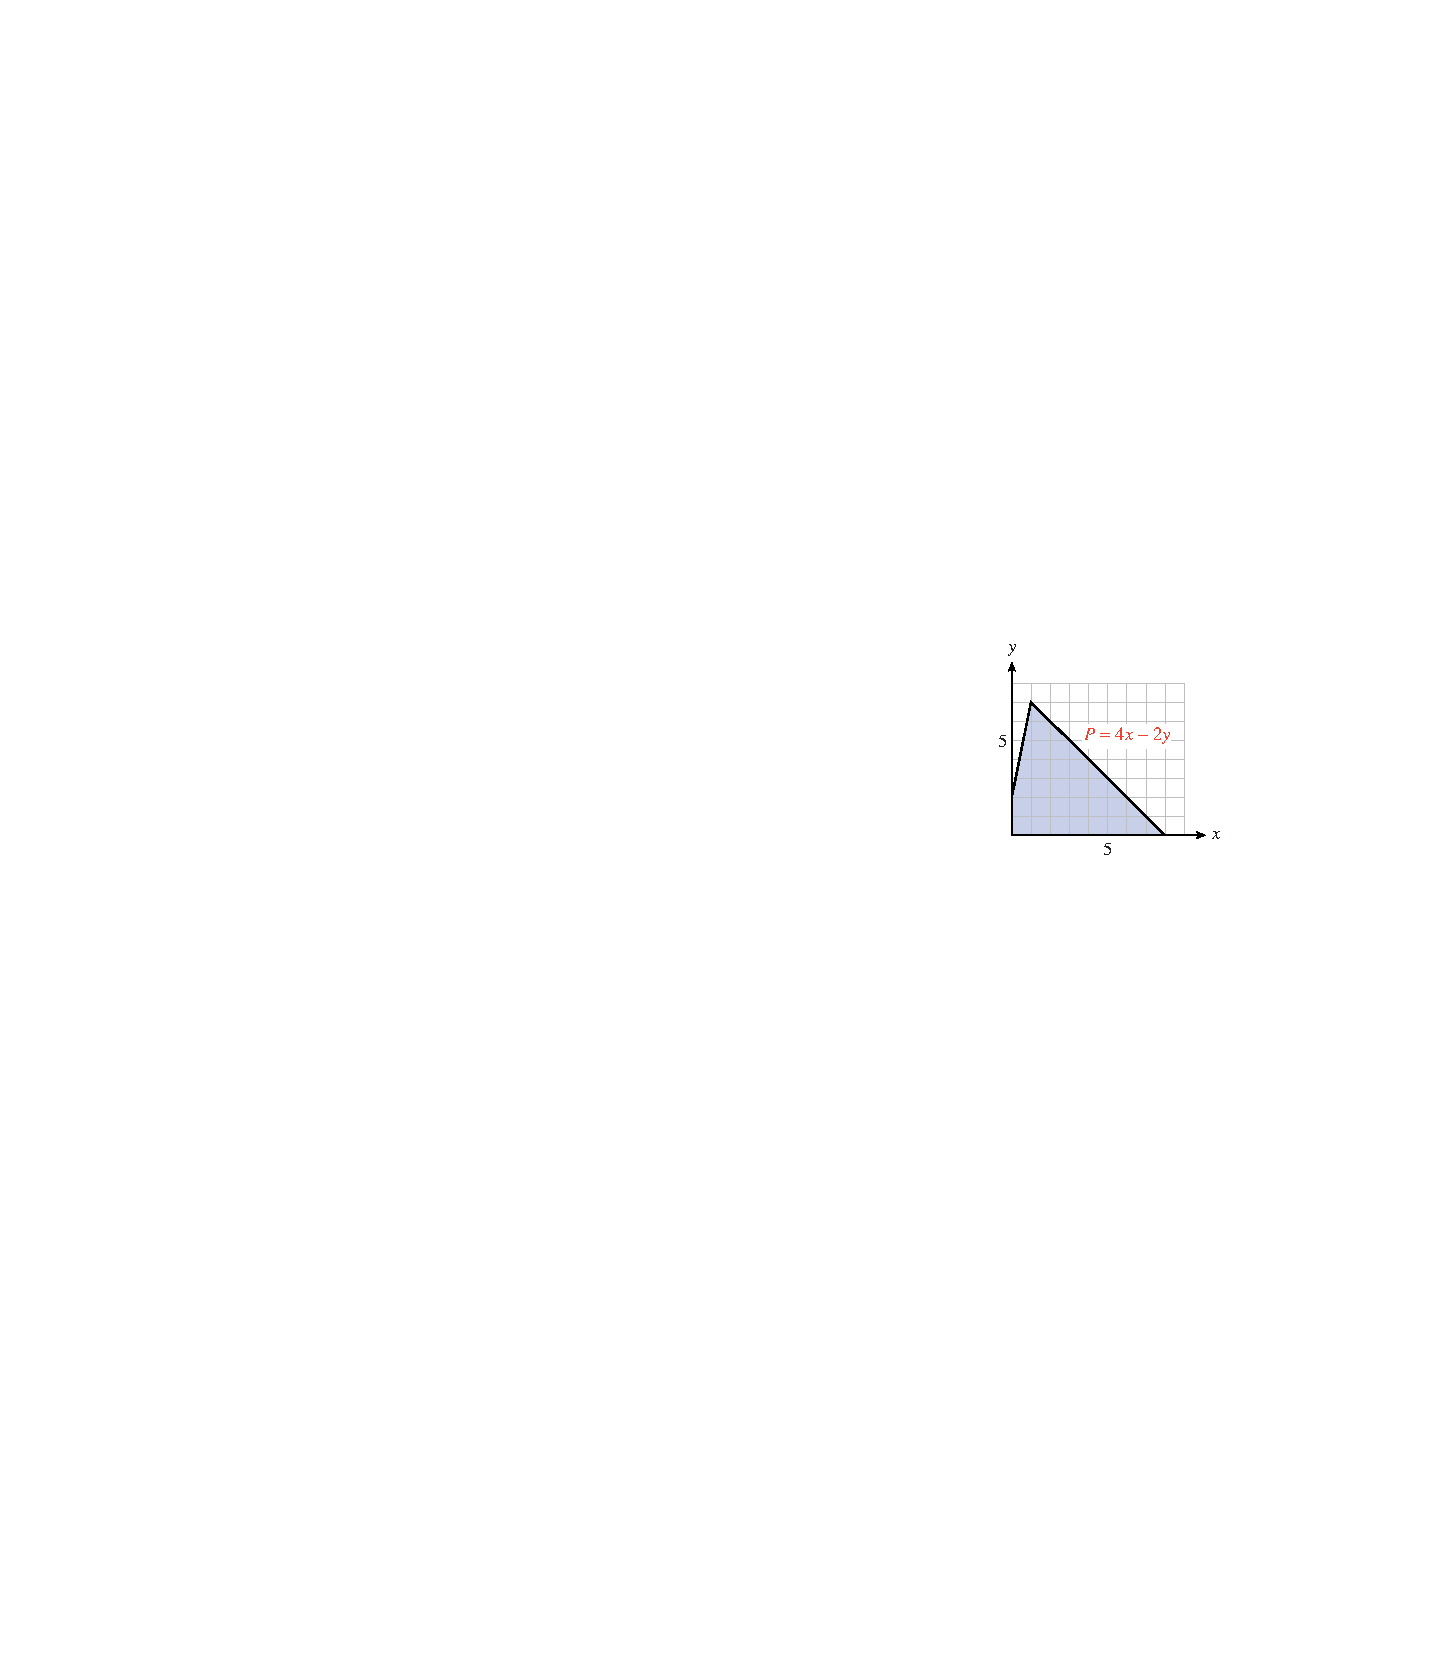
\includegraphics[width=0.35\linewidth]{images/fig-8-5-5}
\end{figure}
%
\begin{exercisegroup}(1)
\exercise[5.]\hypertarget{exercise-9}{}Graph the line that corresponds to a profit of \(\$8\). Find the coordinates of at least one feasible solution that gives a profit of \(\$8\).%
\((2,0) \)%
\exercise[6.]\hypertarget{exercise-10}{}Graph the line that corresponds to a profit of \(\$22\). Find the coordinates of at least one feasible solution that gives a profit of \(\$22\).%
\exercise[7.]\hypertarget{exercise-11}{}\leavevmode%
\begin{enumerate}[label=(\alph*)]
\item\hypertarget{li-52}{}Which line is farther from the origin, the line for a profit of \(\$8\) or the line for the profit of \(\$22\)?%
\item\hypertarget{li-53}{}Use a graph to determine which vertex corresponds to a maximum profit.%
\item\hypertarget{li-54}{}Find the maximum profit.%
\end{enumerate}
%
\leavevmode%
\begin{multicols}{3}
\begin{enumerate}[label=(\alph*)]
\item\hypertarget{li-55}{}\(\$22\)%
\item\hypertarget{li-56}{}\((8, 0)\)%
\item\hypertarget{li-57}{}\(\$32\)%
\end{enumerate}
\end{multicols}
%
\exercise[8.]\hypertarget{exercise-12}{}\leavevmode%
\begin{enumerate}[label=(\alph*)]
\item\hypertarget{li-58}{}Use a graph to determine which vertex corresponds to a minimum profit.%
\item\hypertarget{li-59}{}Find the minimum profit.%
\end{enumerate}
%
\end{exercisegroup}
\par\smallskip\noindent
\hypertarget{exercisegroup-3}{}\par\noindent For Problems 9\textendash{}12, objective functions and the graphs of the feasible solutions are given. \leavevmode%
\begin{enumerate}[label=\alph*]
\item\hypertarget{li-60}{}Use the graph to find the vertex that yields the minimum value of the objective function, and find the minimum value.%
\item\hypertarget{li-61}{}Use the graph to find the vertex that yields the maximum value of the objective function, and find the maximum value.%
\end{enumerate}
%
\begin{exercisegroup}(2)
\exercise[9.]\hypertarget{exercise-13}{}\(C = 3x + y\)\leavevmode%
\begin{figure}
\centering
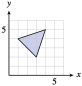
\includegraphics[width=0.7\linewidth]{images/fig-8-5-9}
\end{figure}
%
\par\smallskip
\noindent\textbf{Answer.}\hypertarget{answer-9}{}\quad
\leavevmode%
\begin{multicols}{2}
\begin{enumerate}[label=(\alph*)]
\item\hypertarget{li-62}{}\((1,4) \); \(7\)%
\item\hypertarget{li-63}{}\((4,5) \); \(17\)%
\end{enumerate}
\end{multicols}
%
\exercise[10.]\hypertarget{exercise-14}{}\(C = x + 4y\)\leavevmode%
\begin{figure}
\centering
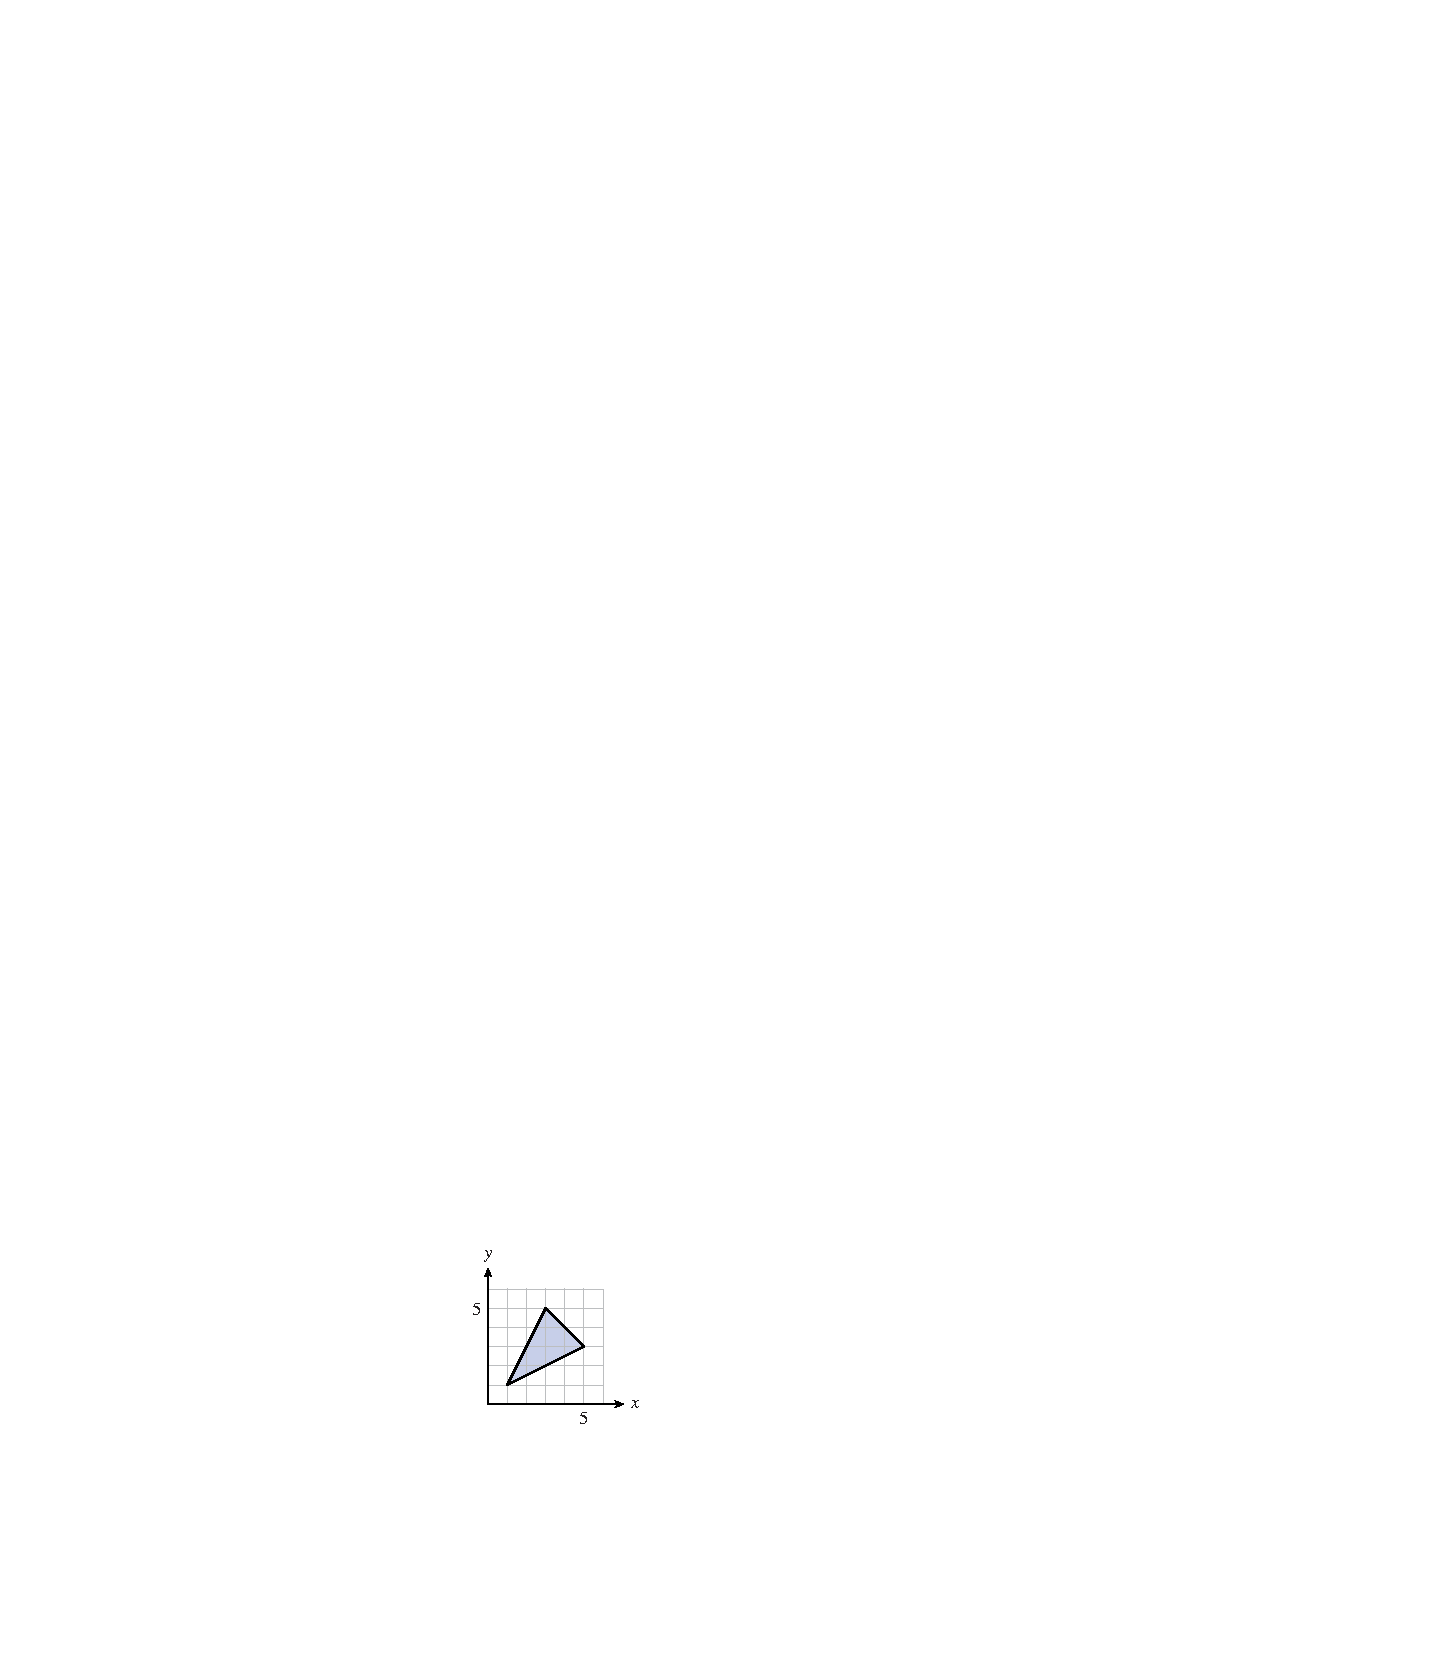
\includegraphics[width=0.7\linewidth]{images/fig-8-5-10}
\end{figure}
%
\exercise[11.]\hypertarget{exercise-15}{}\(C = 5x − 2y\)\leavevmode%
\begin{figure}
\centering
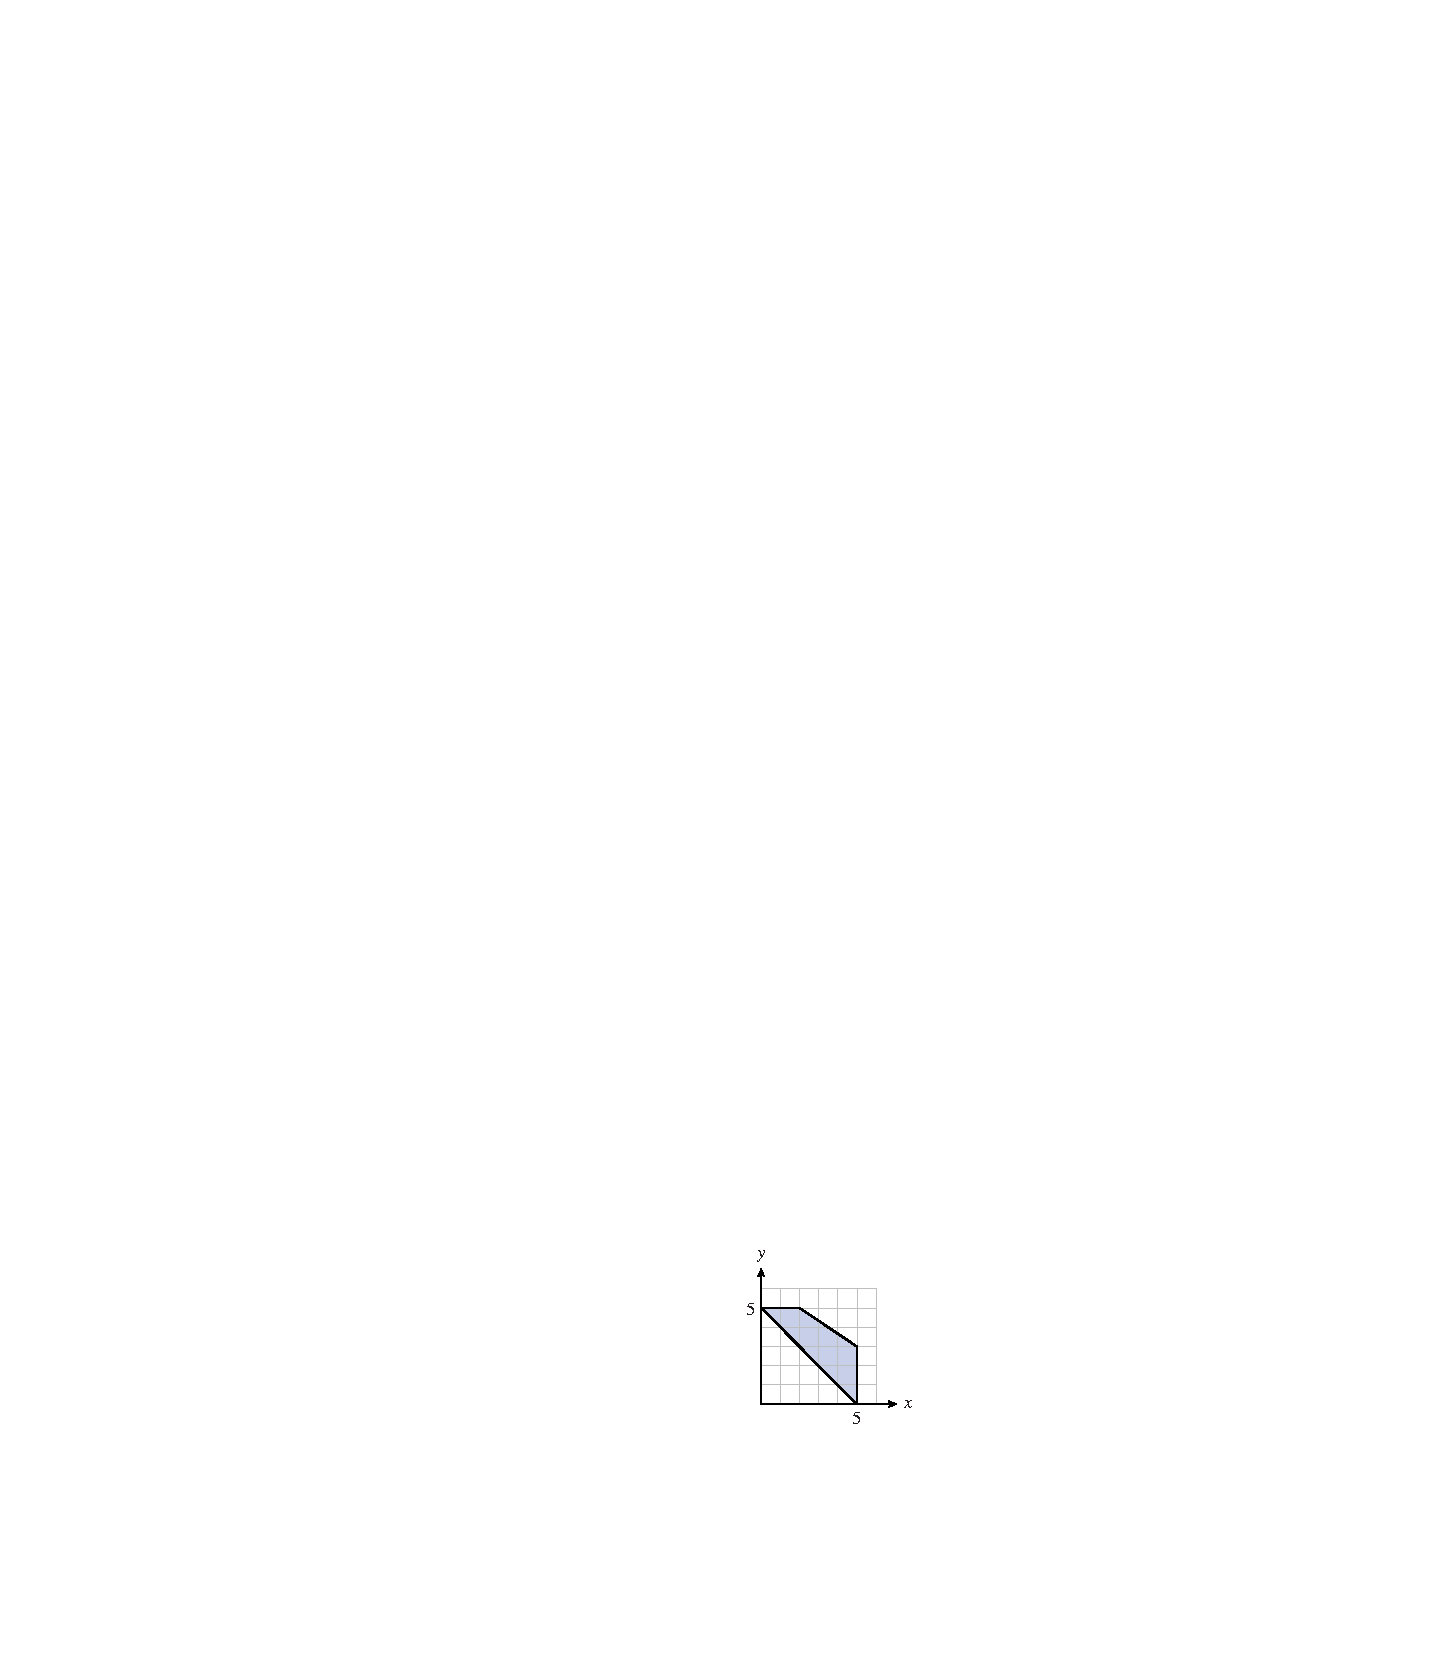
\includegraphics[width=0.7\linewidth]{images/fig-8-5-11}
\end{figure}
%
\par\smallskip
\noindent\textbf{Answer.}\hypertarget{answer-10}{}\quad
\leavevmode%
\begin{multicols}{2}
\begin{enumerate}[label=(\alph*)]
\item\hypertarget{li-64}{}\((0,5) \); \(-10\)%
\item\hypertarget{li-65}{}\((5,0) \); \(25\)%
\end{enumerate}
\end{multicols}
%
\exercise[12.]\hypertarget{exercise-16}{}\(C = 2x − y\)\leavevmode%
\begin{figure}
\centering
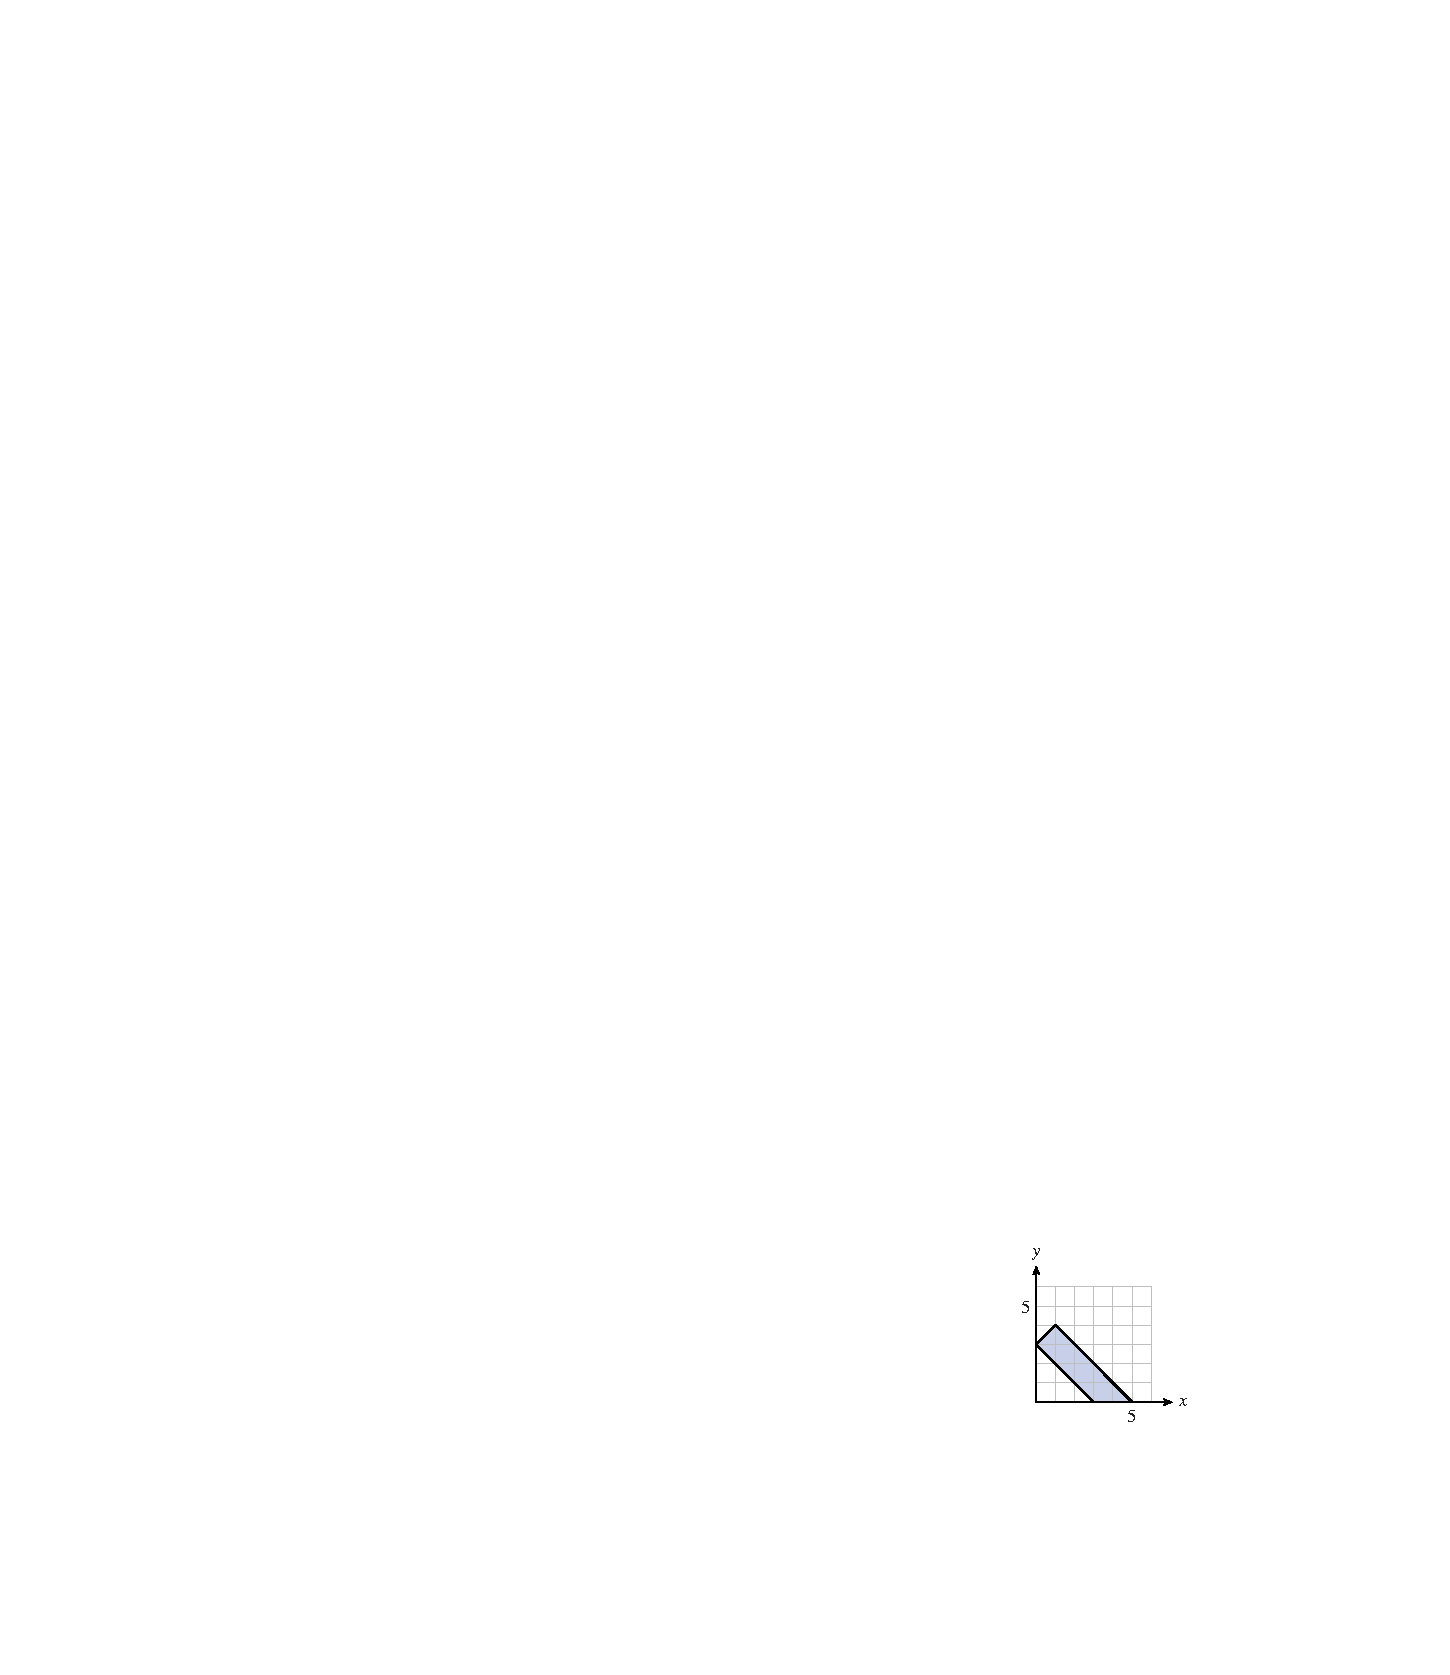
\includegraphics[width=0.7\linewidth]{images/fig-8-5-12}
\end{figure}
%
\end{exercisegroup}
\par\smallskip\noindent
\hypertarget{exercisegroup-4}{}\par\noindent For Problems 13\textendash{}18,\leavevmode%
\begin{enumerate}[label=(\alph*)]
\item\hypertarget{li-66}{}Graph the set of feasible solutions.%
\item\hypertarget{li-67}{}Find the vertex that gives the minimum of the objective function, and find the minimum value.%
\item\hypertarget{li-68}{}Find the vertex that gives the maximum of the objective function, and find the maximum value.%
\end{enumerate}
%
\begin{exercisegroup}(1)
\exercise[13.]\hypertarget{exercise-17}{}Objective function \(C = 3x + 2y\) with constraints \(x\ge 0\), \(y\ge 0\), \(2x + y\le 8\), \(4x + 6y \le 24\)%
\par\smallskip
\noindent\textbf{Answer.}\hypertarget{answer-11}{}\quad
\emph{b.} \((10,0) \); \(0\hphantom{000}\)\emph{c.} \((3,2) \); \(13\)%
\exercise[14.]\hypertarget{exercise-18}{}Objective function \(C = −2x + y\) with constraints \(x\ge 0\), \(y\ge 0\), \(x-2y \ge -10\), \(2x+y\le 10\)%
\exercise[15.]\hypertarget{exercise-19}{}Objective function \(C = 3x − y\) with constraints \(x\ge 0\), \(y\ge 0\), \(x + y\le 14\), \(5x + y \le 50\)%
\par\smallskip
\noindent\textbf{Answer.}\hypertarget{answer-12}{}\quad
\emph{b.} \((0,14) \); \(-14\hphantom{000}\)\emph{c.} \((10,0) \); \(30\)%
\exercise[16.]\hypertarget{exercise-20}{}Objective function \(C = 5x + 4y\) with constraints \(x\ge 0\), \(y\ge 0\), \(2x+y \le 10\), \(x-3y\ge -3\)%
\exercise[17.]\hypertarget{exercise-21}{}Objective function \(C = 200x − 20y\) with constraints \(x\ge 0\), \(y\ge 0\), \(3x + 2y\le 24\), \(x + y \le 9\), \(x + 2y \le 16\)%
\par\smallskip
\noindent\textbf{Answer.}\hypertarget{answer-13}{}\quad
\emph{b.} \((0,8) \); \(-160\hphantom{000}\)\emph{c.} \((8,0) \); \(1600\)%
\exercise[18.]\hypertarget{exercise-22}{}Objective function \(C = 54x + 24y\) with constraints \(x\ge 0\), \(y\ge 0\), \(3x + 2y \le 24\), \(3x-y\le 15\), \(3x − 4y \ge −12\)%
\end{exercisegroup}
\par\smallskip\noindent
\hypertarget{exercisegroup-5}{}\par\noindent For Problems 19\textendash{}26, solve each linear programming problem by graphing. \leavevmode%
\begin{enumerate}[label=\alph*]
\item\hypertarget{li-69}{}Write a formula for the objective function.%
\item\hypertarget{li-70}{}Write a system of inequalities for the constraints.%
\item\hypertarget{li-71}{}Graph the set of feasible solutions.%
\item\hypertarget{li-72}{}Find the optimum solution.%
\end{enumerate}
%
\begin{exercisegroup}(1)
\exercise[19.]\hypertarget{exercise-23}{}The math club is selling tickets for a show by a mathemagician. Student tickets will cost \(\$1\) and faculty tickets will cost \(\$2\). The ticket receipts must be at least \(\$250\) to cover the fee for the performer. An alumna promises to donate one calculator for each student ticket sold and three calculators for each faculty ticket sold. What is the minimum number of calculators that the alumna will donate?%
\par\smallskip
\noindent\textbf{Answer.}\hypertarget{answer-14}{}\quad
\leavevmode%
\begin{multicols}{2}
\begin{enumerate}[label=(\alph*)]
\item\hypertarget{li-73}{}\(C = x + 3y\)%
\item\hypertarget{li-74}{}\(x \ge 0, ~y \ge 0, ~x + 2y \ge 250\)%
\item\hypertarget{li-75}{}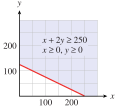
\includegraphics[width=0.8\linewidth]{images/fig-ans-8-4-37}
%
\item\hypertarget{li-76}{}\(250\)%
\end{enumerate}
\end{multicols}
%
\exercise[20.]\hypertarget{exercise-24}{}The math department is having a book sale of unwanted textbooks to raise funds for \(\$300\) in scholarships. Paperback textbooks will be sold for \(\$2\) and the hardcover textbooks will be sold for \(\$5\). If paperback texts weigh \(2\) pounds each and hardcover books weigh \(3\) pounds each, find the minimum weight of textbooks the department must sell in order to raise its required funds.%
\exercise[21.]\hypertarget{exercise-25}{}Jeannette has \(180\) acres of farmland for growing wheat or soy. Each acre of wheat requires two hours of labor at harvest time, and each acre of soy needs one hour of labor. Jeannette will have \(240\) hours of labor available at harvest time. Find the maximum profit Jeannette can make from her two crops if she can get a profit of \(\$36\) per acre for wheat and \(\$24\) per acre for soy.%
\par\smallskip
\noindent\textbf{Answer.}\hypertarget{answer-15}{}\quad
\leavevmode%
\begin{multicols}{2}
\begin{enumerate}[label=(\alph*)]
\item\hypertarget{li-77}{}\(P = 36x + 24y\)%
\item\hypertarget{li-78}{}\(x \ge 0\), \(~y \ge 0\), \(~x + y \le 180\), \(~2x+y\le 240\)%
\item\hypertarget{li-79}{}vertices at \((0,0)\), \((120,0)\), \((60,120)\), \((0,180) \)%
\item\hypertarget{li-80}{}\(\$5040\)%
\end{enumerate}
\end{multicols}
%
\exercise[22.]\hypertarget{exercise-26}{}Vassilis has at most \(\$10,000\) to invest in two banks. Alpha Bank will pay \(6\%\) annual interest and Bank Beta pays \(5\%\) annual interest. Alpha Bank will only insure up to \(\$6000\), so Vassilis will invest no more than that with Alpha. What is the maximum amount of interest Vassilis can earn in \(1\) year?%
\exercise[23.]\hypertarget{exercise-27}{}Gary's pancake recipe includes corn meal and whole wheat flour. Corn meal has \(2.4\) grams of linoleic acid and \(2.5\) milligrams of niacin per cup. Whole wheat flour has \(0.8\) gram of linoleic acid and \(5.2\) milligrams of niacin per cup. These two dry ingredients do not exceed \(3\) cups total. They combine for at least \(3.2\) grams of linoleic acid and at least \(10\) milligrams of niacin. Minimize the number of calories possible in the recipe if corn meal has \(433\) calories per cup and whole wheat flour has \(400\) calories per cup.%
\par\smallskip
\noindent\textbf{Answer.}\hypertarget{answer-16}{}\quad
\leavevmode%
\begin{multicols}{2}
\begin{enumerate}[label=(\alph*)]
\item\hypertarget{li-81}{}\(C = 433x + 400y\)%
\item\hypertarget{li-82}{}\(x \ge 0\), \(~y \ge 0\), \(~2.4x + 0.8y \ge 3.2\), \(~2.5x + 5.2y \ge 10\)%
\item\hypertarget{li-83}{}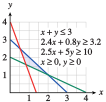
\includegraphics[width=0.8\linewidth]{images/fig-ans-8-4-41}
%
\item\hypertarget{li-84}{}\(967.7\) cal%
\end{enumerate}
\end{multicols}
%
\exercise[24.]\hypertarget{exercise-28}{}Cho requires \(1\) hour of cutting and \(2\) hours of sewing to make a Batman costume. He requires \(2\) hours of cutting and \(1\) hour of sewing to make a Wonder Woman costume. At most \(10\) hours per day are available for cutting and at most \(8\) hours per day are available for sewing. At least one costume must be made each day to stay in business. Find Cho's maximum income from selling one day's costumes if a Batman costume costs \(\$68\) and a Wonder Woman costume costs \(\$76\).%
\end{exercisegroup}
\par\smallskip\noindent
\hypertarget{exercisegroup-6}{}\par\noindent For Problems 25\textendash{}30, use a graphing calculator to find approximate values for the maximum and minimum of the objective function.%
\begin{exercisegroup}(1)
\exercise[25.]\hypertarget{exercise-29}{}Objective function \(C = 8.7x − 4.2y\) with constraints \(x \ge 0\), \(y \ge 0\), \(1.7x − 4.5y \ge −9\), \(14.3x + 10.9y\le 28.6\)%
\par\smallskip
\noindent\textbf{Answer.}\hypertarget{answer-17}{}\quad
Maximum \(17.4\); minimum \(−8.4\)%
\exercise[26.]\hypertarget{exercise-30}{}Objective function \(C = −142x + 83y\) with constraints \(x \ge 0\), \(y \ge 0\), \(21x − 49y \ge −147\), \(19x + 21y\le 171\)%
\exercise[27.]\hypertarget{exercise-31}{}Objective function \(C = 312x + 92y\) with constraints \(x \ge 0\), \(y \ge 0\), \(18x + 17y \le 284\), \(51x + 11y\le 656\)%
\par\smallskip
\noindent\textbf{Answer.}\hypertarget{answer-18}{}\quad
Maximum \(4112\); minimum \(0\)%
\exercise[28.]\hypertarget{exercise-32}{}Objective function \(C = 5.3x + 4.2y\) with constraints \(x \ge 0\), \(y \ge 0\), \(2.5x + 1.7y \le 20.1\), \(0.09x − 0.31y \ge −0.39\)%
\exercise[29.]\hypertarget{exercise-33}{}Objective function \(C = 38x + 24y \le 294\), \(35x + 34y \le 310\), \(13x + 29y \le 197\)%
\par\smallskip
\noindent\textbf{Answer.}\hypertarget{answer-19}{}\quad
Maximum \(1908\); minimum \(0\)%
\exercise[30.]\hypertarget{exercise-34}{}Objective function \(C = 54x + 24y\) with constraints \(x \ge 0\), \(y \ge 0\), \(43x + 32y \le 333\), \(23x − 9y \le 152\), \(73x − 94y\ge −296\)%
\end{exercisegroup}
\par\smallskip\noindent
%
%% A lineskip in table of contents as transition to appendices, backmatter
\addtocontents{toc}{\vspace{\normalbaselineskip}}
%
%
\appendix
%
\typeout{************************************************}
\typeout{Appendix A Algebra Skills Refresher}
\typeout{************************************************}
\chapter[{Algebra Skills Refresher}]{Algebra Skills Refresher}\label{appendix-a}
\typeout{************************************************}
\typeout{Section A.1 Numbers and Operations}
\typeout{************************************************}
\section[{Numbers and Operations}]{Numbers and Operations}\label{Numbers-and-Operations}
\typeout{************************************************}
\typeout{Subsection A.1.1 Order of Operations}
\typeout{************************************************}
\subsection[{Order of Operations}]{Order of Operations}\label{Order-of-Operations}
Numerical calculations often involve more than one operation. So that everyone agrees on how such expressions should be evaluated, we follow the order of operations.%
\begin{assemblage}{Order of Operations}\label{assemblage-3}
\leavevmode%
\begin{enumerate}[label=*\arabic**]
\item\hypertarget{li-85}{}Simplify any expressions within grouping symbols (parentheses, brackets, square root bars, or fraction bars). Start with the innermost grouping symbols and work outward.%
\item\hypertarget{li-86}{}Evaluate all powers and roots.%
\item\hypertarget{li-87}{}Perform multiplications and divisions in order from left to right.%
\item\hypertarget{li-88}{}Perform additions and subtractions in order from left to right.%
\end{enumerate}
%
\end{assemblage}
\typeout{************************************************}
\typeout{Subsection A.1.2 Parentheses and Fraction Bars}
\typeout{************************************************}
\subsection[{Parentheses and Fraction Bars}]{Parentheses and Fraction Bars}\label{subsection-6}
We can use parentheses to override the multiplication-first rule. Compare the two expressions below.%
\begin{align*}
\amp\text{The sum of 4 times 6 and 10} \amp\amp 4 \cdot 6 + 10\\
\amp\text{4 times the sum of 6 and 10} \amp\amp  4(6 + 10)
\end{align*}
%
\par
In the first expression, we perform the multiplication \(4\times 6\) first, but in the second expression we perform the addition \(6 + 10\) first, because it is enclosed in parentheses.%
\par
The location (or absence) of parentheses can drastically alter the meaning of an expression. In the following example, note how the location of the parentheses changes the value of the expression.%
\begin{example}[]\label{example-parentheses}
\leavevmode%
\begin{enumerate}[label=*\alph**]
\item\hypertarget{li-89}{}\(\begin{aligned}5-3\cdot 4^2 \amp = 5-3\cdot 16\\
\amp = 5-48=-43
\end{aligned}                \)%
\item\hypertarget{li-90}{}\(\begin{aligned}5-(3\cdot 4)^2 \amp = 5-12^2\\
\amp= 5-144 = -139
\end{aligned}\)%
\item\hypertarget{li-91}{}\(\begin{aligned}(5-3\cdot 4)^2 \amp = (5-12)^2\\
\amp = (-7)^2 = 49
\end{aligned}\)%
\item\hypertarget{li-92}{}\(\begin{aligned}(5-3)\cdot 4^2 \amp = 2\cdot 16\\
\amp = 32
\end{aligned}\)%
\end{enumerate}
%
\end{example}
\begin{warning}[]\label{warning-1}
In the expression \(5 − 12^2\), which appears in \hyperref[example-parentheses]{Example~\ref{example-parentheses}}, the exponent \(2\) applies only to \(12\), not to \(-12\). Thus, \(5 − 12^2 \ne 5 + 144\).%
\end{warning}
\par
The order of operations mentions other grouping devices besides parentheses: fraction bars and square root bars. Notice how the placement of the fraction bar affects the expressions in the next example.%
\begin{example}[]\label{example-6}
\leavevmode%
\begin{enumerate}[label=*\alph**]
\item\hypertarget{li-93}{}\(\begin{aligned}
\frac{1+2}{3\cdot 4} \amp = \frac{3}{12}\\
\amp = \frac{1}{4}
\end{aligned}\)%
\item\hypertarget{li-94}{}\(\begin{aligned}
1+\frac{2}{3\cdot 4} \amp = 1+ \frac{2}{12}\\
\amp = 1+\frac{1}{6}=\frac{7}{6}
\end{aligned}                \)%
\item\hypertarget{li-95}{}\(\begin{aligned}
\frac{1+2}{3}\cdot 4 \amp = \frac{3}{3}\cdot 4\\
\amp = 1\cdot 4=4
\end{aligned}\)%
\item\hypertarget{li-96}{}\(\begin{aligned}
1+\frac{2}{3}\cdot 4 \amp = 1+ \frac{8}{3}\\
\amp = \frac{3}{3}+\frac{8}{3}=\frac{11}{3}
\end{aligned}                \)%
\end{enumerate}
%
\end{example}
\typeout{************************************************}
\typeout{Subsection A.1.3 Radicals}
\typeout{************************************************}
\subsection[{Radicals}]{Radicals}\label{subsection-7}
You are already familiar with square roots. Every nonnegative number has two square roots, defined as follows:%
\begin{equation*}
s ~~\text{ is a square root of }~~ n ~~\text{ if }~~s^2 = n
\end{equation*}
There are several other kinds of roots, one of which is called the \terminology{cube root}, denoted by \(\sqrt[3]{n}\). We define the cube root as follows.%
\begin{assemblage}{Cube Roots}\label{assemblage-4}
%
\begin{equation*}
b ~~\text{ is a cube root of }~~~ n ~~~\text{ if }~~~ b ~\text{ cubed equals }~~n.
\end{equation*}
In symbols, we write%
\begin{equation*}
b=\sqrt[3]{n} ~~\text{ if } ~~ b^3=n
\end{equation*}
%
\end{assemblage}
\par
Although we cannot take the square root of a \emph{negative number}, we can take the \emph{cube root} of \emph{any} real number. For example,%
\begin{equation*}
\sqrt[3]{64}=4 ~~\text{ because }~~ 4^3=64
\end{equation*}
and%
\begin{equation*}
\sqrt[3]{-27}=-3 ~~\text{ because }~~ (-3)^3=-27
\end{equation*}
%
\par
In the order of operations, simplifying radicals and powers comes after parentheses but before products and quotients.%
\begin{example}[]\label{example-7}
Simplify each expression. \leavevmode%
\begin{enumerate}[label=*\alph**]
\item\hypertarget{li-97}{}\(3\sqrt[3]{-8}\)%
\item\hypertarget{li-98}{}\(2-\sqrt[3]{-125}\)%
\item\hypertarget{li-99}{}\(\displaystyle{\frac{6-\sqrt[3]{-27}}{2}}\)%
\end{enumerate}
%
\par\medskip\noindent%
\textbf{Solution.}\quad \leavevmode%
\begin{enumerate}[label=*\alph**]
\item\hypertarget{li-100}{}\(3\sqrt[3]{-8}=3(-2)=-6\)%
\item\hypertarget{li-101}{}\(2-\sqrt[3]{-125}=2-(-5)=7\)%
\item\hypertarget{li-102}{}\(\displaystyle{\frac{6-\sqrt[3]{-27}}{2}=\frac{6-(-3)}{2}=\frac{9}{2}}\)%
\end{enumerate}
%
\end{example}
\typeout{************************************************}
\typeout{Subsection A.1.4 Scientific Notation}
\typeout{************************************************}
\subsection[{Scientific Notation}]{Scientific Notation}\label{Scientific-Notation}
Scientists and engineers regularly encounter very large numbers such as%
\begin{equation*}
5,980,000,000,000,000,000,000,000
\end{equation*}
(the mass of the Earth in kilograms) and very small numbers such as%
\begin{equation*}
0.000 \,000 \,000 \,000 \,000 \,000 \,000 \,001 \,67
\end{equation*}
(the mass of a hydrogen atom in grams). These numbers can be written in a more compact and useful form by using powers of \(10\).%
\par
In our base \(10\) number system, multiplying a number by a positive power of \(10\) has the effect of moving the decimal place \(k\) places to the right, where \(k\) is the exponent in the power of \(10\). For example,%
\begin{equation*}
3.529 \times 10^2 = 352.9 ~~~\text{ and }~~~ 25 \times 104 = 250,000
\end{equation*}
Multiplying by a power of \(10\) with a negative exponent moves the decimal place to the left. For example,%
\begin{equation*}
1728 \times 10^{−3} = 1.728 ~~~\text{ and }~~~ 4.6 \times 10^{−5} = 0.000046
\end{equation*}
%
\par
Using this property, we can write any number as the product of a number between \(1\) and \(10\) (including \(1\)) and a power of \(10\). For example, the mass of the Earth and the mass of a hydrogen atom can be expressed as%
\begin{equation*}
5.98 \times 1024 \text{ kilograms}\hphantom{blank} \text{ and }\hphantom{blank}1.67 \times 10^{−24} \text{ gram}
\end{equation*}
respectively. A number written in this form is said to be expressed in \terminology{scientific notation}.%
\begin{assemblage}{To Write a Number in Scientific Notation:}\label{assemblage-5}
\leavevmode%
\begin{enumerate}[label=*\arabic**]
\item\hypertarget{li-103}{}Locate the decimal point so that there is exactly one nonzero digit to its left.%
\item\hypertarget{li-104}{}Count the number of places you moved the decimal point: This determines the power of \(10\). %
\begin{enumerate}[label=*\alph**]
\item\hypertarget{li-105}{}If the original number is greater than \(10\), the exponent is positive.%
\item\hypertarget{li-106}{}If the original number is less than \(1\), the exponent is negative.%
\end{enumerate}
%
\end{enumerate}
%
\end{assemblage}
\begin{example}[]\label{example-8}
Write each number in scientific notation. \leavevmode%
\begin{enumerate}[label=*\alph**]
\item\hypertarget{li-107}{}\(\begin{aligned}
478,000 \amp = 4.78000 \times 10^5\\
\amp = 4.78 \times 10^5
\end{aligned}\)%
\item\hypertarget{li-108}{}\(\begin{aligned}
0.00032 \amp= 00003.2 \times 10^{−4}\\
\amp = 3.2 \times 10^{-4}
\end{aligned}\)%
\end{enumerate}
%
\end{example}
\begin{example}[]\label{example-9}
The average American eats \(110\) kilograms of meat per year. It takes about \(16\) kilograms of grain to produce \(1\) kilogram of meat, and advanced farming techniques can produce about \(6000\) kilograms of grain on each hectare of arable land. (The hectare is \(10,000\) square meters, or just under \(2 1⁄2\) acres.) Now, the total land area of the Earth is about \(13\) billion hectares, but only about \(11\%\) of that land is arable. Is it possible for each of the \(5.5\) billion people on Earth to eat as much meat as Americans do?%
\par\medskip\noindent%
\textbf{Solution.}\quad First we will compute the amount of meat necessary to feed every person on Earth \(110\) kilograms per year. There are \(5.5 \times 10^9\) people on Earth.%
\begin{equation*}
(5.5\times 10^9 \text{ people})\times (110 \text{ kg/person}) = 6.05\times 10^{11} \text{ kg of meat}
\end{equation*}
Next we will compute the amount of grain needed to produce that much meat.%
\begin{equation*}
(16 \text{ kg of grain/kg of meat})\times (6.05\times 10^{11} \text{ kg of meat}) = 9.68\times 10^{12} \text{ kg of grain}
\end{equation*}
Next we will see how many hectares of land are needed to produce that much grain.%
\begin{equation*}
(9.68\times 10^{12} \text{ kg of grain})\div(6000 \text{ kg/hectare}) = 1.613\times 10^9 \text{ hectares}
\end{equation*}
Finally, we will compute the amount of arable land available for grain production.%
\begin{equation*}
0.11\times (13\times 10^9 \text{ hectares}) = 1.43\times 10^9 \text{ hectares}
\end{equation*}
Thus, even if we use every hectare of arable land to produce grain for livestock, we will not have enough to provide every person on Earth with \(110\) kilograms of meat per year.%
\end{example}
\typeout{************************************************}
\typeout{Section A.2 Linear Equations and Inequalities}
\typeout{************************************************}
\section[{Linear Equations and Inequalities}]{Linear Equations and Inequalities}\label{appendix-Linear-Equations-and-Inequalities}
An \terminology{equation} is just a mathematical statement that two expressions are equal. Equations relating two variables are particularly useful. If we know the value of one of the variables, we can find the corresponding value of the other variable by solving the equation.%
\begin{example}[]\label{example-10}
The equation \(w = 6h\) gives Loren's wages, \(w\), in terms of the number of hours she works, \(h\). How many hours does Loren need to work next week if she wants to earn \(\$225\)?%
\par\medskip\noindent%
\textbf{Solution.}\quad We know that \(w = 225\), and we would like to know the value of \(h\). We substitute the value for \(w\) into our equation and then solve for \(h\).%
\begin{align*}
w \amp= 6h\amp\amp \text{Substitute 225 for }w.\\
\alert{225} \amp= 6h\amp\amp \text{Divide both sides by } 6.\\
\frac{225}{\alert{6}}\amp = \frac{6h}{\alert{6}}\amp\amp \text{Simplify.}\\
375.5\amp = h
\end{align*}
Loren must work \(37.5\) hours in order to earn \(\$225\). In reality, Loren will probably have to work for \(38\) hours, because most employers do not pay for portions of an hour's work. Thus, Loren needs to work for \(38\) hours.%
\end{example}
\par
To solve an equation we can generate simpler equations that have the same solutions. Equations that have identical solutions are called \terminology{equivalent equations}. For example,%
\begin{equation*}
3x − 5 = x + 3
\end{equation*}
and%
\begin{equation*}
2x = 8
\end{equation*}
are equivalent equations because the solution of each equation is \(4\). Often we can find simpler equivalent equations by undoing in reverse order the operations performed on the variable.%
\typeout{************************************************}
\typeout{Subsection A.2.1 Solving Linear Equations}
\typeout{************************************************}
\subsection[{Solving Linear Equations}]{Solving Linear Equations}\label{subsection-9}
\terminology{Linear}, or first-degree, equations can be written so that every term is either a constant or a constant times the variable. The equations above are examples of linear equations. Recall the following rules for solving linear equations.%
\begin{assemblage}{To Generate Equivalent Equations}\label{assemblage-6}
\leavevmode%
\begin{enumerate}[label=*\arabic**]
\item\hypertarget{li-109}{}We can add or subtract the \emph{same} number on \emph{both} sides of an equation.%
\item\hypertarget{li-110}{}We can multiply or divide \(both\) sides of an equation by the \(same\) number (except zero).%
\end{enumerate}
%
\end{assemblage}
\par
Applying either of these rules produces a new equation equivalent to the old one and thus preserves the solution.We use the rules to isolate the variable on one side of the equation.%
\begin{example}[]\label{example-11}
Solve the equation \(3x − 5 = x + 3\).%
\par\medskip\noindent%
\textbf{Solution.}\quad We first collect all the variable terms on one side of the equation, and the constant terms on the other side.%
\begin{align*}
3x − 5 \alert{{}− x} \amp = x + 3 \alert{{}− x}\amp\amp \text{Subtract }x \text{ from both sides.}
\\
2x − 5 \amp = 3\amp\amp \text{Simplify.}
\\
2x − 5 \alert{{}+ 5} \amp = 5 \alert{{}+ 5}\amp\amp \text{Add 5 to both sides.}
\\
2x \amp = 8 \amp\amp\text{Simplify.}
\\
\frac{2x}{\alert{2}}\amp =\frac{8}{\alert{2}}\amp\amp\text{Divide both sides by 2.}
\\
x\amp = 4\amp\amp\text{Simplify.}
\end{align*}
The solution is \(4\). (You can check the solution by substituting \(4\) into the original equation to show that a true statement results.)%
\end{example}
\par
The following steps should enable you to solve any linear equation. Of course, you may not need all the steps for a particular equation.%
\begin{assemblage}{To Solve a Linear Equation:}\label{assemblage-7}
\leavevmode%
\begin{enumerate}[label=*\arabic**]
\item\hypertarget{li-111}{}Simplify each side of the equation separately. %
\begin{enumerate}[label=*\alph**]
\item\hypertarget{li-112}{}Apply the distributive law to remove parentheses.%
\item\hypertarget{li-113}{}Collect like terms.%
\end{enumerate}
%
\item\hypertarget{li-114}{}By adding or subtracting appropriate terms to both sides of the equation, get all the variable terms on one side and all the constant terms on the other.%
\item\hypertarget{li-115}{}Divide both sides of the equation by the coefficient of the variable.%
\end{enumerate}
%
\end{assemblage}
\begin{example}[]\label{example-12}
Solve \(3(2x − 5) − 4x = 2x − (6 − 3x)\).%
\par\medskip\noindent%
\textbf{Solution.}\quad We begin by simplifying each side of the equation.%
\begin{align*}
3(2x − 5) − 4x \amp = 2x − (6 − 3x) \amp\amp\text{Apply the distributive law.}
\\
6x − 15 − 4x \amp= 2x − 6 + 3x \amp\amp\text{Combine like terms on each side.}
\\
2x − 15 \amp= 5x − 6
\end{align*}
Next, we collect all the variable terms on the left side of the equation, and all the constant terms on the right side.%
\begin{align*}
2x − 15 − 5x + 15 \amp= 5x − 6 − 5x + 15 \amp\amp\text{Add }−5x + 15 \text{ to both sides.}
\\
−3x \amp= 9
\end{align*}
Finally, we divide both sides of the equation by the coefficient of the variable.%
\begin{align*}
−3x \amp= 9 \amp\amp\text{Divide both sides by }−3.
\\
x \amp =-3
\end{align*}
The solution is \(−3\).%
\end{example}
\typeout{************************************************}
\typeout{Subsection A.2.2 Formulas}
\typeout{************************************************}
\subsection[{Formulas}]{Formulas}\label{subsection-10}
A \terminology{formula} is an equation that relates several variables. For example, the equation%
\begin{equation*}
P = 2l + 2w
\end{equation*}
gives the perimeter of a rectangle in terms of its length and width.%
\par
Suppose we have some wire fence to enclose an exercise area for rabbits, and we would like to see what dimensions are possible for different rectangles with that perimeter. In this case, it would be more useful to have a formula for the length of the rectangle in terms of its perimeter and its width. We can find such a formula by solving the perimeter formula for \(l\) in terms of \(P\) and \(w\).%
\begin{align*}
2l + 2w \amp= P \amp\amp\text{Subtact }2 w \text{ from both sides.}\\
2l \amp= P − 2w \amp\amp\text{Divide both sides by 2.}\\
l \amp= \frac{P − 2w}{2}
\end{align*}
The result is a new formula that gives the length of a rectangle in terms of its perimeter and its width.%
\begin{example}[]\label{example-13}
The formula \(5F = 9C + 160\) relates the temperature in degrees Fahrenheit, \(F\), to the temperature in degrees Celsius, \(C\). Solve the formula for \(C\) in terms of \(F\).%
\par\medskip\noindent%
\textbf{Solution.}\quad We begin by isolating the term that contains \(C\).%
\begin{align*}
5F \amp= 9C + 160 \amp\amp\text{Subtract 160 from both sides.}
\\
5F − 160 \amp = 9C \amp\amp\text{Divide both sides by 9.}
\\
\frac{5F − 160}{9} \amp =C
\end{align*}
We can also write the formula for \(C\) in terms of \(F\) as \(C = \frac{5}{9}F − \frac{160}{9}\).%
\end{example}
\begin{example}[]\label{example-14}
Solve \(3x − 5y = 40\) for \(y\) in terms of \(x\).%
\par\medskip\noindent%
\textbf{Solution.}\quad We isolate \(y\) on one side of the equation.%
\begin{align*}
3x − 5y \amp = 40\amp\amp\text{Subtract }3x \text{ from both sides.}
\\
−5y \amp = 40 − 3x\amp\amp\text{Divide both sides by }-5.
\\
\frac{−5y}{-5} \amp = \frac{40 − 3x}{-5}\amp\amp\text{Simplify both sides.}               
\\
y \amp = −8 + \frac{3}{5}x
\end{align*}
%
\end{example}
\typeout{************************************************}
\typeout{Subsection A.2.3 Linear Inequalities}
\typeout{************************************************}
\subsection[{Linear Inequalities}]{Linear Inequalities}\label{subsection-11}
The symbol \(\gt\) is called an \terminology{inequality symbol}, and the statement \(a\gt b\) is called an \terminology{inequality}. There are four inequality symbols:%
\begin{align*}
\amp\gt \amp\amp\text{is greater than}\\
\amp\lt \amp\amp\text{is less than}\\
\amp\ge \amp\amp\text{is greater than or equal to}\\
\amp\le \amp\amp\text{is less than or equal to}
\end{align*}
%
\par
Inequalities that include the symbols \(\gt\) or \(\le\) are called \terminology{strict inequalities}; those that include \(\ge\) or \(\le\) are called \terminology{nonstrict}.%
\par
If we multiply or divide both sides of an inequality by a negative number, the direction of the inequality must be reversed. For example, if we multiply both sides of the inequality%
\begin{equation*}
2\lt 5
\end{equation*}
by \(−3\), we get%
\begin{align*}
\alert{−3}(2) \amp\gt \alert{−3}(5)\amp\amp \text{Change inequality symbol from }\lt \text{ to }\gt.\\
−6 \amp\gt −15.
\end{align*}
Because of this property, the rules for solving linear equations must be revised slightly for solving linear inequalities.%
\begin{assemblage}{To Solve a Linear Inequality:}\label{assemblage-8}
\leavevmode%
\begin{enumerate}[label=*\arabic**]
\item\hypertarget{li-116}{}We may add or subtract the same number to both sides of an inequality without changing its solutions.%
\item\hypertarget{li-117}{}We may multiply or divide both sides of an inequality by a \emph{positive} number without changing its solutions.%
\item\hypertarget{li-118}{}If we multiply or divide both sides of an inequality by a \emph{negative} number, we must \emph{reverse the direction of the inequality symbol}.%
\end{enumerate}
%
\end{assemblage}
\begin{example}[]\label{example-15}
Solve the inequality \(4 − 3x \ge −17\).%
\par\medskip\noindent%
\textbf{Solution.}\quad Use the rules above to isolate \(x\) on one side of the inequality.%
\begin{align*}
4 − 3x \amp\ge −17\amp\amp\text{Subtract 4 from both sides.}
\\
−3x \amp\ge −21\amp\amp\text{Divide both sides by }−3.
\\
x \amp\le 7
\end{align*}
Notice that we reversed the direction of the inequality when we divided by \(-3\). Any number less than or equal to \(7\) is a solution of the inequality.%
\end{example}
\par
A \terminology{compound inequality} involves two inequality symbols.%
\begin{example}[]\label{example-compound-inequality}
Solve \(4 \le 3x + 10 \le 16\).%
\par\medskip\noindent%
\textbf{Solution.}\quad We isolate \(x\) by performing the same operations on all three sides of the inequality.%
\begin{alignat*}{3}
4 \amp{}\le{} 3x\amp {}+{}\amp 10 \amp{}\le{} 16\hphantom{blank} \amp\text{Subtract }10.
\\
−6 \amp{}\le{} \amp 3x\amp {}{}\amp {}\le{} 6\hphantom{blank} \amp\text{Divide by }3.
\\
−2 \amp{}\le{} \amp x\amp {}{}\amp{}\le{} 2\hphantom{blank}\amp
\end{alignat*}
The solutions are all numbers between \(-2\) and \(2\), inclusive.%
\end{example}
\typeout{************************************************}
\typeout{Subsection A.2.4 Interval Notation}
\typeout{************************************************}
\subsection[{Interval Notation}]{Interval Notation}\label{subsection-12}
The solutions of the inequality in \hyperref[example-compound-inequality]{Example~\ref{example-compound-inequality}} form an interval. An \terminology{interval} is a set that consists of all the real numbers between two numbers \(a\) and \(b\).%
\par
The set \(−2 \le x \le 2\) includes its endpoints \(-2\) and \(2\), so we call it a \terminology{closed interval}, and we denote it by \([−2, 2]\) (see \hyperref[fig-numline-closed-vs-open]{Figure~\ref{fig-numline-closed-vs-open}}a). The square brackets tell us that the endpoints are included in the interval. An interval that does not include its endpoints, such as \(−2 \lt x \lt 2\), is called an \terminology{open interval}, and we denote it with round brackets, \((−2, 2)\) (see \hyperref[fig-numline-closed-vs-open]{Figure~\ref{fig-numline-closed-vs-open}}b). \leavevmode%
\begin{figure}
\centering
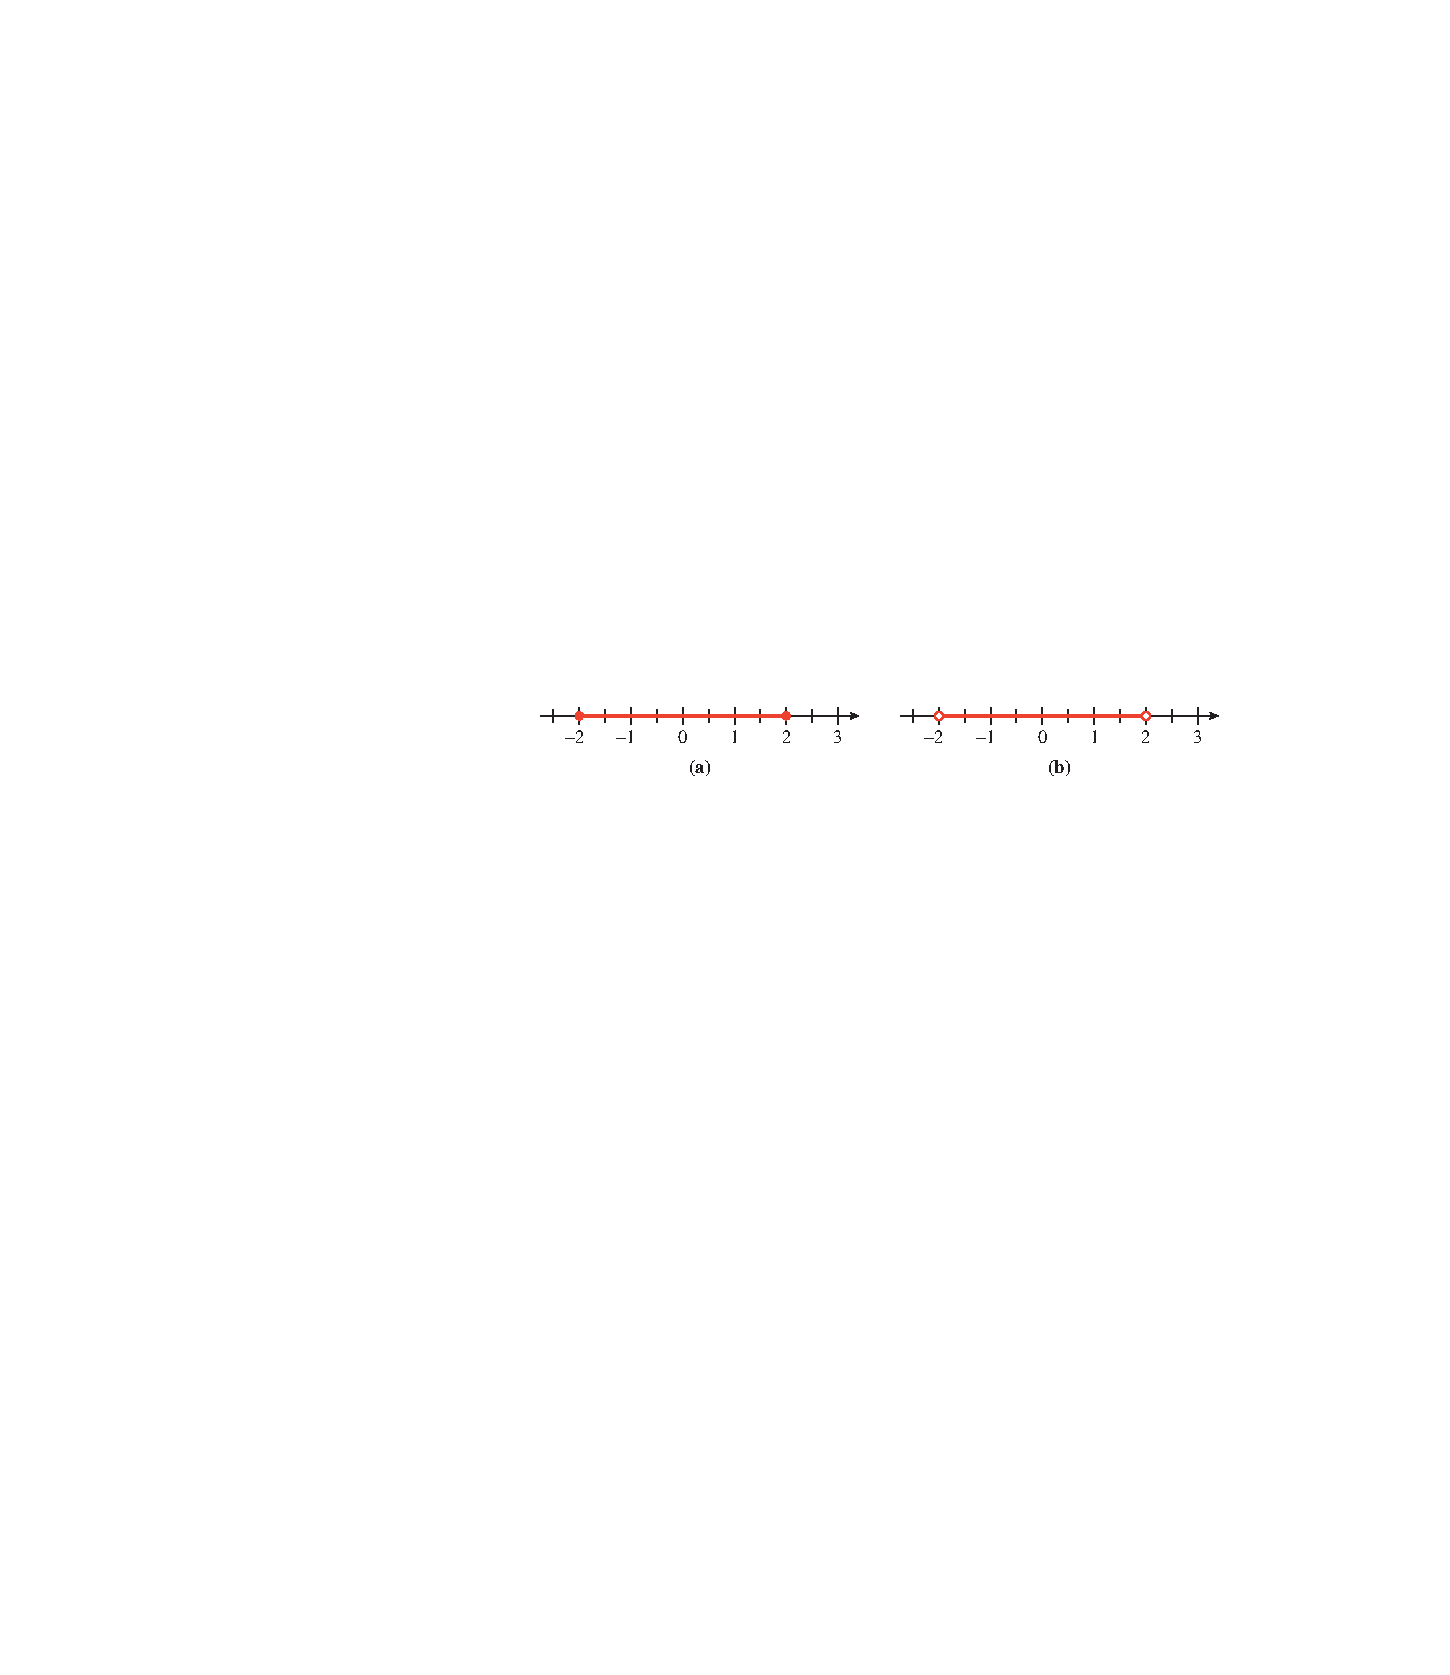
\includegraphics[width=1\linewidth]{images/fig-numline-closed-vs-open}
\caption{\label{fig-numline-closed-vs-open}}
\end{figure}
%
\begin{warning}[]\label{warning-2}
Do not confuse the open interval \((−2, 2)\) with the point \((−2, 2)\)! The notation is the same, so you must decide from the context whether an interval or a point is being discussed.%
\end{warning}
\par
We can also discuss \terminology{infinite intervals}, such as \(x\lt 3\) and \(x\ge -1\), shown in \hyperref[fig-numline-infinite-intervals]{Figure~\ref{fig-numline-infinite-intervals}}. We denote the interval \(x\lt 3\) by \((−\infty, 3)\), and the interval \(x\ge -1\) by \([−1, \infty)\). The symbol \(\infty\), for infinity, does not represent a specific real number; it indicates that the interval continues forever along the real line. \leavevmode%
\begin{figure}
\centering
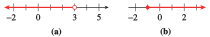
\includegraphics[width=1\linewidth]{images/fig-numline-infinite-intervals}
\caption{\label{fig-numline-infinite-intervals}}
\end{figure}
%
\par
Finally, we can combine two or more intervals into a larger set. For example, the set consisting of \(x\lt -1\) or \(x\gt 2\), shown in \hyperref[fig-numline-disjoint-infinite-intervals]{Figure~\ref{fig-numline-disjoint-infinite-intervals}}, is the \terminology{union} of two intervals and is denoted by \((−\infty,−2) \cup (2,\infty)\). \leavevmode%
\begin{figure}
\centering
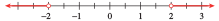
\includegraphics[width=1\linewidth]{images/fig-numline-disjoint-infinite-intervals}
\caption{\label{fig-numline-disjoint-infinite-intervals}}
\end{figure}
%
\par
Many solutions of inequalities are intervals or unions of intervals.%
\begin{example}[]\label{example-17}
Write each of the solution sets with interval notation and graph the solution set on a number line. \leavevmode%
\begin{enumerate}[label=*\alph**]
\item\hypertarget{li-119}{}\(3 \le x \lt 6\)%
\item\hypertarget{li-120}{}\(x \ge −9\)%
\item\hypertarget{li-121}{}\(x\le 1 ~~\text{ or }~~ x\gt 4\)%
\item\hypertarget{li-122}{}\(−8 \lt x \le −5 ~~\text{ or }~~ −1 \le x \lt 3\)%
\end{enumerate}
%
\par\medskip\noindent%
\textbf{Solution.}\quad \leavevmode%
\begin{enumerate}[label=*\alph**]
\item\hypertarget{li-123}{}\([3, 6)\). This is called a \terminology{half-open} or \terminology{half-closed} interval. (See \hyperref[fig-half-open-interval]{Figure~\ref{fig-half-open-interval}}.) \leavevmode%
\begin{figure}
\centering
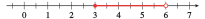
\includegraphics[width=1\linewidth]{images/fig-half-open-interval}
\caption{\label{fig-half-open-interval}}
\end{figure}
%
\item\hypertarget{li-124}{}\([−9,\infty)\). We always use round brackets next to the symbol \(\infty\) because \(\infty\) is not a specific number and is not included in the set. (See \hyperref[fig-half-closed-infinite-interval]{Figure~\ref{fig-half-closed-infinite-interval}}.) \leavevmode%
\begin{figure}
\centering
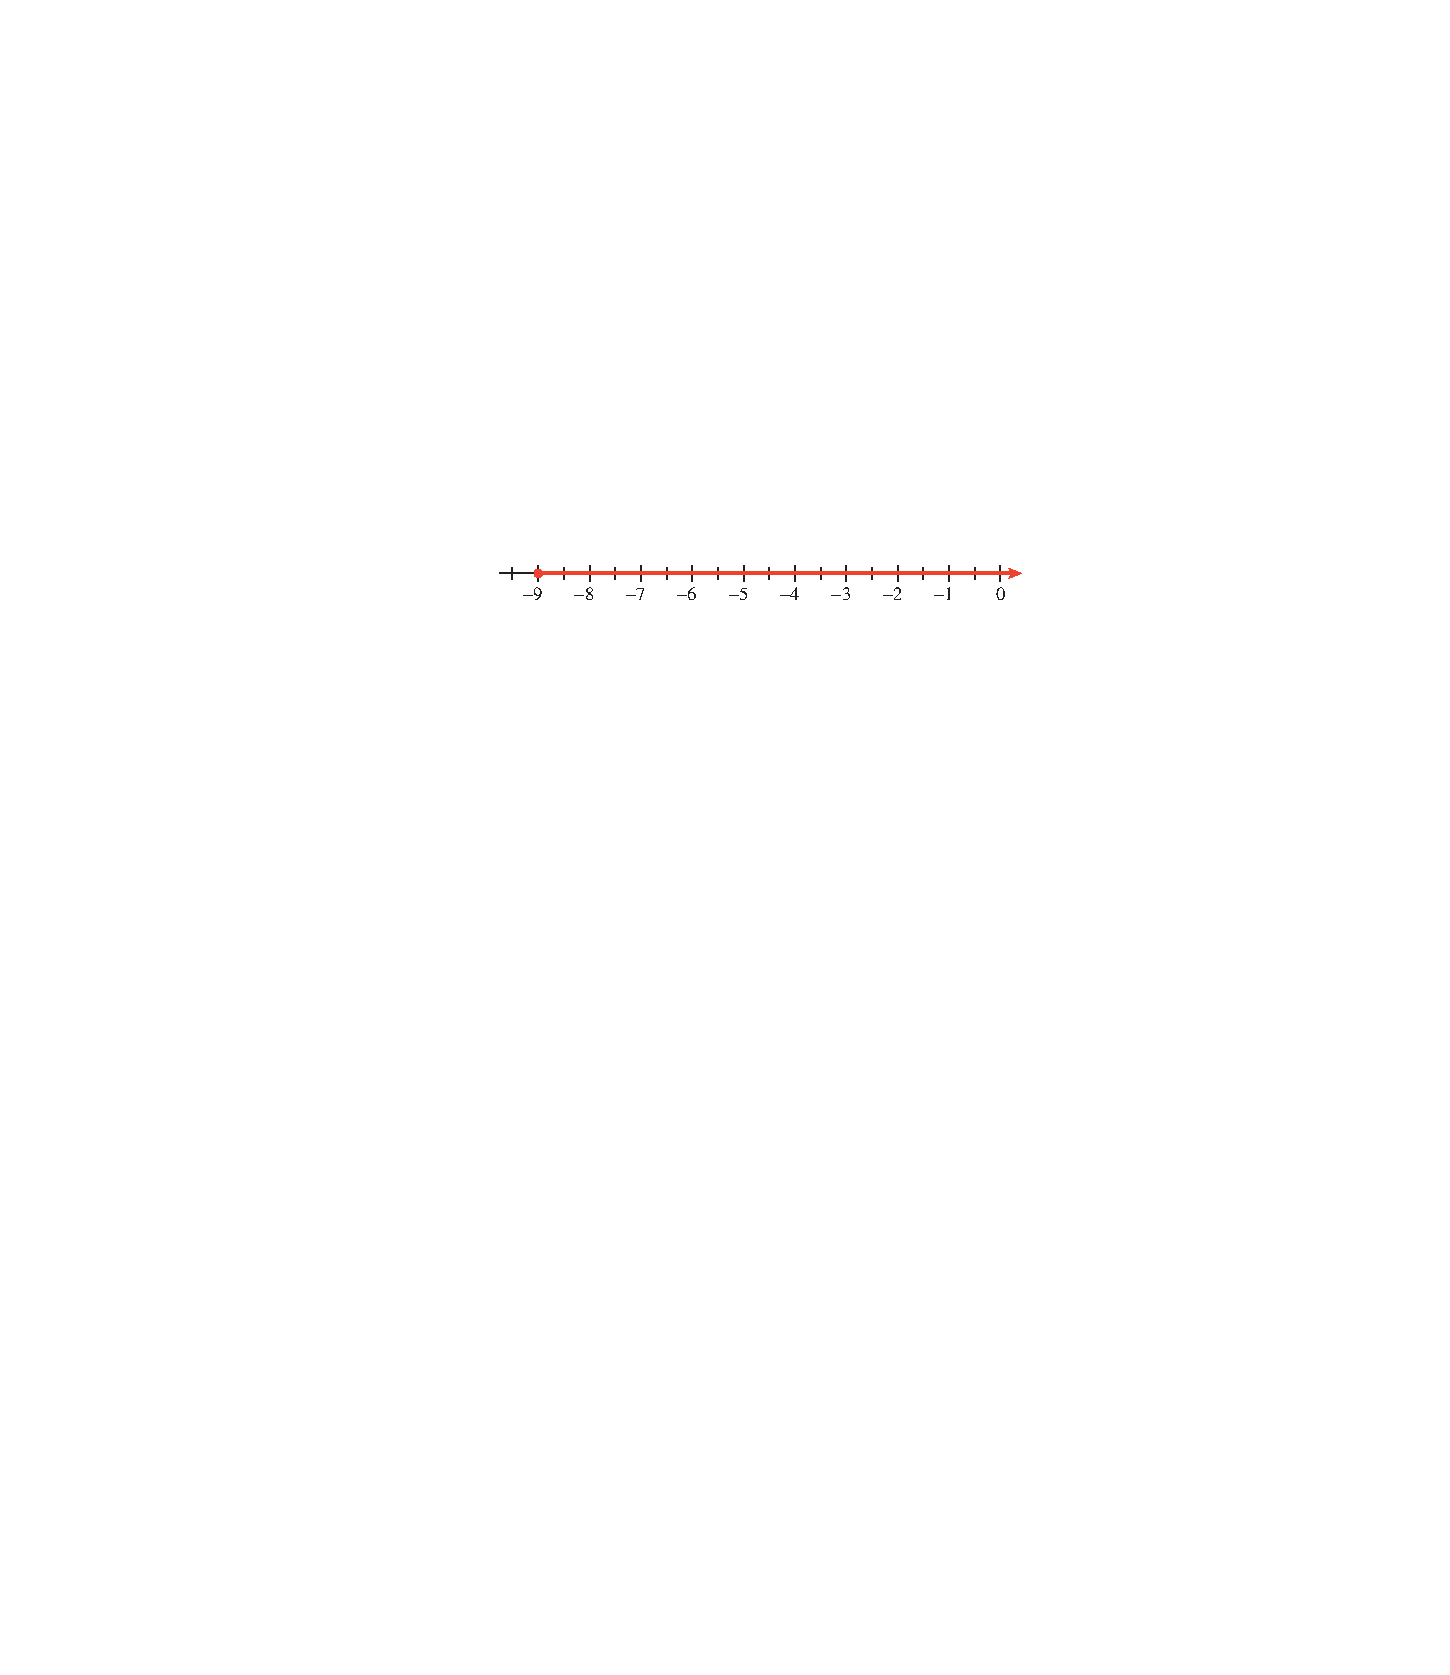
\includegraphics[width=1\linewidth]{images/fig-half-closed-infinite-interval}
\caption{\label{fig-half-closed-infinite-interval}}
\end{figure}
%
\item\hypertarget{li-125}{}\((−\infty, 1] \cup (4, \infty)\). The word \emph{or} describes the union of two sets. (See \hyperref[fig-disjoint-infinite-intervals]{Figure~\ref{fig-disjoint-infinite-intervals}}.) \leavevmode%
\begin{figure}
\centering
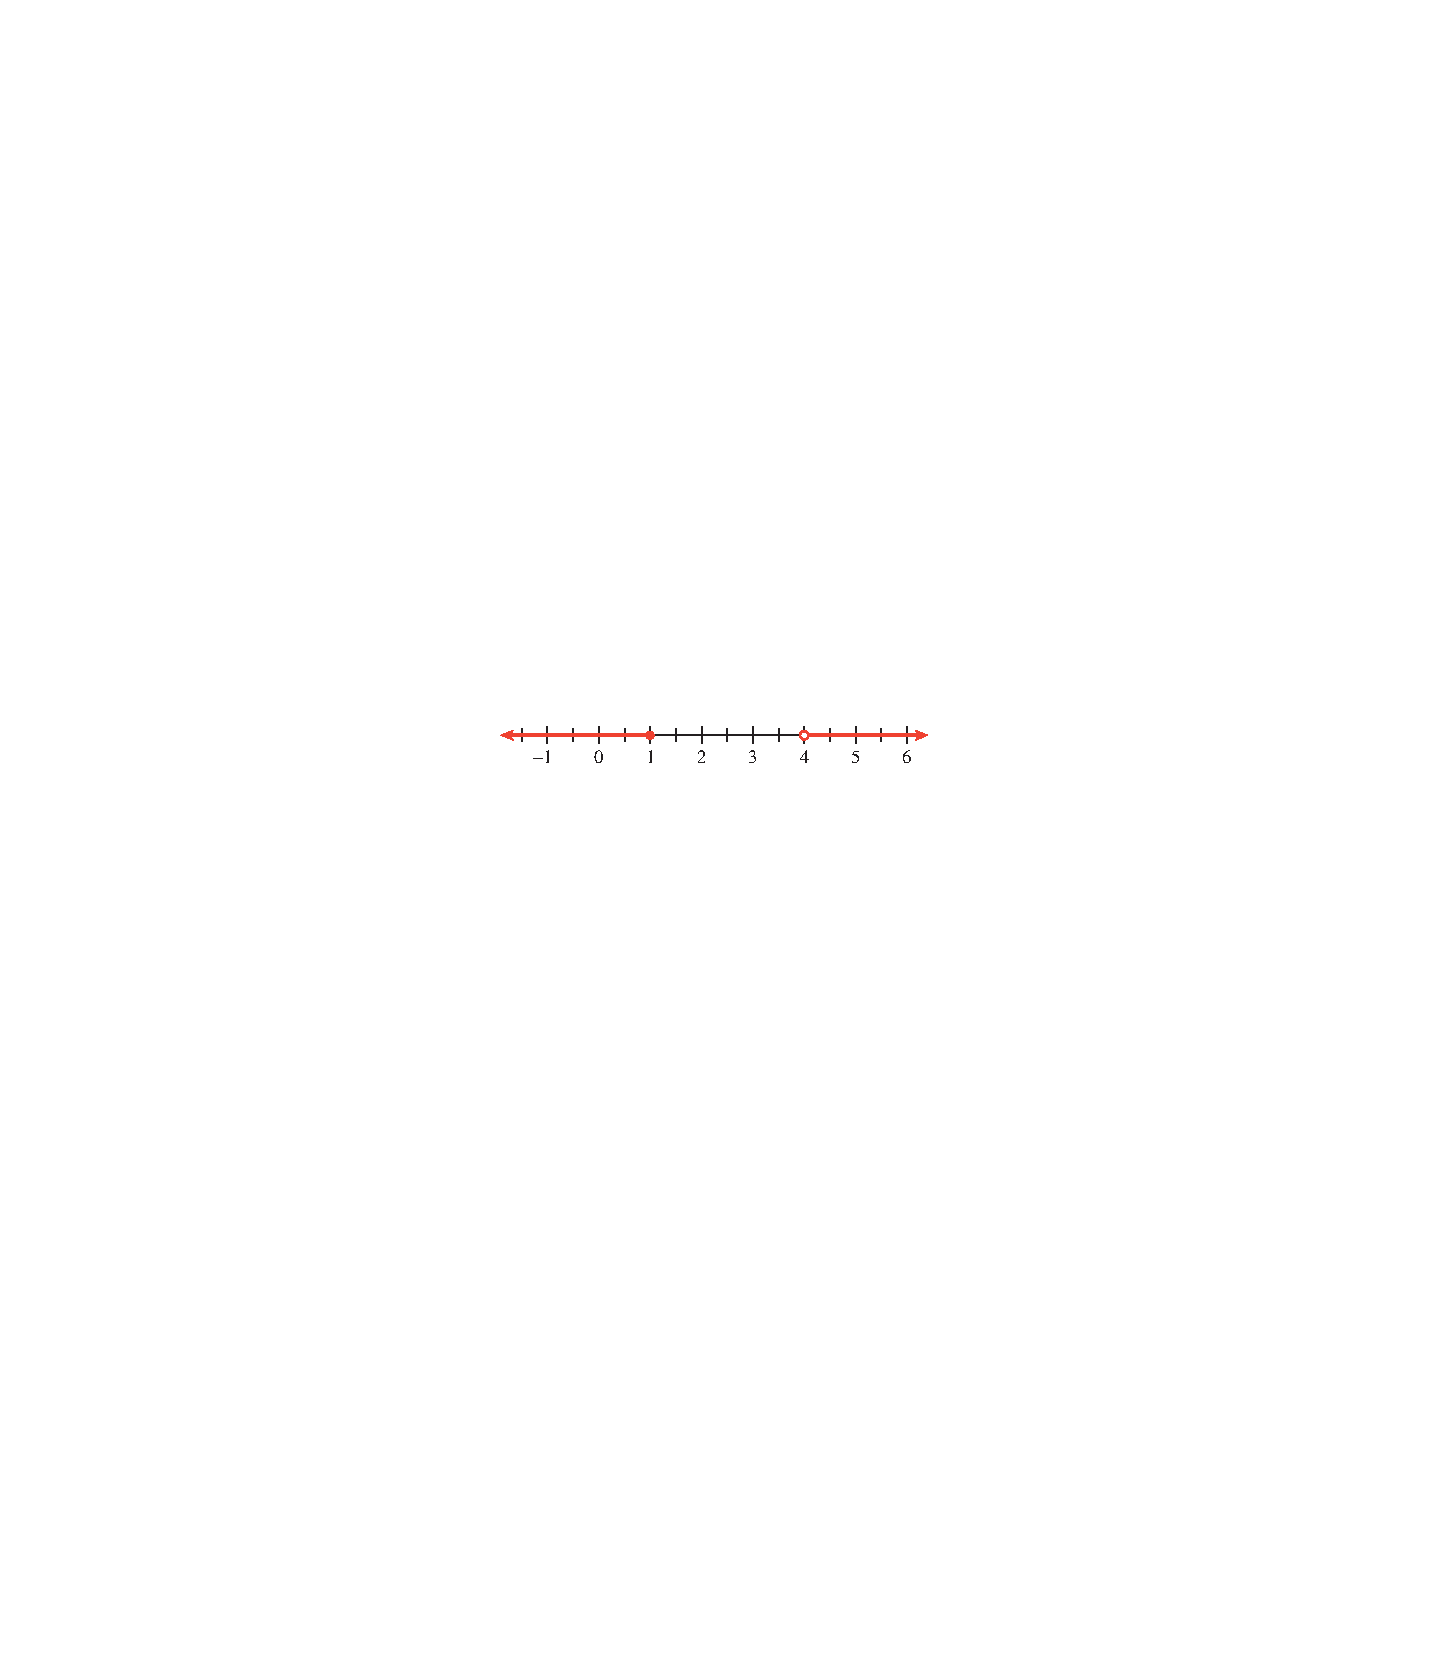
\includegraphics[width=1\linewidth]{images/fig-disjoint-infinite-intervals}
\caption{\label{fig-disjoint-infinite-intervals}}
\end{figure}
%
\item\hypertarget{li-126}{}\((−8,−5] \cup [−1, 3)\). (See \hyperref[fig-disjoint-finite-intervals]{Figure~\ref{fig-disjoint-finite-intervals}}.) \leavevmode%
\begin{figure}
\centering
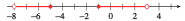
\includegraphics[width=1\linewidth]{images/fig-disjoint-finite-intervals}
\caption{\label{fig-disjoint-finite-intervals}}
\end{figure}
%
\end{enumerate}
%
\end{example}
\typeout{************************************************}
\typeout{Section A.3 Algebraic Expressions and Problem Solving}
\typeout{************************************************}
\section[{Algebraic Expressions and Problem Solving}]{Algebraic Expressions and Problem Solving}\label{appendix-Algebraic-Expressions-and-Problem-Solving}
You are familiar with the use of letters, or \terminology{variables}, to stand for unknown numbers in equations or formulas. Variables are also used to represent numerical quantities that change over time or in different situations. For example, \(p\) might stand for the atmospheric pressure at different heights above the Earth's surface. Or \(N\) might represent the number of people infected with cholera \(t\) days after the start of an epidemic.%
\par
An \terminology{algebraic expression} is any meaningful combination of numbers, variables, and symbols of operation. Algebraic expressions are used to express relationships between variable quantities.%
\begin{example}[]\label{example-Loren}
Loren makes \(\$6\) an hour working at the campus bookstore. \leavevmode%
\begin{enumerate}[label=*\alph**]
\item\hypertarget{li-127}{}Choose a variable for the number of hours Loren works per week.%
\item\hypertarget{li-128}{}Write an algebraic expression for the amount of Loren's weekly earnings.%
\end{enumerate}
%
\par\medskip\noindent%
\textbf{Solution.}\quad \leavevmode%
\begin{enumerate}[label=*\alph**]
\item\hypertarget{li-129}{}Let \(h\) stand for the number of hours Loren works per week.%
\item\hypertarget{li-130}{}The amount Loren earns is given by%
\begin{equation*}
6\times (\text{number of hours Loren worked})
\end{equation*}
or \(6\cdot h\). Loren's weekly earnings can be expressed as \(6h\).%
\end{enumerate}
%
\end{example}
\par
The algebraic expression \(6h\) represents the amount of money Loren earns \emph{in terms of} the number of hours she works. If we substitute a specific value for the variable in an expression, we find a numerical value for the expression. This is called \terminology{evaluating} the expression.%
\begin{example}[]\label{example-19}
If Loren from \hyperref[example-Loren]{Example~\ref{example-Loren}} works for \(16\) hours in the bookstore this week, how much will she earn?%
\par\medskip\noindent%
\textbf{Solution.}\quad Evaluate the expression \(6h\) for \(h=\alert{16}\).%
\begin{equation*}
6h = 6(\alert{16}) = 96
\end{equation*}
Loren will make \(\$96\).%
\end{example}
\begin{example}[]\label{example-April}
April sells environmentally friendly cleaning products. Her income consists of \(\$200\) per week plus a commission of \(9\%\) of her sales. \leavevmode%
\begin{enumerate}[label=*\alph**]
\item\hypertarget{li-131}{}Choose variables to represent the unknown quantities and write an algebraic expression for April's weekly income in terms of her sales.%
\item\hypertarget{li-132}{}Find April's income for a week in which she sells \(\$350\) worth of cleaning products.%
\end{enumerate}
%
\par\medskip\noindent%
\textbf{Solution.}\quad \leavevmode%
\begin{enumerate}[label=*\alph**]
\item\hypertarget{li-133}{}Let \(I\) represent April's total income for the week, and let \(S\) represent the total amount of her sales. We translate the information from the problem into mathematical language as follows:%
\begin{gather*}
\text{Her income consists of }\$200 . . .\text{ plus }. . . 9\% \text{ of her sales} 
\\
I \hphantom{consists of}= \hphantom{of}200 \hphantom{plus+}+ \hphantom{....}0.09 \hphantom{of her}S
\end{gather*}
Thus, \(I = 200 + 0.09S\).%
\item\hypertarget{li-134}{}We want to evaluate our expression from part (a) with \(S = 350\). We substitute \(\alert{350}\) for \(S\) to find%
\begin{equation*}
I = 200 + 0.09(\alert{350})
\end{equation*}
Following the order of operations, we perform the multiplication before the addition. Thus, we begin by computing \(0.09(350)\).%
\begin{align*}
I \amp = 200 + 0.09(350)\amp\amp\text{Multiply }0.09 (350) \text{ first.}
\\
\amp = 200 + 31.5\\
\amp = 231.50
\end{align*}
April's income for the week is \(\$231.50\).%
\end{enumerate}
%
\end{example}
\begin{remark}[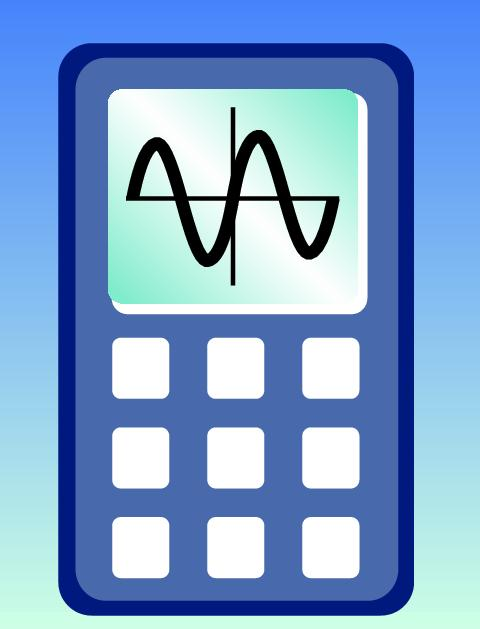
\includegraphics[width=0.08\linewidth]{images/icon-GC.jpg}
Calculator Tip]\label{remark-2}
On a scientific or a graphing calculator, we can enter the expression from \hyperref[example-April]{Example~\ref{example-April}} just as it is written:%
\begin{equation*}
200 + 0.09 ~ \boxed{\times}~ 350 ~\boxed{\text{ENTER}}
\end{equation*}
The calculator will perform the operations in the correct order—multiplication first.%
\end{remark}
\begin{example}[]\label{example-parcel}
Economy Parcel Service charges \(\$2.80\) per pound to deliver a package from Pasadena to Cedar Rapids. Andrew wants to mail a painting that weighs \(8.3\) pounds, plus whatever packing material he uses. \leavevmode%
\begin{enumerate}[label=*\alph**]
\item\hypertarget{li-135}{}Choose variables to represent the unknown quantities and write an expression for the cost of shipping Andrew's painting.%
\item\hypertarget{li-136}{}Find the shipping cost if Andrew uses \(2.9\) pounds of packing material.%
\end{enumerate}
%
\par\medskip\noindent%
\textbf{Solution.}\quad \leavevmode%
\begin{enumerate}[label=*\alph**]
\item\hypertarget{li-137}{}Let \(C\) stand for the shipping cost and let \(w\) stand for the weight of the packing material. Andrew must find the total weight of his package first, then multiply by the shipping charge. The total weight of the package is \(8.3 + w\) pounds. We use parentheses around this expression to show that it should be computed first, and the sum should be multiplied by the shipping charge of \(\$2.80\) per pound. Thus,%
\begin{equation*}
C = 2.80(8.3 + w)
\end{equation*}
%
\item\hypertarget{li-138}{}Evaluate the formula from part (a) with \(w = \alert{2.9}\).%
\begin{align*}
C \amp = 2.80(8.3 + \alert{2.9})\amp\amp\text{Add inside parentheses.}
\\
\amp = 2.80(11.2)\amp\amp\text{Multiply.}
\\
\amp = 31.36
\end{align*}
The cost of shipping the painting is \(\$31.36\).%
\end{enumerate}
%
\end{example}
\begin{remark}[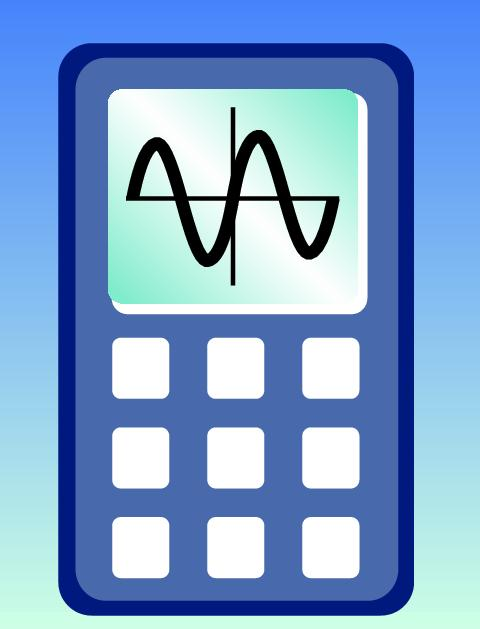
\includegraphics[width=0.08\linewidth]{images/icon-GC.jpg}
Calculator Tip]\label{remark-3}
On a calculator, we enter the expression for \(C\) in the order it appears, including the parentheses. (Experiment to see whether your calculator requires you to enter the \lstinline?×? symbol after 2.80.) The keying sequence%
\begin{equation*}
2.80 \times ( 8.3 + 2.9 ) \boxed{\text{ENTER}}
\end{equation*}
gives the correct result, \(31.36\).%
\end{remark}
\begin{warning}[]\label{warning-3}
If we omit the parentheses, the calculator will perform the multiplication before the addition. Thus, the keying sequence%
\begin{equation*}
2.80 \times 8.3 + 2.9
\end{equation*}
gives an incorrect result for \hyperref[example-parcel]{Example~\ref{example-parcel}}. (The sequence%
\begin{equation*}
8.3 + 2.9 \times 2.80
\end{equation*}
does not work either!)%
\end{warning}
\typeout{************************************************}
\typeout{Subsection A.3.1 Problem Solving}
\typeout{************************************************}
\subsection[{Problem Solving}]{Problem Solving}\label{subsection-13}
Problem solving often involves translating a real-life problem into a computer programming language, or, in our case, into algebraic expressions. We can then use algebra to solve the mathematical problem and interpret the solution in the context of the original problem. Here are some guidelines for problem solving with algebraic equations.%
\begin{assemblage}{Guidelines for Problem Solving}\label{assemblage-9}
\leavevmode%
\begin{description}
\item[{Step 1:}]\hypertarget{li-139}{}Identify the unknown quantity and assign a variable to represent it.%
\item[{Step 2:}]\hypertarget{li-140}{}Find some quantity that can be expressed in two different ways and write an equation.%
\item[{Step 3:}]\hypertarget{li-141}{}Solve the equation.%
\item[{Step 4:}]\hypertarget{li-142}{}Interpret your solution to answer the question in the problem.%
\end{description}
%
\end{assemblage}
\par
In step 1, begin by writing an English phrase to describe the quantity you are looking for. Be as specific as possible—if you are going to write an equation about this quantity, you must understand its properties! Remember that your variable must represent a numerical quantity. For example, \(x\) can represent the \emph{speed} of a train, but not just “the train.”%
\par
Writing an equation is the hardest part of the problem. Note that the quantity mentioned in step 2 will probably \emph{not} be the same unknown quantity you are looking for, but the algebraic expressions you write \emph{will} involve your variable. For example, if your variable represents the \emph{speed} of a train, your equation might be about the \emph{distance} the train traveled.%
\typeout{************************************************}
\typeout{Subsection A.3.2 Supply and Demand}
\typeout{************************************************}
\subsection[{Supply and Demand}]{Supply and Demand}\label{subsection-14}
The law of supply and demand is fundamental in economics. If you increase the price of a product, the supply increases because its manufacturers are willing to provide more of the product, but the demand decreases because consumers are not willing to buy as much at a higher price. The price at which the demand for a product equals the supply is called the \terminology{equilibrium price}.%
\begin{example}[]\label{example-22}
The Coffee Connection finds that when it charges \(p\) dollars for a pound of coffee, it can sell \(800 − 60p\) pounds per month. On the other hand, at a price of \(p\) dollars a pound, International Food and Beverage will supply the Connection with \(175 + 40p\) pounds of coffee per month. What price should the Coffee Connection charge for a pound of coffee so that its monthly inventory will sell out?%
\par\medskip\noindent%
\textbf{Solution.}\quad \leavevmode%
\begin{description}
\item[{Step 1:}]\hypertarget{li-143}{}We are looking for the equilibrium price, \(p\).%
\item[{Step 2:}]\hypertarget{li-144}{}The Coffee Connection would like the demand for its coffee to equal its supply. We equate the expressions for supply and for demand to obtain the equation%
\begin{equation*}
800 − 60p = 175 + 40p
\end{equation*}
%
\item[{Step 3:}]\hypertarget{li-145}{}Solve the equation. To get all terms containing the variable, \(p\), on one side of the equation, we add \(60p\) to both sides and subtract \(175\) from both sides to obtain%
\begin{align*}
800 − 60p + \alert{60p − 175} \amp= 175 + 40p + \alert{60p − 175}
\\
625 \amp = 100p \amp\amp\text{Divide both sides by }100.
\\
6.25 \amp = p
\end{align*}
%
\item[{Step 4:}]\hypertarget{li-146}{}The Coffee Connection should charge \(\$6.25\) per pound for its coffee.%
\end{description}
%
\end{example}
\typeout{************************************************}
\typeout{Subsection A.3.3 Percent Problems}
\typeout{************************************************}
\subsection[{Percent Problems}]{Percent Problems}\label{subsection-15}
Recall the basic formula for computing percents.%
\begin{assemblage}{Percent Formula}\label{assemblage-10}
%
\begin{equation*}
P = rW
\end{equation*}
the \terminology{P}art (or percent) = the percentage \terminology{r}ate \(\times\) the \terminology{W}hole Amount%
\end{assemblage}
\par
A \terminology{percent increase} or \terminology{percent decrease} is calculated as a fraction of the \emph{original} amount. For example, suppose you make \(\$16.00\) an hour now, but next month you are expecting a \(5\%\) raise. Your new salary should be%
\begin{equation*}
\stackrel{\text{Original salary}}{\$16.00} + \stackrel{\text{Increase}}{0.05(\$16.00)} = \stackrel{\text{New Salary}}{\$16.80}
\end{equation*}
%
\begin{example}[]\label{example-percent-increase}
The price of housing in urban areas increased \(4\%\) over the past year. If a certain house costs \(\$100,000\) today, what was its price last year?%
\par\medskip\noindent%
\textbf{Solution.}\quad \leavevmode%
\begin{description}
\item[{Step 1:}]\hypertarget{li-147}{}Let \(c\) represent the cost of the house last year.%
\item[{Step 2:}]\hypertarget{li-148}{}Express the current price of the house in two different ways. During the past year, the price of the house increased by \(4\%\), or \(0.04c\). Its current price is thus%
\begin{equation*}
\stackrel{\text{Original cost}}{(1)c} + \stackrel{\text{Price increase}}{0.04c} = c(1 + 0.04) = 1.04c
\end{equation*}
This expression is equal to the value given for current price of the house:%
\begin{equation*}
1.04c = 100,000
\end{equation*}
%
\item[{Step 3:}]\hypertarget{li-149}{}To solve this equation, we divide both sides by \(1.04\) to find%
\begin{equation*}
c = \frac{100,000}{1.04}= 96,153.846
\end{equation*}
%
\item[{Step 4:}]\hypertarget{li-150}{}To the nearest cent, the cost of the house last year was \(\$96,153.85\).%
\end{description}
%
\end{example}
\begin{warning}[]\label{warning-4}
In \hyperref[example-percent-increase]{Example~\ref{example-percent-increase}}, it would be incorrect to calculate last year's price by subtracting \(4\%\) of \(\$100,000\) from \(\$100,000\) to get \(\$96,000\). (Do you see why?)%
\end{warning}
\typeout{************************************************}
\typeout{Subsection A.3.4 Weighted Averages}
\typeout{************************************************}
\subsection[{Weighted Averages}]{Weighted Averages}\label{subsection-16}
We find the \terminology{average}, or \terminology{mean}, of a set of values by adding up the values and dividing the sum by the number of values. Thus, the average, \(\overline{x}\), of the numbers \(x_1, x_2, \ldots , x_n\) is given by%
\begin{equation*}
\overline{x} = \frac{x_1 + x_2 + ·· ·+x_n}{n}
\end{equation*}
In a \terminology{weighted average}, the numbers being averaged occur with different frequencies or are weighted differently in their contribution to the average value. For instance, suppose a biology class of 12 students takes a 10-point quiz. Of the 12 students, 2 receive 10s, three receive 9s, 5 receive 8s, and 2 receive scores of 6. The average score earned on the quiz is then%
\begin{equation*}
\overline{x} = \frac{\alert{2}(10) + \alert{3}(9) + \alert{5}(8) + \alert{2}(6)}{12}=8.25
\end{equation*}
The numbers in color are called the weights—in this example they represent the number of times each score was counted. Note that \(n\), the total number of scores, is equal to the sum of the weights:%
\begin{equation*}
12 = 2 + 3 + 5 + 2
\end{equation*}
%
\begin{example}[]\label{example-weighted-average}
Kwan's grade in his accounting class will be computed as follows: Tests count for \(50\%\) of the grade, homework counts for \(20\%\), and the final exam counts for \(30\%\). If Kwan has an average of \(84\) on tests and \(92\) on homework, what score does he need on the final exam to earn a grade of \(90\)?%
\par\medskip\noindent%
\textbf{Solution.}\quad \leavevmode%
\begin{description}
\item[{Step 1:}]\hypertarget{li-151}{}Let \(x\) represent the final exam score Kwan needs.%
\item[{Step 2:}]\hypertarget{li-152}{}Kwan's grade is the weighted average of his test, homework, and final exam scores.%
\begin{equation*}
\frac{\alert{0.50}(84) + \alert{0.20}(92) + \alert{0.30}x}{1.00}=90
\end{equation*}
(The sum of the weights is 1.00, or 100% of Kwan’s grade.) Multiply both sides of the equation by \(1.00\) to get%
\begin{equation*}
0.50(84) + 0.20(92) + 0.30x = 1.00(90)
\end{equation*}
%
\item[{Step 3:}]\hypertarget{li-153}{}Solve the equation. Simplify the left side first.%
\begin{align*}
60.4 + 0.30x \amp = 90\amp\amp\text{Subtract 60.4 from both sides.}
\\
0.30x \amp = 29.6\amp\amp\text{Divide both sides by 0.30.}
\\
x \amp = 98.7
\end{align*}
%
\item[{Step 4:}]\hypertarget{li-154}{}Kwan needs a score of \(98.7\) on the final exam to earn a grade of \(90\).%
\end{description}
%
\end{example}
\par
In step 2 of \hyperref[example-weighted-average]{Example~\ref{example-weighted-average}}, we rewrote the formula for a weighted average in a simpler form.%
\begin{assemblage}{Weighted Average}\label{assemblage-11}
The sum of the weighted values equals the sum of the weights times the average value. In symbols,%
\begin{equation*}
w_1x_1 + w_2x_2 + \cdots + w_nx_n = Wx
\end{equation*}
where \(W\) is the sum of the weights.%
\end{assemblage}
\par
This form is particularly useful for solving problems involving mixtures.%
\begin{example}[]\label{example-25}
The vet advised Delbert to feed his dog Rollo with kibble that is no more than \(8\%\) fat. Rollo likes JuicyBits, which are \(15\%\) fat. LeanMeal is more expensive, but it is only \(5\%\) fat. How much LeanMeal should Delbert mix with \(50\) pounds of JuicyBits to make amixture that is \(8\%\) fat?%
\par\medskip\noindent%
\textbf{Solution.}\quad \leavevmode%
\begin{description}
\item[{Step 1:}]\hypertarget{li-155}{}Let \(p\) represent the number of pounds of LeanMeal needed.%
\item[{Step 2:}]\hypertarget{li-156}{}In this problem, we want the weighted average of the fat contents in the two kibbles to be \(8\%\). The weights are the number of pounds of each kibble we use. It is often useful to summarize the given information in a table. \begin{tabular}{AlA}\hrulethin
\(\)&\(\%\) fat&Total pounds&Pounds of fat\tabularnewline\hrulethin
Juicy Bits&\(15\%\)&\(50\)&0.15(50)\tabularnewline\hrulethin
LeanMeal&\(5\%\)&\(p\)&0.05p\tabularnewline\hrulethin
Mixture&\(8\%\)&\(50+p\)&0.08(50+p)\tabularnewline\hrulethin
\end{tabular}
 The amount of fat in the mixture must come from adding the amounts of fat in the two ingredients. This gives us an equation,%
\begin{equation*}
0.15(50) + 0.05p = 0.08(50 + p)
\end{equation*}
This equation is an example of the formula for weighted averages.%
\item[{Step 3:}]\hypertarget{li-157}{}Simplify each side of the equation, then solve.%
\begin{align*}
7.5 + 0.05p \amp = 4 + 0.08p
\\
3.5 \amp = 0.03p
\\
p \amp = 116.\overline{6}
\end{align*}
%
\item[{Step 4:}]\hypertarget{li-158}{}Delbert should mix \(116\frac{2}{3}\) pounds of LeanMeal with \(50\) pounds of JuicyBits to make a mixture that is \(8\%\) fat.%
\end{description}
%
\end{example}
\typeout{************************************************}
\typeout{Section A.4 Graphs and Equations}
\typeout{************************************************}
\section[{Graphs and Equations}]{Graphs and Equations}\label{appendix-Graphs-and-Equations}
Graphs are useful tools for studying mathematical relationships. A graph provides an overview of a quantity of data, and it helps us identify trends or unexpected occurrences. Interpreting the graph can help us answer questions about the data.%
\par
For example, here are some data showing the atmospheric pressure at different altitudes. Altitude is given in feet, and atmospheric pressure is given in inches of mercury. \leavevmode%
\begin{table}
\centering
\begin{tabular}{AlA}\hrulethin
Altitude (ft)&\(0\)&\(5000\)&\(10,000\)&\(20,000\)&\(30,000\)&\(40,000\)&\(50,000\)\tabularnewline\hrulethin
Pressure (in. Hg)&\(29.7\)&\(24.8\)&\(20.5\)&\(14.6\)&\(10.6\)&\(8.5\)&\(7.3\)\tabularnewline\hrulethin
\end{tabular}
\end{table}
%
\par
We observe a generally decreasing trend in pressure as the altitude increases, but it is difficult to say anything more precise about this relationship. A clearer picture emerges if we plot the data. To do this, we use two perpendicular number lines called axes. We use the horizontal axis for the values of the first variable, altitude, and the vertical axis for the values of the second variable, pressure.%
\par
The entries in the table are called \terminology{ordered pairs}, in which the \terminology{first component} is the altitude and the \terminology{second component} is the atmospheric pressure measured at that altitude. For example, the first two entries can be represented by \((0, 29.7)\) and \((5000, 24.8)\). We plot the points whose \terminology{coordinates} are given by the ordered pairs, as shown in \hyperref[fig-pressure-vs-altitude]{Figure~\ref{fig-pressure-vs-altitude}}a. \leavevmode%
\begin{figure}
\centering
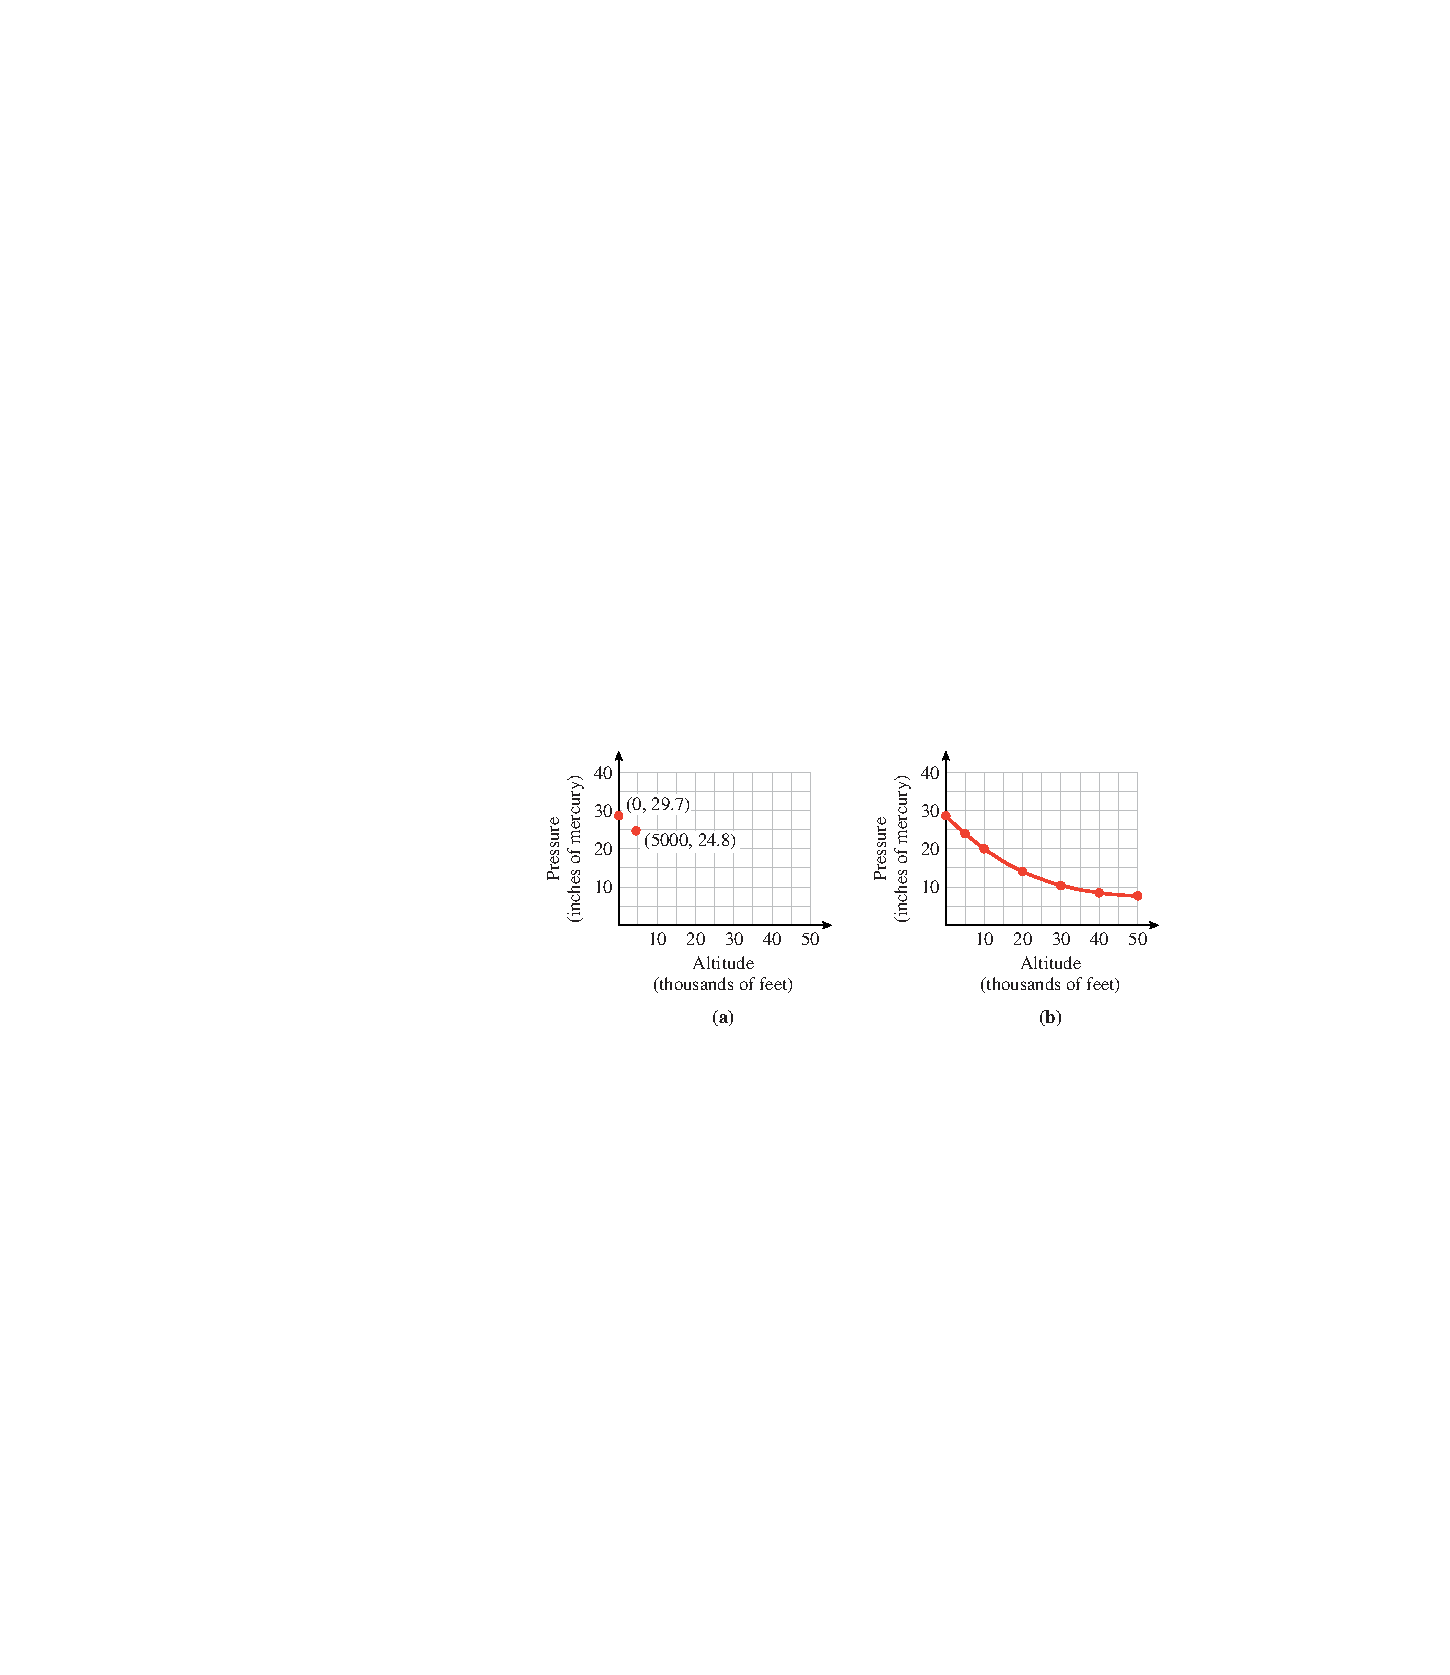
\includegraphics[width=1\linewidth]{images/fig-pressure-vs-altitude}
\caption{\label{fig-pressure-vs-altitude}}
\end{figure}
%
\par
We can connect the data points with a smooth curve as shown in \hyperref[fig-pressure-vs-altitude]{Figure~\ref{fig-pressure-vs-altitude}}b. In doing this, we are assuming that one variable changes smoothly with respect to the other, and in fact this is true for many physical situations. Thus, a smooth curve will thus serve as a good model.%
\typeout{************************************************}
\typeout{Subsection A.4.1 Reading a Graph}
\typeout{************************************************}
\subsection[{Reading a Graph}]{Reading a Graph}\label{subsection-17}
Once we have constructed a graph, we can use it to estimate values of the variables between the known data points.%
\begin{example}[]\label{example-pressure-vs-altitude}
From the graph in \hyperref[fig-pressure-vs-altitude]{Figure~\ref{fig-pressure-vs-altitude}}b, estimate the following: \leavevmode%
\begin{enumerate}[label=*\alph**]
\item\hypertarget{li-159}{}The atmospheric pressure measured at an altitude of \(15,000\) feet%
\item\hypertarget{li-160}{}The altitude at which the pressure is \(12\) inches of mercury%
\end{enumerate}
%
\par\medskip\noindent%
\textbf{Solution.}\quad \leavevmode%
\begin{enumerate}[label=*\alph**]
\item\hypertarget{li-161}{}The point with first coordinate \(15,000\) on the graph in \hyperref[fig-pressure-vs-altitude2]{Figure~\ref{fig-pressure-vs-altitude2}} has second coordinate approximately \(17.4\). We estimate the pressure at \(15,000\) feet to be \(17.4\) inches of mercury. \leavevmode%
\begin{figure}
\centering
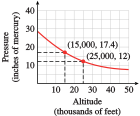
\includegraphics[width=0.6\linewidth]{images/fig-pressure-vs-altitude2}
\caption{\label{fig-pressure-vs-altitude2}}
\end{figure}
%
\item\hypertarget{li-162}{}The point on the graph with second coordinate \(12\) has first coordinate approximately \(25,000\), so an atmospheric pressure of \(12\) inches of mercury occurs at about \(25,000\) feet.%
\end{enumerate}
%
\end{example}
\par
We can also use the graph to obtain information about the relationship between altitude and pressure that would be difficult to see from the data alone.%
\begin{example}[]\label{example-27}
\leavevmode%
\begin{enumerate}[label=*\alph**]
\item\hypertarget{li-163}{}For what altitudes is the pressure less than \(18\) inches of mercury?%
\item\hypertarget{li-164}{}How much does the pressure decrease as the altitude increases from \(15,000\) feet to \(25,000\) feet?%
\item\hypertarget{li-165}{}For which \(10,000\)-foot increase in altitude does the pressure change most rapidly?%
\end{enumerate}
%
\par\medskip\noindent%
\textbf{Solution.}\quad \leavevmode%
\begin{enumerate}[label=*\alph**]
\item\hypertarget{li-166}{}From the graph in \hyperref[fig-pressure-vs-altitude]{Figure~\ref{fig-pressure-vs-altitude}}b, we see that the pressure has dropped to \(18\) inches of mercury at about \(14,000\) feet, and that it continues to decrease as the altitude increases. Therefore, the pressure is less than \(18\) inches of mercury for altitudes greater than \(14,000\) feet.%
\item\hypertarget{li-167}{}The pressure at \(15,000\) feet is approximately \(17.4\) inches of mercury, and at \(25,000\) feet it is \(12\) inches. This represents a decrease in pressure of \(17.4 − 12\), or \(5.4\), inches of mercury.%
\item\hypertarget{li-168}{}By studying the graph we see that the pressure decreases most rapidly at low altitudes, so we conclude that the greatest drop in pressure occurs between \(0\) and \(10,000\) feet.%
\end{enumerate}
%
\end{example}
\typeout{************************************************}
\typeout{Subsection A.4.2 Graphs of Equations}
\typeout{************************************************}
\subsection[{Graphs of Equations}]{Graphs of Equations}\label{subsection-18}
In \hyperref[example-pressure-vs-altitude]{Example~\ref{example-pressure-vs-altitude}}, we used a graph to illustrate data given in a table. Graphs can also help us analyze models given by equations. Let us first review some facts about solutions of equations in two variables.%
\par
An equation in two variables, such as y = 2x + 3, is said to be satisfied if the variables are replaced by a pair of numbers that make the statement true. The pair of numbers is called a \terminology{solution} of the equation and is usually written as an ordered pair \((x, y)\). (The first number in the pair is the value of \(x\) and the second number is the value of \(y\).)%
\par
To find a solution of a given equation, we can assign a number to one of the variables and then solve for the second variable.%
\begin{example}[]\label{example-28}
Find solutions to the equation \(y = 2x + 3\).%
\par\medskip\noindent%
\textbf{Solution.}\quad We choose some values for \(x\), say, \(-2\), \(0\), and \(1\). Substitute these \(x\)-values into the equation to find a corresponding \(y\)-value for each.%
\begin{align*}
\amp\text{When }x=−2,\amp\amp y = 2(\alert{−2}) + 3 =−1
\\
\amp\text{When }x=0,\amp\amp y = 2(\alert{0}) + 3 =3
\\
\amp\text{When }x=1,\amp\amp y = 2(\alert{1}) + 3 =5
\end{align*}
Thus, the ordered pairs \((−2, −1)\), \((0, 3)\), and \((1, 5)\) are three solutions of \(y = 2x + 3\). We can also substitute values for \(y\). For example, if we let \(y = \alert{10}\), we have%
\begin{equation*}
\alert{10} = 2x + 3
\end{equation*}
Solving this equation for \(x\), we find \(7 = 2x\), or \(x = 3.5\). This means that the ordered pair \((3.5, 10)\) is another solution of the equation \(y = 2x + 3\).%
\end{example}
\par
An equation in two variables may have infinitely many solutions, so we cannot list them all. However, we can display the solutions on a graph. For this we use a \terminology{Cartesian} (or \terminology{rectangular}) \terminology{coordinate system}, as shown in \hyperref[fig-coordinate-plane]{Figure~\ref{fig-coordinate-plane}}.%
% group protects changes to lengths, releases boxes (?)
{% begin: group for a single side-by-side
% set panel max height to practical minimum, created in preamble
\setlength{\panelmax}{0pt}
\newsavebox{\panelboxADimage}
\savebox{\panelboxADimage}{%
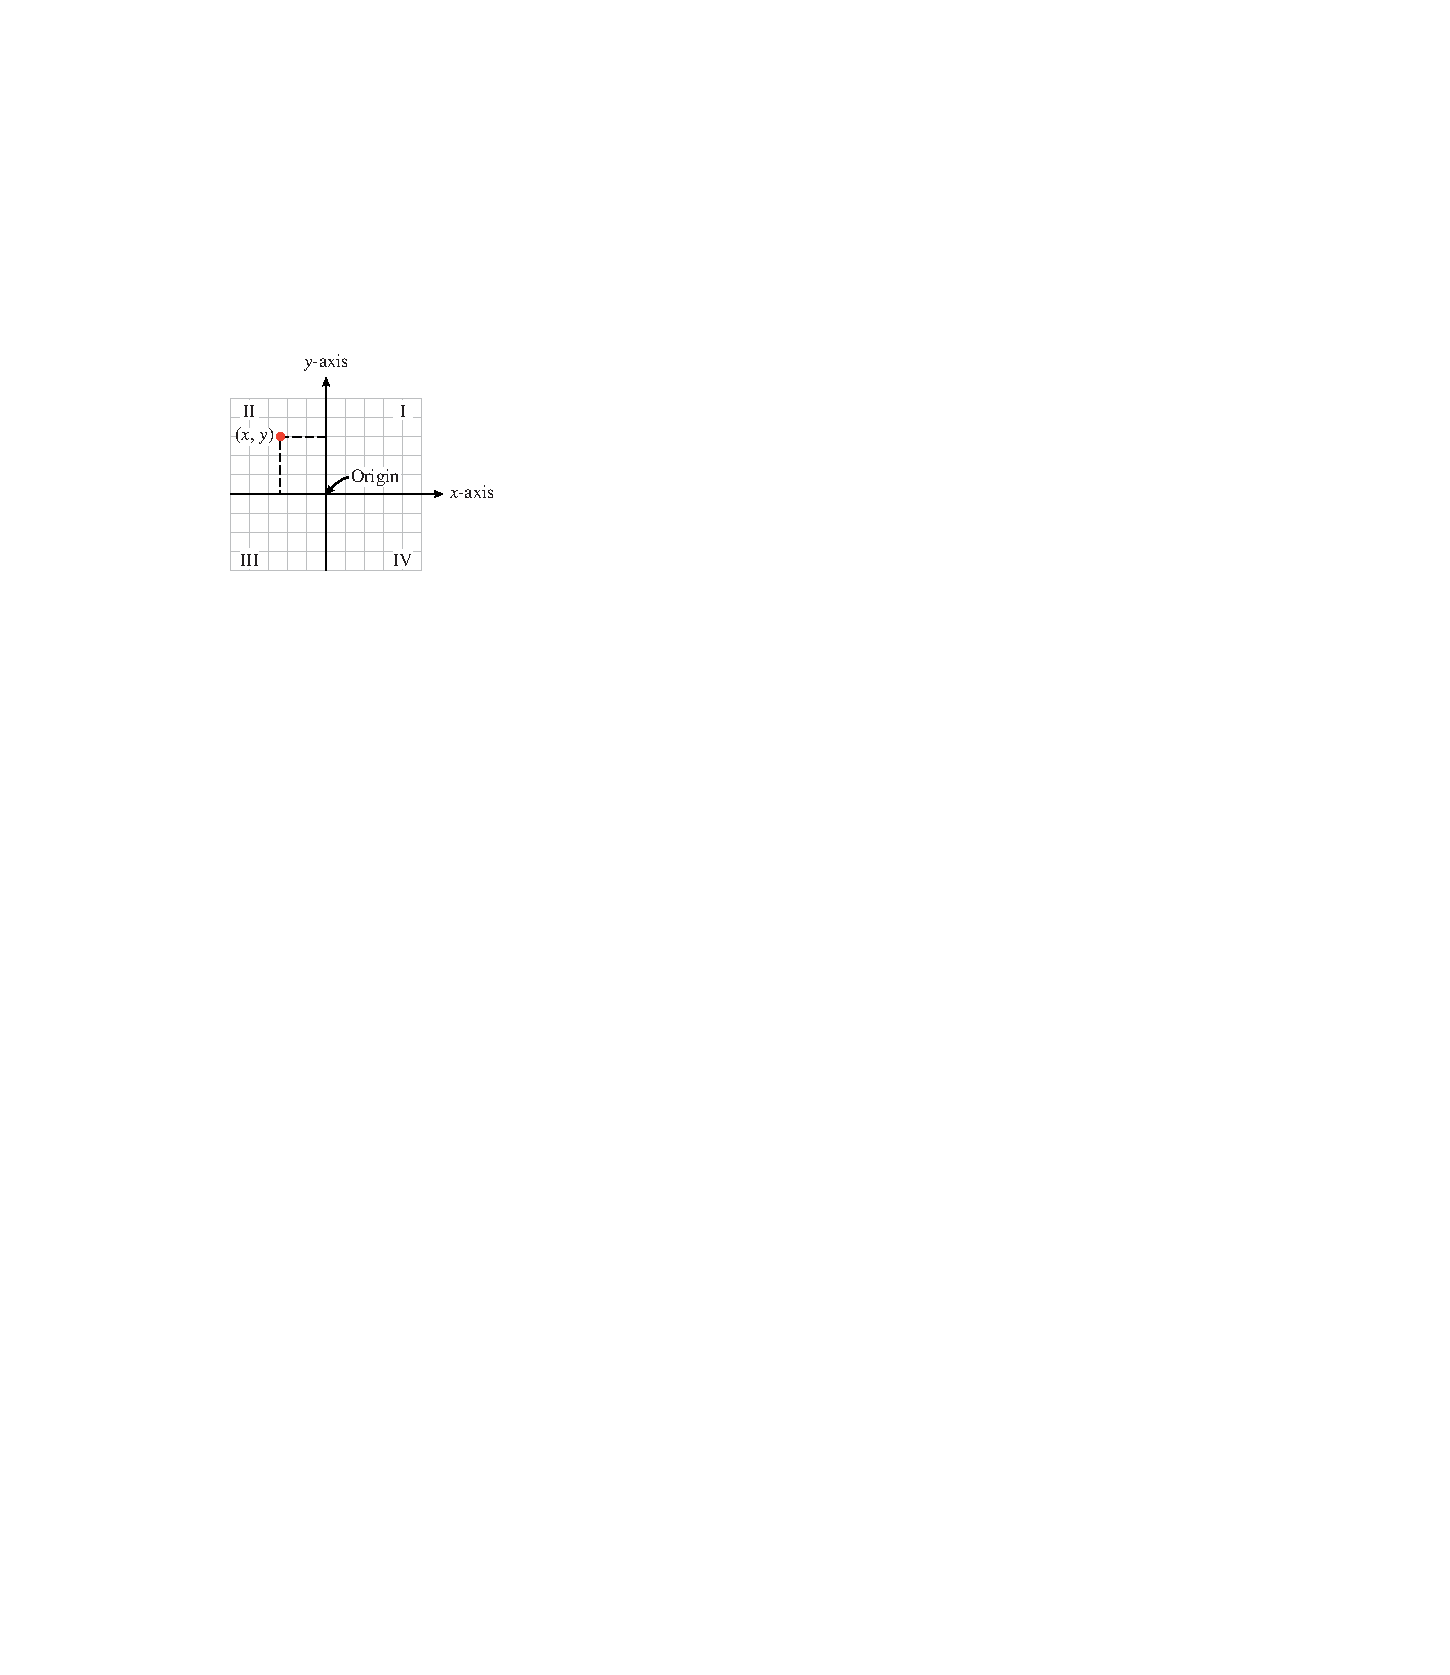
\includegraphics[width=0.45\linewidth]{images/fig-coordinate-plane}
}
\newlength{\phADimage}\setlength{\phADimage}{\ht\panelboxADimage+\dp\panelboxADimage}
\settototalheight{\phADimage}{\usebox{\panelboxADimage}}
\setlength{\panelmax}{\maxof{\panelmax}{\phADimage}}
\newsavebox{\panelboxAEimage}
\savebox{\panelboxAEimage}{%
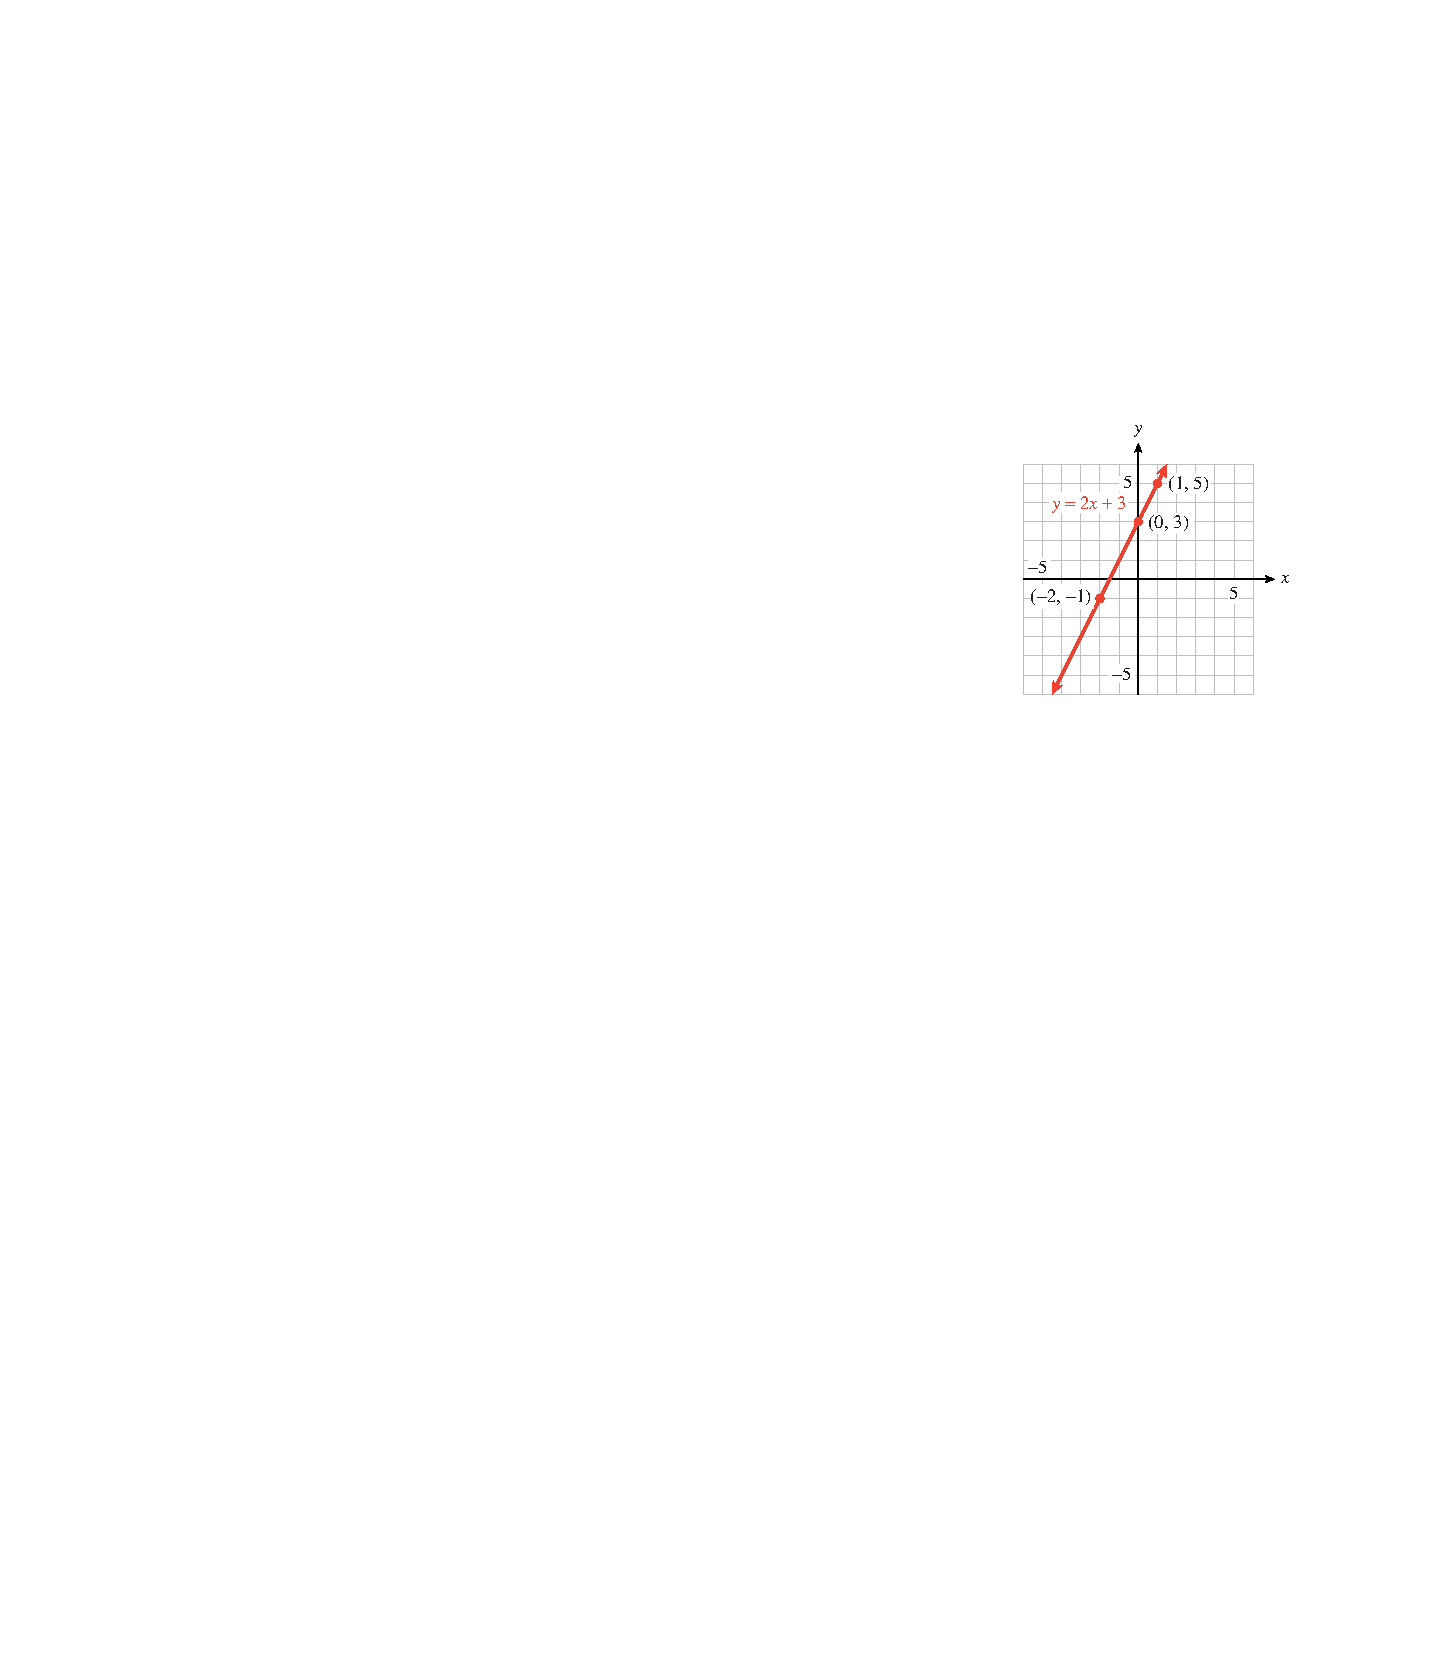
\includegraphics[width=0.45\linewidth]{images/fig-line}
}
\newlength{\phAEimage}\setlength{\phAEimage}{\ht\panelboxAEimage+\dp\panelboxAEimage}
\settototalheight{\phAEimage}{\usebox{\panelboxAEimage}}
\setlength{\panelmax}{\maxof{\panelmax}{\phAEimage}}
\leavevmode%
% begin: side-by-side as figure/tabular
% \tabcolsep change local to group
\setlength{\tabcolsep}{0.025\textwidth}
% @{} suppress \tabcolsep at extremes, so margins behave as intended
\begin{figure}
\hspace*{0.025\textwidth}%
\begin{tabular}{@{}*{2}{c}@{}}
\begin{minipage}[c][\panelmax][t]{0.45\textwidth}\usebox{\panelboxADimage}\end{minipage}&
\begin{minipage}[c][\panelmax][t]{0.45\textwidth}\usebox{\panelboxAEimage}\end{minipage}\tabularnewline
\parbox[t]{0.45\textwidth}{\captionof{figure}{\label{fig-coordinate-plane}}
}&
\parbox[t]{0.45\textwidth}{\captionof{figure}{\label{fig-line}}
}\end{tabular}
\end{figure}
% end: side-by-side as tabular/figure
}% end: group for a single side-by-side
\par
The \terminology{graph of an equation} is a picture of its solutions. A point is included in the graph if its coordinates satisfy the equation, and if the coordinates do not satisfy the equation, the point is not part of the graph. A graph of \(y = 2x + 3\) is shown in \hyperref[fig-line]{Figure~\ref{fig-line}}.%
\par
This graph does not display \emph{all} the solutions of the equation, but it shows important features such as the intercepts on the \(x\)- and \(y\)-axes. Because there is a solution corresponding to every real number \(x\), the graph extends infinitely in either direction, as indicated by the arrows.%
\begin{example}[]\label{example-29}
Use the graph of \(y = 0.5x^2 − 2\) in \hyperref[fig-parabola0]{Figure~\ref{fig-parabola0}} to decide whether the given ordered pairs are solutions of the equation. Verify your answers algebraically. \leavevmode%
\begin{enumerate}[label=*\alph**]
\item\hypertarget{li-169}{}\((−4, 6)\)%
\item\hypertarget{li-170}{}\((3, 0)\)%
\end{enumerate}
 \leavevmode%
\begin{figure}
\centering
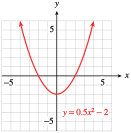
\includegraphics[width=0.45\linewidth]{images/fig-parabola0}
\caption{\label{fig-parabola0}}
\end{figure}
%
\par\medskip\noindent%
\textbf{Solution.}\quad \leavevmode%
\begin{enumerate}[label=*\alph**]
\item\hypertarget{li-171}{}Because the point \((−4, 6)\) does lie on the graph, the ordered pair \(x=−4, y = 6\) is a solution of \(y = 0.5x^2 − 2\). We can verify this by substituting \(\alert{-4}\) for \(x\) and \(\blert{6}\) for \(y\):%
\begin{align*}
0.5(\alert{-4})^2 − 2 \amp= 0.5(16) − 2\\
= 8 − 2 \amp = \blert{6}
\end{align*}
%
\item\hypertarget{li-172}{}Because the point \((3, 0)\) does not lie on the graph, the ordered pair \(x = 3, y = 0\) is not a solution of \(y = 0.5x^2 − 2\). We substitute \(\alert{3}\) for \(x\) and \(\blert{0}\) for \(y\) to verify this.%
\begin{align*}
0.5(\alert{3})^2 − 2 \amp= 0.5(9) − 2\\
= 4.5 − 2 \amp = 2.5 \ne \blert{0}
\end{align*}
%
\end{enumerate}
%
\end{example}
\typeout{************************************************}
\typeout{Section A.5 Linear Systems in Two Variables}
\typeout{************************************************}
\section[{Linear Systems in Two Variables}]{Linear Systems in Two Variables}\label{appendix-Linear-Systems-in-Two-Variables}
\index{linear system}A \(2\times 2\) \terminology{system} of equations is a set of \(2\) equations in the same \(2\) variables. A \terminology{solution} of a \(2\times 2\) system is an ordered pair that makes each equation in the system true. In this section, we review two algebraic methods for solving \(2\times 2\) linear systems: substitution and elimination.%
\typeout{************************************************}
\typeout{Subsection A.5.1 Solving Systems by Substitution}
\typeout{************************************************}
\subsection[{Solving Systems by Substitution}]{Solving Systems by Substitution}\label{subsection-19}
The basic strategy for the \terminology{substitution} method can be described as follows.%
\begin{assemblage}{Steps for Solving a \(\text{}\) System by Substitution}\label{assemblage-12}
\leavevmode%
\begin{enumerate}[label=*\arabic**]
\item\hypertarget{li-173}{}Solve one of the equations for one of the variables in terms of the other.%
\item\hypertarget{li-174}{}Substitute this expression into the second equation; doing so yields an equation in one variable.%
\item\hypertarget{li-175}{}Solve the new equation.%
\item\hypertarget{li-176}{}Use the result of step 1 to find the other variable.%
\end{enumerate}
%
\end{assemblage}
\begin{example}[]\label{example-30}
Staci stocks two kinds of sleeping bags in her sporting goods store, a standard model and a down-filled model for colder temperatures. From past experience, she estimates that she will sell twice as many of the standard variety as of the down filled. She has room to stock 60 sleeping bags at a time. How many of each variety should Staci order?%
\par\medskip\noindent%
\textbf{Solution.}\quad \leavevmode%
\begin{description}
\item[{Step 1:}]\hypertarget{li-177}{}%
\begin{align*}
\amp\text{Number of standard sleeping bags: }~x\\
\amp\text{Number of down-filled sleeping bags: }~y
\end{align*}
%
\item[{Step 2:}]\hypertarget{li-178}{}Write two equations about the variables. Staci needs twice as many standard model as down filled, so%
\begin{align*}
x \amp = 2y\amp\amp\hphantom{blankety}(1)
\end{align*}
Also, the total number of sleeping bags is 60, so%
\begin{align*}
x+y \amp = 60\amp\amp\hphantom{blank}(2)
\end{align*}
%
\item[{Step 3:}]\hypertarget{li-179}{}We will solve this system using substitution. Notice that Equation (1) is already solved for \(x\) in terms of \(y\): \(x = 2y\). Substitute \(\alert{2y}\) for \(x\) in Equation (2) to obtain%
\begin{align*}
\alert{2y} + y \amp = 60
\\
3y\amp = 60
\end{align*}
Solving for \(y\), we find \(y=\alert{20}\). Finally, substitute this value into Equation (1) to find%
\begin{equation*}
x = 2(\alert{20}) = 40
\end{equation*}
The solution to the system is \(x = 40, y = 20\).%
\item[{Step 4:}]\hypertarget{li-180}{}Staci should order \(40\) standard sleeping bags and \(20\) down-filled bags.%
\end{description}
%
\end{example}
\typeout{************************************************}
\typeout{Subsection A.5.2 Solving Systems by Elimination}
\typeout{************************************************}
\subsection[{Solving Systems by Elimination}]{Solving Systems by Elimination}\label{subsection-20}
The method of substitution is convenient if one of the variables in the system has a coefficient of \(1\) or \(-1\), because it is easy to solve for that variable. If none of the coefficients is \(1\) or \(-1s\), then a second method, called \terminology{elimination}, is usually more efficient.%
\par
The method of elimination is based on the following properties of linear equations.%
\begin{assemblage}{Properties of Linear Systems}\label{assemblage-13}
\leavevmode%
\begin{enumerate}[label=*\arabic**]
\item\hypertarget{li-181}{}Multiplying a linear equation by a (nonzero) constant does not change its solutions. That is, any solution of the equation%
\begin{equation*}
ax + by = c
\end{equation*}
is also a solution of the equation%
\begin{equation*}
kax + kby = kc
\end{equation*}
%
\item\hypertarget{li-182}{}Adding (or subtracting) two linear equations does not change their common solutions. That is, any solution of the system%
\begin{align*}
a_1x + b_1 y \amp = c_1\\
a_2x + b_2 y \amp = c_2
\end{align*}
is also a solution of the equation%
\begin{equation*}
(a_1 + a_2) x + (b_1 + b_2) y = c_1 + c_2
\end{equation*}
%
\end{enumerate}
%
\end{assemblage}
\begin{example}[]\label{example-linear-combinations}
Solve the system by the method of elimination.%
\begin{alignat*}{3}
2x\amp {}+{}\amp 3y\amp ={}\amp 8 \hphantom{blankblank}\amp(1)\\
3x\amp {}-{}\amp 4y\amp ={}\amp -5 \hphantom{blankblank}\amp(2)
\end{alignat*}
%
\par\medskip\noindent%
\textbf{Solution.}\quad We first decide which variable to eliminate, \(x\) or \(y\). We can choose whichever looks easiest. In this problem, we choose to eliminate \(x\). We next look for the smallest number that both coefficients, \(2\) and \(3\), divide into evenly. This number is \(6\). We want the coefficients of \(x\) to become \(6\) and \(-6\), so we will multiply Equation (1) by \(3\) and Equation (2) by \(-2\) to obtain%
\begin{alignat*}{3}
6x\amp {}+{}\amp 9y\amp ={}\amp 24 \hphantom{blankblank}\amp(1\text{a})\\
-6x\amp {}+{}\amp 8y\amp ={}\amp 10 \hphantom{blankblank}\amp(2\text{a})
\end{alignat*}
Now add the corresponding terms of (1a) and (2a). The \(x\)-terms are eliminated, yielding an equation in one variable.%
\begin{alignat*}{3}
6x\amp {}+{}\amp 9y\amp ={}\amp 24 \hphantom{blankblank}\amp(1\text{a})\\
-6x\amp {}+{}\amp 8y\amp ={}\amp 10 \hphantom{blankblank}\amp(2\text{a})\\
{}\amp {}{}\amp 17y\amp ={}\amp 34 \hphantom{blankblank}\amp(3)
\end{alignat*}
Solve this equation for \(y\) to find \(y=\alert{2}\). We can substitute this value of \(y\) into any of our equations involving both \(x\) and \(y\). If we choose Equation (1), then%
\begin{equation*}
2x + 3 (\alert{2}) = 8
\end{equation*}
and solving this equation yields \(x=1\). The ordered pair \((1, 2)\) is a solution to the system. You should verify that these values satisfy both original equations.%
\end{example}
\par
We summarize the strategy for solving a linear system by elimination.%
\begin{assemblage}{Steps for Solving a \(2\times 2\) Linear System by Elimination}\label{assemblage-14}
\leavevmode%
\begin{enumerate}[label=*\arabic**]
\item\hypertarget{li-183}{}Choose one of the variables to eliminate. Multiply each equation by a suitable factor so that the coefficients of that variable are opposites.%
\item\hypertarget{li-184}{}Add the two new equations termwise.%
\item\hypertarget{li-185}{}Solve the resulting equation for the remaining variable.%
\item\hypertarget{li-186}{}Substitute the value found in step 3 into either of the original equations and solve for the other variable.%
\end{enumerate}
%
\end{assemblage}
\par
In \hyperref[example-linear-combinations]{Example~\ref{example-linear-combinations}}, we added \(3\) times the first equation to \(-2\) times the second equation. The result from adding a constant multiple of one equation to a constant multiple of another equation is called a \terminology{linear combination} of the two equations. The method of elimination is also called the method of linear combinations\index{linear combinations}.%
\par
If either equation in a system has fractional coefficients, it is helpful to clear the fractions before applying the method of linear combinations.%
\begin{example}[]\label{example-32}
Solve the system by linear combinations.%
\begin{alignat*}{3}
\frac{2}{3}x\amp {}-{}\amp y\amp ={}\amp 2 \hphantom{blankblank}\amp(1)\\
x\amp {}+{}\amp \frac{1}{2}y\amp ={}\amp 7 \hphantom{blankblank}\amp(2)
\end{alignat*}
%
\par\medskip\noindent%
\textbf{Solution.}\quad Multiply each side of Equation (1) by \(3\) and each side of Equation (2) by \(2\) to clear the fractions:%
\begin{alignat*}{3}
2x\amp {}-{}\amp 3y\amp ={}\amp 6 \hphantom{blankblank}\amp(1\text{a})\\
2x\amp {}+{}\amp y\amp ={}\amp 14 \hphantom{blankblank}\amp(2\text{a})
\end{alignat*}
To eliminate the variable \(x\), multiply Equation (2a) by \(-1\) and add the result to Equation (1a) to get%
\begin{align*}
−4y \amp = −8 \amp\amp\text{Divide both sides by −4.}\\
y \amp = 2
\end{align*}
Substitute \(\alert{2}\) for \(y\) in one of the original equations and solve for \(x\). We use Equation (2).%
\begin{align*}
x + \frac{1}{2}(\alert{2}) \amp = 7 \amp\amp\text{Subtract 1 from both sides.}\\
x \amp = 6
\end{align*}
Verify that \(x=6\) and \(y=2\) satisfy both Equations (1) and (2). The solution to the system is the ordered pair \((6, 2)\).%
\end{example}
\typeout{************************************************}
\typeout{Section A.6 Laws of Exponents}
\typeout{************************************************}
\section[{Laws of Exponents}]{Laws of Exponents}\label{appendix-Laws-of-Exponents}
\index{laws of exponents}In this section, we review the rules for performing operations on powers.%
\typeout{************************************************}
\typeout{Subsection A.6.1 Product of Powers}
\typeout{************************************************}
\subsection[{Product of Powers}]{Product of Powers}\label{subsection-21}
Consider a product of two powers with the same base.%
\begin{equation*}
(a^3) (a^2) = a a a \cdot a a = a^5
\end{equation*}
because \(a\) occurs as a factor five times. The number of \(a\)'s in the product is the \(sum\) of the number of  \(a\)'s in each factor.%
\begin{assemblage}{First Law of Exponents: Product of Powers}\label{assemblage-15}
To multiply two powers with the same base, add the exponents and leave the base unchanged.%
\begin{equation*}
a^m \cdot a^n = a^{m+n}
\end{equation*}
%
\end{assemblage}
\begin{example}[]\label{example-product-of-powers}
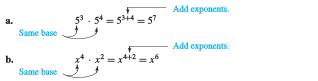
\includegraphics[width=1\linewidth]{images/fig-product-of-powers}
%
\end{example}
\par
Here are some mistakes to avoid.%
\begin{warning}[]\label{warning-5}
\leavevmode%
\begin{enumerate}[label=*\arabic**]
\item\hypertarget{li-187}{}Note that we do not \emph{multiply} the exponents when simplifying a product. For example,%
\begin{equation*}
b^4 \cdot b^2 \ne b^8
\end{equation*}
You can check this with your calculator by choosing a value for \(b\), for instance, \(b = 3\):%
\begin{equation*}
3^4 \cdot 3^2\ne 3^8
\end{equation*}
%
\item\hypertarget{li-188}{}In order to apply the first law of exponents, the bases must be the same. For example,%
\begin{equation*}
2^3 \cdot 3^5 \ne 6^8
\end{equation*}
(Check this on your calculator.)%
\item\hypertarget{li-189}{}We do not multiply the bases when simplifying a product. In \hyperref[example-product-of-powers]{Example~\ref{example-product-of-powers}}a, note that%
\begin{equation*}
5^3 \cdot 5^4\ne 25^7
\end{equation*}
%
\item\hypertarget{li-190}{}Although we can simplify the product \(x^2x^3\) as \(x^5\), we cannot simplify the sum \(x^2 + x^3\), because \(x^2\) and \(x^3\) are not like terms.%
\end{enumerate}
%
\end{warning}
\begin{example}[]\label{example-34}
Multiply \((−3x^4z^2) (5x^3 z)\).%
\par\medskip\noindent%
\textbf{Solution.}\quad Rearrange the factors to group the numerical coefficients and the powers of each base. Apply the first law of exponents.%
\begin{align*}
(−3x^4z^2) (5x^3z) \amp = (−3) (5)x^4x^3z^2z\\
\amp = -15x^7z^3
\end{align*}
%
\end{example}
\typeout{************************************************}
\typeout{Subsection A.6.2 Quotients of Powers}
\typeout{************************************************}
\subsection[{Quotients of Powers}]{Quotients of Powers}\label{subsection-22}
To reduce a fraction, we divide both numerator and denominator by any common factors.%
\begin{equation*}
\require{cancel} \require{color} \renewcommand{\CancelColor}{\blue}
\frac{x^7}{x^4}=\frac{xxx\cancel{x}\cancel{x}\cancel{x}\cancel{x}}{\cancel{x}\cancel{x}\cancel{x}\cancel{x}}=\frac{x^3}{1}=x^3
\end{equation*}
We can obtain the same result more quickly by \emph{subtracting} the exponent of the denominator from the exponent of the numerator.%
\begin{equation*}
\frac{x^7}{x^4}=x^{7-4}=x^3
\end{equation*}
%
\par
What if the larger power occurs in the denominator of the fraction?%
\begin{equation*}
\frac{x^4}{x^7}=\frac{\cancel{x}\cancel{x}\cancel{x}\cancel{x}}{xxx\cancel{x}\cancel{x}\cancel{x}\cancel{x}}=\frac{1}{x^3}
\end{equation*}
In this case, we subtract the exponent of the numerator from the exponent of the denominator.%
\begin{equation*}
\frac{x^4}{x^7}=\frac{1}{x^{7-4}}=\frac{1}{x^3}
\end{equation*}
These examples suggest the following law.%
\begin{assemblage}{Second Law of Exponents: Quotient of Powers}\label{assemblage-16}
To divide two powers with the same base, subtract the smaller exponent from the larger one, keeping the same base. \leavevmode%
\begin{enumerate}
\item\hypertarget{li-191}{}If the larger exponent occurs in the numerator, put the power in the numerator.%
\begin{equation*}
\text{If }m\gt n,~\text{ then }~ \frac{a^m}{a^n}=a^{m-n} \hphantom{blank}(a \ne 0)
\end{equation*}
%
\item\hypertarget{li-192}{}If the larger exponent occurs in the denominator, put the power in the denominator.%
\begin{equation*}
\text{If }m\lt n,~\text{ then }~ \frac{a^m}{a^n}=\frac{1}{a^{n-m}} \hphantom{blank}(a \ne 0)
\end{equation*}
%
\end{enumerate}
%
\end{assemblage}
\begin{example}[]\label{example-35}
\leavevmode%
\begin{enumerate}
\item\hypertarget{li-193}{}\(\dfrac{3^8}{3^2}=3^{8-2}=3^6\hphantom{blankblankbla}\text{Subtract exponents: }~8 \gt 2.\)%
\item\hypertarget{li-194}{}\(\displaystyle{\frac{w^3}{w^6}=\frac{1}{w^{6-3}}=\frac{1}{w^3}\hphantom{blankblank}\text{Subtract exponents: }3\lt 6.}\)%
\end{enumerate}
%
\end{example}
\begin{example}[]\label{example-36}
Divide \(\dfrac{3x^2 y^4}{6x^3 y}.\)%
\par\medskip\noindent%
\textbf{Solution.}\quad Consider the numerical coefficients and the powers of each variable separately. Use the second law of exponents to simplify each quotient of powers.%
\begin{align*}
\frac{3x^2 y^4}{6x^3 y} \amp = \frac{3}{6}\cdot \frac{x^2}{x^3} \cdot \frac{y^4}{y}\amp\amp\text{Subtract exponents.}
\\
\amp = \frac{1}{2}\cdot \frac{1}{x^{3-2}} \cdot y^{4-1}\\
\amp = \frac{1}{2}\cdot \frac{1}{x} \cdot y^3=\frac{y^3}{2x}
\end{align*}
%
\end{example}
\typeout{************************************************}
\typeout{Subsection A.6.3 Power of a Power}
\typeout{************************************************}
\subsection[{Power of a Power}]{Power of a Power}\label{subsection-23}
Consider the expression \(\left(a^4\right)^3\), the third power of \(a^4\).%
\begin{equation*}
\left(a^4\right)^3=\left(a^4\right)\left(a^4\right)\left(a^4\right)
=a^{4+4+4}=a^{12} \hphantom{blankblankblank}\text{Add exponents.}
\end{equation*}
We can obtain the same result by multiplying the exponents together.%
\begin{equation*}
\left(a^4\right)^3=a^{4 \,\cdot\, 3}=a^{12}
\end{equation*}
%
\begin{assemblage}{Third Law of Exponents: Power of a Power}\label{assemblage-17}
To raise a power to a power, keep the same base and multiply the exponents.%
\begin{equation*}
\left(a^m\right)^n = a^{mn}
\end{equation*}
%
\end{assemblage}
\begin{example}[]\label{example-37}
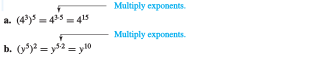
\includegraphics[width=1\linewidth]{images/fig-power-of-power}
%
\end{example}
\begin{warning}[]\label{warning-6}
Notice the difference between the expressions%
\begin{equation*}
(x^3) (x^4) = x^{3+4} = x^7
\end{equation*}
and%
\begin{equation*}
\left(x^3\right)^4 = x^{3\, \cdot \, 4} = x^{12}
\end{equation*}
The first expression is a product, so we add the exponents. The second expression raises a power to a power, so we multiply the exponents.%
\end{warning}
\typeout{************************************************}
\typeout{Subsection A.6.4 Power of a Product}
\typeout{************************************************}
\subsection[{Power of a Product}]{Power of a Product}\label{subsection-24}
To simplify the expression \((5a)^3\), we use the associative and commutative laws to regroup the factors as follows.%
\begin{align*}
(5a)^3 \amp = (5a) (5a) (5a)
\\
\amp =  5 \cdot 5 \cdot 5 \cdot a \cdot a \cdot a
\\
\amp = 5^3 a^3
\end{align*}
Thus, to raise a product to a power, we can simply raise each factor to the power.%
\begin{assemblage}{Fourth Law of Exponents: Power of a Product}\label{assemblage-18}
A power of a product is equal to the product of the powers of each of its factors.%
\begin{equation*}
(ab)^n = a^n b^n
\end{equation*}
%
\end{assemblage}
\begin{example}[]\label{example-38}
\leavevmode%
\begin{enumerate}[label=*\alph**]
\item\hypertarget{li-195}{}\((5a)^3 = 5^3a^3 = 125a^3\hphantom{blank}\text{Cube each factor}\).%
\item\hypertarget{li-196}{}\(\begin{aligned}
\left(−xy^2\right)^4\amp = (−x)^4\left(y^2\right)^4 \amp\amp\text{Raise each factor to the fourth power.}\\
\amp =x^4y^8\amp\amp\text{Apply the third law of exponents.}
\end{aligned}\)%
\end{enumerate}
%
\end{example}
\begin{warning}[]\label{warning-7}
\leavevmode%
\begin{enumerate}[label=*\arabic**]
\item\hypertarget{li-197}{}Compare the two expressions \(3a^2\) and \((3a)^2\); they are not the same. In the expression \(3a^2\), only the factor \(a\) is squared. But in \((3a)^2\), both \(3\) and \(a\) are squared. Thus,%
\begin{equation*}
3a^2 ~~\text{  cannot be simplified}
\end{equation*}
but%
\begin{equation*}
(3a)^2 = 3^2a^2 = 9a^2
\end{equation*}
%
\item\hypertarget{li-198}{}Compare the two expressions \((3a)^2\) and \((3 + a)^2\). The fourth law of exponents applies to the \emph{product} \(3a\), but not to the \emph{sum} \(3+a\). Thus,%
\begin{equation*}
(3 + a)^2 \ne 3^2 + a^2
\end{equation*}
In order to simplify \((3 + a)^2\), we must expand the binomial product:%
\begin{equation*}
(3 + a)^2 = (3 + a) (3 + a) = 9 + 6a + a^2
\end{equation*}
%
\end{enumerate}
%
\end{warning}
\typeout{************************************************}
\typeout{Subsection A.6.5 Power of a Quotient}
\typeout{************************************************}
\subsection[{Power of a Quotient}]{Power of a Quotient}\label{subsection-25}
To simplify the expression \(\displaystyle{\left(\frac{x}{3}\right)^4} \), we multiply together \(4\) copies of the fraction \(\dfrac{x}{3}\).%
\begin{align*}
\left(\frac{x}{3}\right)^4 \amp = \frac{x}{3}\cdot \frac{x}{3}\cdot \frac{x}{3}\cdot \frac{x}{3}
= \frac{x\cdot x\cdot x\cdot x}{3\cdot 3\cdot 3\cdot 3}
\\
\amp = \frac{x^4}{3^4}=\frac{x^4}{81}
\end{align*}
In general, we have the following rule.%
\begin{assemblage}{Fifth Law of Exponents: Power of a Quotient}\label{assemblage-19}
To raise a quotient to a power, raise both the numerator and denominator to the power.%
\begin{equation*}
\left(\frac{a}{b}\right)^n=\frac{a^n}{b^n}
\end{equation*}
%
\end{assemblage}
\par
For reference, we state all of the laws of exponents together. All the laws are valid when a and b are not equal to zero and when the exponents m and n are whole numbers.%
\begin{assemblage}{Laws of Exponents}\label{assemblage-20}
\leavevmode%
\begin{enumerate}[label=*\Roman**]
\item\hypertarget{li-199}{}\(a^m\cdot a^n = a^{m+n}\)%
\item\hypertarget{li-200}{}%
\begin{enumerate}[label=*\alph**]
\item\hypertarget{li-201}{}\(\dfrac{a^m}{a^n}=a^{m-n} \hphantom{blank}m\gt n\)%
\item\hypertarget{li-202}{}\(\displaystyle{\frac{a^m}{a^n}=\frac{1}{a^{n-m}} \hphantom{blank}m\lt n}\)%
\end{enumerate}
%
\item\hypertarget{li-203}{}\(\left(a^m\right)^n=a^{m+n}\)%
\item\hypertarget{li-204}{}\((ab)^n=a^n b^n\)%
\item\hypertarget{li-205}{}\(\displaystyle{\left(\frac{a}{b}\right)^n = \frac{a^n}{b^n} }\)%
\end{enumerate}
%
\end{assemblage}
\begin{example}[]\label{example-39}
Simplify \(5x^2 y^3\left(2xy^2\right)^4\).%
\par\medskip\noindent%
\textbf{Solution.}\quad According to the order of operations, we should perform any powers before multiplications. Thus, we begin by simplifying \((2xy^2)^4\). We apply the fourth law.%
\begin{align*}
5x^2 y^3\left(2xy^2\right)^4 \amp = 5x^2 y^3 · 2^4x^4\left(y^2\right)^4 \amp\amp\text{Apply the fourth law.}
\\
\amp = 5x^2 y^3 · 2^4x^4 y^8
\end{align*}
Finally, multiply powers with the same base. Apply the first law.%
\begin{equation*}
5x^2 y^3 \cdot 2^4x^4 y^8 = 5 \cdot 2^4 x^2x^4 y^3 y^8 = 80x^6 y^{11}
\end{equation*}
%
\end{example}
\begin{example}[]\label{example-40}
Simplify \(\displaystyle{\left(\frac{2x}{z^2}\right)^3}\).%
\par\medskip\noindent%
\textbf{Solution.}\quad Begin by applying the fifth law.%
\begin{align*}
\require{\stackengine}
\left(\frac{2x}{z^2}\right)^3 \amp = \frac{(2x)^3}{\left(z^2\right)^2}\amp\amp
{\text{Apply the fourth law to the numerator }}{\text{and the third law to the denominator.}}
\\
\amp = \frac{2^3x^3}{z^6}=\frac{8x^3}{z^6}
\end{align*}
%
\end{example}
\typeout{************************************************}
\typeout{Section A.7 Polynomials and Factoring}
\typeout{************************************************}
\section[{Polynomials and Factoring}]{Polynomials and Factoring}\label{appendix-Polynomials-and-Factoring}
In \hyperref[appendix-Laws-of-Exponents]{Section~\ref{appendix-Laws-of-Exponents}}, we used the first law of exponents to multiply two or more monomials. In this section, we review techniques for multiplying and factoring polynomials of several terms.%
\typeout{************************************************}
\typeout{Subsection A.7.1 Polynomials}
\typeout{************************************************}
\subsection[{Polynomials}]{Polynomials}\label{subsection-26}
A \terminology{polynomial} is a sum of terms in which all the exponents on the variables are whole numbers and no variables appear in the denominator or under a radical. The expressions%
\begin{equation*}
0.1 R^4, ~~d^2 + 32 d − 21, ~~\text{ and }~~128x^3 − 960x^2 + 8000
\end{equation*}
are all examples of polynomials in one variable.%
\par
An algebraic expression consisting of one term of the form \(cx^n\), where \(c\) is a constant and \(n\) is a whole number, is called a \terminology{monomial}. For example,%
\begin{equation*}
y3, ~~−3x^8, ~~\text{ and } ~~0.1R^4
\end{equation*}
are monomials. A polynomial is just a sum of one or more monomials.%
\par
A polynomial with exactly two terms, such as \(\frac{1}{2}n^2 + \frac{1}{2}n\), is called a \terminology{binomial}. A polynomial with exactly three terms, such as \(d^2 + 32 d − 21\) or \(128x^3 − 960x^2 + 8000\), is called a \terminology{trinomial}. We have no special names for polynomials with more than three terms.%
\begin{example}[]\label{example-41}
Which of the following expressions are polynomials? \leavevmode%
\begin{enumerate}[label=*\alph**]
\item\hypertarget{li-206}{}\(\pi r^2\)%
\item\hypertarget{li-207}{}\(23.4s^6 − 47.9s^4\)%
\item\hypertarget{li-208}{}\(\frac{2}{3}w^3 − \frac{7}{3}w^2 + \frac{1}{3}w\)%
\item\hypertarget{li-209}{}\(7 + m^{−2}\)%
\item\hypertarget{li-210}{}\(\frac{x-2}{x+2}\)%
\item\hypertarget{li-211}{}\(\sqrt[3]{4y}\)%
\end{enumerate}
%
\par\medskip\noindent%
\textbf{Solution.}\quad The first three are all polynomials. In fact, (a) is a monomial, (b) is a binomial, and (c) is a trinomial. The last three are not polynomials. The variable in (d) has a negative exponent, the variable in (e) occurs in the denominator, and the variable in (f) occurs under a radical.%
\end{example}
\par
In a polynomial containing only one variable, the greatest exponent that appears on the variable is called the \terminology{degree} of the polynomial. If there is no variable at all, then the polynomial is called a constant, and the degree of a constant is zero.%
\begin{example}[]\label{example-42}
Give the degree of each polynomial. \leavevmode%
\begin{enumerate}[label=*\alph**]
\item\hypertarget{li-212}{}\(b^3 − 3b^2 + 3b − 1\)%
\item\hypertarget{li-213}{}\(10^{10}\)%
\item\hypertarget{li-214}{}\(−4w^3\)%
\item\hypertarget{li-215}{}\(s^2 − s^6\)%
\end{enumerate}
%
\par\medskip\noindent%
\textbf{Solution.}\quad \leavevmode%
\begin{enumerate}[label=*\alph**]
\item\hypertarget{li-216}{}This is a polynomial in the variable \(b\), and because the greatest exponent on \(b\) is \(3\), the degree of this polynomial is \(3\).%
\item\hypertarget{li-217}{}This is a constant polynomial, so its degree is \(0\). (The exponent on a constant does not affect the degree.)%
\item\hypertarget{li-218}{}This monomial has degree \(3\).%
\item\hypertarget{li-219}{}This is a binomial of degree \(6\).%
\end{enumerate}
%
\end{example}
\par
We can evaluate a polynomial just as we evaluate any other algebraic expression: We replace the variable with a number and simplify the result.%
\begin{example}[]\label{example-43}
Let \(p(x) = −2x^2 + 3x − 1\). Evaluate each of the following. \leavevmode%
\begin{enumerate}[label=*\alph**]
\item\hypertarget{li-220}{}\(p(2)\)%
\item\hypertarget{li-221}{}\(p(-1)\)%
\item\hypertarget{li-222}{}\(p(t)\)%
\item\hypertarget{li-223}{}\(p(t+3)\)%
\end{enumerate}
%
\par\medskip\noindent%
\textbf{Solution.}\quad In each case, we replace \(x\) by the given value. \leavevmode%
\begin{enumerate}[label=*\alph**]
\item\hypertarget{li-224}{}\(p(\alert{2})=−2(\alert{2})^2 + 3(\alert{2}) − 1=-8+6-1=-3\)%
\item\hypertarget{li-225}{}\(p(\alert{-1})=−2(\alert{-1})^2 + 3(\alert{-1}) − 1=-2+(-3)-1=-6\)%
\item\hypertarget{li-226}{}\(p(\alert{t})=−2(\alert{t})^2 + 3(\alert{t}) − 1=--2t^2+3t-1\)%
\item\hypertarget{li-227}{}\(\begin{aligned}
\amp \\
p(\alert{t+3})\amp =−2(\alert{t+3})^2 + 3(\alert{t+3}) − 1\\
\amp = -2(t^2+6t+9)+3(t+3)-1\\
\amp = -2t^2-9t-10
\end{aligned}\)%
\end{enumerate}
%
\end{example}
\typeout{************************************************}
\typeout{Subsection A.7.2 Products of Polynomials}
\typeout{************************************************}
\subsection[{Products of Polynomials}]{Products of Polynomials}\label{subsection-27}
To multiply polynomials, we use a generalized form of the distributive property:%
\begin{equation*}
a(b + c + d + \cdots) = ab + ac + ad + \cdots
\end{equation*}
To multiply a polynomial by a monomial, we multiply each term of the polynomial by the monomial.%
\begin{example}[]\label{example-44}
\leavevmode%
\begin{enumerate}[label=*\alph**]
\item\hypertarget{li-228}{}\(\begin{aligned}
\amp\\
3x(x + y + z) \amp = 3x(x) + 3x(y) + 3x(z)\\
\amp = 3x^2+3xy+3xz
\end{aligned}\)%
\item\hypertarget{li-229}{}\(\begin{aligned}
\amp\\
−2ab^2(3a^2 − ab + 2b^2) \amp = −2ab^2(3a^2) − 2ab^2(−ab) − 2ab^2(2b^2)\\
\amp = -6a^3b^2+2a^2b^3-4ab^4
\end{aligned}\)%
\end{enumerate}
%
\end{example}
\typeout{************************************************}
\typeout{Subsection A.7.3 Products of Binomials}
\typeout{************************************************}
\subsection[{Products of Binomials}]{Products of Binomials}\label{subsection-28}
Products of binomials occur so frequently that it is worthwhile to learn a shortcut for this type of multiplication. We can use the following scheme to perform the multiplication mentally. (See \hyperref[fig-FOIL]{Figure~\ref{fig-FOIL}}.) \leavevmode%
\begin{figure}
\centering
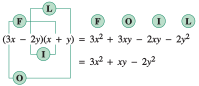
\includegraphics[width=0.6\linewidth]{images/fig-FOIL}
\caption{\label{fig-FOIL}}
\end{figure}
%
\begin{example}[]\label{example-45}
%
\begin{align*}
(2x − 1)(x + 3) \amp = 2x^2 + 6x − x − 3\\
\amp = 2x^2 + 5x − 3
\end{align*}
%
\end{example}
\typeout{************************************************}
\typeout{Subsection A.7.4 Factoring}
\typeout{************************************************}
\subsection[{Factoring}]{Factoring}\label{subsection-29}
We sometimes find it useful to write a polynomial as a single \emph{term} composed of two or more \emph{factors}. This process is the reverse of multiplication and is called \terminology{factoring}. For example, observe that%
\begin{equation*}
3x^2 + 6x = 3x(x + 2)
\end{equation*}
We will only consider factorization in which the factors have integer coefficients.%
\typeout{************************************************}
\typeout{Subsection A.7.5 Common Factors}
\typeout{************************************************}
\subsection[{Common Factors}]{Common Factors}\label{subsection-30}
We can factor a common factor from a polynomial by using the distributive property in the form%
\begin{equation*}
ab + ac = a(b + c)
\end{equation*}
We first identify the common factor. For example, each term of the polynomial%
\begin{equation*}
6x^3 + 9x^2 − 3x
\end{equation*}
contains the monomial \(3x\) as a factor; therefore,%
\begin{equation*}
6x^3 + 9x^2 − 3x = 3x (\fillin{6.818181818181818})
\end{equation*}
Next, we insert the proper polynomial factor within the parentheses. This factor can be determined by inspection. We ask ourselves for monomials that, when multiplied by \(3x\), yield \(6x^3\), \(9x^2\), and \(−3x\), respectively, and obtain%
\begin{equation*}
6x^3 + 9x^2 − 3x = 3x(2x^2 + 3x − 1)
\end{equation*}
%
\par
We can check the result of factoring an expression by multiplying the factors. In the example above,%
\begin{equation*}
3x(2x^2 + 3x − 1) = 6x^3 + 9x^2 − 3x
\end{equation*}
%
\begin{example}[]\label{example-46}
\leavevmode%
\begin{enumerate}[label=*\alph**]
\item\hypertarget{li-230}{}\(\begin{aligned} \\
18x^2 y − 24xy2 \amp = 6xy(\text{?} - \text{?}) \\
\amp = 6xy(3x − 4y)
\end{aligned}\)%
\par
because%
\begin{equation*}
6xy(3x − 4y) = 18x^2 y − 24xy^2
\end{equation*}
%
\item\hypertarget{li-231}{}\(\begin{aligned} \\
y(x − 2) + z(x − 2) \amp = (x − 2)(\text{?} - \text{?}) \\
\amp = (x − 2)(y + z)
\end{aligned}\)%
\par
because%
\begin{equation*}
(x − 2)(y + z) = y(x − 2) + z(x − 2)
\end{equation*}
%
\end{enumerate}
%
\end{example}
\typeout{************************************************}
\typeout{Subsection A.7.6 Opposite of a Binomial}
\typeout{************************************************}
\subsection[{Opposite of a Binomial}]{Opposite of a Binomial}\label{subsection-31}
It is often useful to factor \(-1\) from the terms of a binomial.%
\begin{align*}
a − b \amp = (−1)(−a + b)
\\
\amp = (−1)(b − a) = −(b − a)
\end{align*}
Hence, we have the following important relationship.%
\begin{assemblage}{Opposite of a Binomial}\label{assemblage-21}
%
\begin{equation*}
a-b=-(b-a)
\end{equation*}
%
\end{assemblage}
\par
That is, \(a-b\) and \(b-a\) are opposites or negatives of each other.%
\begin{example}[]\label{example-47}
\leavevmode%
\begin{enumerate}[label=*\alph**]
\item\hypertarget{li-232}{}\(3x − y = −(y − 3x)\)%
\item\hypertarget{li-233}{}\(a − 2b = −(2b − a)\)%
\end{enumerate}
%
\end{example}
\typeout{************************************************}
\typeout{Subsection A.7.7 Polynomial Division}
\typeout{************************************************}
\subsection[{Polynomial Division}]{Polynomial Division}\label{subsection-32}
We can divide one polynomial by a polynomial of lesser degree. The quotient will be the sum of a polynomial and a simpler algebraic fraction.%
\par
If the divisor is a monomial, we can simply divide the monomial into each term of the numerator.%
\begin{example}[]\label{example-48}
Divide \(\dfrac{9x^3 − 6x^2 + 4}{3x}\)%
\par\medskip\noindent%
\textbf{Solution.}\quad Divide \(3x\) into each term of the numerator.%
\begin{align*}
\frac{9x^3 − 6x^2 + 4}{3x} \amp = \frac{9x^3}{3x}− \frac{6x^2}{3x}+ \frac{4}{3x}
\\
\amp = 3x^2 − 2x + \frac{4}{3x}
\end{align*}
The quotient is the sum of a polynomial, \(3x^2 − 2x\), and an algebraic fraction, \(\frac{4}{3x}\).%
\end{example}
\par
If the denominator is not a monomial, we can use a method similar to the long division algorithm used in arithmetic.%
\begin{example}[]\label{example-long-division}
Divide \(\dfrac{2x^2+x-7}{x+3}\)%
\par\medskip\noindent%
\textbf{Solution.}\quad First write \leavevmode%
\begin{figure}
\centering
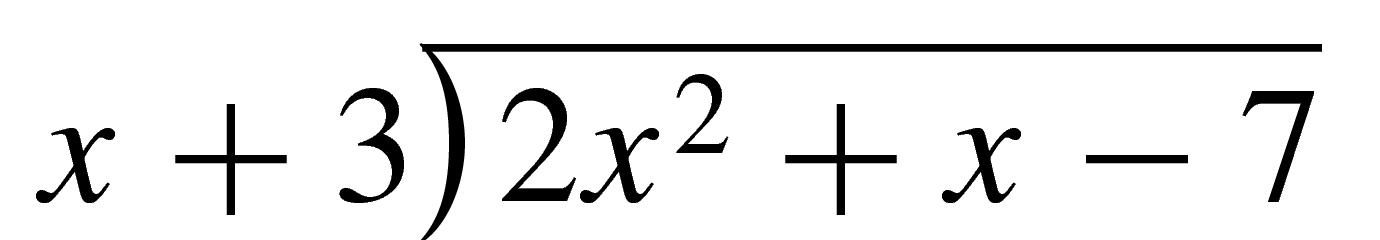
\includegraphics[width=0.35\linewidth]{images/fig-long-division.jpg}
\end{figure}
 and divide \(2x^2\) (the first term of the numerator) by \(x\) (the first term of the denominator) to obtain \(2x\). (It may be helpful to write down the division: \(\frac{2x^2}{2x}=x\).) Write \(2x\) above the quotient bar as the first term of the quotient, as shown below.%
\par
Next, multiply \(x+3\) by \(2x\) to obtain \(2x^2 + 6x\), and subtract this product from \(2x^2 + x − 7\): \leavevmode%
\begin{figure}
\centering
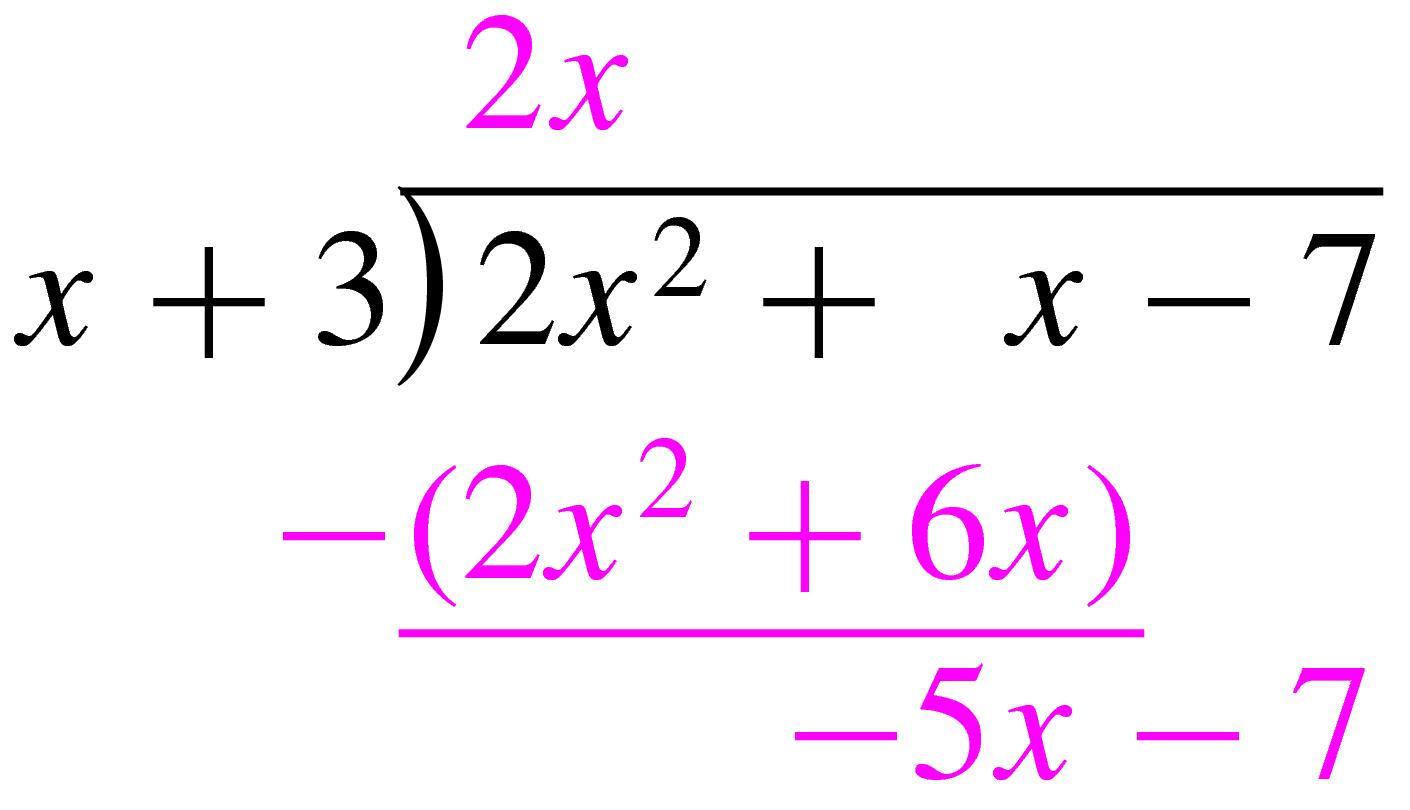
\includegraphics[width=0.35\linewidth]{images/fig-long-division2.jpg}
\end{figure}
%
\par
Repeating the process, divide \(-5x\) by \(x\) to obtain \(-5\). Write \(-5\) as the second term of the quotient. Then multiply \(x+3\) by \(-5\) to obtain \(−5x − 15\), and subtract: \leavevmode%
\begin{figure}
\centering
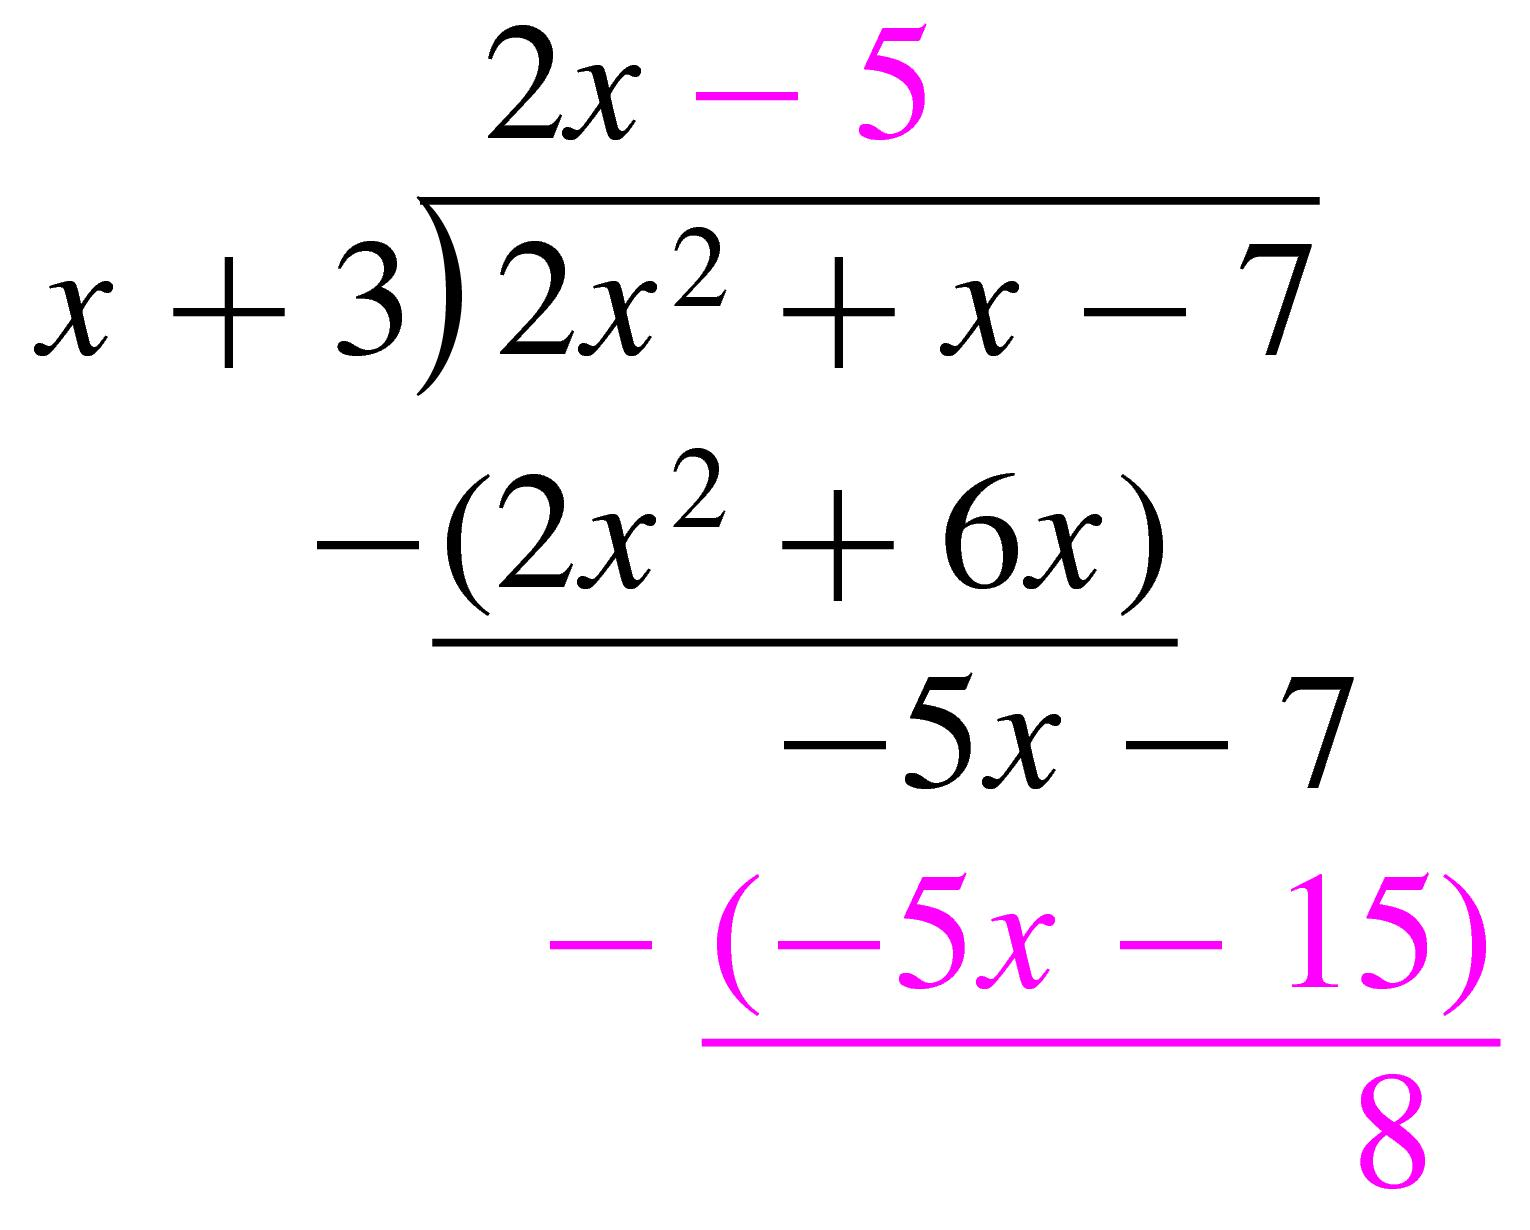
\includegraphics[width=0.35\linewidth]{images/fig-long-division3.jpg}
\end{figure}
 Because the degree of \(8\) is less than the degree of \(x + 3\), the division is finished. The quotient is \(2x − 5\), with a remainder of \(8\). We write the remainder as a fraction to obtain%
\begin{equation*}
\frac{2x^2 + x − 7}{x + 3}= 2x − 5 + \frac{8}{x + 3}
\end{equation*}
%
\end{example}
\par
When using polynomial division, it helps to write the polynomials in descending powers of the variable. If the numerator is missing any terms, we can insert terms with zero coefficients so that like powers will be aligned. For example, to perform the division%
\begin{equation*}
\frac{3x − 1 + 4x^3}{2x-1}
\end{equation*}
we first write the numerator in descending powers as \(4x^3 + 3x − 1\). We then insert \(0x^2\) between \(4x^3\) and \(3x\) and set up the quotient as \leavevmode%
\begin{figure}
\centering
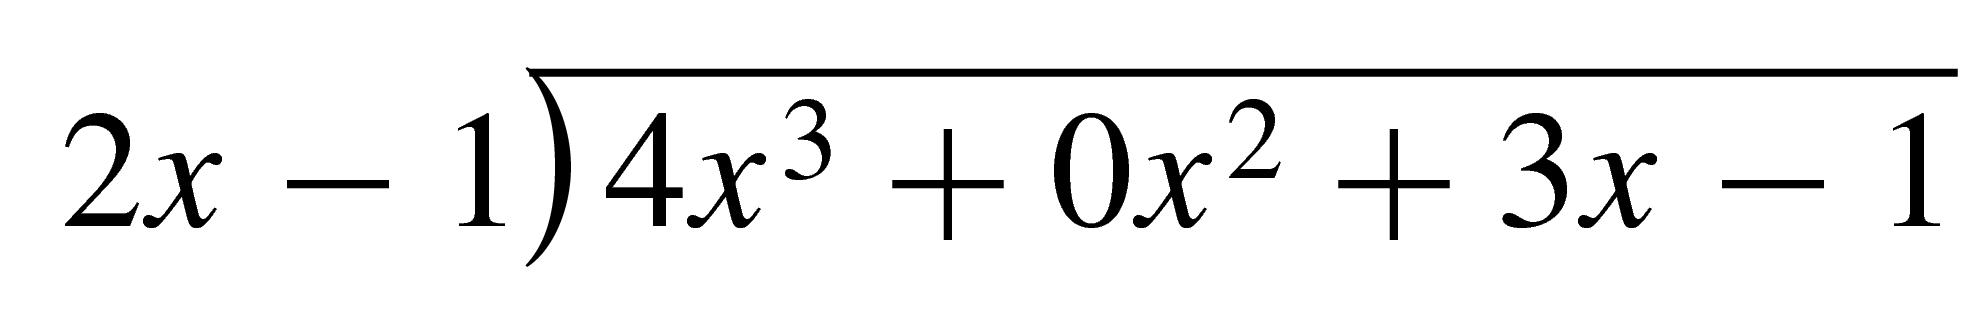
\includegraphics[width=0.38\linewidth]{images/fig-long-division4.jpg}
\end{figure}
 We then proceed as in \hyperref[example-long-division]{Example~\ref{example-long-division}}. You can check that the quotient is%
\begin{equation*}
2x^2 + x + 2 + \frac{1}{2x-1}
\end{equation*}
%
\typeout{************************************************}
\typeout{Section A.8 Factoring Quadratic Trinomials}
\typeout{************************************************}
\section[{Factoring Quadratic Trinomials}]{Factoring Quadratic Trinomials}\label{appendix-Factoring-Quadratic-Trinomials}
Consider the trinomial%
\begin{equation*}
x^2 + 10x + 16
\end{equation*}
Can we find two binomial factors,%
\begin{equation*}
(x + a)(x + b)
\end{equation*}
whose product is the given trinomial? The product of the binomials is%
\begin{equation*}
(x + a)(x + b) = x^2 + (a + b)x + ab
\end{equation*}
Thus, we are looking for two numbers, a and b, that satisfy%
\begin{equation*}
(x + a)(x + b) = x^2 + (a + b)x + ab
\end{equation*}
%
\begin{equation*}
(x + a)(x + b) = x^2 + (a + b)x + ab= x^2 + 10x + 16
\end{equation*}
By comparing the coefficients of the terms in the two trinomials, we see that \(a + b = 10\) and \(ab = 16\). That is, the sum of the two numbers is the coefficient of the linear term, \(10\), and their product is the constant term, \(16\).%
\par
To find the numbers, we list all the possible integer factorizations of \(16\):%
\begin{equation*}
1 \cdot 16, ~~~2 \cdot 8, ~~~\text{ and }~~~ 4 \cdot 4
\end{equation*}
We see that only one combination gives the correct linear term: \(8\) and \(2\). These are the numbers \(a\) and \(b\), so%
\begin{equation*}
x^2 + 10x + 16 = (x + 8)(x + 2)
\end{equation*}
%
\par
In \hyperref[example-factor-trinomial]{Example~\ref{example-factor-trinomial}} we factor quadratic trinomials in which one or more of the coefficients is negative.%
\begin{example}[]\label{example-factor-trinomial}
Factor. \leavevmode%
\begin{enumerate}[label=*\alph**]
\item\hypertarget{li-234}{}\(x^2-7x+12\)%
\item\hypertarget{li-235}{}\(x^2-x-12\)%
\end{enumerate}
%
\par\medskip\noindent%
\textbf{Solution.}\quad \leavevmode%
\begin{enumerate}[label=*\alph**]
\item\hypertarget{li-236}{}Find two numbers whose product is \(12\) and whose sum is \(-7\). Because the product is positive and the sum is negative, the two numbers must both be negative. The possible factors of \(12\) are \(-1\) and \(-12\), \(-2\) and \(-6\), or \(-3\) and \(-4\). Only \(-4\) and \(-3\) have the correct sum, \(-7\). Hence,%
\begin{equation*}
x^2 − 7x + 12 = (x − 4) (x − 3)
\end{equation*}
%
\item\hypertarget{li-237}{}Find two numbers whose product is \(-12\) and whose sum is \(-1\). Because the product is negative, the two numbers must be of opposite sign and their sum must be \(-1\). By listing the possible factors of \(-12\), we find that the two numbers are \(-4\) and \(3\). Hence,%
\begin{equation*}
x^2 − x − 12 = (x − 4) (x + 3)
\end{equation*}
%
\end{enumerate}
%
\end{example}
\par
If the coefficient of the quadratic term is not \(1\), we must also consider its factors.%
\begin{example}[]\label{example-51}
Factor \(8x^2 − 9 − 21x\).%
\par\medskip\noindent%
\textbf{Solution.}\quad \leavevmode%
\begin{description}
\item[{Step 1}]\hypertarget{li-238}{}Write the trinomial in decreasing powers of \(x\).%
\begin{equation*}
8x^2-21x-9
\end{equation*}
%
\item[{Step 2}]\hypertarget{li-239}{}List the possible factors for the quadratic term.%
\begin{align*}
(8x\hphantom{00000})\amp(x\hphantom{000000})\\
(4x\hphantom{00000})\amp(2x\hphantom{00000})
\end{align*}
%
\item[{Step 3}]\hypertarget{li-240}{}Consider possible factors for the constant term: \(9\) may be factored as \(9\cdot 1\) or as \(3\cdot 3\). Form all possible pairs of binomial factor using these factorizations. (See \hyperref[fig-factor-trinomial]{Figure~\ref{fig-factor-trinomial}}.) \leavevmode%
\begin{figure}
\centering
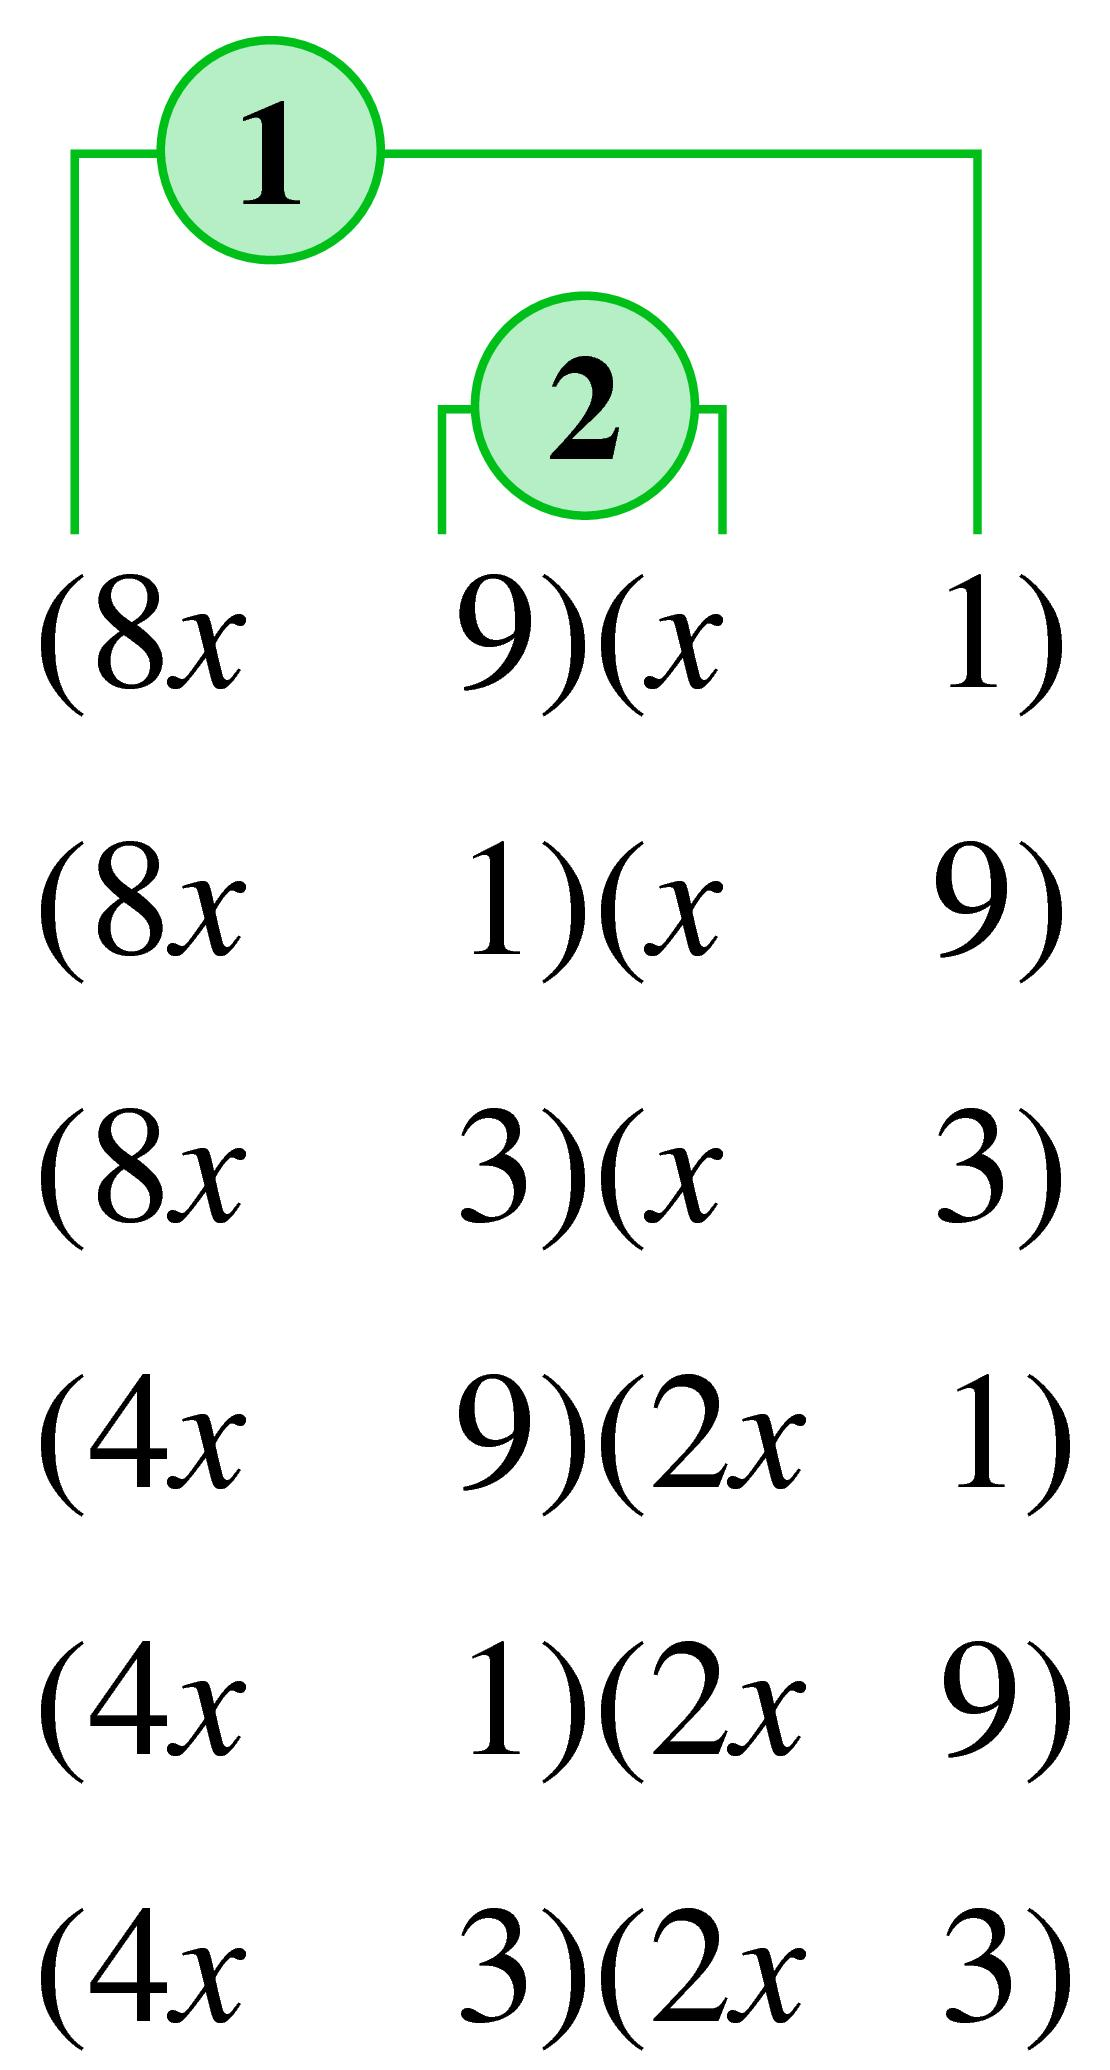
\includegraphics[width=0.4\linewidth]{images/fig-factor-trinomial.jpg}
\caption{\label{fig-factor-trinomial}}
\end{figure}
%
\item[{Step 4}]\hypertarget{li-241}{}Select the combinations of the products ❶ and ❷ whose sum or difference could be the linear term, \(-21x\).%
\begin{equation*}
(8x \hphantom{000} 3) (x \hphantom{000} 3)
\end{equation*}
%
\item[{Step 5}]\hypertarget{li-242}{}Insert the proper signs:%
\begin{equation*}
(8x + 3) (x − 3)
\end{equation*}
%
\end{description}
%
\end{example}
\par
With practice, you can usually factor trinomials of the form \(Ax^2 + Bx + C\) mentally. The following observations may help. \leavevmode%
\begin{enumerate}[label=*\arabic**]
\item\hypertarget{li-243}{}If \(A\), \(B\) and \(C\) are all positive, both signs in the factored form are positive. For example, as a first step in factoring \(6x^2 + 11x + 4\), we could write%
\begin{equation*}
(\hphantom{000} + \hphantom{000} ) (\hphantom{000}  + \hphantom{000} )
\end{equation*}
%
\item\hypertarget{li-244}{}If \(A\) and \(C\) are positive and \(B\) is negative, both signs in the factored form are negative. Thus as a first step in factoring \(6x^2 − 11x + 4\), we could write%
\begin{equation*}
(\hphantom{000} - \hphantom{000} ) (\hphantom{000}  - \hphantom{000} )
\end{equation*}
%
\item\hypertarget{li-245}{}If \(C\) is negative, the signs in the factored form are opposite. Thus as a first step in factoring \(6x^2 − 5x − 4\), we could write%
\begin{equation*}
(\hphantom{000} + \hphantom{000} ) (\hphantom{000}  - \hphantom{000} )
~~\text{ or }~~  (\hphantom{000} - \hphantom{000} ) (\hphantom{000}  + \hphantom{000} )
\end{equation*}
%
\end{enumerate}
%
\begin{example}[]\label{example-52}
\leavevmode%
\begin{enumerate}[label=*\alph**]
\item\hypertarget{li-246}{}\(\begin{aligned}
6x^2 + 5x + 1 \amp = \hphantom{000} + \hphantom{000} ) (\hphantom{000}  + \hphantom{000} )\\
\amp = (3x + 1) (2x + 1)
\end{aligned}\)%
\item\hypertarget{li-247}{}\(\begin{aligned}
6x^2 − 5x + 1 \amp = (\hphantom{000} - \hphantom{000} ) (\hphantom{000}  - \hphantom{000} )\\
\amp =  (3x − 1) (2x − 1)
\end{aligned}\)%
\item\hypertarget{li-248}{}\(\begin{aligned}
6x^2 − x - 1 \amp = (\hphantom{000} + \hphantom{000} ) (\hphantom{000}  - \hphantom{000} )\\
\amp =  (3x + 1) (2x − 1)
\end{aligned}\)%
\item\hypertarget{li-249}{}\(\begin{aligned}
6x^2 − xy - y^2 \amp = (\hphantom{000} + \hphantom{000} ) (\hphantom{000}  - \hphantom{000} )\\
\amp =  (3x + y) (2x − y)
\end{aligned}\)%
\end{enumerate}
%
\end{example}
\typeout{************************************************}
\typeout{Subsection A.8.1 Special Products and Factors}
\typeout{************************************************}
\subsection[{Special Products and Factors}]{Special Products and Factors}\label{subsection-33}
The products below are special cases of the multiplication of binomials. They occur so often that you should learn to recognize them on sight.%
\begin{assemblage}{Special Products}\label{assemblage-22}
\leavevmode%
\begin{enumerate}[label=*\Roman**]
\item\hypertarget{li-250}{}\((a + b)^2 = (a + b) (a + b) = a^2 + 2ab + b^2\)%
\item\hypertarget{li-251}{}\((a - b)^2 = (a - b) (a - b) = a^2 - 2ab + b^2\)%
\item\hypertarget{li-252}{}\((a + b)(a-b) =  a^2 - b^2\)%
\end{enumerate}
%
\end{assemblage}
\begin{warning}[]\label{warning-8}
Notice that in (I) \((a + b)^2 \ne a^2 + b^2\), and that in (II) \((a − b)^2\ne a^2 − b^2\). For example,%
\begin{align*}
(x + 4)^2 \amp\ne x^2 + 16, \amp\amp\text{ instead } \amp (x + 4)^2 \amp = x^2 + 8x + 16
\\
(t-5)^2 \amp\ne t^2 - 16, \amp\amp\text{ instead } \amp (t -5)^2 \amp= t^2 -10t  + 25
\end{align*}
%
\end{warning}
\begin{example}[]\label{example-53}
\leavevmode%
\begin{enumerate}[label=*\alph**]
\item\hypertarget{li-253}{}\(\begin{aligned}
3(x + 4)^2 \amp = 3(x^2 + 2 \cdot 4x + 4^2) \\
\amp = 3x^2 + 24x + 48
\end{aligned}\)%
\item\hypertarget{li-254}{}\(\begin{aligned}
(y + 5) (y − 5) \amp = y^2-5^2 \\
\amp = y^2-25
\end{aligned}\)%
\item\hypertarget{li-255}{}\(\begin{aligned}
(3x − 2y)^2 \amp = (3x)^2 − 2(3x)(2y) + (2y)^2 \\
\amp = 9x^2-12xy+4y^2
\end{aligned}\)%
\end{enumerate}
%
\end{example}
\par
Each of the formulas for special products, when viewed from right to left, also represents a special case of factoring quadratic polynomials.%
\begin{assemblage}{Special Factorizations}\label{assemblage-23}
\leavevmode%
\begin{enumerate}[label=*\Roman**]
\item\hypertarget{li-256}{}\(a^2 + 2ab + b^2=(a + b)^2\)%
\item\hypertarget{li-257}{}\(a^2 - 2ab + b^2=(a - b)^2 \)%
\item\hypertarget{li-258}{}\(a^2 - b^2=(a + b)(a-b)\)%
\item\hypertarget{li-259}{}\(a^2+b^2 ~~\text{ cannot be factored}\)%
\end{enumerate}
%
\end{assemblage}
\par
The trinomials in (I) and (II) are sometimes called \terminology{perfect-square trinomials} because they are squares of binomials. Note that the sum of two squares, \(a^2 + b^2\), cannot be factored.%
\begin{example}[]\label{example-54}
Factor. \leavevmode%
\begin{enumerate}[label=*\alph**]
\item\hypertarget{li-260}{}\(x^2 + 8x + 16\)%
\item\hypertarget{li-261}{}\(y^2 -10y + 25\)%
\item\hypertarget{li-262}{}\(4a^2 − 12ab + 9b^2\)%
\item\hypertarget{li-263}{}\(25m^2n^2 + 20mn + 4\)%
\end{enumerate}
%
\par\medskip\noindent%
\textbf{Solution.}\quad \leavevmode%
\begin{enumerate}[label=*\alph**]
\item\hypertarget{li-264}{}Because \(16\) is equal to \(4^2\) and \(8\) is equal to \(2\cdot 4\),%
\begin{align*}
x^2 + 8x + 16 \amp = x^2 − 2 \cdot 4x + 4^2\\
\amp = (x + 4)^2
\end{align*}
%
\item\hypertarget{li-265}{}Because \(25=5^2\)  and \(10=2\cdot 5\),%
\begin{align*}
y^2 − 10y + 25 \amp = y^2 − 2 \cdot 5y + 5^2\\
\amp = (y-5)^2
\end{align*}
%
\item\hypertarget{li-266}{}Because \(4a^2=(2a)^2\), \(9b^2=(3b)^2\),  and \(2ab=2(2a)(3b)\),%
\begin{align*}
4a^2 − 12ab + 9b^2 \amp = (2a)^2 − 2(2a)(3b) + (3b)^2\\
\amp = (2a-3b)^2
\end{align*}
%
\item\hypertarget{li-267}{}Because \(25m^2n^2=(5mn)^2\), \(4=2^2\),  and \(20mn=2(5mn)(2)\),%
\begin{align*}
25m^2n^2 + 20mn + 4 \amp = (5mn)^2 + 2(5mn)(2) + 2^2\\
\amp = (5mn+2)^2
\end{align*}
%
\end{enumerate}
%
\end{example}
\par
Binomials of the form \(a^2 − b^2\) are often called the \terminology{difference of two squares}.%
\begin{example}[]\label{factor-difference-of-squares}
Factor if possible. \leavevmode%
\begin{enumerate}[label=*\alph**]
\item\hypertarget{li-268}{}\(x^2 − 81\)%
\item\hypertarget{li-269}{}\(4x^2 − 9y^2\)%
\item\hypertarget{li-270}{}\(x^2 + 81\)%
\end{enumerate}
%
\par\medskip\noindent%
\textbf{Solution.}\quad \leavevmode%
\begin{enumerate}[label=*\alph**]
\item\hypertarget{li-271}{}The expression \(x^2 − 81\) is the difference of two squares, \(x^2 − 9^2\), and thus can be factored according to Special Factorization (III) above.%
\begin{align*}
x^2-81 \amp = x^2-9^2\\
\amp = (x+9)(x-9)
\end{align*}
%
\item\hypertarget{li-272}{}Because \(4x^2 − 9y^2\) can be written as \((2x)^2 −(3y)^2\),%
\begin{align*}
4x^2 − 9y^2 \amp =(2x^2)-(3y)^2 \\
\amp =(2x+3y)(2x-3y) 
\end{align*}
%
\item\hypertarget{li-273}{}The expression \(x^2 + 81\), or \(x^2 + 0x + 81\), is \emph{not} factorable, because no two real numbers have a product of \(81\) and a sum of \(0\).%
\end{enumerate}
%
\end{example}
\begin{warning}[]\label{warning-9}
\(x^2 + 81\ne (x + 9) (x + 9)\), which you can verify by multiplying%
\begin{equation*}
(x + 9) (x + 9) = x^2 + 18x + 8
\end{equation*}
%
\end{warning}
\par
The factors \(x + 9\) and \(x − 9\) in \hyperref[factor-difference-of-squares]{Example~\ref{factor-difference-of-squares}}a are called \terminology{conjugates} of each other. In general, any binomials of the form \(a+b\) and \(a-b\) are called a \terminology{conjugate pair}.%
\typeout{************************************************}
\typeout{Section A.9 Working with Algebraic Fractions}
\typeout{************************************************}
\section[{Working with Algebraic Fractions}]{Working with Algebraic Fractions}\label{appendix-Working-with-Algebraic-Fractions}
A quotient of two polynomials is called a \terminology{rational expression} or an \terminology{algebraic fraction}. Operations on algebraic fractions follow the same rules as operations on common fractions.%
\typeout{************************************************}
\typeout{Subsection A.9.1 Reducing Fractions}
\typeout{************************************************}
\subsection[{Reducing Fractions}]{Reducing Fractions}\label{subsection-34}
When we reduce an ordinary fraction such as \(\frac{24}{36}\), we are using the fundamental principle of fractions.%
\begin{assemblage}{Fundamental Principle of Fractions}\label{assemblage-24}
If we multiply or divide the numerator and denominator of a fraction by the same (nonzero) number, the new fraction is equivalent to the old one. In symbols,%
\begin{equation*}
\frac{ac}{bc}=\frac{a}{b}, \hphantom{0000} (b, ~c \ne  0)
\end{equation*}
%
\end{assemblage}
\par
Thus, for example,%
\begin{equation*}
\frac{24}{36}=\frac{2\cdot 12}{3\cdot 12}=\frac{2}{3}
\end{equation*}
%
\par
We use the same procedure to reduce algebraic fractions: We look for common factors in the numerator and denominator and then apply the fundamental principle.%
\begin{example}[]\label{example-56}
Reduce each algebraic fraction. \leavevmode%
\begin{enumerate}[label=*\alph**]
\item\hypertarget{li-274}{}\(\dfrac{8x^3y}{6x^2y^3}\)%
\item\hypertarget{li-275}{}\(\dfrac{6x-3}{3}\)%
\end{enumerate}
%
\par\medskip\noindent%
\textbf{Solution.}\quad Factor out any common factors from the numerator and denominator. Then divide numerator and denominator by the common factors. \leavevmode%
\begin{enumerate}[label=*\alph**]
\item\hypertarget{li-276}{}\(\begin{aligned}
\frac{8x^3 y}{6x^2 y^3} \amp = \frac{4x \cdot 2x^2 y}{3y^2\cdot 2x^2 y} \\
\amp = \frac{4x}{3y^2}
\end{aligned}\)%
\item\hypertarget{li-277}{}\(\begin{aligned}
\frac{6x-3}{3} \amp = \frac{\cancel{3}(2x+1) }{\cancel{3}} \\
\amp = 2x+1
\end{aligned}\)%
\end{enumerate}
%
\end{example}
\par
If the numerator or denominator of the fraction contains more than one term, it is especially important to \emph{factor} before attempting to apply the fundamental principle. We can divide out common \emph{factors} from the numerator and denominator of a fraction, but the fundamental principle does \emph{not} apply to common \emph{terms}.%
\begin{warning}[]\label{warning-10}
We can reduce%
\begin{equation*}
\frac{2xy}{3y}= \frac{2x}{3} 
\end{equation*}
because \(y\) is a common factor in the numerator and denominator. However,%
\begin{equation*}
\frac{2x+y}{3+y} \ne \frac{2x}{3} 
\end{equation*}
because \(y\) is a common term but is \emph{not a common factor} of the numerator and denominator. Furthermore,%
\begin{equation*}
\frac{5x+3}{5y}\ne \frac{x+3}{y} 
\end{equation*}
because \(5\) is not a factor of the \emph{entire} numerator.%
\end{warning}
\begin{example}[]\label{example-reduce-fraction}
Reduce each fraction. \leavevmode%
\begin{enumerate}[label=*\alph**]
\item\hypertarget{li-278}{}\(\dfrac{4x+2}{4}\)%
\item\hypertarget{li-279}{}\(\dfrac{9x^2+3}{6x+3}\)%
\end{enumerate}
%
\par\medskip\noindent%
\textbf{Solution.}\quad Factor the numerator and denominator. Then divide numerator and denominator by the common factors. \leavevmode%
\begin{enumerate}[label=*\alph**]
\item\hypertarget{li-280}{}\(\begin{aligned}
\frac{4x + 2}{4} \amp = \frac{\cancel{2}(2x + 1)}{\cancel{2} (2)}\\
\amp = \frac{2x+1}{2}
\end{aligned}\)%
\item\hypertarget{li-281}{}\(\begin{aligned}
\frac{9x^2+3}{6x+3} \amp = \frac{\cancel{3}(3x^2 + 1)}{\cancel{3} (2x+1)}\\
\amp = \frac{3x^2 + 1}{2x+1}
\end{aligned}\)%
\end{enumerate}
%
\end{example}
\begin{warning}[]\label{warning-11}
Note that in \hyperref[example-reduce-fraction]{Example~\ref{example-reduce-fraction}}a above,%
\begin{equation*}
\frac{4x + 2}{4} \ne x+2
\end{equation*}
and in \hyperref[example-reduce-fraction]{Example~\ref{example-reduce-fraction}}b,%
\begin{equation*}
\frac{9x^2+3}{6x+3} \ne \frac{9x^2}{6x}
\end{equation*}
%
\end{warning}
\par
We summarize the procedure for reducing algebraic fractions as follows.%
\begin{assemblage}{To Reduce an Algebraic Fraction:}\label{assemblage-25}
\leavevmode%
\begin{enumerate}[label=*\arabic**]
\item\hypertarget{li-282}{}Factor the numerator and denominator.%
\item\hypertarget{li-283}{}Divide the numerator and denominator by any common factors.%
\end{enumerate}
%
\end{assemblage}
\begin{example}[]\label{example-58}
Reduce each fraction. \leavevmode%
\begin{enumerate}[label=*\alph**]
\item\hypertarget{li-284}{}\(\dfrac{x^2 − 7x + 6}{36 − x^2}\)%
\item\hypertarget{li-285}{}\(\dfrac{27x^3 − 1}{9 x^2-1}\)%
\end{enumerate}
%
\par\medskip\noindent%
\textbf{Solution.}\quad \leavevmode%
\begin{enumerate}[label=*\alph**]
\item\hypertarget{li-286}{}Factor numerator and denominator to obtain%
\begin{equation*}
\frac{(x − 6) (x − 1)}{(6 − x) (6 + x)} 
\end{equation*}
The factor \(x-6\) in the numerator is the opposite of the factor \(6-x\) in the denominator. That is, \(x − 6 = −1 (6 − x)\). Thus,%
\begin{equation*}
\frac{−1 \cancel{(6 − x )}(x − 1)}{\cancel{(6 − x )}(6 + x)}=\frac{−1 (x − 1)}{6 + x}=\frac{1-x}{6+x} 
\end{equation*}
%
\item\hypertarget{li-287}{}The numerator of the fraction is a difference of two cubes, and the denominator is a difference of two squares. Factor each to obtain%
\begin{equation*}
\frac{\cancel{(3x-1)}(9x^2+3x+1)}{\cancel{(3x-1)}(3x+1)}=\frac{9x^2+3x+1}{3x+1} 
\end{equation*}
%
\end{enumerate}
%
\end{example}
\typeout{************************************************}
\typeout{Subsection A.9.2 Products of Fractions}
\typeout{************************************************}
\subsection[{Products of Fractions}]{Products of Fractions}\label{subsection-35}
To multiply two or more common fractions together, we multiply their numerators together and multiply their denominators together. The same is true for a product of algebraic fractions. For example, xy%
\begin{align*}
\frac{6x^2}{y}\cdot\frac{xy}{2}\amp =\frac{6x^2\cdot}{y\cdot 2}=\frac{6x^3y}{2y}\amp\amp\text{Reduce.} \\
\amp =\frac{3x^3(2y)}{2y}=3x^3 
\end{align*}
We can simplify the process by first factoring each numerator and denominator and dividing out any common factors.%
\begin{equation*}
\frac{6x^2}{y}\cdot\frac{\cancel{2}\cdot 3x^2}{\bcancel{y}}\cdot\frac{x\bcancel{y}}{\cancel{2}}=3x^3 
\end{equation*}
%
\par
In general, we have the following procedure for finding the product of algebraic fractions.%
\begin{assemblage}{To Multiply Algebraic Fractions:}\label{assemblage-26}
\leavevmode%
\begin{enumerate}[label=*\arabic**]
\item\hypertarget{li-288}{}Factor each numerator and denominator.%
\item\hypertarget{li-289}{}Divide out any factors that appear in both a numerator and a denominator.%
\item\hypertarget{li-290}{}Multiply together the numerators; multiply together the denominators.%
\end{enumerate}
%
\end{assemblage}
\begin{example}[]\label{example-59}
Find each product. \leavevmode%
\begin{enumerate}[label=*\alph**]
\item\hypertarget{li-291}{}\(\dfrac{5}{x^2-1}\cdot\dfrac{x+2}{x}\)%
\item\hypertarget{li-292}{}\(\dfrac{4y^2-1}{4-y^2}\cdot\dfrac{y^2-2y}{4y+2}\)%
\end{enumerate}
%
\par\medskip\noindent%
\textbf{Solution.}\quad \leavevmode%
\begin{enumerate}[label=*\alph**]
\item\hypertarget{li-293}{}The denominator of the first fraction factors into \((x + 1) (x − 1)\). There are no common factors to divide out, so we multiply the numerators together and multiply the denominators together.%
\begin{equation*}
\frac{5}{x^2-1}\cdot\frac{x+2}{x}=\frac{5(x+2)}{x(x^2-1)}=\frac{5x+10}{x^3-x} 
\end{equation*}
%
\item\hypertarget{li-294}{}Factor each numerator and each denominator. Look for common factors.%
\begin{align*}
\frac{4y^2-1}{4-y^2}\cdot\frac{y^2-2y}{4y+2} \amp = \frac{(2y-1)(\bcancel{2y+1})}{\cancel{(2-y)}(2+y)} \cdot \frac{y\cancelto{\alert{-1}}{(y-2)}}{2(\bcancel{y+1})}\amp\amp\text{Divide out common factors.}
\\
\amp =\frac{-y(2y-1)}{y(y+2)} \amp\amp\text{Note: }y-2=-(2-y)
\end{align*}
%
\end{enumerate}
%
\end{example}
\typeout{************************************************}
\typeout{Subsection A.9.3 Quotients of Fractions}
\typeout{************************************************}
\subsection[{Quotients of Fractions}]{Quotients of Fractions}\label{subsection-36}
To divide two algebraic fractions we multiply the first fraction by the reciprocal of the second fraction. For example,%
\begin{align*}
\frac{2x^3}{3y}\div \frac{4x}{5y^2}\amp = \frac{2x^3}{3y}\cdot \frac{5y^2}{4x}
\\
\amp = \frac{\bcancel{2x}\cdot x^2}{3\cancel{y}}\cdot \frac{5y\cdot\cancel{y}}{2\cdot \bcancel{2x}}=\frac{5x^2y}{6}
\end{align*}
%
\par
If the fractions involve polynomials of more than one term, we may need to factor each numerator and denominator in order to recognize any common factors. This suggests the following procedure for dividing algebraic fractions.%
\begin{assemblage}{To Divide Algebraic Fractions:}\label{assemblage-27}
\leavevmode%
\begin{enumerate}[label=*\arabic**]
\item\hypertarget{li-295}{}Multiply the first fraction by the reciprocal of the second fraction.%
\item\hypertarget{li-296}{}Factor each numerator and denominator.%
\item\hypertarget{li-297}{}Divide out any factors that appear in both a numerator and a denominator.%
\item\hypertarget{li-298}{}Multiply together the numerators; multiply together the denominators.%
\end{enumerate}
%
\end{assemblage}
\begin{example}[]\label{example-60}
Find each quotient. \leavevmode%
\begin{enumerate}[label=*\alph**]
\item\hypertarget{li-299}{}\(\dfrac{x^2-1}{x+3}\div\dfrac{x^2-x-2}{x^2+5x+6}\)%
\item\hypertarget{li-300}{}\(\dfrac{6ab}{2a+b}\div(4a^2b)\)%
\end{enumerate}
%
\par\medskip\noindent%
\textbf{Solution.}\quad \leavevmode%
\begin{enumerate}[label=*\alph**]
\item\hypertarget{li-301}{}Multiply the first fraction by the reciprocal of the second fraction.%
\begin{align*}
\frac{x^2-1}{x+3}\div\frac{x^2-x-2}{x^2+5x+6}
\amp =\frac{x^2-1}{x+3}\cdot\frac{x^2+5x+6}{x^2-x-2} \amp\amp\text{Factor.}
\\
\amp = \frac{(x-1)(\cancel{x+1})}{\bcancel{x+3}}\cdot\frac{(\bcancel{x+3})(x+2)}{(\cancel{x+1})(x-2)}
\\
\amp = \frac{(x-1)(x+2)}{x-2}
\end{align*}
%
\item\hypertarget{li-302}{}Multiply the first fraction by the reciprocal of the second fraction.%
\begin{align*}
\frac{6ab}{2a+b}\div(4a^2b) \amp =\frac{\cancelto{\alert{3}}{6}\bcancel{ab}}{2a+b}\cdot\frac{1}{\cancelto{\alert{2}}{4}a\cdot\bcancel{ab}}
\amp\amp\text{Divide out common factors.}
\\
\amp = \frac{3}{2a(2a+b)}=\frac{3}{4a^2+2ab}
\end{align*}
%
\end{enumerate}
%
\end{example}
\typeout{************************************************}
\typeout{Subsection A.9.4 Sums and Differences of Like Fractions}
\typeout{************************************************}
\subsection[{Sums and Differences of Like Fractions}]{Sums and Differences of Like Fractions}\label{subsection-37}
Algebraic fractions with the same denominator are called \terminology{like fractions}. To add or subtract like fractions, we combine their numerators and keep the same denominator for the sum or difference. This method is an application of the distributive law.%
\begin{example}[]\label{example-61}
Find each sum or difference. \leavevmode%
\begin{enumerate}[label=*\alph**]
\item\hypertarget{li-303}{}\(\dfrac{2x}{9z^2}+\dfrac{5x}{9z^2}\)%
\item\hypertarget{li-304}{}\(\dfrac{2x-1}{x+3}-\dfrac{5x-3}{x+3}\)%
\end{enumerate}
%
\par\medskip\noindent%
\textbf{Solution.}\quad \leavevmode%
\begin{enumerate}[label=*\alph**]
\item\hypertarget{li-305}{}Because these are like fractions, we add their numerators and keep the same denominator.%
\begin{equation*}
\frac{2x}{9z^2}+\frac{5x}{9z^2}=\frac{2x+5x}{9z^2}=\frac{7x}{9z^2}
\end{equation*}
%
\item\hypertarget{li-306}{}Be careful to subtract the \emph{entire} numerator of the second fraction: Use parentheses to show that the subtraction applies to both terms of \(5x − 3\).%
\begin{align*}
\frac{2x-1}{x+3}-\frac{5x-3}{x+3}\amp = \frac{2x-1-(5x-3)}{x+3}
\\
\amp =\frac{2x-1-5x+3}{x+3}=\frac{-3x+2}{x+3}
\end{align*}
%
\end{enumerate}
%
\end{example}
\typeout{************************************************}
\typeout{Subsection A.9.5 Lowest Common Denominator}
\typeout{************************************************}
\subsection[{Lowest Common Denominator}]{Lowest Common Denominator}\label{subsection-38}
To add or subtract fractions with different denominators, we must first find a \terminology{common denominator}. For arithmetic fractions, we use the smallest natural number that is exactly divisible by each of the given denominators. For example, to add the fractions \(\frac{1}{6}\) and \(\frac{3}{8}\), we use \(24\) as the common denominator because \(24\) is the smallest natural number that both \(6\) and \(8\) divide into evenly.%
\par
We define the \terminology{lowest common denominator} (\terminology{LCD}) of two or more algebraic fractions as the polynomial of least degree that is exactly divisible by each of the given denominators.%
\begin{example}[]\label{example-LCD}
Find the LCD for the fractions \(\dfrac{3x}{x+2}\) and \(\dfrac{2x}{x-3}\)%
\par\medskip\noindent%
\textbf{Solution.}\quad The LCD is a polynomial that has as factors both \(x + 2\) and \(x-3\). The simplest such polynomial is \((x + 2) (x − 3)\), or \(x^2 − x - 6\). For our purposes, it will be more convenient to leave the LCD in factored form, so the LCD is \((x + 2) (x − 3)\).%
\end{example}
\par
The LCD in \hyperref[example-LCD]{Example~\ref{example-LCD}} was easy to find because each original denominator consisted of a single factor; that is, neither denominator could be factored. In that case, the LCD is just the product of the original denominators. We can always find a common denominator by multiplying together all the denominators in the given fractions, but this may not give us the \emph{simplest} or \emph{lowest} common denominator. Using anything other than the simplest possible common denominator will complicate our work needlessly.%
\par
If any of the denominators in the given fractions can be factored, we factor them before looking for the LCD.%
\begin{assemblage}{To Find the LCD of Algebraic Fractions:}\label{assemblage-28}
\leavevmode%
\begin{enumerate}[label=*\arabic**]
\item\hypertarget{li-307}{}Factor each denominator completely.%
\item\hypertarget{li-308}{}Include each different factor in the LCD as many times as it occurs in any \emph{one} of the given denominators.%
\end{enumerate}
%
\end{assemblage}
\begin{example}[]\label{example-LCD2}
Find the LCD for the fractions \(\dfrac{2x}{x^2-1}\) and \(\dfrac{x+3}{x^2+x}\).%
\par\medskip\noindent%
\textbf{Solution.}\quad Factor the denominators of each of the given fractions.%
\begin{equation*}
x^2 − 1 = (x − 1) (x + 1)~~~\text{ and }~~~x^2 + x = x (x + 1)
\end{equation*}
The factor \((x − 1)\) occurs once in the first denominator, the factor \(x\) occurs once in the second denominator, and the factor \((x + 1)\) occurs once in each denominator. Therefore, we include in our LCD one copy of each of these factors. The LCD is \(x (x + 1) (x − 1)\).%
\end{example}
\begin{warning}[]\label{warning-12}
In \hyperref[example-LCD2]{Example~\ref{example-LCD2}}, we do not include two factors of \((x + 1)\) in the LCD. We need only one factor of \((x + 1)\) because \((x + 1)\) occurs only once in either denominator. You should check that each original denominator divides evenly into our LCD, \(x (x + 1)(x − 1)\).%
\end{warning}
\typeout{************************************************}
\typeout{Subsection A.9.6 Building Fractions}
\typeout{************************************************}
\subsection[{Building Fractions}]{Building Fractions}\label{subsection-39}
After finding the LCD, we \terminology{build} each fraction to an equivalent one with the LCD as its denominator. The new fractions will be like fractions, and we can combine them as explained above.%
\par
Building a fraction is the opposite of reducing a fraction, in the sense that we multiply, rather than divide, the numerator and denominator by an appropriate factor. To find the \terminology{building factor}, we compare the factors of the original denominator with those of the desired common denominator.%
\begin{example}[]\label{example-build-fractions}
Build each of the fractions \(\dfrac{3x}{x+2} \) and \(\dfrac{2x}{x-3} \) to equivalent fractions with the LCD \((x + 2)(x − 3)\) as denominator.%
\par\medskip\noindent%
\textbf{Solution.}\quad Compare the denominator of the given fraction to the LCD. We see that the fraction \(\dfrac{3x}{x+2} \) needs a factor of \((x − 3)\) in its denominator, so \((x − 3)\) is the building factor for the first fraction. We multiply the numerator and denominator of the first fraction by \((x − 3)\) to obtain an equivalent fraction:%
\begin{equation*}
\frac{3x}{x+2}=\frac{3x\alert{(x-3)}}{(x+2)\alert{(x-3)}}=\frac{3x^2-9x}{x^2-x-6} 
\end{equation*}
The fraction \(\dfrac{2x}{x-3} \) needs a factor of \((x + 2)\) in the denominator, so we multiply numerator and denominator by \((x + 2)\):%
\begin{equation*}
\frac{2x}{x-3}=\frac{2x\alert{(x+2)}}{(x-3)\alert{(x+2)}}= \frac{2x^2 + 4x}{x^2 − x − 6}
\end{equation*}
%
\end{example}
\par
The two new fractions we obtained in \hyperref[example-build-fractions]{Example~\ref{example-build-fractions}} are like fractions; they have the same denominator.%
\typeout{************************************************}
\typeout{Subsection A.9.7 Sums and Differences of Unlike Fractions}
\typeout{************************************************}
\subsection[{Sums and Differences of Unlike Fractions}]{Sums and Differences of Unlike Fractions}\label{subsection-40}
We are now ready to add or subtract algebraic fractions with unlike denominators. We will do this in four steps.%
\begin{assemblage}{To Add or Subtract Fractions with Unlike Denominators:}\label{assemblage-29}
\leavevmode%
\begin{enumerate}[label=*\arabic**]
\item\hypertarget{li-309}{}Find the LCD for the given fractions.%
\item\hypertarget{li-310}{}Build each fraction to an equivalent fraction with the LCD as its denominator.%
\item\hypertarget{li-311}{}Add or subtract the numerators of the resulting like fractions. Use the LCD as the denominator of the sum or difference.%
\item\hypertarget{li-312}{}Reduce the sum or difference, if possible.%
\end{enumerate}
%
\end{assemblage}
\begin{example}[]\label{example-65}
Subtract \(\dfrac{3x}{x+2}-\dfrac{2x}{x-3} \).%
\par\medskip\noindent%
\textbf{Solution.}\quad \leavevmode%
\begin{description}
\item[{Step 1}]\hypertarget{li-313}{}The LCD for these fractions is \((x + 2) (x − 3)\).%
\item[{Step 2}]\hypertarget{li-314}{}We build each fraction to an equivalent one with the LCD, as we did in \hyperref[example-build-fractions]{Example~\ref{example-build-fractions}}.%
\begin{equation*}
\frac{3x}{x+2}=\frac{3x^2-9x}{x^2-x-6} ~~\text{ and }~~ \frac{2x}{x-3}=\frac{2x^2+4x}{x^2-x-6}
\end{equation*}
%
\item[{Step 3}]\hypertarget{li-315}{}Combine the numerators over the same denominator.%
\begin{align*}
\frac{3x}{x+2}-\frac{2x}{x-3}\amp =\frac{3x^2-9x}{x^2-x-6}-\frac{2x^2+4x}{x^2-x-6}
\amp\amp\text{Subtract the numerators.}
\\
\amp = \frac{(3x^2-9x)-(2x^2+4x)}{x^2-x-6}
\\
\amp = \frac{x^2-13x}{x^2-x-6}
\end{align*}
%
\item[{Step 4}]\hypertarget{li-316}{}Reduce the result, if possible. If we factor both numerator and denominator, we find%
\begin{equation*}
\frac{x(x-13)}{(x-3)(x+2)} 
\end{equation*}
The fraction cannot be reduced.%
\end{description}
%
\end{example}
\begin{example}[]\label{example-66}
Write as a single fraction: \(\displaystyle{1 + \frac{2}{a}−\frac{a^2 + 2}{a^2 + a}}\).%
\par\medskip\noindent%
\textbf{Solution.}\quad \leavevmode%
\begin{description}
\item[{Step 1}]\hypertarget{li-317}{}To find the LCD, factor each denominator:%
\begin{align*}
a\amp =a\\
a^2 + a\amp = a (a + 1)
\end{align*}
The LCD is \(a(a + 1)\).%
\item[{Step 2}]\hypertarget{li-318}{}Build each term to an equivalent fraction with the LCD as denominator. (The building factors for each fraction are shown in color.) The third fraction already has the LCD for its denominator.%
\begin{align*}
1 = \frac{1 \cdot \alert{a (a + 1)}}{1 \cdot\alert{a (a + 1)}}\amp =\frac{a^2+a} {a (a + 1)}
\\
\frac{2}{a}=\frac{2\cdot\alert{(a+1)} }{a\cdot\alert{(a+1)}}\amp =\frac{2a+2}{a(a+1)}
\\
\frac{a^2 + 2}{a^2 + a} \amp = \frac{a^2 + 2}{a(a+1)}
\end{align*}
%
\item[{Step 3}]\hypertarget{li-319}{}Combine the numerators over the LCD.%
\begin{align*}
1 + \frac{2}{a}−\frac{a^2 + 2}{a^2 + a} \amp = \frac{a^2+a} {a (a + 1)} + \frac{2a+2}{a(a+1)}- \frac{a^2 + 2}{a(a+1)}
\\
\amp = \frac{a^2+a +(2a+2)-(a^2+2) } {a (a + 1)}
\\
\amp = \frac{3a} {a (a + 1)}
\end{align*}
%
\item[{Step 4}]\hypertarget{li-320}{}Reduce the fraction to find%
\begin{equation*}
\frac{3\cancel{a}}{\cancel{a}(a+1)}=\frac{3}{a+1}
\end{equation*}
%
\end{description}
%
\end{example}
\typeout{************************************************}
\typeout{Subsection A.9.8 Complex}
\typeout{************************************************}
\subsection[{Complex}]{Complex}\label{subsection-41}
A fraction that contains one or more fractions in either its numerator or its denominator or both is called a complex fraction. For example,%
\begin{equation*}
\frac{\frac{2}{3}}{\frac{5}{6}} ~~~\text{ and }~~~ \frac{x+\frac{3}{4}}{x-\frac{1}{2}}
\end{equation*}
are complex fractions. Like simple fractions, complex fractions represent quotients. For the examples above,%
\begin{equation*}
\frac{\frac{2}{3}}{\frac{5}{6}}=\frac{2}{3}\div\frac{5}{6} ~~~\text{ and }~~~ 
\frac{x+\frac{3}{4}}{x-\frac{1}{2}} = \left(x+\frac{3}{4}\right)\div\left(x-\frac{1}{2}\right)
\end{equation*}
We can always simplify a complex fraction into a standard algebraic fraction. If the denominator of the complex fraction is a single term, we can treat the fraction as a division problem and multiply the numerator by the reciprocal of the denominator. Thus,%
\begin{equation*}
\frac{\frac{2}{3}}{\frac{5}{6}}=\frac{2}{3}\div\frac{5}{6} =\frac{2}{3}\cdot\frac{6}{5} = \frac{4}{5}
\end{equation*}
%
\par
If the numerator or denominator of the complex fraction contains more than one term, it is easier to use the fundamental principle of fractions to simplify the expression.%
\begin{example}[]\label{example-67}
Simplify \(\displaystyle{\frac{x+\frac{3}{4}}{x-\frac{1}{2}} }\)%
\par\medskip\noindent%
\textbf{Solution.}\quad Consider all of the simple fractions that appear in the complex fraction; in this example \(\frac{1}{2} \) and \(\frac{3}{4} \). The LCD of these fractions is \(4\). If we multiply the numerator and denominator of the complex fraction by \(4\), we will eliminate the fractions within the fraction. Be sure to multiply \emph{each} term of the numerator and \emph{each} term of the denominator by \(4\).%
\begin{equation*}
\frac{\alert{4}\left(x+\frac{3}{4}\right)}{\alert{4}\left(x-\frac{1}{2}\right)}
= \frac{\alert{4}(x)+\alert{4}\left(\frac{3}{4}\right)}{\alert{4}(x)-\alert{4}\left(\frac{1}{2}\right)}
=\frac{4x+3}{4x-2}
\end{equation*}
Thus, the original complex fraction is equivalent to the simple fraction \(\displaystyle{\frac{4x+3}{4x-2}} \).%
\end{example}
\par
We summarize the method for simplifying complex fractions as follows.%
\begin{assemblage}{To Simplify a Complex Fraction:}\label{assemblage-30}
\leavevmode%
\begin{enumerate}[label=*\arabic**]
\item\hypertarget{li-321}{}Find the LCD of all the fraction contained in the complex fraction.%
\item\hypertarget{li-322}{}Multiply the numerator and the denominator of the complex fraction by the LCD.%
\item\hypertarget{li-323}{}Reduce the resulting simple fraction, if possible.%
\end{enumerate}
%
\end{assemblage}
\typeout{************************************************}
\typeout{Subsection A.9.9 Negative Exponents}
\typeout{************************************************}
\subsection[{Negative Exponents}]{Negative Exponents}\label{subsection-42}
Algebraic fractions are sometimes written using negative exponents. (You can review negative exponents in {$\langle\langle$Unresolved xref, reference "Variation"; check spelling or use "provisional" attribute$\rangle\rangle$}.)%
\begin{example}[]\label{example-negative-exponents-complex-fractions}
Write each expression as a single algebraic fraction. \leavevmode%
\begin{enumerate}[label=*\alph**]
\item\hypertarget{li-324}{}\(x^{-1}-y^{-1}\)%
\item\hypertarget{li-325}{}\(\left(x^{-2}+y^{-2}\right)^{-1}\)%
\end{enumerate}
%
\par\medskip\noindent%
\textbf{Solution.}\quad \leavevmode%
\begin{enumerate}[label=*\alph**]
\item\hypertarget{li-326}{}\(\displaystyle{x^{-1}-y^{-1}=\frac{1}{x}-\frac{1}{y} ~~~\text{ or } ~~~\frac{y-x}{xy}}\)%
\item\hypertarget{li-327}{}\(\displaystyle{\left(x^{-2}+y^{-2}\right)^{-1}=\left(\frac{1}{x^{2}}+\frac{1}{y^{2}}\right)^{-1}
=\left(\frac{y^{2}+x^{2}}{x^2y^2}\right)^{-1}=\frac{x^2y^2}{y^2+x^2}}\)%
\end{enumerate}
%
\end{example}
\par
When working with fractions and exponents, it is important to avoid some tempting but \emph{incorrect} algebraic operations.%
\begin{warning}[]\label{warning-13}
\leavevmode%
\begin{enumerate}[label=*\arabic**]
\item\hypertarget{li-328}{}In \hyperref[example-negative-exponents-complex-fractions]{Example~\ref{example-negative-exponents-complex-fractions}}a, note that%
\begin{equation*}
\frac{1}{x}-\frac{1}{y}\ne\frac{1}{x-y} 
\end{equation*}
For example, you can check that for \(x=2\) and \(y=3\),%
\begin{equation*}
\frac{1}{2}-\frac{1}{3}\ne\frac{1}{2-3}=-1 
\end{equation*}
%
\item\hypertarget{li-329}{}In \hyperref[example-negative-exponents-complex-fractions]{Example~\ref{example-negative-exponents-complex-fractions}}b, note that%
\begin{equation*}
\left(x^{-2}+y^{-2}\right)^{-1}\ne x^2+y^2
\end{equation*}
%
\end{enumerate}
%
\end{warning}
\par
In general, the fourth law of exponents does \emph{not} apply to sums and differences; that is,%
\begin{equation*}
(a+b)^n\ne a^n + b^n 
\end{equation*}
%
\typeout{************************************************}
\typeout{Section A.10 Working with Radicals}
\typeout{************************************************}
\section[{Working with Radicals}]{Working with Radicals}\label{appendix-Working-with-Radicals}
In some situations, radical notation is more convenient to use than exponents. In these cases, we usually simplify radical expressions algebraically as much as possible before using a calculator to obtain decimal approximations.%
\typeout{************************************************}
\typeout{Subsection A.10.1 Properties of Radicals}
\typeout{************************************************}
\subsection[{Properties of Radicals}]{Properties of Radicals}\label{subsection-43}
Because \(\sqrt[n]{a}=a^{1/n}\), we can use the laws of exponents to derive two important properties that are useful in simplifying radicals.%
\begin{assemblage}{Properties of Radicals}\label{assemblage-31}
\leavevmode%
\begin{enumerate}[label=*\arabic**]
\item\hypertarget{li-330}{}\(\displaystyle{
\sqrt[n]{ab}=\sqrt[n]{a}\sqrt[n]{b}\text{, }\hphantom{blank000}\text{for } a,  b \ge 0
}\)%
\item\hypertarget{li-331}{}\(\displaystyle{
\sqrt[n]{\frac{a}{b}}=\frac{\sqrt[n]{a}}{\sqrt[n]{b}}\text{, }\hphantom{blankblank}\text{for } a\ge 0,~~  b \gt 0
}\)%
\end{enumerate}
%
\end{assemblage}
\par
As examples, you can verify that%
\begin{equation*}
\sqrt{36}=\sqrt{4}\sqrt{9} ~~~\text{ and }~~~ \sqrt[3]{\frac{1}{8}}=\frac{\sqrt[3]{1}}{\sqrt[3]{8}}
\end{equation*}
%
\begin{example}[]\label{example-69}
Which of the following are true? \leavevmode%
\begin{enumerate}[label=*\alph**]
\item\hypertarget{li-332}{}Is \(\sqrt{36+64}= \sqrt{36}+\sqrt{64}\text{?}\)%
\item\hypertarget{li-333}{}Is \(\sqrt[3]{8(64)}= \sqrt[3]{8}\sqrt[3]{64}\text{?}\)%
\item\hypertarget{li-334}{}Is \(\sqrt{x^2+4}= x+2\text{?}\)%
\item\hypertarget{li-335}{}Is \(\sqrt[3]{8x^3}= 2x\text{?}\)%
\end{enumerate}
%
\par\medskip\noindent%
\textbf{Solution.}\quad The statements in (b) and (d) are true, and both are examples of the first property of radicals. Statements (a) and (c) are false. In general, \(\sqrt[n]{a+b}\) is not equal to \(\sqrt[n]{a}+\sqrt[n]{b}\), and \(\sqrt[n]{a-b}\) is not equal to \(\sqrt[n]{a}-\sqrt[n]{b}\).%
\end{example}
\typeout{************************************************}
\typeout{Subsection A.10.2 Simplifying Radicals}
\typeout{************************************************}
\subsection[{Simplifying Radicals}]{Simplifying Radicals}\label{subsection-44}
We use Property (1) to simplify radical expressions by factoring the radicand. For example, to simplify \(\sqrt[3]{108}\), we look for perfect cubes that divide evenly into \(108\). The easiest way to do this is to try the perfect cubes in order: \(1, 8, 27, 64, 125, \ldots\) and so on, until we find one that is a factor. For this example, we find that \(108 = 27 · 4\). Using Property (1), we write%
\begin{equation*}
\sqrt[3]{108}=\sqrt[3]{27}\sqrt[3]{4} 
\end{equation*}
Simplify the first factor to find%
\begin{equation*}
\sqrt[3]{108}= 3 \sqrt[3]{4} 
\end{equation*}
This expression is considered simpler than the original radical because the new radicand, \(4\), is smaller than the original, \(108\).%
\par
We can also simplify radicals containing variables. If the exponent on the variable is a multiple of the index, we can extract the variable from the radical. For instance,%
\begin{equation*}
\sqrt[3]{12}=x^{12/3}=x^4 
\end{equation*}
(You can verify this by noting that \((x^4)^3 = x^{12}\).) If the exponent on the variable is not a multiple of the index, we factor out the highest power that is a multiple. For example,%
\begin{align*}
\sqrt[3]{x^{11}} \amp = \sqrt[3]{x^9 \cdot x^2}\amp\amp\text{Apply Property (1).}
\\
\amp = \sqrt[3]{x^9}\cdot\sqrt[3]{2} \amp\amp\text{Simplify }\sqrt[3] {x^9}=x^{9/3}. 
\end{align*}
%
\begin{align*}

\end{align*}
%
\begin{example}[]\label{example-70}
Simplify each radical. \leavevmode%
\begin{enumerate}[label=*\alph**]
\item\hypertarget{li-336}{}\(\sqrt{18x^5}\)%
\item\hypertarget{li-337}{}\(\sqrt[3]{24x^6y^8} \)%
\end{enumerate}
%
\par\medskip\noindent%
\textbf{Solution.}\quad \leavevmode%
\begin{enumerate}[label=*\alph**]
\item\hypertarget{li-338}{}The index of the radical is \(2\), so we look for perfect square factors of \(18x^5\). The factor \(9\) is a perfect square, and \(x^4\) has an exponent divisible by \(2\). Thus,%
\begin{align*}
\sqrt{18x^5} \amp = \sqrt{9x^4\cdot 2x}\amp\amp\text{Apply Property (1).}
\\
\amp = \sqrt{9x^4} \sqrt{2x}\amp\amp\text{Take square roots.}
\\
\amp = 3x^2\sqrt{2x}
\end{align*}
%
\item\hypertarget{li-339}{}The index of the radical is \(3\), so we look for perfect cube factors of \(24x^6 y^8\). The factor \(8\) is a perfect cube, and \(x^6\) and \(y^6\) have exponents divisible by \(3\). Thus,%
\begin{align*}
\sqrt[3]{24x^6y^8} \amp = \sqrt[3]{8x^6 y^6 \cdot 3 y^2}\amp\amp\text{Apply Property (1).}
\\
\amp = \sqrt[3]{8x^6 y^6} \sqrt[3]{3 y^2}\amp\amp\text{Take cube roots.}
\\
\amp = 2x^2 y^2\sqrt[3]{3y^2}
\end{align*}
%
\end{enumerate}
%
\end{example}
\begin{warning}[]\label{warning-14}
Property (1) applies only to products under the radical, not to sums or differences. Thus, for example,%
\begin{equation*}
\sqrt{4\cdot 9}=\sqrt{4}\sqrt{9}=2\cdot 3, ~~~\text{ but }~~~\sqrt{4+ 9}\ne \sqrt{4}+\sqrt{9}
\end{equation*}
and%
\begin{equation*}
\sqrt[3]{x^3y^6}=\sqrt[3]{x^3}\sqrt[3]{y^6}=xy^2, ~~~\text{ but }~~~\sqrt[3]{x^3-y^6}\ne \sqrt[3]{x^3}-\sqrt[3]{y^6}
\end{equation*}
%
\end{warning}
\par
To simplify roots of fractions, we use Property (2), which allows us to write the expression as a quotient of two radicals.%
\begin{example}[]\label{example-71}
\leavevmode%
\begin{enumerate}[label=*\alph**]
\item\hypertarget{li-340}{}\(\displaystyle{
\sqrt{\frac{3}{4}}=\frac{\sqrt{3}}{\sqrt{4}}=\frac{\sqrt{3}}{2}
}\)%
\item\hypertarget{li-341}{}\(\displaystyle{\sqrt[3]{\frac{5}{8}} =\frac{\sqrt[3]{5}}{\sqrt[3]{8}}=\frac{\sqrt[3]{5}}{2} }\)%
\end{enumerate}
%
\end{example}
\par
We can also use Properties (1) and (2) to simplify products and quotients of radicals.%
\begin{example}[]\label{example-72}
Simplify. \leavevmode%
\begin{enumerate}[label=*\alph**]
\item\hypertarget{li-342}{}\(\sqrt[4]{6x^2} \sqrt[4]{8x^3}\)%
\item\hypertarget{li-343}{}\(\displaystyle{
\frac{\sqrt[3]{16y^5}}{\sqrt[3]{y^2}}
}\)%
\end{enumerate}
%
\par\medskip\noindent%
\textbf{Solution.}\quad \leavevmode%
\begin{enumerate}[label=*\alph**]
\item\hypertarget{li-344}{}First apply Property (1) to write the product as a single radical, then simplify.%
\begin{align*}
\sqrt[4]{6x^2} \sqrt[4]{8x^3}\amp =\sqrt[4]{48x^5}\amp\amp\text{Factor out perfect fourth powers.} 
\\
\amp = \sqrt[4]{16x^4}\sqrt[4]{3x}\amp\amp\text{Simplify.}
\\
\amp = 2x \sqrt[4]{3x}
\end{align*}
%
\item\hypertarget{li-345}{}Apply Property (2) to write the quotient as a single radical.%
\begin{align*}
\frac{\sqrt[3]{16y^5}}{\sqrt[3]{y^2}}\amp =\sqrt[3]{\frac{16y^5}{y^2}}\amp\amp\text{Reduce.} 
\\
\amp = \sqrt[3]{16y^3}\amp\amp\text{Simplify: factor out perfect cubes.}
\\
\amp = \sqrt[3]{8y^3}\sqrt[3]{2}
\\
\amp = 2y \sqrt[3]{2}
\end{align*}
%
\end{enumerate}
%
\end{example}
\typeout{************************************************}
\typeout{Subsection A.10.3 Sums and Differences of Radicals}
\typeout{************************************************}
\subsection[{Sums and Differences of Radicals}]{Sums and Differences of Radicals}\label{subsection-45}
You know that sums or differences of like terms can be combined by adding or subtracting their coefficients:%
\begin{equation*}
3xy + 5xy = (3 + 5)xy = 8xy
\end{equation*}
Like radicals, that is, radicals of the same index and radicand, can be combined in the same way.%
\begin{example}[]\label{example-like-radicals}
\leavevmode%
\begin{enumerate}[label=*\alph**]
\item\hypertarget{li-346}{}\(\begin{aligned}
3\sqrt{3}+4\sqrt{3} \amp = (3+4)\sqrt{3}\\
\amp = 7\sqrt{3}
\end{aligned}\)%
y \item\hypertarget{li-347}{}\(\begin{aligned}
4\sqrt[3]{y}-6\sqrt[3]{y} \amp = (4-6)\sqrt[3]{y}\\
\amp = -2\sqrt[3]{y}
\end{aligned}\)%
\end{enumerate}
%
\end{example}
\begin{warning}[]\label{warning-15}
\leavevmode%
\begin{enumerate}[label=*\arabic**]
\item\hypertarget{li-348}{}In \hyperref[example-like-radicals]{Example~\ref{example-like-radicals}}a, \(3\sqrt{3}+4\sqrt{3}\ne 7\sqrt{6} \). Only the coefficients are added; the radicand does not change.%
\item\hypertarget{li-349}{}Sums of radicals with different radicands or different indices cannot be combined. Thus,%
\begin{equation*}
\sqrt{11}+\sqrt{5}\ne\sqrt{16} 
\end{equation*}
%
\begin{equation*}
\sqrt[3]{10x}-\sqrt[3]{2x}\ne\sqrt[3]{8x} 
\end{equation*}
and%
\begin{equation*}
\sqrt[3]{7}+\sqrt{7}\ne\sqrt[5]{7} 
\end{equation*}
None of the expressions above can be simplified.%
\end{enumerate}
%
\end{warning}
\typeout{************************************************}
\typeout{Subsection A.10.4 Products of Radicals}
\typeout{************************************************}
\subsection[{Products of Radicals}]{Products of Radicals}\label{subsection-46}
According to Property (1), radicals of the same index can be multiplied together.%
\begin{assemblage}{Product of Radicals}\label{assemblage-32}
%
\begin{equation*}
\sqrt[n]{a} \sqrt[n]{b}=\sqrt[n]{ab} \hphantom{blankblank} (a, b \ge 0) 
\end{equation*}
%
\end{assemblage}
\par
Thus, for example,%
\begin{equation*}
\sqrt{2}\sqrt{18}\sqrt{36}=6 ~~~\text{ and }~~~\sqrt[3]{2x}\sqrt[3]{4x^2}=\sqrt[3]{8x^3}=2x
\end{equation*}
%
\par
For products involving binomials, we can apply the distributive law.%
\begin{example}[]\label{example-74}
\leavevmode%
\begin{enumerate}[label=*\alph**]
\item\hypertarget{li-350}{}\(\begin{aligned}
\sqrt{3} \left(\sqrt{2x}+\sqrt{6} \right) \amp = \sqrt{3\cdot 2x}+ \sqrt{3\cdot 6}\\
\amp = \sqrt{6x}+\sqrt{18}=\sqrt{6x}+3\sqrt{2}
\end{aligned}\)%
\item\hypertarget{li-351}{}\(\begin{aligned}
\left(\sqrt{x}-\sqrt{y} \right)\left(\sqrt{x}+\sqrt{y} \right) \amp = \sqrt{x^2}+\sqrt{xy}-\sqrt{xy}-\sqrt{y^2}\\
\amp = x-y
\end{aligned}\)%
\end{enumerate}
%
\end{example}
\typeout{************************************************}
\typeout{Subsection A.10.5 Rationalizing the Denominator}
\typeout{************************************************}
\subsection[{Rationalizing the Denominator}]{Rationalizing the Denominator}\label{subsection-47}
It is easier to work with radicals if there are no roots in the denominators of fractions. We can use the fundamental principle of fractions to remove radicals from the denominator. This process is called \terminology{rationalizing the denominator}. For square roots, we multiply the numerator and denominator of the fraction by the radical in the denominator.%
\begin{example}[]\label{example-75}
Rationalize the denominator of each fraction. \leavevmode%
\begin{enumerate}[label=*\alph**]
\item\hypertarget{li-352}{}\(\displaystyle{\sqrt{\frac{1}{3}}}\)%
\item\hypertarget{li-353}{}\(\displaystyle{\frac{\sqrt{2}}{\sqrt{50x}} }\)%
\end{enumerate}
%
\par\medskip\noindent%
\textbf{Solution.}\quad \leavevmode%
\begin{enumerate}[label=*\alph**]
\item\hypertarget{li-354}{}Apply Property (2) to write the radical as a quotient. \(\begin{aligned}
\sqrt{\frac{1}{3}}\amp = \frac{\sqrt{1}}{\sqrt{3}} \\
\amp =\frac{1}{\sqrt{3}}
\amp\amp\text{Multiply numerator and denominator by } \sqrt{3}.\\
\amp = \frac{1\cdot \alert{\sqrt{3}}}{\sqrt{3}\cdot \alert{\sqrt{3}}}\\
\amp = \frac{\sqrt{3}}{3}
\end{aligned}\)%
\item\hypertarget{li-355}{}It is always best to simplify the denominator before rationalizing. \(\begin{aligned}
\frac{\sqrt{2}}{\sqrt{50x}}\amp = \frac{\sqrt{2}}{5\sqrt{2x}} 
\amp\amp\text{Multiply numerator and denominator by } \sqrt{2x}.\\
\amp = \frac{\sqrt{2}\cdot \alert{\sqrt{2x}}}{5\sqrt{2x}\cdot \alert{\sqrt{2x}}}
\amp\amp\text{Simplify.} \\
\amp = \frac{\sqrt{4x}}{5(2x)}\\
\amp =\frac{2\sqrt{x}}{10x}
\end{aligned}\)%
\end{enumerate}
%
\end{example}
\par
If the denominator of a fraction is a \emph{binomial} in which one or both terms is a radical, we can use a special building factor to rationalize it. First, recall that%
\begin{equation*}
(p − q) (p + q) = p^2 − q^2
\end{equation*}
where the product consists of perfect squares only. Each of the two factors \(p − q\) and \(p + q\) is said to be the \terminology{conjugate} of the other.%
\par
Now consider a fraction of the form%
\begin{equation*}
\frac{a}{b+\sqrt{c}}
\end{equation*}
If we multiply the numerator and denominator of this fraction by the conjugate of the denominator, we get%
\begin{equation*}
\frac{a \alert{(b-\sqrt{c})}}{(b+\sqrt{c})\alert{(b-\sqrt{c})}}=\frac{ab-a\sqrt{c}}{b^2-(\sqrt{c})^2}
=\frac{ab-a\sqrt{c}}{b^2-c}
\end{equation*}
The denominator of the fraction no longer contains any radicals—it has been rationalized.%
\par
Multiplying numerator and denominator by the conjugate of the denominator also works on fractions of the form%
\begin{equation*}
\frac{a}{\sqrt{b}+c} ~~~\text{ and }~~~\frac{a}{\sqrt{b}+\sqrt{c}} 
\end{equation*}
We leave the verification of these cases as exercises.%
\begin{example}[]\label{example-76}
Rationalize the denominator: \(\displaystyle{\frac{x}{\sqrt{2}+\sqrt{x}}} \).%
\par\medskip\noindent%
\textbf{Solution.}\quad Multiply numerator and denominator by the conjugate of the denominator, \(\sqrt{2}-\sqrt{x} \).%
\begin{equation*}
\frac{x (\alert{\sqrt{2}-\sqrt{x}}) }{(\sqrt{2}+\sqrt{x})(\alert{\sqrt{2}-\sqrt{x}} )}
=\frac{x(\sqrt{2}-\sqrt{x})}{2-x}
\end{equation*}
%
\end{example}
\typeout{************************************************}
\typeout{Subsection A.10.6 Simplifying \(\sqrt[n]{x^n} \)}
\typeout{************************************************}
\subsection[{Simplifying \(\sqrt[n]{x^n} \)}]{Simplifying \(\sqrt[n]{x^n} \)}\label{subsection-48}
Raising to a power is the inverse operation for extracting roots; that is,%
\begin{equation*}
\boxed{\hphantom{0000} \left(\sqrt[n]{a} \right)^n =a \hphantom{0000}}
\end{equation*}
as long as \(\sqrt[n]{a} \) is a real number. For example,%
\begin{equation*}
\left(\sqrt[4]{16} \right)^4= 2^4 = 16,~~~\text{ and }~~~\left(\sqrt[3]{-125} \right)^3= (−5)^3 = −125
\end{equation*}
%
\par
Now consider the power and root operations in the opposite order; is it true that \(\sqrt[n]{a^n}=a \)? If the index \(n\) is an odd number, then the statement is always true. For example,%
\begin{equation*}
\sqrt[3]{2^3}=\sqrt[3]{8}=2 ~~~\text{ and }~~~\sqrt[3]{(-2)^3}=\sqrt[3]{-8}=-2
\end{equation*}
However, if \(n\) is even, we must be careful. Recall that the principal root \(\sqrt[n]{x} \) is always positive, so if \(a\) is a negative number, it cannot be true that \(\sqrt[n]{a^n}=a \). For example, if \(a = −3\), then%
\begin{equation*}
\sqrt{(-3)^2}=\sqrt{9}=3
\end{equation*}
Instead, we see that, for even roots, \(\sqrt[n]{a^n}=\abs{a} \).%
\par
We summarize our results in below.%
\begin{assemblage}{Roots of Powers}\label{assemblage-33}
\leavevmode%
\begin{enumerate}[label=*\arabic**]
\item\hypertarget{li-356}{}If \(n\) is odd, \(\hphantom{blankblank}\sqrt[n]{a^n}=a \)%
\item\hypertarget{li-357}{}If \(n\) is even, \(\hphantom{blankblank}\sqrt[n]{a^n}=\abs{a} \)%
\par
In particular, \(\hphantom{blankblank}\sqrt{a^2}=\abs{a} \)%
\end{enumerate}
%
\end{assemblage}
\begin{example}[]\label{example-77}
\leavevmode%
\begin{enumerate}[label=*\alph**]
\item\hypertarget{li-358}{}\(\sqrt{16x^2}= 4\abs{x} \)%
\item\hypertarget{li-359}{}\(\sqrt{(x-1)^2}= \abs{x-1} \)%
\end{enumerate}
%
\end{example}
\typeout{************************************************}
\typeout{Subsection A.10.7 Extraneous Solutions to Radical Equations}
\typeout{************************************************}
\subsection[{Extraneous Solutions to Radical Equations}]{Extraneous Solutions to Radical Equations}\label{subsection-49}
It is important to check the solution to a radical equation, because it is possible to introduce false, or \terminology{extraneous}, solutions when we square both sides of the equation. For example, the equation%
\begin{equation*}
\sqrt{x}=-5 
\end{equation*}
has no solution, because \(\sqrt{x}\) is never a negative number. However, if we try to solve the equation by squaring both sides, we find%
\begin{align*}
(\sqrt{x})^\alert{2}\amp = (-5)^\alert{2}
\\
x\amp = 25
\end{align*}
You can check that \(25\) is \emph{not} a solution to the original equation, \(\sqrt{x}=-5 \), because \(\sqrt{25} \) does not equal \(-5\).%
\par
If each side of an equation is raised to an odd power, extraneous solutions will not be introduced. However, if we raise both sides to an even power, we should check each solution in the original equation.%
\begin{example}[]\label{example-radical-equationS}
Solve the equation \(\sqrt{x+2}+4=x \).%
\par\medskip\noindent%
\textbf{Solution.}\quad First, isolate the radical expression on one side of the equation. (This will make it easier to square both sides.)%
\begin{align*}
\sqrt{x+2}\amp = x-4\amp\amp\text{Square both sides of the equation.}
\\
\left(\sqrt{x+2}\right)^\alert{2}\amp = (x-4)^\alert{2}
\\
x+2\amp = x^2-8x+16 \amp\amp\text{Subtract }x + 2 \text{ from both sides.}
\\
x^2-9x+14\amp = 0\amp\amp\text{Factor the left side.}
\\
(x-2)(x-7)\amp = 0 \amp\amp\text{Set each factor to zero.}
\\
x=2\hphantom{000}\amp\text{or}\hphantom{000}x=7
\end{align*}
\leavevmode%
\begin{description}
\item[{\emph{Check}}]\hypertarget{li-360}{}Does \(\sqrt{\alert{2}+2}+4=\alert{2} \)? \(\hphantom{blank}{\text{No; }2\text{ is not a solution.}} \)%
\par
Does \(\sqrt{\alert{7}+2}+4=\alert{7} \)? \(\hphantom{blank}{\text{Yes; }7\text{ is  a solution.}} \)%
\end{description}
%
\leavevmode%
\begin{figure}
\centering
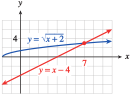
\includegraphics[width=0.5\linewidth]{images/fig-radical-equation}
\caption{\label{fig-radical-equation}}
\end{figure}
\par
The apparent solution \(2\) is extraneous. The only solution to the original equation is \(7\). We can verify the solution by graphing the equations%
\begin{equation*}
y_1=\sqrt{x+2} ~~~\text{ and }~~~ y_2=x-4
\end{equation*}
as shown in \hyperref[fig-radical-equation]{Figure~\ref{fig-radical-equation}}. The graphs intersect in only one point, \((7, 3)\), so there is only one solution, \(x=7\).%
\end{example}
\begin{warning}[]\label{warning-16}
When we square both sides of an equation, it is \emph{not} correct to square each term of the equation separately. Thus, in \hyperref[example-radical-equationS]{Example~\ref{example-radical-equationS}}, the original equation is not equivalent to%
\begin{equation*}
(\sqrt{x+2})^2+4^2=x^2 
\end{equation*}
This is because \((a + b)^2 \ne a^2 + b^2\). Instead, we must square the \emph{entire} left side of the equation as a binomial, like this,%
\begin{equation*}
(\sqrt{x+2}+4)^2=x^2 
\end{equation*}
or we may proceed as shown in \hyperref[example-radical-equationS]{Example~\ref{example-radical-equationS}}.%
\end{warning}
\typeout{************************************************}
\typeout{Subsection A.10.8 Equations with More than One Radical}
\typeout{************************************************}
\subsection[{Equations with More than One Radical}]{Equations with More than One Radical}\label{subsection-50}
Sometimes it is necessary to square both sides of an equation more than once in order to eliminate all the radicals.%
\begin{example}[]\label{example-79}
Solve \(\sqrt{x-7}+\sqrt{x}=7 \).%
\par\medskip\noindent%
\textbf{Solution.}\quad First, isolate the more complicated radical on one side of the equation. (This will make it easier to square both sides.) We will subtract \(\sqrt{x} \) from both sides.%
\begin{equation*}
\sqrt{x-7}=7-\sqrt{x} 
\end{equation*}
Now square each side to remove one radical. Be careful when squaring the binomial \(7-\sqrt{x} \).%
\begin{align*}
(\sqrt{x-7})^\alert{2}\amp =(7-\sqrt{x})^\alert{2}
\\
x-7\amp = 49-14\sqrt{x}+x
\end{align*}
Collect like terms, and isolate the radical on one side of the equation.%
\begin{align*}
−56 \amp = −14\sqrt{x}\amp\amp\text{Divide both sides by }−14.
\\
4 \amp = \sqrt{x}
\end{align*}
Now square again to obtain%
\begin{align*}
(4)^\alert{2} \amp = (\sqrt{x})^\alert{2}
\\
16 \amp = x
\end{align*}
\leavevmode%
\begin{description}
\item[{Check}]\hypertarget{li-361}{}Does \(\sqrt{\alert{16}-7}+\sqrt{\alert{16}}=7\)? \(\hphantom{blank}\text{Yes. The solution is } 16\).%
\end{description}
%
\end{example}
\typeout{************************************************}
\typeout{Section A.11 Facts from Geometry}
\typeout{************************************************}
\section[{Facts from Geometry}]{Facts from Geometry}\label{appendix-Facts-from-Geometry}
In this section, we review some information you will need from geometry. You are already familiar with the formulas for the area and perimeter of common geometric figures; you can find these formulas in the reference section at the front of the book.%
\typeout{************************************************}
\typeout{Subsection A.11.1 Right Triangles and the Pythagorean Theorem}
\typeout{************************************************}
\subsection[{Right Triangles and the Pythagorean Theorem}]{Right Triangles and the Pythagorean Theorem}\label{subsection-51}
A \terminology{right triangle} is a triangle in which one of the angles is a right angle, or \(90\degree\). Because the sum of the three angles in any triangle is \(180\degree\), this means that the other two angles in a right triangle must have a sum of \(180\degree-90\degree\), or \(90\degree\). For instance, if we know that one of the angles in a right triangle is \(37\degree\), then the remaining angle must be \(90\degree-37\degree\), or \(53\degree\), as shown in \hyperref[fig-right-triangle]{\ref{fig-right-triangle}}. \leavevmode%
\begin{figure}
\centering

\includegraphics[width=0.35\linewidth]{images/fig-right-triangle}
\caption{\label{fig-right-triangle}}
\end{figure}
%
\begin{example}[]\label{example-80}
In a right triangle, the medium-sized angle is \(15\degree\) less than twice the smallest angle. Find the sizes of the three angles in \hyperref[fig-right-triangle2]{\ref{fig-right-triangle2}}. \leavevmode%
\begin{figure}
\centering
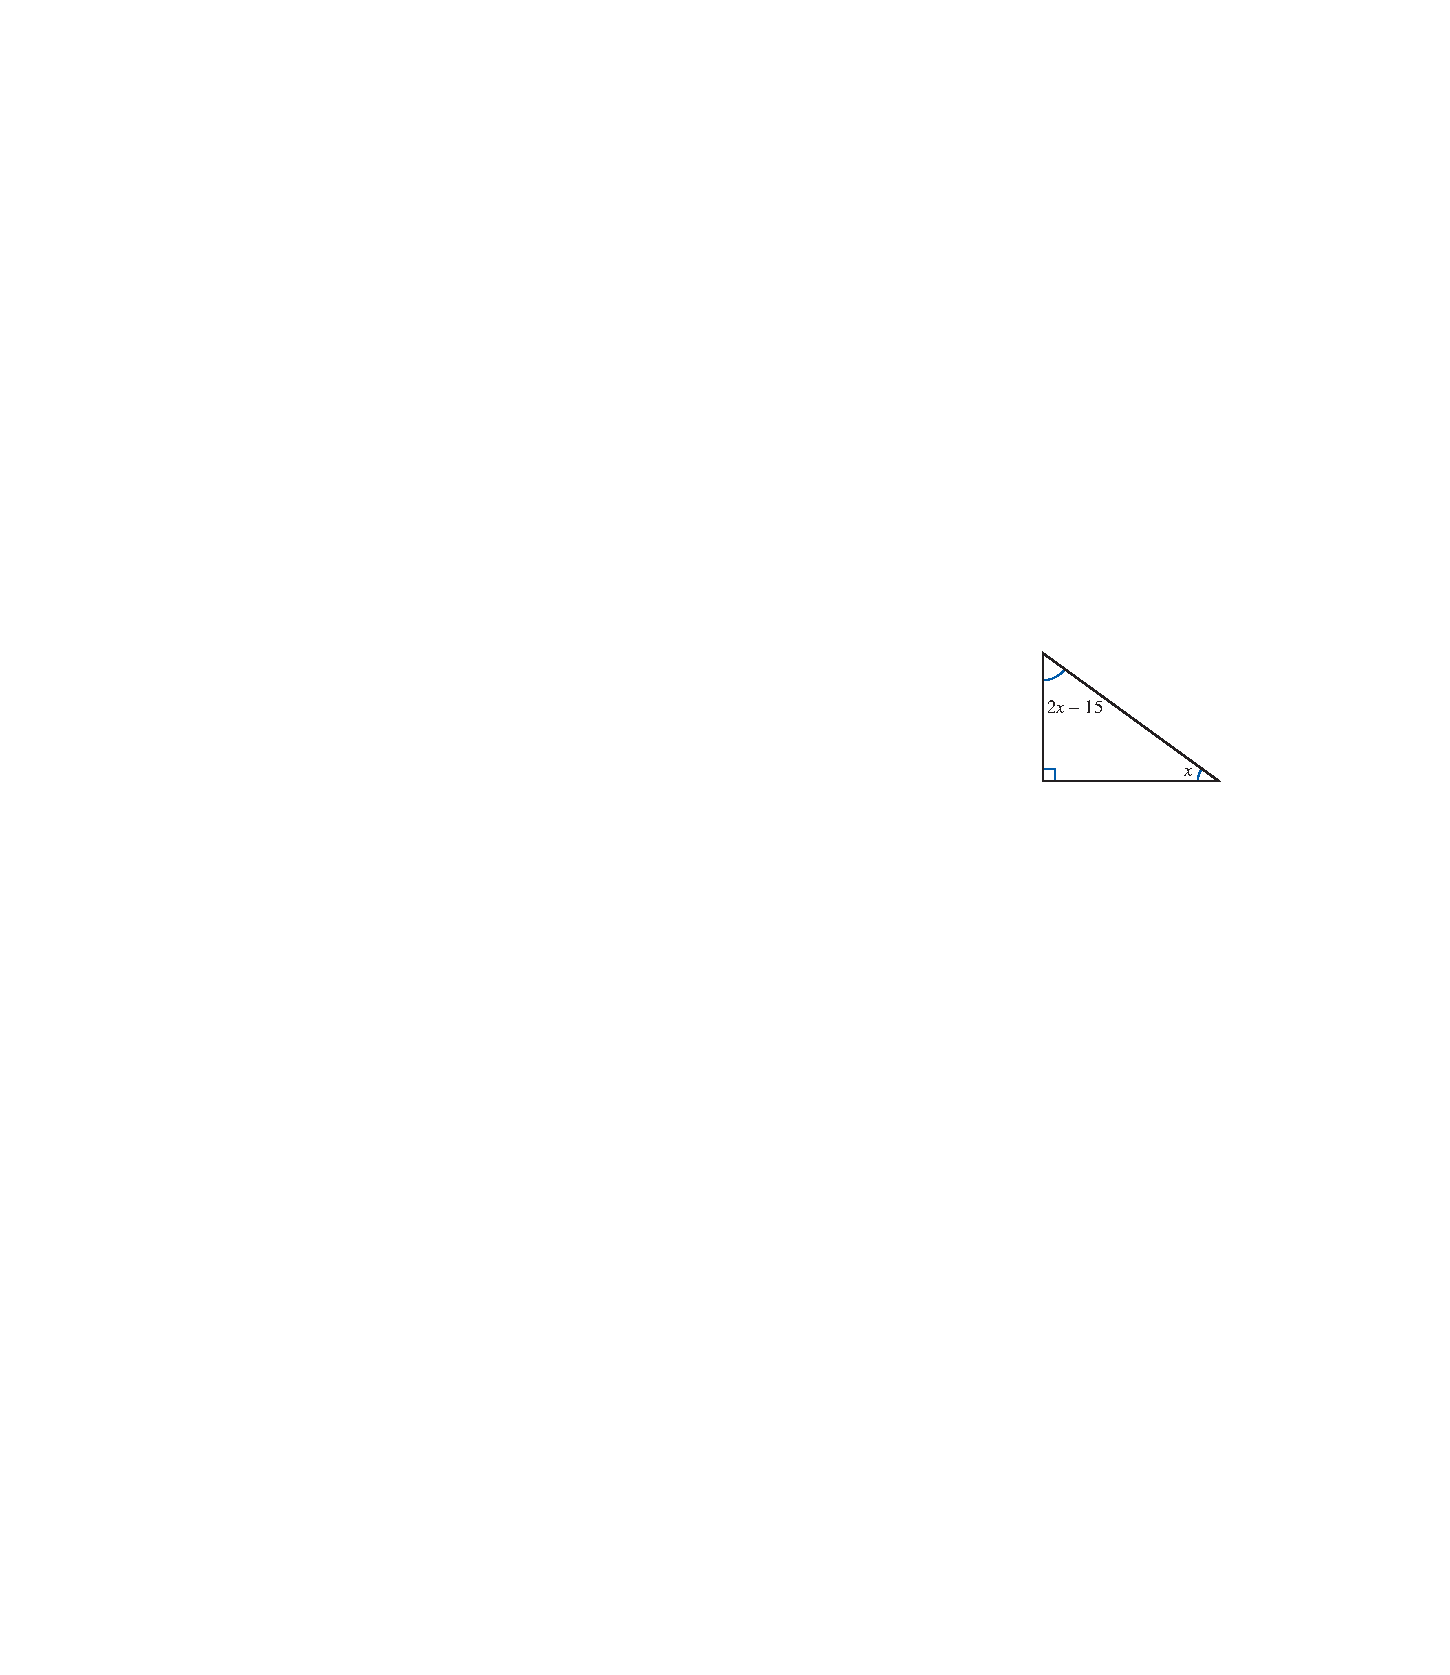
\includegraphics[width=0.3\linewidth]{images/fig-right-triangle2}
\caption{\label{fig-right-triangle2}}
\end{figure}
%
\par\medskip\noindent%
\textbf{Solution.}\quad \leavevmode%
\begin{description}
\item[{Step 1}]\hypertarget{li-362}{}Let \(x\) stand for the size of the smallest angle. Then the medium-sized angle must be \(2x-15\).%
\item[{Step 2}]\hypertarget{li-363}{}Because the right angle is the largest angle, the sum of the smallest and medium-sized angles must be the remaining \(90\degree\). Thus,%
\begin{equation*}
x + (2x − 15) = 90
\end{equation*}
%
\item[{Step 3}]\hypertarget{li-364}{}Solve the equation. Begin by simplifying the left side.%
\begin{align*}
3x − 15 \amp = 90\amp\amp\text{Add 15 to both sides.} \\
3x \amp = 105\amp\amp\text{Divide both sides by 3.}\\
x \amp = 35
\end{align*}
%
\item[{Step 4}]\hypertarget{li-365}{}The smallest angle is \(35\degree\), and the medium-sized angle is \(2(35\degree) −15\degree\), or \(55\degree\).%
\end{description}
%
\end{example}
\par
In a right triangle (see \hyperref[fig-right-triangle3]{Figure~\ref{fig-right-triangle3}}), the longest side is opposite the right angle and is called the \terminology{hypotenuse}. Ordinarily, even if we know the lengths of two sides of a triangle, it is not easy to find the length of the third side (to solve this problem we need trigonometry), but for the special case of a right triangle, there is an equation that relates the lengths of the three sides. This property of right triangles was known to many ancient cultures, and we know it today by the name of a Greek mathematician, Pythagoras, who provided a proof of the result. \leavevmode%
\begin{figure}
\centering
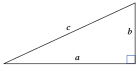
\includegraphics[width=0.4\linewidth]{images/fig-right-triangle3}
\caption{\label{fig-right-triangle3}}
\end{figure}
%
\begin{assemblage}{Pythagorean Theorem}\label{assemblage-34}
In a right triangle, if \(c\) stands for the length of the hypotenuse and \(a\) and \(b\) stand for the lengths of the two sides, then%
\begin{equation*}
a^2 + b^2 = c^2
\end{equation*}
%
\end{assemblage}
\begin{example}[]\label{example-81}
The hypotenuse of a right triangle is \(15\) feet long. The third side is twice the length of the shortest side. Find the lengths of the other 2 sides.%
\par\medskip\noindent%
\textbf{Solution.}\quad \leavevmode%
\begin{description}
\item[{Step 1}]\hypertarget{li-366}{}Let \(x\) represent the length of the shortest side, so that the third side has length \(2x\). (See \hyperref[fig-right-triangle4]{Figure~\ref{fig-right-triangle4}}.) \leavevmode%
\begin{figure}
\centering
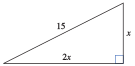
\includegraphics[width=0.6\linewidth]{images/fig-right-triangle4}
\caption{\label{fig-right-triangle4}}
\end{figure}
%
\item[{Step 2}]\hypertarget{li-367}{}Substituting these expressions into the Pythagorean theorem, we find%
\begin{equation*}
x^2+(2x)^2=15^2
\end{equation*}
%
\item[{Step 3}]\hypertarget{li-368}{}This is a quadratic equation with no linear term, so we simplify and then isolate \(x^2\).%
\begin{align*}
x^2+4x^2\amp =225\amp\amp\text{Combine like terms.} \\
5x^2\amp = 225\amp\amp\text{Divide both sides by 5.} \\
x^2\amp = 45
\end{align*}
Taking square roots of both sides yields%
\begin{equation*}
x=\pm\sqrt{45}\approx\pm 6.708203932 
\end{equation*}
%
\item[{Step 4}]\hypertarget{li-369}{}Because a length must be a positive number, the shortest side has length approximately \(6.71\) feet, and the third side has length \(2 (6.71)\), or approximately \(13.42\) feet.%
\end{description}
%
\end{example}
\typeout{************************************************}
\typeout{Subsection A.11.2 Isosceles and Equilateral Triangles}
\typeout{************************************************}
\subsection[{Isosceles and Equilateral Triangles}]{Isosceles and Equilateral Triangles}\label{subsection-52}
Recall also that an \terminology{isosceles} triangle is one that has at least two sides of equal length. In an isosceles triangle, the angles opposite the equal sides, called the \terminology{base} angles, are equal in measure, as shown in \hyperref[fig-isosceles-and-equilateral]{Figure~\ref{fig-isosceles-and-equilateral}}a. In an equilateral triangle (\hyperref[fig-isosceles-and-equilateral]{Figure~\ref{fig-isosceles-and-equilateral}}b), all three sides have equal length, and all three angles have equal measure. \leavevmode%
\begin{figure}
\centering
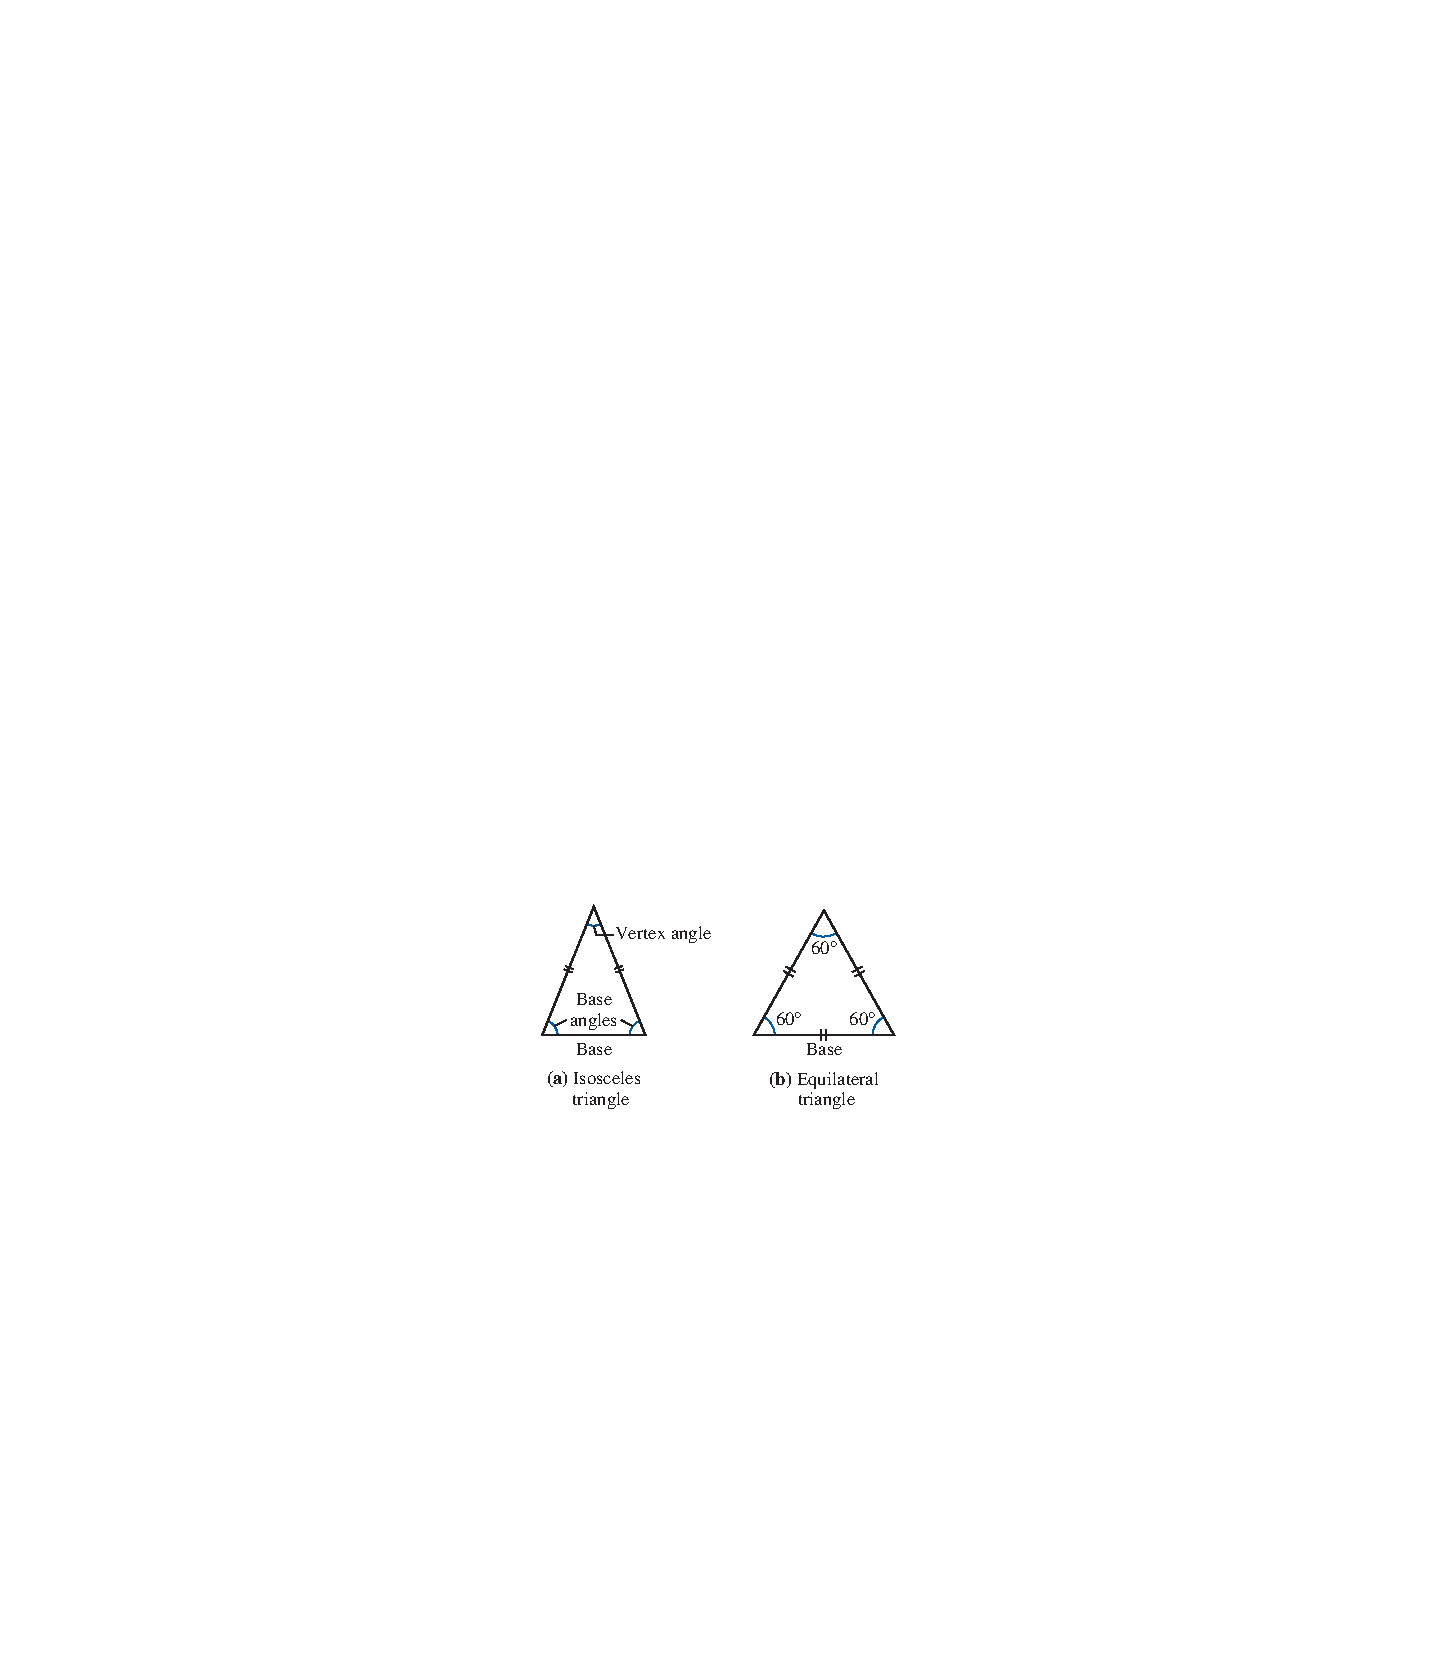
\includegraphics[width=0.55\linewidth]{images/fig-isosceles-and-equilateral}
\caption{\label{fig-isosceles-and-equilateral}}
\end{figure}
%
\typeout{************************************************}
\typeout{Subsection A.11.3 The Triangle Inequality}
\typeout{************************************************}
\subsection[{The Triangle Inequality}]{The Triangle Inequality}\label{subsection-53}
The longest side in a triangle is always opposite the largest angle, and the shortest side is opposite the smallest angle. It is also true that the sum of the lengths of any two sides of a triangle must be greater than the third side, or else the two sides will not meet to form a triangle! This fact is called the \terminology{triangle inequality}.%
\par
In \hyperref[fig-oblique-triangle]{Figure~\ref{fig-oblique-triangle}}, we must have that%
\begin{equation*}
p + q \gt r
\end{equation*}
where \(p\), \(q\), and \(r\) are the lengths of the sides of the triangle. \leavevmode%
\begin{figure}
\centering

\includegraphics[width=0.35\linewidth]{images/fig-oblique-triangle}
\caption{\label{fig-oblique-triangle}}
\end{figure}
%
\par
Now we can use the triangle inequality to discover information about the sides of a triangle.%
\begin{example}[]\label{example-82}
Two sides of a triangle have lengths \(7\) inches and \(10\) inches. What can you say about the length of the third side (see \hyperref[fig-oblique-triangle2]{Figure~\ref{fig-oblique-triangle2}})? \leavevmode%
\begin{figure}
\centering
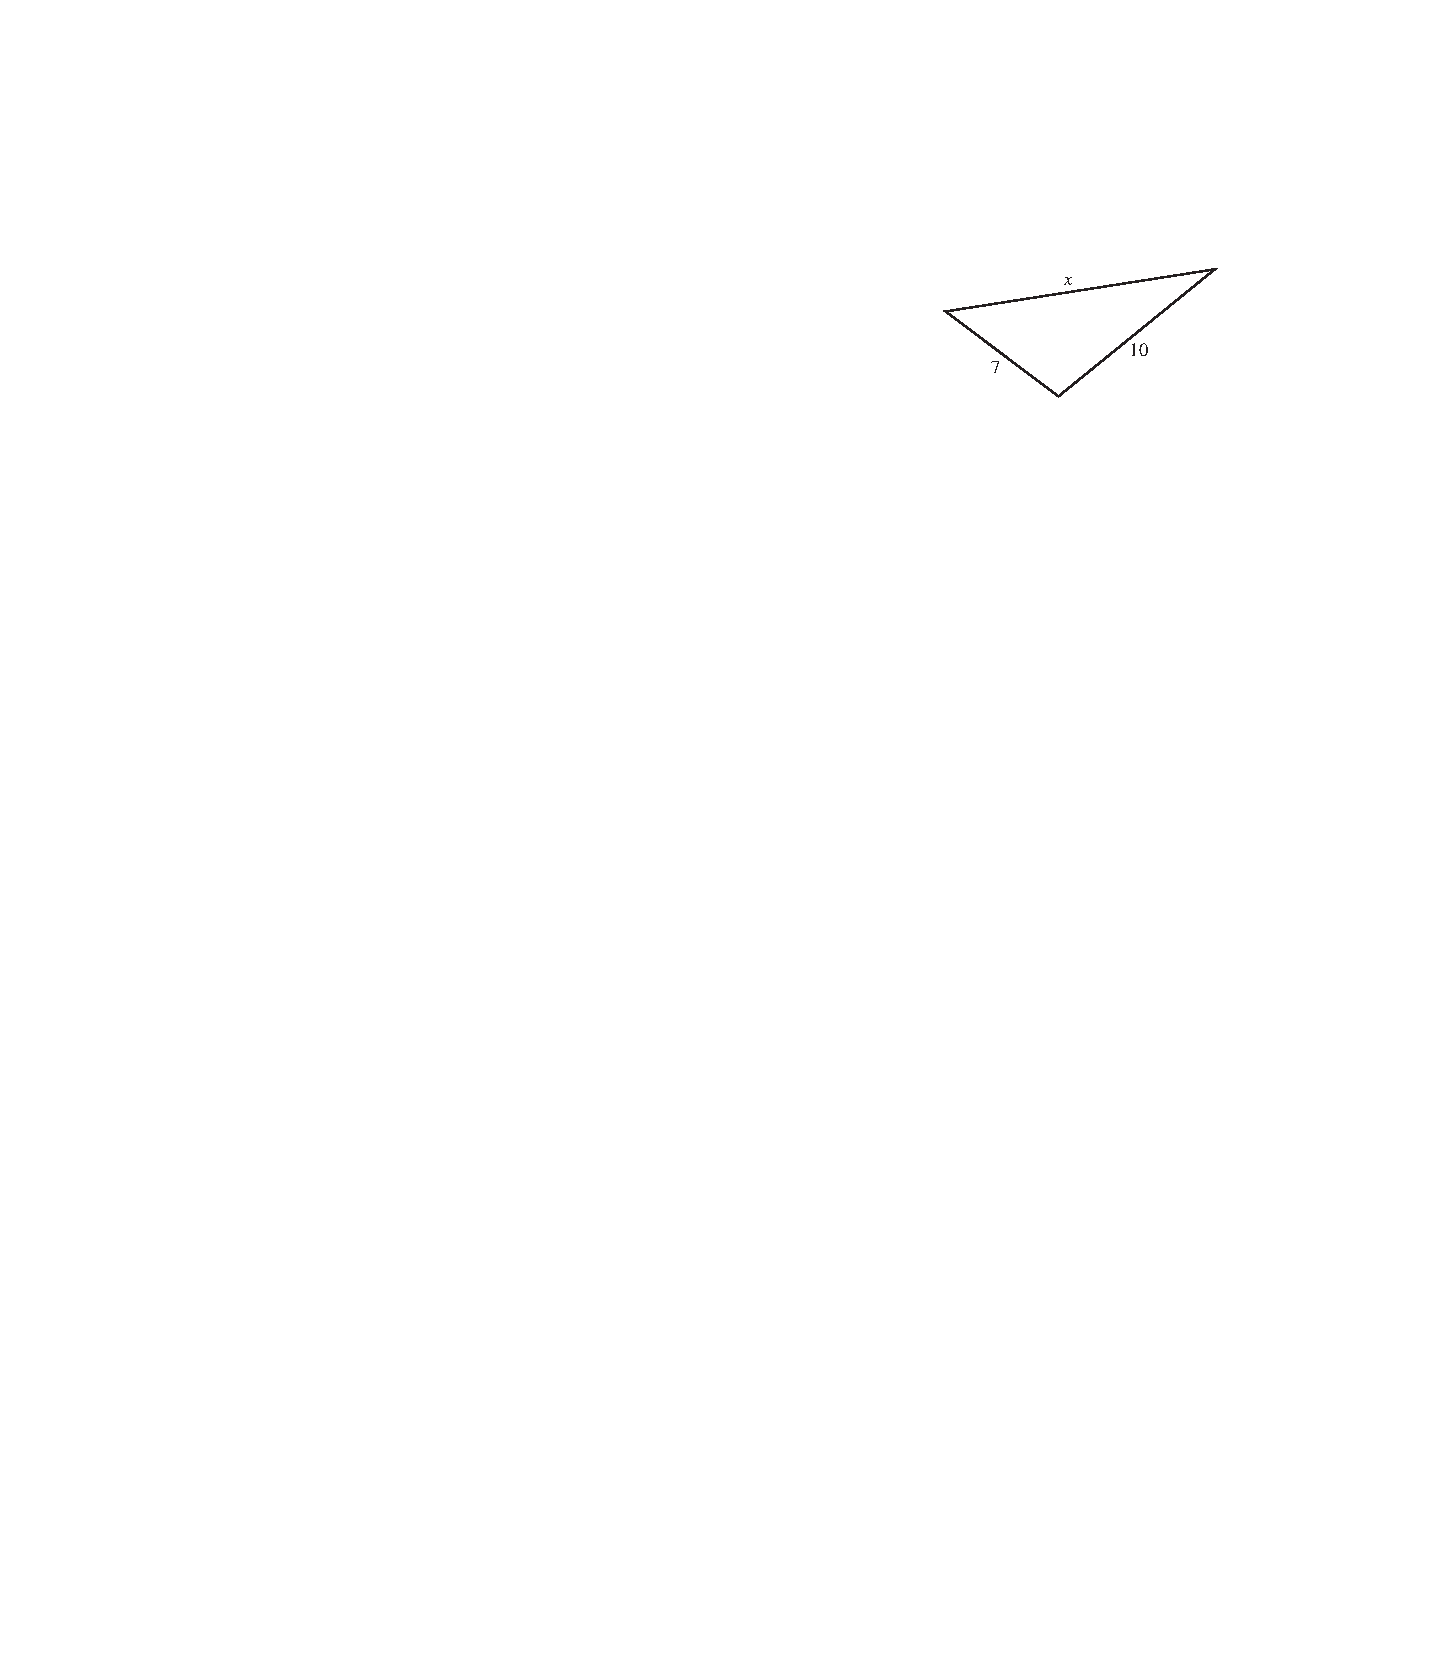
\includegraphics[width=0.5\linewidth]{images/fig-oblique-triangle2}
\caption{\label{fig-oblique-triangle2}}
\end{figure}
%
\par\medskip\noindent%
\textbf{Solution.}\quad Let \(x\) represent the length of the third side of the triangle. By the triangle inequality, we must have that%
\begin{equation*}
x \lt 7 + 10, ~~~\text{ or }~~~ x \ly 17
\end{equation*}
Looking at another pair of sides, we must also have that%
\begin{equation*}
10 \lt x + 7, ~~~\text{ or }~~~  x \gt 3
\end{equation*}
Thus the third side must be greater than \(3\) inches but less than \(17\) inches long.%
\end{example}
\typeout{************************************************}
\typeout{Subsection A.11.4 Similar Triangles}
\typeout{************************************************}
\subsection[{Similar Triangles}]{Similar Triangles}\label{subsection-54}
Two triangles are said to be \terminology{similar} if their corresponding angles are equal. This means that the two triangles will have the same shape but not necessarily the same size. One of the triangles will be an enlargement or a reduction of the other; so their corresponding sides are proportional. In other words, for similar triangles, the ratios of the corresponding sides are equal (see \hyperref[fig-similar-triangles]{Figure~\ref{fig-similar-triangles}}). \leavevmode%
\begin{figure}
\centering
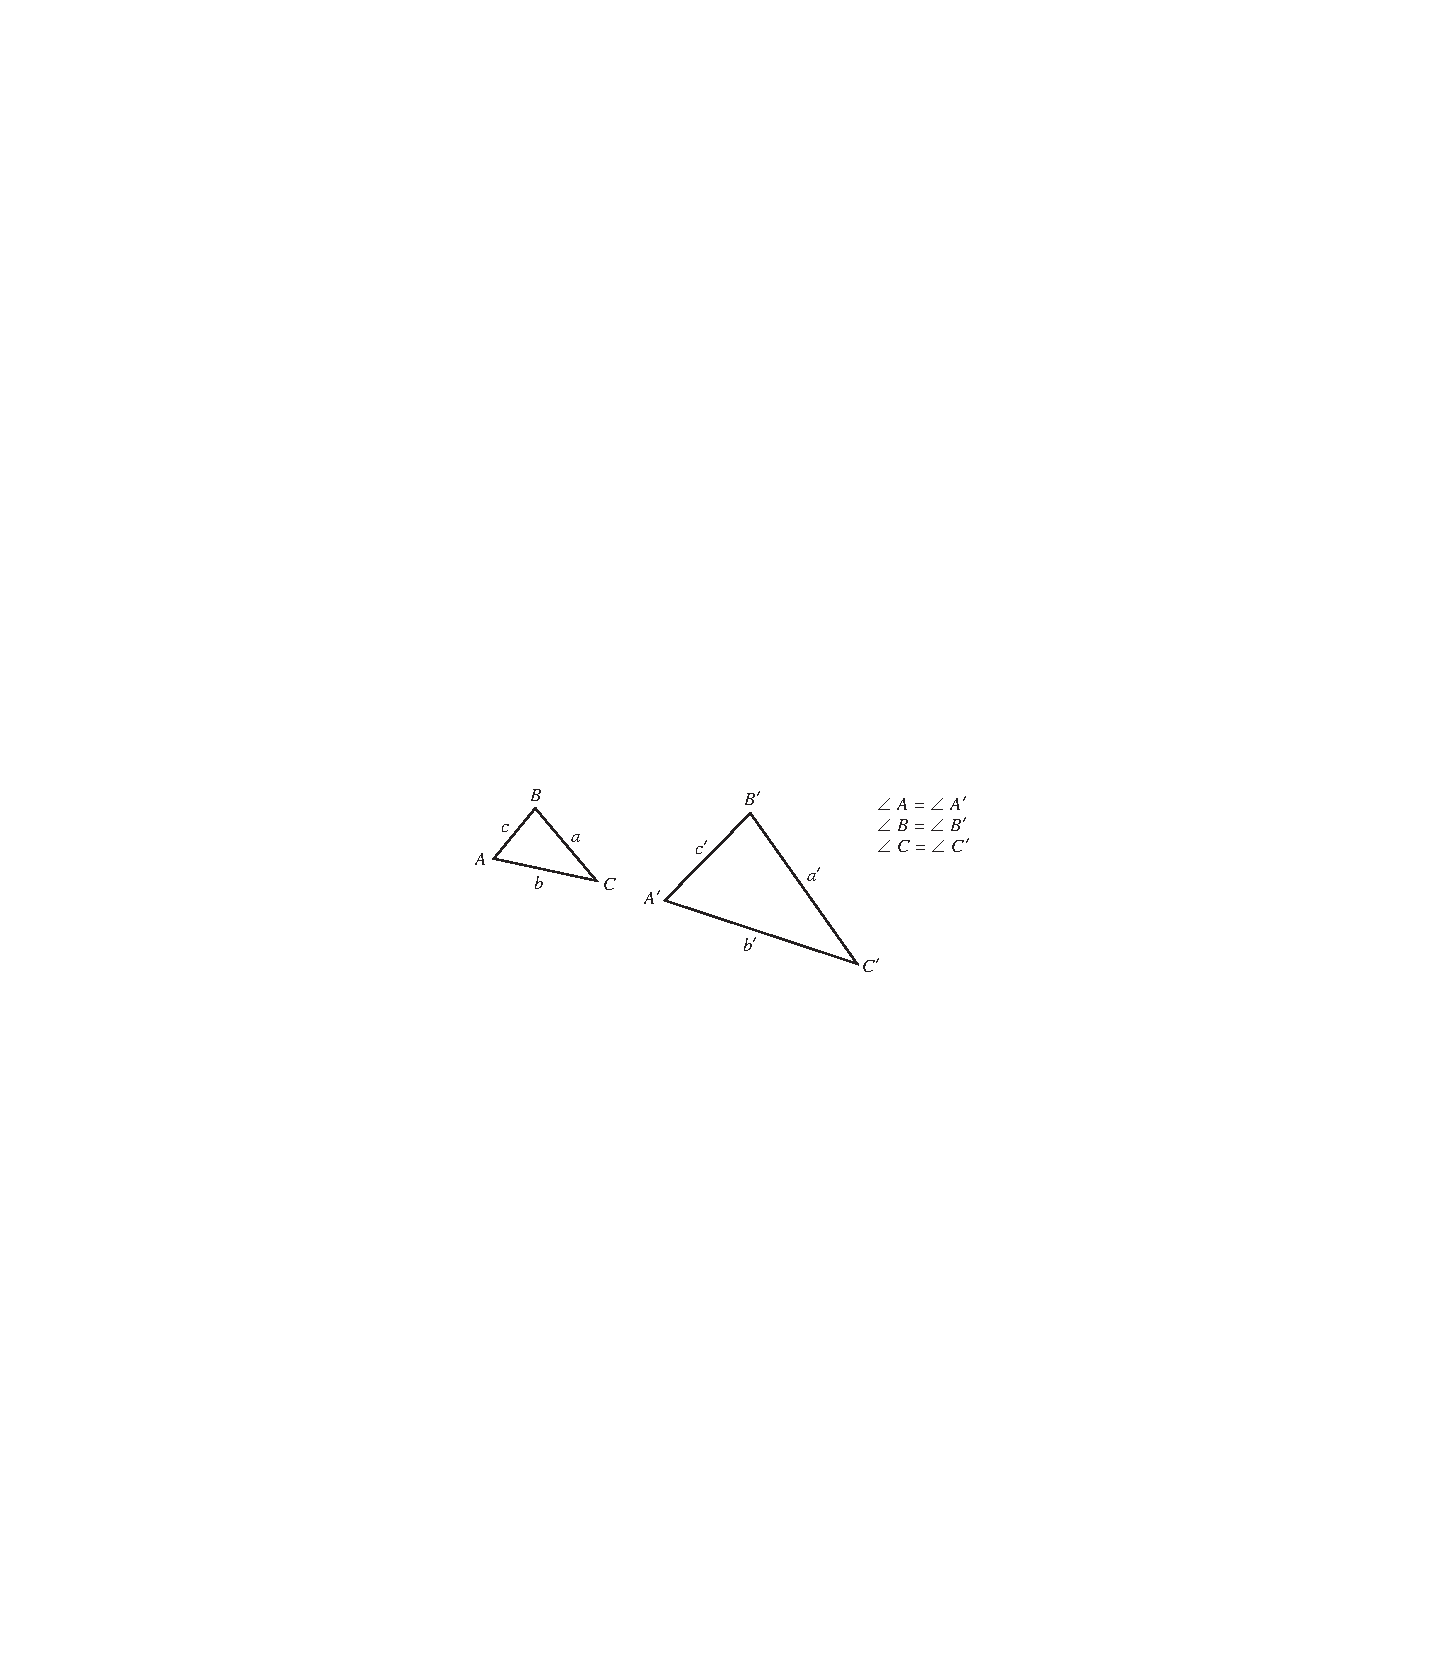
\includegraphics[width=0.7\linewidth]{images/fig-similar-triangles}
\caption{\label{fig-similar-triangles}}
\end{figure}
%
\par
If any two pairs of corresponding angles of two triangles are equal, then the third pair must also be equal, because in both triangles the sum of the angles is \(180\degree\). Thus, to show that two triangles are similar, we need only show that two pairs of angles are equal.%
\begin{example}[]\label{example-83}
The roof of an A-frame ski chalet forms an isosceles triangle with the floor as the base (see \hyperref[fig-A-frame-roof]{Figure~\ref{fig-A-frame-roof}}). The floor of the chalet is \(24\) feet wide, and the ceiling is \(20\) feet tall at the center. If a loft is built at a height of \(8\) feet from the floor, how wide will the loft be?%
% group protects changes to lengths, releases boxes (?)
{% begin: group for a single side-by-side
% set panel max height to practical minimum, created in preamble
\setlength{\panelmax}{0pt}
\newsavebox{\panelboxAXimage}
\savebox{\panelboxAXimage}{%
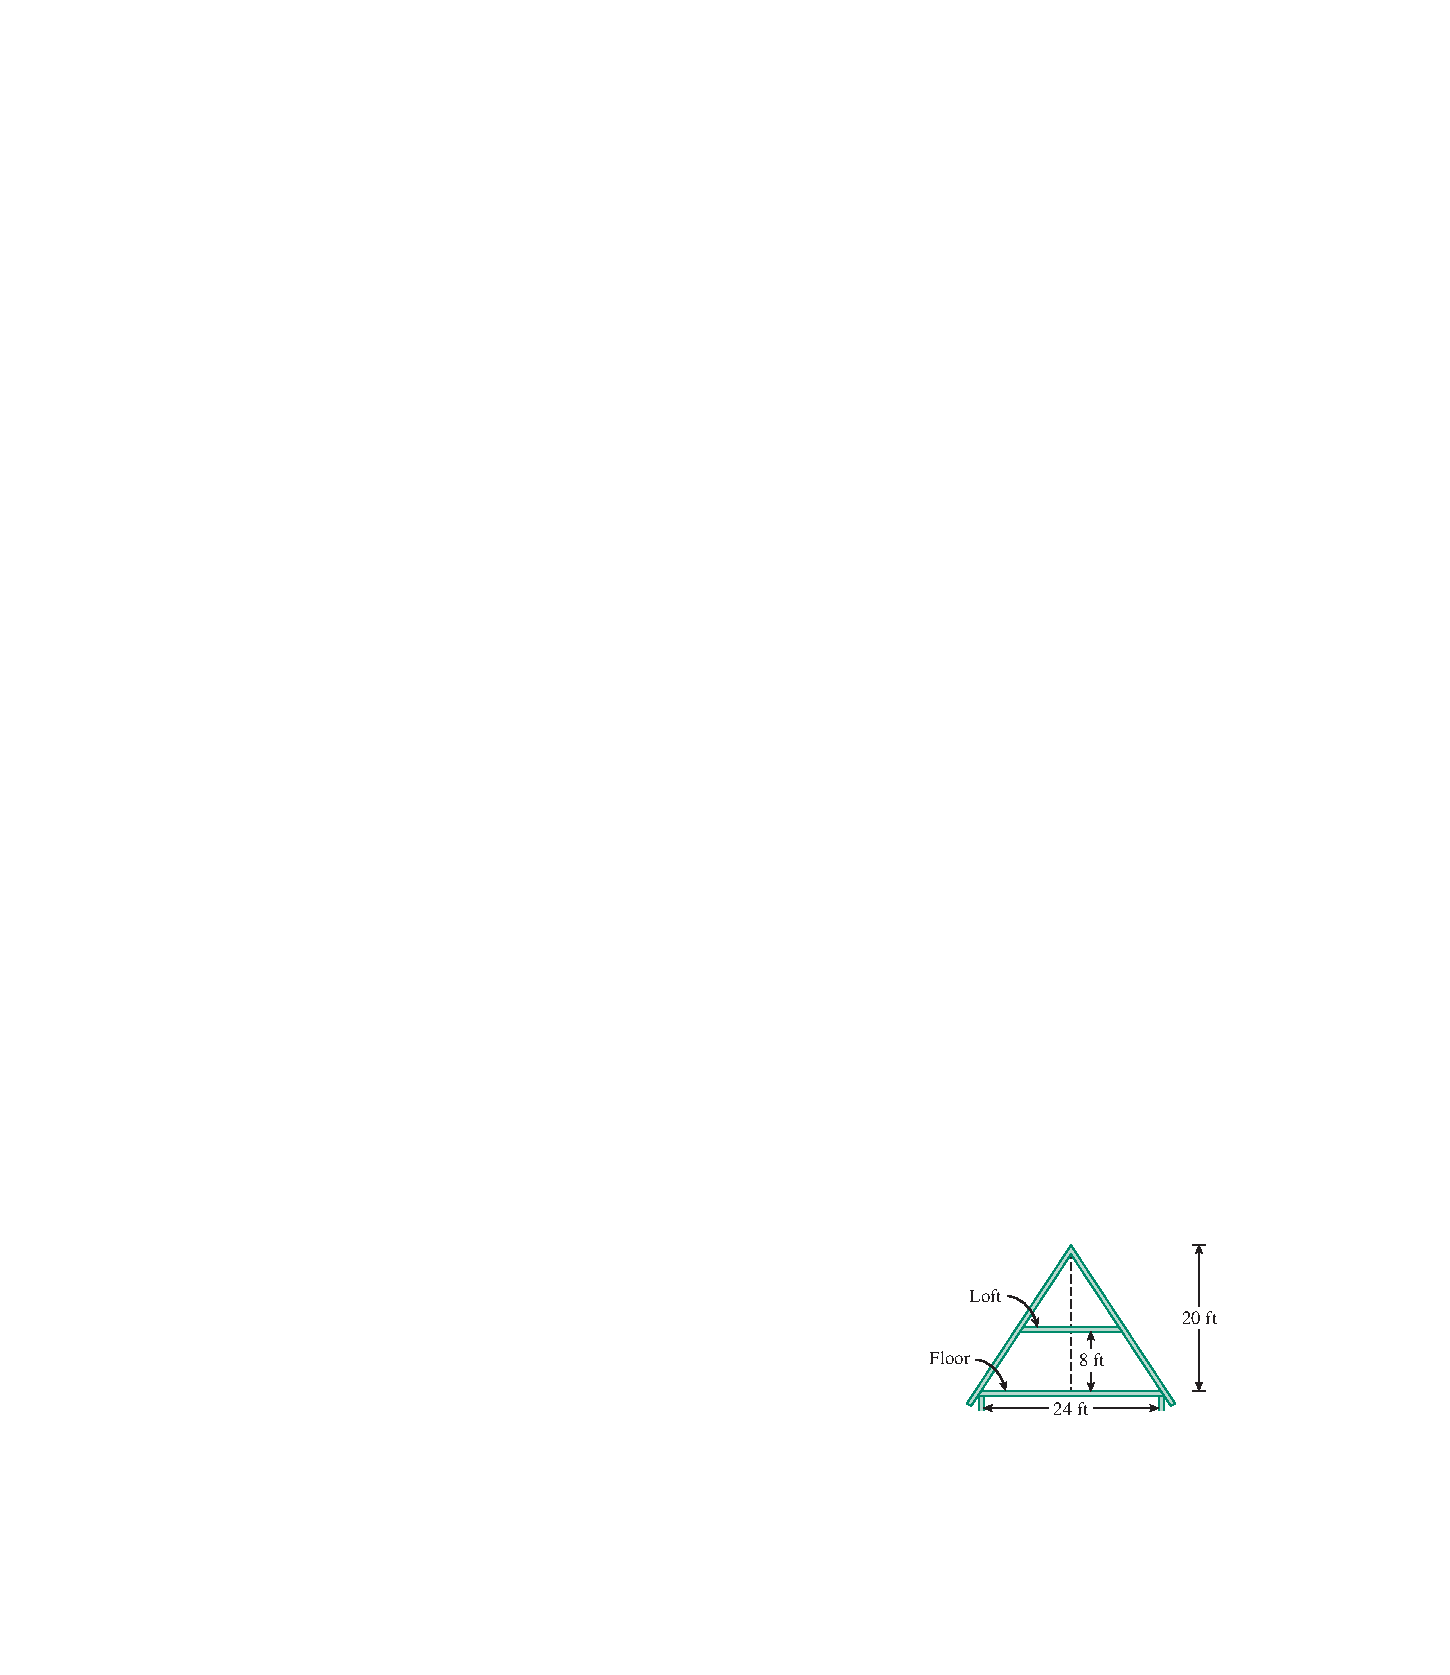
\includegraphics[width=0.45\linewidth]{images/fig-A-frame-roof}
}
\newlength{\phAXimage}\setlength{\phAXimage}{\ht\panelboxAXimage+\dp\panelboxAXimage}
\settototalheight{\phAXimage}{\usebox{\panelboxAXimage}}
\setlength{\panelmax}{\maxof{\panelmax}{\phAXimage}}
\newsavebox{\panelboxAYimage}
\savebox{\panelboxAYimage}{%
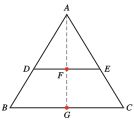
\includegraphics[width=0.4\linewidth]{images/fig-A-frame-roof2}
}
\newlength{\phAYimage}\setlength{\phAYimage}{\ht\panelboxAYimage+\dp\panelboxAYimage}
\settototalheight{\phAYimage}{\usebox{\panelboxAYimage}}
\setlength{\panelmax}{\maxof{\panelmax}{\phAYimage}}
\leavevmode%
% begin: side-by-side as figure/tabular
% \tabcolsep change local to group
\setlength{\tabcolsep}{0.0375\textwidth}
% @{} suppress \tabcolsep at extremes, so margins behave as intended
\begin{figure}
\hspace*{0.0375\textwidth}%
\begin{tabular}{@{}*{2}{c}@{}}
\begin{minipage}[c][\panelmax][t]{0.45\textwidth}\usebox{\panelboxAXimage}\end{minipage}&
\begin{minipage}[c][\panelmax][t]{0.4\textwidth}\usebox{\panelboxAYimage}\end{minipage}\tabularnewline
\parbox[t]{0.45\textwidth}{\captionof{figure}{\label{fig-A-frame-roof}}
}&
\parbox[t]{0.4\textwidth}{\captionof{figure}{\label{fig-A-frame-roof2}}
}\end{tabular}
\end{figure}
% end: side-by-side as tabular/figure
}% end: group for a single side-by-side
\par\medskip\noindent%
\textbf{Solution.}\quad From \hyperref[fig-A-frame-roof2]{Figure~\ref{fig-A-frame-roof2}}, we can show that \(\Delta ABC\) is similar to \(\Delta ADE\). Both triangles include \(\angle A\), and because \(\overline{DE}\) is parallel to \(\overline{BC} \), \(\angle ADE\) is equal to \(\angle ABC\). Thus, the triangles have two pairs of equal angles and are therefore similar triangles. \leavevmode%
\begin{description}
\item[{Step 1}]\hypertarget{li-370}{}Let \(w\) stand for the width of the loft.%
\item[{Step 2}]\hypertarget{li-371}{}First note that if \(FG = 8\), then \(AF = 12\). Because \(\Delta ABC\) is similar to \(\Delta ADE\), the ratios of their corresponding sides (or corresponding altitudes) are equal. In particular,%
\begin{equation*}
\frac{w}{24}=\frac{12}{20}  
\end{equation*}
%
\item[{Step 3}]\hypertarget{li-372}{}Solve the proportion for \(w\). Begin by cross-multiplying.%
\begin{align*}
20w \amp = (12)(24)\amp\amp\text{Apply the fundamental principle.}
\\
w \amp = \frac{288}{20}= 14.4\amp\amp\text{Divide by 20.}
\end{align*}
%
\item[{Step 4}]\hypertarget{li-373}{}The floor of the loft will be \(14.4\) feet wide.%
\end{description}
%
\end{example}
\typeout{************************************************}
\typeout{Subsection A.11.5 Volume and Surface Area}
\typeout{************************************************}
\subsection[{Volume and Surface Area}]{Volume and Surface Area}\label{subsection-55}
\leavevmode%
\begin{figure}
\centering
\includegraphics[width=0.4\linewidth]{images/fig-box2}
\caption{\label{fig-box2}}
\end{figure}
 The \terminology{volume} of a three-dimensional object measures its capacity, or how much space it encloses. Volume is measured in cubic units, such as cubic inches or cubic meters. The volume of a rectangular prism, or box, is given by the product of its length, width, and height. For example, the volume of the box of length \(4\) inches, width \(3\) inches, and height \(2\) inches shown in \hyperref[fig-box2]{Figure~\ref{fig-box2}} is%
\begin{equation*}
V = lwh = 4(3)(2) = 24 \text{ cubic inches}
\end{equation*}
%
\par
Formulas for the volumes of other common objects can be found inside the front cover of the book.%
\begin{example}[]\label{example-84}
A cylindrical can must have a height of \(6\) inches, but it can have any reasonable radius. \leavevmode%
\begin{enumerate}[label=*\alph**]
\item\hypertarget{li-374}{}Write an algebraic expression for the volume of the can in terms of its radius.%
\item\hypertarget{li-375}{}If the volume of the can should be approximately \(170\) cubic inches, what should its radius be?%
\end{enumerate}
%
\par\medskip\noindent%
\textbf{Solution.}\quad \leavevmode%
\begin{enumerate}[label=*\alph**]
\item\hypertarget{li-376}{}The formula for the volume of a right circular cylinder is \(V = \pi r^2h\). If the height of the cylinder is \(6\) inches, then \(V = \pi r^2 (6)\), or \(V = 6\pi r^2\). (See \hyperref[fig-cylinder]{Figure~\ref{fig-cylinder}}.) \leavevmode%
\begin{figure}
\centering
\includegraphics[width=0.3\linewidth]{images/fig-cylinder}
\caption{\label{fig-cylinder}}
\end{figure}
%
\item\hypertarget{li-377}{}Substitute \(170\) for \(V\) and solve for \(r\).%
\begin{align*}
170 \amp = 6\pi r^2\amp\amp\text{Divide both sides by }6\pi.
\\
r^2 \amp = \frac{170}{6\pi} \amp\amp\text{Take square roots.}
\\
r \amp = \sqrt{\frac{170}{6\pi}}\approx 3.00312
\end{align*}
Thus, the radius of the can should be approximately \(3\) inches. A calculator keying sequence for the expression above is%
\begin{equation*}
\boxed{\sqrt{~}} \,\boxed{(} \, 170 \, \boxed{\div} \, \boxed{(} \, 6 \, \boxed{\pi} \, \boxed{)}  \, \boxed{)} \, \boxed{\text{ENTER}} 
\end{equation*}
%
\end{enumerate}
%
\end{example}
\par
The \terminology{surface area} of a solid object is the sum of the areas of all the exterior faces of the object. It measures the amount of paper that would be needed to cover the object entirely. Since it is an area, it is measured in square units.%
\begin{example}[]\label{example-85}
Write a formula for the surface area of a closed box in terms of its length, width, and height. (See \hyperref[fig-box2a]{Figure~\ref{fig-box2a}}.) \leavevmode%
\begin{figure}
\centering
\includegraphics[width=0.4\linewidth]{images/fig-box2}
\caption{\label{fig-box2a}}
\end{figure}
%
\par\medskip\noindent%
\textbf{Solution.}\quad The box has six sides; we must find the area of each side and add them. The top and bottom of the box each have area \(lw\), so together they contribute \(2lw\) to the surface area. The back and front of the box each have area \(lh\), so they contribute \(2lh\) to the surface area. Finally, the left and right sides of the box each have area \(wh\), so they add \(2wh\) to the surface area. Thus, the total surface area is%
\begin{equation*}
S = 2lw + 2lh + 2wh
\end{equation*}
%
\end{example}
\par
Formulas for the surface areas of other common solids can be found on the insert in the front of the book.%
\typeout{************************************************}
\typeout{Subsection A.11.6 The Distance Formula}
\typeout{************************************************}
\subsection[{The Distance Formula}]{The Distance Formula}\label{subsection-56}
By using the Pythagorean theorem, we can derive a formula for the distance between two points, \(P_1\) and \(P_2\), in terms of their coordinates. We first label a right triangle, as we did in the example above. Draw a horizontal line through \(P_1\) and a vertical line through \(P_2\). These lines meet at a point \(P_3\), as shown in \hyperref[fig-distance-formula]{Figure~\ref{fig-distance-formula}}. The \(x\)-coordinate of \(P_3\) is the same as the \(x\)-coordinate of \(P_2\), and the \(y\)-coordinate of \(P_3\) is the same as the \(y\)-coordinate of \(P_1\). Thus, the coordinates of \(P_3\) are \((x_2, y_1)\). \leavevmode%
\begin{figure}
\centering
\includegraphics[width=0.75\linewidth]{images/fig-distance-formula}
\caption{\label{fig-distance-formula}}
\end{figure}
%
\par
The distance between \(P_1\) and \(P_3\) is \(\abs{x_2-x_1}\) , and the distance between \(P_2\) and \(P_3\) is \(\abs{y_2-y_1} \). (See {$\langle\langle$Unresolved xref, reference "AbsoluteValue"; check spelling or use "provisional" attribute$\rangle\rangle$} to review distance and absolute value.) These two numbers are the lengths of the legs of the right triangle. The length of the hypotenuse is the distance between \(P_1\) and \(P_2\), which we will call \(d\). By the Pythagorean theorem,%
\begin{equation*}
d^2 = (x_2 − x_1)^2 + (y_2 − y_1)^2
\end{equation*}
Taking the (positive) square root of each side of this equation gives us the \terminology{distance formula}.%
\begin{assemblage}{Distance Formula}\label{assemblage-35}
The \terminology{distance} \(d\) between points \(P_1(x_1, y_1)\) and \(P_2(x_2, y_2)\) is%
\begin{equation*}
d=\sqrt{(x_2 − x_1)^2 + (y_2 − y_1)^2} 
\end{equation*}
%
\end{assemblage}
\begin{example}[]\label{example-distance-formula}
Find the distance between \((2, −1)\) and \((4, 3)\).%
\par\medskip\noindent%
\textbf{Solution.}\quad Substitute \((2, −1)\) for \((x_1, y_1)\) and substitute \((4, 3)\) for \((x_2, y_2)\) in the distance formula to obtain%
\begin{align*}
d\amp =\sqrt{(x_2 − x_1)^2 + (y_2 − y_1)^2}
\\
\amp =\sqrt{(4 − 2)^2 + \left[3 − (-1)\right]^2} 
\\
\amp = \sqrt{4+16}=\sqrt{20}\approx 4.47
\end{align*}
%
\end{example}
\par
In \hyperref[example-distance-formula]{Example~\ref{example-distance-formula}}, we obtain the same answer if we use \((4, 3)\) for \(P_1\) and use \((2,−1)\) for \(P_2\):%
\begin{align*}
d\amp =\sqrt{(2-4)^2 + \left[(-1)-3\right]^2} 
\\
\amp = \sqrt{4+16}=\sqrt{20}
\end{align*}
%
\typeout{************************************************}
\typeout{Subsection A.11.7 The Midpoint Formula}
\typeout{************************************************}
\subsection[{The Midpoint Formula}]{The Midpoint Formula}\label{subsection-57}
If we know the coordinates of two points, we can calculate the coordinates of the point halfway between them using the \terminology{midpoint} formula. Each coordinate of the midpoint is the average of the corresponding coordinates of the two points.%
\begin{assemblage}{Midpoint Formula}\label{assemblage-36}
The \terminology{midpoint} of the line segment joining the points \(P_1(x_1, y_1)\) and \(P_2(x_2, y_2)\) is the point \(M(\overline{x}, \overline{y})\), where%
\begin{equation*}
\overline{x} = \frac{x_1 + x_2}{2} ~~~\text{ and }~~~
\overline{y} = \frac{y_1 + y_2}{2}
\end{equation*}
%
\end{assemblage}
\begin{example}[]\label{example-87}
Find the midpoint of the line segment joining the points \((−2, 1)\) and \((4, 3)\).%
\par\medskip\noindent%
\textbf{Solution.}\quad Substitute \((−2, 1)\) for \((x_1, y_1)\) and \((4, 3)\) for \((x_2, y_2)\) in the midpoint formula to obtain%
\begin{align*}
\overline{x} \amp= \frac{x_1 + x_2}{2}=\frac{-2+4}{2}=1\amp\amp\text{and}
\\
\overline{y} \amp= \frac{y_1 + y_2}{2}=\frac{1+3}{2}=2
\end{align*}
The midpoint of the segment is the point \((\overline{x}, \overline{y}) = (1, 2)\).%
\end{example}
\typeout{************************************************}
\typeout{Subsection A.11.8 Circles}
\typeout{************************************************}
\subsection[{Circles}]{Circles}\label{subsection-58}
A \terminology{circle} is the set of all points in a plane that lie at a given distance, called the \terminology{radius}, from a fixed point called the \terminology{center}. We can use the distance formula to find an equation for a circle. First consider the circle in \hyperref[fig-circles]{Figure~\ref{fig-circles}}a, whose center is the origin, \((0, 0)\). \leavevmode%
\begin{figure}
\centering
\includegraphics[width=0.9\linewidth]{images/fig-circles}
\caption{\label{fig-circles}}
\end{figure}
%
\par
The distance from the origin to any point \(P(x, y)\) on the circle is \(r\). Therefore,%
\begin{equation*}
\sqrt{(x − 0)^2 + (y − 0)^2} = r 
\end{equation*}
Or, squaring both sides,%
\begin{equation*}
(x − 0)^2 + (y − 0)^2 = r^2
\end{equation*}
Thus, the equation for a circle of radius \(r\) centered at the origin is%
\begin{equation*}
x^2 + y^2 = r^2
\end{equation*}
%
\par
Now consider the circle in \hyperref[fig-circles]{Figure~\ref{fig-circles}}b, whose center is the point \((h, k)\). Every point \(P(x, y)\) on the circle lies a distance \(r\) from \((h, k)\), so the equation of the circle is given by the following formula.%
\begin{assemblage}{Standard Form for a Circle}\label{assemblage-37}
The equation for a \terminology{circle} of \terminology{radius} \(r\) centered at the point \((h, k)\) is%
\begin{equation*}
(x − h)^2 + (y − k)^2 = r^2
\end{equation*}
%
\end{assemblage}
\par
This equation is the \terminology{standard form} for a circle of radius \(r\) with center at \((h, k)\). It is easy to graph a circle if its equation is given in standard form.%
\begin{example}[]\label{example-88}
Graph the circles. \leavevmode%
\begin{enumerate}[label=*\alph**]
\item\hypertarget{li-378}{}\((x − 2)^2 + (y + 3)^2 = 16\)%
\item\hypertarget{li-379}{}\(x^2 + (y − 4)^2 = 7\)%
\end{enumerate}
%
\par\medskip\noindent%
\textbf{Solution.}\quad \leavevmode%
\begin{enumerate}[label=*\alph**]
\item\hypertarget{li-380}{}The graph of \((x − 2)^2 + (y + 3)^2 = 16\) is a circle with radius \(4\) and center at \((2, −3)\). To sketch the graph, first locate the center of the circle. (The center is not part of the graph of the circle.) From the center, move a distance of \(4\) units (the radius of the circle) in each of four directions: up, down, left, and right. This locates four points that lie on the circle: \((2, 1)\), \((2, −7)\), \((−2, −3)\), and \((6, −3)\). Sketch the circle through these four points. (See \hyperref[fig-circles2]{Figure~\ref{fig-circles2}}a.) \leavevmode%
\begin{figure}
\centering
\includegraphics[width=1\linewidth]{images/fig-circles2}
\caption{\label{fig-circles2}}
\end{figure}
%
\item\hypertarget{li-381}{}The graph of \(x^2 + (y − 4)^2 = 7\) is a circle with radius \(\sqrt{7} \) and center at \((0, 4)\). From the center, move \(\sqrt{7} \), or approximately \(2.6\), units in each of the four coordinate directions to obtain the points \((0, 6.6)\), \((0, 1.4)\), \((−2.6, 4)\), and \((2.6, 4)\). Sketch the circle through these four points. (See \hyperref[fig-circles2]{Figure~\ref{fig-circles2}}b.)%
\end{enumerate}
%
\end{example}
\par
We can write an equation for any circle if we can find its center and radius.%
\begin{example}[]\label{example-89}
Find an equation for the circle whose diameter has endpoints \((7, 5)\) and \((1,−1)\).%
\par\medskip\noindent%
\textbf{Solution.}\quad The center of the circle is the midpoint of its diameter (see \hyperref[fig-circle-irrational-radius]{Figure~\ref{fig-circle-irrational-radius}}). Use the midpoint formula to find the center: \leavevmode%
\begin{figure}
\centering
\includegraphics[width=0.35\linewidth]{images/fig-circle-irrational-radius}
\caption{\label{fig-circle-irrational-radius}}
\end{figure}
%
\begin{gather*}
h = \overline{x} = \frac{7 + 1}{2}= 4
\\
k = \overline{y} = \frac{ 5 − 1}{2}= 2
\end{gather*}
Thus, the center is the point \((h, k) = (4, 2)\). The radius is the distance from the center to either of the endpoints of the diameter, say the point \((7, 5)\). Use the distance formula with the points \((7, 5)\) and \((4, 2)\) to find the radius.%
\begin{align*}
r\amp =\sqrt{(7 − 4)^2 + (5 − 2)^2}
\\
\amp = \sqrt{3^2 + 3^2}=\sqrt{18}
\end{align*}
Finally, substitute \(4\) for \(h\) and \(2\) for \(k\) (the coordinates of the center) and \(\sqrt{18} \) for \(4\) (the radius) into the standard form to obtain%
\begin{align*}
(x − h)^2 + (y − k)^2 \amp= r^2
\\
(x − 4)^2 + (y − 2)^2 \amp = 18
\end{align*}
%
\end{example}
\typeout{************************************************}
\typeout{Section A.12 The Real Number System}
\typeout{************************************************}
\section[{The Real Number System}]{The Real Number System}\label{appendix-The-Real-Number-System}
\typeout{************************************************}
\typeout{Subsection A.12.1 Subsets of the Real Numbers}
\typeout{************************************************}
\subsection[{Subsets of the Real Numbers}]{Subsets of the Real Numbers}\label{subsection-59}
The numbers associated with points on a number line are called the \terminology{real numbers}. The set of real numbers is denoted by \(\mathbb{R}\). You are already familiar with several types, or subsets, of real numbers: \leavevmode%
\begin{itemize}[label=\textbullet]
\item{}The set \(\mathbb{N} \) of \terminology{natural}\index{natural numbers}, or \terminology{counting numbers}, as its name suggests, consists of the numbers \(1, 2, 3, 4 , \ldots ,\) where "\(\ldots\)" indicates that the list continues without end.%
\item{}The set \(\mathbb{W} \) of \terminology{whole numbers} consists of the natural numbers and zero: \(0, 1, 2, 3 \ldots\).%
\item{}The set \(\mathbb{Z} \) of \terminology{integers} consists of the natural numbers, their negatives, and zero: \(\ldots , −3, −2, −1, 0, 1, 2, 3, \ldots\).%
\end{itemize}
 All of these numbers are subsets of the rational numbers.%
\typeout{************************************************}
\typeout{Subsection A.12.2 Rational Numbers}
\typeout{************************************************}
\subsection[{Rational Numbers}]{Rational Numbers}\label{subsection-60}
A number that can be expressed as the quotient of two integers \(\frac{a}{b} \) where \(b\ne 0\), is called a \terminology{rational number}. The integers are rational numbers, and so are common fractions. Some examples of rational numbers are \(5, −2, 0, \frac{2}{9} , \sqrt{16},\) and \(\frac{-4}{17} \). The set of rational numbers is denoted by \(\mathbb{Q} \).%
\par
Every rational number has a decimal form that either terminates or repeats a pattern of digits. For example,%
\begin{equation*}
\frac{3}{4}=3\div 4=0.75, ~\text{a }\textbf{terminating decimal}
\end{equation*}
and%
\begin{equation*}
\frac{2}{37}=9\div 37=0.243243243 \ldots
\end{equation*}
where the pattern of digits \(243\) is repeated endlessly. We use the \terminology{repeater bar} notation to write a repeating decimal fraction:%
\begin{equation*}
\frac{9}{37}= 0.\overline{243}
\end{equation*}
%
\typeout{************************************************}
\typeout{Subsection A.12.3 Irrational Numbers}
\typeout{************************************************}
\subsection[{Irrational Numbers}]{Irrational Numbers}\label{subsection-61}
Some real numbers \emph{cannot} be written in the form \(\frac{a}{b} \) , where \(a\) and \(b\) are integers. For example, the number \(\sqrt{2} \) is not equal to any common fraction. Such numbers are called \terminology{irrational numbers}. Examples of irrational numbers are \(\sqrt{15}, \pi, \) and \(-\sqrt[3]{7} \).%
\par
The decimal form of an irrational number never terminates, and its digits do not follow a repeating pattern, so it is impossible to write down an exact decimal equivalent for an irrational number. However, we can obtain decimal \emph{approximations} correct to any desired degree of accuracy by rounding off. A graphing calculator gives the decimal representation of \(\pi\) as \(3.141592654\). This is not the \emph{exact} value of \(\pi\), but for most calculations it is quite adequate.%
\par
Some \(n\)th roots are rational numbers and some are irrational numbers. For example,%
\begin{equation*}
\sqrt{49}. \sqrt[3]{\frac{27}{8}}, \text{ and } 81^{1/4}
\end{equation*}
are rational numbers because they are equal to \(7, \frac{3}{2},\) and \(3\), respectively. On the other hand,%
\begin{equation*}
\sqrt{5}, \sqrt[3]{54}, \text{ and } 7^{1/5} 
\end{equation*}
are irrational numbers. We can use a calculator to obtain decimal approximations for each of these numbers:%
\begin{equation*}
\sqrt{5}\approx 2.236, ~~~\sqrt[3]{54}\approx 3.826, ~~~\text{ and }~~~ 7^{1/5}\approx 1.476 
\end{equation*}
%
\par
The subsets of the real numbers are related as shown in \hyperref[fig-real-numbers]{Figure~\ref{fig-real-numbers}}. Every natural number is also a whole number, every whole number is an integer, every integer is a rational number, and every rational number is real. Also, every real number is either rational or irrational. \leavevmode%
\begin{figure}
\centering
\includegraphics[width=0.8\linewidth]{images/fig-real-numbers}
\caption{\label{fig-real-numbers}}
\end{figure}
%
\begin{example}[]\label{example-90}
\leavevmode%
\begin{enumerate}[label=*\alph**]
\item\hypertarget{li-385}{}\(2\) is a natural number, a whole number, an integer, a rational number, and a real number.%
\item\hypertarget{li-386}{}\(\sqrt{15}\) is an irrational number and a real number.%
\item\hypertarget{li-387}{}The number \(\pi\), whose decimal representation begins \(3.14159\ldots\) is irrational and real.%
\item\hypertarget{li-388}{}\(3.14159\) is a rational and real number (which is close but not exactly equal to \(\pi\)).%
\end{enumerate}
%
\end{example}
\typeout{************************************************}
\typeout{Subsection A.12.4 Properties of the Real Numbers}
\typeout{************************************************}
\subsection[{Properties of the Real Numbers}]{Properties of the Real Numbers}\label{subsection-62}
The real numbers have several useful properties governing the operations of addition and multiplication. If \(a\), \(b\), and \(c\) represent real numbers, then each of the following equations is true: \leavevmode%
\begin{itemize}[label=\textbullet]
\item{}\(\begin{aligned}
\amp a + b = b + a \amp\amp\hphantom{blankblank}\text{Commutative properties}\\
\amp ab = ba
\end{aligned}\)%
\item{}\(\begin{aligned}
\amp (a + b)+c = a+(b+c) \amp\amp\text{Associative properties}\\
\amp (ab) = a(bc)
\end{aligned}\)%
\item{}\(\begin{aligned}
\amp a(b+c) = ab+ac \amp\amp\hphantom{blank0}\text{Distributive property}
\end{aligned}\)%
\item{}\(\begin{aligned}
\amp a + 0 = a \amp\amp\hphantom{blankblank0000}\text{Identity properties}\\
\amp a\cdot 1 = a
\end{aligned}\)%
\end{itemize}
%
\par
These properties do not mention subtraction or division. But we can define \emph{subtraction} and \emph{division} in terms of addition and multiplication. For example, we can define the difference \(a-b\) as follows:%
\begin{equation*}
a − b = a + (−b)
\end{equation*}
where \(-b\), the \terminology{additive inverse} (or \terminology{opposite}) of \(b\), is the number that satisfies%
\begin{equation*}
b + (−b) = 0
\end{equation*}
Similarly, we can define the quotient \(\frac{a}{b}\):%
\begin{equation*}
\frac{a}{b}=a\left(\frac{1}{b} \right) \hphantom{blank} (b\ne 0) 
\end{equation*}
where \(\frac{1}{b} \), the \terminology{multiplicative inverse} (or \terminology{reciprocal}) of \(b\), is the number that satisfies%
\begin{equation*}
b\cdot\frac{1}{b}=1 \hphantom{blank} (b\ne 0)
\end{equation*}
%
\par
Division by zero is not defined.%
\begin{example}[]\label{example-91}
Use the commutative and associative laws to simplify the computations. \leavevmode%
\begin{enumerate}[label=*\alph**]
\item\hypertarget{li-393}{}\(24 + 18 + 6\)%
\item\hypertarget{li-394}{}\(4 \cdot 27\cdot 25\)%
\end{enumerate}
%
\par\medskip\noindent%
\textbf{Solution.}\quad \leavevmode%
\begin{enumerate}[label=*\alph**]
\item\hypertarget{li-395}{}Apply the commutative law of addition.%
\begin{align*}
24 + 18 + 6 \amp = (24 + 6) + 18
\\
\amp = 30 + 18 = 48
\end{align*}
%
\item\hypertarget{li-396}{}Apply the commutative law of multiplication.%
\begin{align*}
4 \cdot 27\cdot 25 \amp = (4\cdot 25)\cdot 27
\\
\amp = 100 \cdot 27 = 2700
\end{align*}
%
\end{enumerate}
%
\end{example}
\typeout{************************************************}
\typeout{Subsection A.12.5 Order Properties of the Real Numbers}
\typeout{************************************************}
\subsection[{Order Properties of the Real Numbers}]{Order Properties of the Real Numbers}\label{subsection-63}
Real numbers obey properties about order, that is, properties about inequalities. The familiar inequality symbols, \(\lt\) and \(\gt\), have the following properties: \leavevmode%
\begin{itemize}[label=\textbullet]
\item{}If \(a\) and \(b\) are any real numbers, then one of three things is true:%
\begin{equation*}
a \lt b, ~~\text{ or }~~ a\gt b, ~~\text{ or }~~  a = b
\end{equation*}
%
\item{}(Transitive property) For real numbers \(a\), \(b\), and \(c\),%
\begin{equation*}
\text{if } a \lt b ~\text{ and }~ b \lt c, ~\text{ then }~ a \lt c
\end{equation*}
%
\end{itemize}
 We also have three properties that are useful for solving inequalities: \leavevmode%
\begin{itemize}[label=\textbullet]
\item{}If \(a\lt b\), then \(a+c\lt b+c\).%
\item{}If \(a\lt b\) and \(c\gt 0\), then \(ac \lt bc\).%
\item{}If \(a\lt b\) and \(c\lt 0\), then \(ac\gt bc\).%
\end{itemize}
%
\begin{example}[]\label{example-92}
\leavevmode%
\begin{enumerate}[label=*\alph**]
\item\hypertarget{li-402}{}If \(x\lt y\) and \(y\lt -2\), then \(x\lt -2\)%
\item\hypertarget{li-403}{}\(\pi \lt 3.1416\), so \(10\pi\lt 31.416\).%
\item\hypertarget{li-404}{}\(\frac{1}{3}\gt 0.33\), so \(−\frac{1}{3}\lt −0.33.\)%
\end{enumerate}
%
\end{example}
\typeout{************************************************}
\typeout{Appendix B Using a Graphing Calculator}
\typeout{************************************************}
\chapter[{Using a Graphing Calculator}]{Using a Graphing Calculator}\label{appendix-b}
\typeout{************************************************}
\typeout{Introduction  }
\typeout{************************************************}
This appendix provides instructions for TI-84 or TI-83 calculators from Texas Instruments, but most other calculators work similarly.We describe only the basic operations and features of the graphing calculator used in your textbook. \leavevmode%
\begin{figure}
\centering
\includegraphics[width=1\linewidth]{images/fig-TI-84}
\caption{\label{fig-TI-84}}
\end{figure}
%
\typeout{************************************************}
\typeout{Section B.1 Getting Started}
\typeout{************************************************}
\section[{Getting Started}]{Getting Started}\label{appendix-Getting-Started}
\typeout{************************************************}
\typeout{Subsection B.1.1 On and Off}
\typeout{************************************************}
\subsection[{On and Off}]{On and Off}\label{subsection-64}
Press \lstinline?ON? to turn \emph{on} the calculator (see \hyperref[fig-TI-84]{Figure~\ref{fig-TI-84}}a). You will see a cursor blinking in the upper left corner of the Home screen. Press \lstinline?2nd?\lstinline?ON? to turn \emph{off} the calculator.%
\typeout{************************************************}
\typeout{Subsection B.1.2 Numbers and Operations}
\typeout{************************************************}
\subsection[{Numbers and Operations}]{Numbers and Operations}\label{subsection-65}
The parentheses keys, the Clear key, and the Enter key are shown in \hyperref[fig-TI-84]{Figure~\ref{fig-TI-84}}a. Locate the number keys, operation keys, and arrow keys on your calculator, as shown in \hyperref[fig-TI-84]{Figure~\ref{fig-TI-84}}b.%
\par
We use the \lstinline?-? key for subtraction, but we use the \lstinline?(-)? key (located next to \lstinline?ENTER?) for negative numbers.%
\begin{example}[]\label{example-93}
Compute \(5 - 8\). Press%
% group protects changes to lengths, releases boxes (?)
{% begin: group for a single side-by-side
% set panel max height to practical minimum, created in preamble
\setlength{\panelmax}{0pt}
\newsavebox{\panelboxAHCp}
\savebox{\panelboxAHCp}{%
\raisebox{\depth}{\parbox{0.5\textwidth}{\(5\)\lstinline? - ?\(8\)\lstinline?ENTER?}}}
\newlength{\phAHCp}\setlength{\phAHCp}{\ht\panelboxAHCp+\dp\panelboxAHCp}
\settototalheight{\phAHCp}{\usebox{\panelboxAHCp}}
\setlength{\panelmax}{\maxof{\panelmax}{\phAHCp}}
\newsavebox{\panelboxAHDp}
\savebox{\panelboxAHDp}{%
\raisebox{\depth}{\parbox{0.5\textwidth}{Ans. \(-3\)}}}
\newlength{\phAHDp}\setlength{\phAHDp}{\ht\panelboxAHDp+\dp\panelboxAHDp}
\settototalheight{\phAHDp}{\usebox{\panelboxAHDp}}
\setlength{\panelmax}{\maxof{\panelmax}{\phAHDp}}
\leavevmode%
% begin: side-by-side as figure/tabular
% \tabcolsep change local to group
\setlength{\tabcolsep}{0\textwidth}
% @{} suppress \tabcolsep at extremes, so margins behave as intended
\begin{figure}
\begin{tabular}{@{}*{2}{c}@{}}
\begin{minipage}[c][\panelmax][t]{0.5\textwidth}\usebox{\panelboxAHCp}\end{minipage}&
\begin{minipage}[c][\panelmax][t]{0.5\textwidth}\usebox{\panelboxAHDp}\end{minipage}\end{tabular}
\end{figure}
% end: side-by-side as tabular/figure
}% end: group for a single side-by-side
\end{example}
\begin{example}[]\label{example-94}
Compute \(-5 + 8\). Press%
% group protects changes to lengths, releases boxes (?)
{% begin: group for a single side-by-side
% set panel max height to practical minimum, created in preamble
\setlength{\panelmax}{0pt}
\newsavebox{\panelboxAHFp}
\savebox{\panelboxAHFp}{%
\raisebox{\depth}{\parbox{0.5\textwidth}{\lstinline?(-)?\(5\)\lstinline? + ?\(8\)\lstinline?ENTER?}}}
\newlength{\phAHFp}\setlength{\phAHFp}{\ht\panelboxAHFp+\dp\panelboxAHFp}
\settototalheight{\phAHFp}{\usebox{\panelboxAHFp}}
\setlength{\panelmax}{\maxof{\panelmax}{\phAHFp}}
\newsavebox{\panelboxAHGp}
\savebox{\panelboxAHGp}{%
\raisebox{\depth}{\parbox{0.5\textwidth}{Ans. \(3\)}}}
\newlength{\phAHGp}\setlength{\phAHGp}{\ht\panelboxAHGp+\dp\panelboxAHGp}
\settototalheight{\phAHGp}{\usebox{\panelboxAHGp}}
\setlength{\panelmax}{\maxof{\panelmax}{\phAHGp}}
\leavevmode%
% begin: side-by-side as figure/tabular
% \tabcolsep change local to group
\setlength{\tabcolsep}{0\textwidth}
% @{} suppress \tabcolsep at extremes, so margins behave as intended
\begin{figure}
\begin{tabular}{@{}*{2}{c}@{}}
\begin{minipage}[c][\panelmax][t]{0.5\textwidth}\usebox{\panelboxAHFp}\end{minipage}&
\begin{minipage}[c][\panelmax][t]{0.5\textwidth}\usebox{\panelboxAHGp}\end{minipage}\end{tabular}
\end{figure}
% end: side-by-side as tabular/figure
}% end: group for a single side-by-side
\end{example}
\par
We press \lstinline?ENTER? to tell the calculator to compute.%
\par
The calculator has a key for the value of \(\pi\).%
\begin{example}[]\label{example-95}
Compute \(2\pi\). Press%
% group protects changes to lengths, releases boxes (?)
{% begin: group for a single side-by-side
% set panel max height to practical minimum, created in preamble
\setlength{\panelmax}{0pt}
\newsavebox{\panelboxAHKp}
\savebox{\panelboxAHKp}{%
\raisebox{\depth}{\parbox{0.6\textwidth}{\(2\)\lstinline?X?\lstinline?2nd?\lstinline? ^ ?\lstinline?ENTER?\(~~\) or \(~~2\)\lstinline?2nd?\lstinline? ^ ?\lstinline?ENTER?}}}
\newlength{\phAHKp}\setlength{\phAHKp}{\ht\panelboxAHKp+\dp\panelboxAHKp}
\settototalheight{\phAHKp}{\usebox{\panelboxAHKp}}
\setlength{\panelmax}{\maxof{\panelmax}{\phAHKp}}
\newsavebox{\panelboxAHLp}
\savebox{\panelboxAHLp}{%
\raisebox{\depth}{\parbox{0.35\textwidth}{Ans. \(6.283185307\)}}}
\newlength{\phAHLp}\setlength{\phAHLp}{\ht\panelboxAHLp+\dp\panelboxAHLp}
\settototalheight{\phAHLp}{\usebox{\panelboxAHLp}}
\setlength{\panelmax}{\maxof{\panelmax}{\phAHLp}}
\leavevmode%
% begin: side-by-side as figure/tabular
% \tabcolsep change local to group
\setlength{\tabcolsep}{0.025\textwidth}
% @{} suppress \tabcolsep at extremes, so margins behave as intended
\begin{figure}
\begin{tabular}{@{}*{2}{c}@{}}
\begin{minipage}[c][\panelmax][t]{0.6\textwidth}\usebox{\panelboxAHKp}\end{minipage}&
\begin{minipage}[c][\panelmax][t]{0.35\textwidth}\usebox{\panelboxAHLp}\end{minipage}\end{tabular}
\end{figure}
% end: side-by-side as tabular/figure
}% end: group for a single side-by-side
\end{example}
\typeout{************************************************}
\typeout{Subsection B.1.3 Clear and Delete}
\typeout{************************************************}
\subsection[{Clear and Delete}]{Clear and Delete}\label{subsection-66}
Press \lstinline?DEL? to delete the character under the cursor.%
\par
Press \lstinline?CLEAR? to clear the contents of the current input line.%
\par
In the Home screen, press \lstinline?CLEAR? \lstinline?CLEAR? to clear the entire screen.%
\typeout{************************************************}
\typeout{Paragraphs  Troubleshooting}
\typeout{************************************************}
\paragraph[{Troubleshooting}]{Troubleshooting}\hypertarget{troubleshooting}{}
\leavevmode%
\begin{enumerate}[label=*\arabic**]
\item\hypertarget{li-405}{}If your screen is too light, press \lstinline?2nd? \lstinline?↑? several times to make it darker. If it is too dark, press \lstinline?2nd? \lstinline?↓?.%
\item\hypertarget{li-406}{}For the features we use in this book, the MODE and FORMAT should be in their default settings. Press \lstinline?MODE? to see the menu in Figure B.2a, and \lstinline?2nd? \lstinline?ZOOM? to see the format menu in \hyperref[fig-GC-settings]{Figure~\ref{fig-GC-settings}}b. Use the Arrow keys and \lstinline?ENTER? to alter the menus to the default settings if necessary. \emph{Note}: The Set Clock function does not appear on the T1-83. \leavevmode%
\begin{figure}
\centering
\includegraphics[width=0.75\linewidth]{images/fig-GC-settings.jpg}
\caption{\label{fig-GC-settings}}
\end{figure}
%
\end{enumerate}
%
\typeout{************************************************}
\typeout{Section B.2 Entering Expressions}
\typeout{************************************************}
\section[{Entering Expressions}]{Entering Expressions}\label{appendix-Entering-Expressions}
\typeout{************************************************}
\typeout{Subsection B.2.1 Parentheses}
\typeout{************************************************}
\subsection[{Parentheses}]{Parentheses}\label{subsection-67}
\terminology{Order of Operations}: The calculator follows the standard order of operations.%
\begin{example}[]\label{example-96}
Compute \(2+3\cdot4\). Press%
% group protects changes to lengths, releases boxes (?)
{% begin: group for a single side-by-side
% set panel max height to practical minimum, created in preamble
\setlength{\panelmax}{0pt}
\newsavebox{\panelboxAHUp}
\savebox{\panelboxAHUp}{%
\raisebox{\depth}{\parbox{0.6\textwidth}{\(2\,\)\lstinline? + ? \(\,3\,\)\lstinline? X ? \(\,4\) \lstinline?ENTER?}}}
\newlength{\phAHUp}\setlength{\phAHUp}{\ht\panelboxAHUp+\dp\panelboxAHUp}
\settototalheight{\phAHUp}{\usebox{\panelboxAHUp}}
\setlength{\panelmax}{\maxof{\panelmax}{\phAHUp}}
\newsavebox{\panelboxAHVp}
\savebox{\panelboxAHVp}{%
\raisebox{\depth}{\parbox{0.35\textwidth}{Ans. \(14\)}}}
\newlength{\phAHVp}\setlength{\phAHVp}{\ht\panelboxAHVp+\dp\panelboxAHVp}
\settototalheight{\phAHVp}{\usebox{\panelboxAHVp}}
\setlength{\panelmax}{\maxof{\panelmax}{\phAHVp}}
\leavevmode%
% begin: side-by-side as figure/tabular
% \tabcolsep change local to group
\setlength{\tabcolsep}{0.025\textwidth}
% @{} suppress \tabcolsep at extremes, so margins behave as intended
\begin{figure}
\begin{tabular}{@{}*{2}{c}@{}}
\begin{minipage}[c][\panelmax][t]{0.6\textwidth}\usebox{\panelboxAHUp}\end{minipage}&
\begin{minipage}[c][\panelmax][t]{0.35\textwidth}\usebox{\panelboxAHVp}\end{minipage}\end{tabular}
\end{figure}
% end: side-by-side as tabular/figure
}% end: group for a single side-by-side
\end{example}
\begin{example}[]\label{example-97}
Compute \((2+3)\cdot4\). Press%
% group protects changes to lengths, releases boxes (?)
{% begin: group for a single side-by-side
% set panel max height to practical minimum, created in preamble
\setlength{\panelmax}{0pt}
\newsavebox{\panelboxAHXp}
\savebox{\panelboxAHXp}{%
\raisebox{\depth}{\parbox{0.6\textwidth}{\lstinline? ( ?\(\,2\,\)\lstinline? + ? \(\,3\,\)\lstinline? ) ?\lstinline? X ? \(\,4\) \lstinline?ENTER?}}}
\newlength{\phAHXp}\setlength{\phAHXp}{\ht\panelboxAHXp+\dp\panelboxAHXp}
\settototalheight{\phAHXp}{\usebox{\panelboxAHXp}}
\setlength{\panelmax}{\maxof{\panelmax}{\phAHXp}}
\newsavebox{\panelboxAHYp}
\savebox{\panelboxAHYp}{%
\raisebox{\depth}{\parbox{0.35\textwidth}{Ans. \(20\)}}}
\newlength{\phAHYp}\setlength{\phAHYp}{\ht\panelboxAHYp+\dp\panelboxAHYp}
\settototalheight{\phAHYp}{\usebox{\panelboxAHYp}}
\setlength{\panelmax}{\maxof{\panelmax}{\phAHYp}}
\leavevmode%
% begin: side-by-side as figure/tabular
% \tabcolsep change local to group
\setlength{\tabcolsep}{0.025\textwidth}
% @{} suppress \tabcolsep at extremes, so margins behave as intended
\begin{figure}
\begin{tabular}{@{}*{2}{c}@{}}
\begin{minipage}[c][\panelmax][t]{0.6\textwidth}\usebox{\panelboxAHXp}\end{minipage}&
\begin{minipage}[c][\panelmax][t]{0.35\textwidth}\usebox{\panelboxAHYp}\end{minipage}\end{tabular}
\end{figure}
% end: side-by-side as tabular/figure
}% end: group for a single side-by-side
\end{example}
\begin{example}[]\label{example-98}
Compute \(\dfrac{1}{2\cdot 3} \). Press%
% group protects changes to lengths, releases boxes (?)
{% begin: group for a single side-by-side
% set panel max height to practical minimum, created in preamble
\setlength{\panelmax}{0pt}
\newsavebox{\panelboxAIAp}
\savebox{\panelboxAIAp}{%
\raisebox{\depth}{\parbox{0.6\textwidth}{\(1 \,\boxed{\div} \) \lstinline? ( ?\(\,2\,\)\lstinline? X ? \(\,3\,\)\lstinline? ) ? \lstinline?ENTER?}}}
\newlength{\phAIAp}\setlength{\phAIAp}{\ht\panelboxAIAp+\dp\panelboxAIAp}
\settototalheight{\phAIAp}{\usebox{\panelboxAIAp}}
\setlength{\panelmax}{\maxof{\panelmax}{\phAIAp}}
\newsavebox{\panelboxAIBp}
\savebox{\panelboxAIBp}{%
\raisebox{\depth}{\parbox{0.35\textwidth}{Ans. \(0.1666666667\)}}}
\newlength{\phAIBp}\setlength{\phAIBp}{\ht\panelboxAIBp+\dp\panelboxAIBp}
\settototalheight{\phAIBp}{\usebox{\panelboxAIBp}}
\setlength{\panelmax}{\maxof{\panelmax}{\phAIBp}}
\leavevmode%
% begin: side-by-side as figure/tabular
% \tabcolsep change local to group
\setlength{\tabcolsep}{0.025\textwidth}
% @{} suppress \tabcolsep at extremes, so margins behave as intended
\begin{figure}
\begin{tabular}{@{}*{2}{c}@{}}
\begin{minipage}[c][\panelmax][t]{0.6\textwidth}\usebox{\panelboxAIAp}\end{minipage}&
\begin{minipage}[c][\panelmax][t]{0.35\textwidth}\usebox{\panelboxAIBp}\end{minipage}\end{tabular}
\end{figure}
% end: side-by-side as tabular/figure
}% end: group for a single side-by-side
\end{example}
\begin{example}[]\label{example-99}
Compute \(\dfrac{1+3}{2} \). Press%
% group protects changes to lengths, releases boxes (?)
{% begin: group for a single side-by-side
% set panel max height to practical minimum, created in preamble
\setlength{\panelmax}{0pt}
\newsavebox{\panelboxAIDp}
\savebox{\panelboxAIDp}{%
\raisebox{\depth}{\parbox{0.6\textwidth}{\lstinline? ( ?\(1 \, \) \lstinline? + ? \(\,3\,\)\lstinline? ) ? \(\boxed{ \div } \,2\,\) \lstinline?ENTER?}}}
\newlength{\phAIDp}\setlength{\phAIDp}{\ht\panelboxAIDp+\dp\panelboxAIDp}
\settototalheight{\phAIDp}{\usebox{\panelboxAIDp}}
\setlength{\panelmax}{\maxof{\panelmax}{\phAIDp}}
\newsavebox{\panelboxAIEp}
\savebox{\panelboxAIEp}{%
\raisebox{\depth}{\parbox{0.35\textwidth}{Ans. \(2\)}}}
\newlength{\phAIEp}\setlength{\phAIEp}{\ht\panelboxAIEp+\dp\panelboxAIEp}
\settototalheight{\phAIEp}{\usebox{\panelboxAIEp}}
\setlength{\panelmax}{\maxof{\panelmax}{\phAIEp}}
\leavevmode%
% begin: side-by-side as figure/tabular
% \tabcolsep change local to group
\setlength{\tabcolsep}{0.025\textwidth}
% @{} suppress \tabcolsep at extremes, so margins behave as intended
\begin{figure}
\begin{tabular}{@{}*{2}{c}@{}}
\begin{minipage}[c][\panelmax][t]{0.6\textwidth}\usebox{\panelboxAIDp}\end{minipage}&
\begin{minipage}[c][\panelmax][t]{0.35\textwidth}\usebox{\panelboxAIEp}\end{minipage}\end{tabular}
\end{figure}
% end: side-by-side as tabular/figure
}% end: group for a single side-by-side
\end{example}
\typeout{************************************************}
\typeout{Subsection B.2.2 Exponents and Powers}
\typeout{************************************************}
\subsection[{Exponents and Powers}]{Exponents and Powers}\label{subsection-68}
\terminology{Exponents}:  We use the caret key, \lstinline? ^ ?, to enter exponents or powers.%
\begin{example}[]\label{example-100}
Evaluate \(2^{10}\).%
% group protects changes to lengths, releases boxes (?)
{% begin: group for a single side-by-side
% set panel max height to practical minimum, created in preamble
\setlength{\panelmax}{0pt}
\newsavebox{\panelboxAIHp}
\savebox{\panelboxAIHp}{%
\raisebox{\depth}{\parbox{0.6\textwidth}{\(2\) \lstinline? ^ ? \(10\) \lstinline?ENTER?}}}
\newlength{\phAIHp}\setlength{\phAIHp}{\ht\panelboxAIHp+\dp\panelboxAIHp}
\settototalheight{\phAIHp}{\usebox{\panelboxAIHp}}
\setlength{\panelmax}{\maxof{\panelmax}{\phAIHp}}
\newsavebox{\panelboxAIIp}
\savebox{\panelboxAIIp}{%
\raisebox{\depth}{\parbox{0.35\textwidth}{Ans. \(1024\)}}}
\newlength{\phAIIp}\setlength{\phAIIp}{\ht\panelboxAIIp+\dp\panelboxAIIp}
\settototalheight{\phAIIp}{\usebox{\panelboxAIIp}}
\setlength{\panelmax}{\maxof{\panelmax}{\phAIIp}}
\leavevmode%
% begin: side-by-side as figure/tabular
% \tabcolsep change local to group
\setlength{\tabcolsep}{0.025\textwidth}
% @{} suppress \tabcolsep at extremes, so margins behave as intended
\begin{figure}
\begin{tabular}{@{}*{2}{c}@{}}
\begin{minipage}[c][\panelmax][t]{0.6\textwidth}\usebox{\panelboxAIHp}\end{minipage}&
\begin{minipage}[c][\panelmax][t]{0.35\textwidth}\usebox{\panelboxAIIp}\end{minipage}\end{tabular}
\end{figure}
% end: side-by-side as tabular/figure
}% end: group for a single side-by-side
\end{example}
\par
\terminology{Squaring}: There is a short-cut key for squaring, \(\boxed{x^2}\).%
\begin{example}[]\label{example-101}
Evaluate \(57^{2}\).%
% group protects changes to lengths, releases boxes (?)
{% begin: group for a single side-by-side
% set panel max height to practical minimum, created in preamble
\setlength{\panelmax}{0pt}
\newsavebox{\panelboxAILp}
\savebox{\panelboxAILp}{%
\raisebox{\depth}{\parbox{0.6\textwidth}{\(57~\boxed{x^2}\,\)  \lstinline?ENTER?}}}
\newlength{\phAILp}\setlength{\phAILp}{\ht\panelboxAILp+\dp\panelboxAILp}
\settototalheight{\phAILp}{\usebox{\panelboxAILp}}
\setlength{\panelmax}{\maxof{\panelmax}{\phAILp}}
\newsavebox{\panelboxAIMp}
\savebox{\panelboxAIMp}{%
\raisebox{\depth}{\parbox{0.35\textwidth}{Ans. \(3249\)}}}
\newlength{\phAIMp}\setlength{\phAIMp}{\ht\panelboxAIMp+\dp\panelboxAIMp}
\settototalheight{\phAIMp}{\usebox{\panelboxAIMp}}
\setlength{\panelmax}{\maxof{\panelmax}{\phAIMp}}
\leavevmode%
% begin: side-by-side as figure/tabular
% \tabcolsep change local to group
\setlength{\tabcolsep}{0.025\textwidth}
% @{} suppress \tabcolsep at extremes, so margins behave as intended
\begin{figure}
\begin{tabular}{@{}*{2}{c}@{}}
\begin{minipage}[c][\panelmax][t]{0.6\textwidth}\usebox{\panelboxAILp}\end{minipage}&
\begin{minipage}[c][\panelmax][t]{0.35\textwidth}\usebox{\panelboxAIMp}\end{minipage}\end{tabular}
\end{figure}
% end: side-by-side as tabular/figure
}% end: group for a single side-by-side
\end{example}
\par
\terminology{Fractional Exponents}: Fractional exponents must be enclosed in parentheses!%
\begin{example}[]\label{example-102}
Evaluate \(8^{2/3}\).%
% group protects changes to lengths, releases boxes (?)
{% begin: group for a single side-by-side
% set panel max height to practical minimum, created in preamble
\setlength{\panelmax}{0pt}
\newsavebox{\panelboxAIPp}
\savebox{\panelboxAIPp}{%
\raisebox{\depth}{\parbox{0.6\textwidth}{\(8\,\) \lstinline? ^ ? \lstinline? ( ? \(2  ~ \boxed{\div} \, 3 \,\) \lstinline? ) ? \lstinline?ENTER?}}}
\newlength{\phAIPp}\setlength{\phAIPp}{\ht\panelboxAIPp+\dp\panelboxAIPp}
\settototalheight{\phAIPp}{\usebox{\panelboxAIPp}}
\setlength{\panelmax}{\maxof{\panelmax}{\phAIPp}}
\newsavebox{\panelboxAIQp}
\savebox{\panelboxAIQp}{%
\raisebox{\depth}{\parbox{0.35\textwidth}{Ans. \(4\)}}}
\newlength{\phAIQp}\setlength{\phAIQp}{\ht\panelboxAIQp+\dp\panelboxAIQp}
\settototalheight{\phAIQp}{\usebox{\panelboxAIQp}}
\setlength{\panelmax}{\maxof{\panelmax}{\phAIQp}}
\leavevmode%
% begin: side-by-side as figure/tabular
% \tabcolsep change local to group
\setlength{\tabcolsep}{0.025\textwidth}
% @{} suppress \tabcolsep at extremes, so margins behave as intended
\begin{figure}
\begin{tabular}{@{}*{2}{c}@{}}
\begin{minipage}[c][\panelmax][t]{0.6\textwidth}\usebox{\panelboxAIPp}\end{minipage}&
\begin{minipage}[c][\panelmax][t]{0.35\textwidth}\usebox{\panelboxAIQp}\end{minipage}\end{tabular}
\end{figure}
% end: side-by-side as tabular/figure
}% end: group for a single side-by-side
\end{example}
\typeout{************************************************}
\typeout{Subsection B.2.3 Roots}
\typeout{************************************************}
\subsection[{Roots}]{Roots}\label{subsection-69}
\terminology{Square Roots}: We access the square root by pressing \lstinline?2nd? \(\boxed{x^2} \), and the display shows \(\sqrt{}(\). The calculator automatically gives an open parenthesis for the square root, but not a close parenthesis.%
\begin{example}[]\label{example-103}
Evaluate \(\sqrt{2} \).%
% group protects changes to lengths, releases boxes (?)
{% begin: group for a single side-by-side
% set panel max height to practical minimum, created in preamble
\setlength{\panelmax}{0pt}
\newsavebox{\panelboxAITp}
\savebox{\panelboxAITp}{%
\raisebox{\depth}{\parbox{0.6\textwidth}{\lstinline?2nd? \(\boxed{x^2} \,2\,\) \lstinline? ) ? \lstinline?ENTER?}}}
\newlength{\phAITp}\setlength{\phAITp}{\ht\panelboxAITp+\dp\panelboxAITp}
\settototalheight{\phAITp}{\usebox{\panelboxAITp}}
\setlength{\panelmax}{\maxof{\panelmax}{\phAITp}}
\newsavebox{\panelboxAIUp}
\savebox{\panelboxAIUp}{%
\raisebox{\depth}{\parbox{0.35\textwidth}{Ans. \(1.414213562\)}}}
\newlength{\phAIUp}\setlength{\phAIUp}{\ht\panelboxAIUp+\dp\panelboxAIUp}
\settototalheight{\phAIUp}{\usebox{\panelboxAIUp}}
\setlength{\panelmax}{\maxof{\panelmax}{\phAIUp}}
\leavevmode%
% begin: side-by-side as figure/tabular
% \tabcolsep change local to group
\setlength{\tabcolsep}{0.025\textwidth}
% @{} suppress \tabcolsep at extremes, so margins behave as intended
\begin{figure}
\begin{tabular}{@{}*{2}{c}@{}}
\begin{minipage}[c][\panelmax][t]{0.6\textwidth}\usebox{\panelboxAITp}\end{minipage}&
\begin{minipage}[c][\panelmax][t]{0.35\textwidth}\usebox{\panelboxAIUp}\end{minipage}\end{tabular}
\end{figure}
% end: side-by-side as tabular/figure
}% end: group for a single side-by-side
\end{example}
\begin{example}[]\label{example-104}
Evaluate \(\sqrt{9+16} \).%
% group protects changes to lengths, releases boxes (?)
{% begin: group for a single side-by-side
% set panel max height to practical minimum, created in preamble
\setlength{\panelmax}{0pt}
\newsavebox{\panelboxAIWp}
\savebox{\panelboxAIWp}{%
\raisebox{\depth}{\parbox{0.6\textwidth}{\lstinline?2nd? \(\boxed{x^2} \,9+16\,\) \lstinline? ) ? \lstinline?ENTER?}}}
\newlength{\phAIWp}\setlength{\phAIWp}{\ht\panelboxAIWp+\dp\panelboxAIWp}
\settototalheight{\phAIWp}{\usebox{\panelboxAIWp}}
\setlength{\panelmax}{\maxof{\panelmax}{\phAIWp}}
\newsavebox{\panelboxAIXp}
\savebox{\panelboxAIXp}{%
\raisebox{\depth}{\parbox{0.35\textwidth}{Ans. \(5\)}}}
\newlength{\phAIXp}\setlength{\phAIXp}{\ht\panelboxAIXp+\dp\panelboxAIXp}
\settototalheight{\phAIXp}{\usebox{\panelboxAIXp}}
\setlength{\panelmax}{\maxof{\panelmax}{\phAIXp}}
\leavevmode%
% begin: side-by-side as figure/tabular
% \tabcolsep change local to group
\setlength{\tabcolsep}{0.025\textwidth}
% @{} suppress \tabcolsep at extremes, so margins behave as intended
\begin{figure}
\begin{tabular}{@{}*{2}{c}@{}}
\begin{minipage}[c][\panelmax][t]{0.6\textwidth}\usebox{\panelboxAIWp}\end{minipage}&
\begin{minipage}[c][\panelmax][t]{0.35\textwidth}\usebox{\panelboxAIXp}\end{minipage}\end{tabular}
\end{figure}
% end: side-by-side as tabular/figure
}% end: group for a single side-by-side
\end{example}
\par
In the next example, note that we must enter \lstinline?)? at the end of the radicand to tell the calculator where the radical ends.%
\begin{example}[]\label{example-105}
Evaluate \(\sqrt{9}+16 \).%
% group protects changes to lengths, releases boxes (?)
{% begin: group for a single side-by-side
% set panel max height to practical minimum, created in preamble
\setlength{\panelmax}{0pt}
\newsavebox{\panelboxAJAp}
\savebox{\panelboxAJAp}{%
\raisebox{\depth}{\parbox{0.6\textwidth}{\lstinline?2nd? \(\boxed{x^2} \,9\) \lstinline? ) ? \({}+{}16\,\)  \lstinline?ENTER?}}}
\newlength{\phAJAp}\setlength{\phAJAp}{\ht\panelboxAJAp+\dp\panelboxAJAp}
\settototalheight{\phAJAp}{\usebox{\panelboxAJAp}}
\setlength{\panelmax}{\maxof{\panelmax}{\phAJAp}}
\newsavebox{\panelboxAJBp}
\savebox{\panelboxAJBp}{%
\raisebox{\depth}{\parbox{0.35\textwidth}{Ans. \(19\)}}}
\newlength{\phAJBp}\setlength{\phAJBp}{\ht\panelboxAJBp+\dp\panelboxAJBp}
\settototalheight{\phAJBp}{\usebox{\panelboxAJBp}}
\setlength{\panelmax}{\maxof{\panelmax}{\phAJBp}}
\leavevmode%
% begin: side-by-side as figure/tabular
% \tabcolsep change local to group
\setlength{\tabcolsep}{0.025\textwidth}
% @{} suppress \tabcolsep at extremes, so margins behave as intended
\begin{figure}
\begin{tabular}{@{}*{2}{c}@{}}
\begin{minipage}[c][\panelmax][t]{0.6\textwidth}\usebox{\panelboxAJAp}\end{minipage}&
\begin{minipage}[c][\panelmax][t]{0.35\textwidth}\usebox{\panelboxAJBp}\end{minipage}\end{tabular}
\end{figure}
% end: side-by-side as tabular/figure
}% end: group for a single side-by-side
\end{example}
\par
\terminology{Cube Roots}: For cube roots, we press \lstinline?MATH? to open the Math menu and press \(4\) (see \hyperref[fig-GC-settings2]{Figure~\ref{fig-GC-settings2}}). \leavevmode%
\begin{figure}
\centering
\includegraphics[width=0.7\linewidth]{images/fig-GC-settings2.jpg}
\caption{\label{fig-GC-settings2}}
\end{figure}
%
\begin{example}[]\label{example-106}
Compute \(\sqrt[3]{1728} \).%
% group protects changes to lengths, releases boxes (?)
{% begin: group for a single side-by-side
% set panel max height to practical minimum, created in preamble
\setlength{\panelmax}{0pt}
\newsavebox{\panelboxAJEp}
\savebox{\panelboxAJEp}{%
\raisebox{\depth}{\parbox{0.6\textwidth}{\lstinline?MATH? \(~4~\) \(\, 1728\,\) \lstinline?)? \lstinline?ENTER?}}}
\newlength{\phAJEp}\setlength{\phAJEp}{\ht\panelboxAJEp+\dp\panelboxAJEp}
\settototalheight{\phAJEp}{\usebox{\panelboxAJEp}}
\setlength{\panelmax}{\maxof{\panelmax}{\phAJEp}}
\newsavebox{\panelboxAJFp}
\savebox{\panelboxAJFp}{%
\raisebox{\depth}{\parbox{0.35\textwidth}{Ans. \(12\)}}}
\newlength{\phAJFp}\setlength{\phAJFp}{\ht\panelboxAJFp+\dp\panelboxAJFp}
\settototalheight{\phAJFp}{\usebox{\panelboxAJFp}}
\setlength{\panelmax}{\maxof{\panelmax}{\phAJFp}}
\leavevmode%
% begin: side-by-side as figure/tabular
% \tabcolsep change local to group
\setlength{\tabcolsep}{0.025\textwidth}
% @{} suppress \tabcolsep at extremes, so margins behave as intended
\begin{figure}
\begin{tabular}{@{}*{2}{c}@{}}
\begin{minipage}[c][\panelmax][t]{0.6\textwidth}\usebox{\panelboxAJEp}\end{minipage}&
\begin{minipage}[c][\panelmax][t]{0.35\textwidth}\usebox{\panelboxAJFp}\end{minipage}\end{tabular}
\end{figure}
% end: side-by-side as tabular/figure
}% end: group for a single side-by-side
\end{example}
\par
For evaluating cube roots and square roots, \lstinline?)? can be omitted if there are no operations following the radical.%
\par
\terminology{Other Roots}: For \(n\)th roots, we press \lstinline?MATH? to open the Math menu and press \(5\) (see \hyperref[fig-GC-settings2]{Figure~\ref{fig-GC-settings2}}a). The calculator symbol for \(n\)th roots, \(\sqrt[x]{~} \), does not include an open parenthesis,\lstinline?(?. If the radicand includes an operation, we must enclose it in parentheses.%
\begin{example}[]\label{example-107}
Compute \(\sqrt[10]{2\cdot 512} \).%
% group protects changes to lengths, releases boxes (?)
{% begin: group for a single side-by-side
% set panel max height to practical minimum, created in preamble
\setlength{\panelmax}{0pt}
\newsavebox{\panelboxAJJp}
\savebox{\panelboxAJJp}{%
\raisebox{\depth}{\parbox{0.6\textwidth}{\(10\,\)\lstinline?MATH? \(~5~\) \lstinline?(? \(2\) \lstinline? x ? \(512\) \lstinline?)? \lstinline?ENTER?}}}
\newlength{\phAJJp}\setlength{\phAJJp}{\ht\panelboxAJJp+\dp\panelboxAJJp}
\settototalheight{\phAJJp}{\usebox{\panelboxAJJp}}
\setlength{\panelmax}{\maxof{\panelmax}{\phAJJp}}
\newsavebox{\panelboxAJKp}
\savebox{\panelboxAJKp}{%
\raisebox{\depth}{\parbox{0.35\textwidth}{Ans. \(2\)}}}
\newlength{\phAJKp}\setlength{\phAJKp}{\ht\panelboxAJKp+\dp\panelboxAJKp}
\settototalheight{\phAJKp}{\usebox{\panelboxAJKp}}
\setlength{\panelmax}{\maxof{\panelmax}{\phAJKp}}
\leavevmode%
% begin: side-by-side as figure/tabular
% \tabcolsep change local to group
\setlength{\tabcolsep}{0.025\textwidth}
% @{} suppress \tabcolsep at extremes, so margins behave as intended
\begin{figure}
\begin{tabular}{@{}*{2}{c}@{}}
\begin{minipage}[c][\panelmax][t]{0.6\textwidth}\usebox{\panelboxAJJp}\end{minipage}&
\begin{minipage}[c][\panelmax][t]{0.35\textwidth}\usebox{\panelboxAJKp}\end{minipage}\end{tabular}
\end{figure}
% end: side-by-side as tabular/figure
}% end: group for a single side-by-side
\end{example}
\par
Notice that we enter the index 10 \emph{before} the radical symbol.%
\typeout{************************************************}
\typeout{Subsection B.2.4 Absolute Value}
\typeout{************************************************}
\subsection[{Absolute Value}]{Absolute Value}\label{subsection-70}
TI calculators use \(abs (x)\) instead of \(\abs{x}\) to denote the absolute value of \(x\). The absolute value function is the first entry in the MATH NUM menu (see \hyperref[fig-GC-settings3]{Figure~\ref{fig-GC-settings3}}). The calculator gives \lstinline?(? for the absolute value function, but not \lstinline?)?. \leavevmode%
\begin{figure}
\centering
\includegraphics[width=0.4\linewidth]{images/fig-GC-settings3.jpg}
\caption{\label{fig-GC-settings3}}
\end{figure}
%
\begin{example}[]\label{example-108}
Evaluate \(\dfrac{\abs{21\cdot 54 - 81}}{-9} \).%
% group protects changes to lengths, releases boxes (?)
{% begin: group for a single side-by-side
% set panel max height to practical minimum, created in preamble
\setlength{\panelmax}{0pt}
\newsavebox{\panelboxAJOp}
\savebox{\panelboxAJOp}{%
\raisebox{\depth}{\parbox{0.65\textwidth}{\lstinline?MATH? \lstinline?→? \lstinline?ENTER? \(21\) \lstinline?X? \(54\) \lstinline? -? \(81\) \lstinline? )? \(\,\boxed{\div} \) \lstinline?(-)? \(9\) \lstinline?ENTER?}}}
\newlength{\phAJOp}\setlength{\phAJOp}{\ht\panelboxAJOp+\dp\panelboxAJOp}
\settototalheight{\phAJOp}{\usebox{\panelboxAJOp}}
\setlength{\panelmax}{\maxof{\panelmax}{\phAJOp}}
\newsavebox{\panelboxAJPp}
\savebox{\panelboxAJPp}{%
\raisebox{\depth}{\parbox{0.3\textwidth}{Ans. \(-117\)}}}
\newlength{\phAJPp}\setlength{\phAJPp}{\ht\panelboxAJPp+\dp\panelboxAJPp}
\settototalheight{\phAJPp}{\usebox{\panelboxAJPp}}
\setlength{\panelmax}{\maxof{\panelmax}{\phAJPp}}
\leavevmode%
% begin: side-by-side as figure/tabular
% \tabcolsep change local to group
\setlength{\tabcolsep}{0.025\textwidth}
% @{} suppress \tabcolsep at extremes, so margins behave as intended
\begin{figure}
\begin{tabular}{@{}*{2}{c}@{}}
\begin{minipage}[c][\panelmax][t]{0.65\textwidth}\usebox{\panelboxAJOp}\end{minipage}&
\begin{minipage}[c][\panelmax][t]{0.3\textwidth}\usebox{\panelboxAJPp}\end{minipage}\end{tabular}
\end{figure}
% end: side-by-side as tabular/figure
}% end: group for a single side-by-side
\end{example}
\typeout{************************************************}
\typeout{Subsection B.2.5 Scientific Notation}
\typeout{************************************************}
\subsection[{Scientific Notation}]{Scientific Notation}\label{subsection-71}
The TI calculators display numbers in scientific notation when the numbers use too many digits to display.%
\begin{example}[]\label{example-109}
Compute \(123,456,789^2 \). Enter%
% group protects changes to lengths, releases boxes (?)
{% begin: group for a single side-by-side
% set panel max height to practical minimum, created in preamble
\setlength{\panelmax}{0pt}
\newsavebox{\panelboxAJSp}
\savebox{\panelboxAJSp}{%
\raisebox{\depth}{\parbox{0.65\textwidth}{\(123456789 ~ \boxed{x^2}\) \lstinline?ENTER?}}}
\newlength{\phAJSp}\setlength{\phAJSp}{\ht\panelboxAJSp+\dp\panelboxAJSp}
\settototalheight{\phAJSp}{\usebox{\panelboxAJSp}}
\setlength{\panelmax}{\maxof{\panelmax}{\phAJSp}}
\newsavebox{\panelboxAJTp}
\savebox{\panelboxAJTp}{%
\raisebox{\depth}{\parbox{0.3\textwidth}{Ans. \(1.524157875 \text{ E }16\)}}}
\newlength{\phAJTp}\setlength{\phAJTp}{\ht\panelboxAJTp+\dp\panelboxAJTp}
\settototalheight{\phAJTp}{\usebox{\panelboxAJTp}}
\setlength{\panelmax}{\maxof{\panelmax}{\phAJTp}}
\leavevmode%
% begin: side-by-side as figure/tabular
% \tabcolsep change local to group
\setlength{\tabcolsep}{0.025\textwidth}
% @{} suppress \tabcolsep at extremes, so margins behave as intended
\begin{figure}
\begin{tabular}{@{}*{2}{c}@{}}
\begin{minipage}[c][\panelmax][t]{0.65\textwidth}\usebox{\panelboxAJSp}\end{minipage}&
\begin{minipage}[c][\panelmax][t]{0.3\textwidth}\usebox{\panelboxAJTp}\end{minipage}\end{tabular}
\end{figure}
% end: side-by-side as tabular/figure
}% end: group for a single side-by-side
\end{example}
\par
This is how the calculator displays the number \(1.524157875 \times 10^{16}\). Notice that the power \(10^{16}\) is displayed as \(\text{ E }16\).%
\par
To enter a number in scientific form, we use the key labeled \terminology{EE}, or \lstinline?2nd? \lstinline? ,?.%
\begin{example}[]\label{example-110}
To enter \(3.26 \times 10^{18}\), use the keying sequence%
% group protects changes to lengths, releases boxes (?)
{% begin: group for a single side-by-side
% set panel max height to practical minimum, created in preamble
\setlength{\panelmax}{0pt}
\newsavebox{\panelboxAJXp}
\savebox{\panelboxAJXp}{%
\raisebox{\depth}{\parbox{0.65\textwidth}{\(3.26\) \lstinline?2nd? \lstinline? ,? \lstinline?(-)? \(18\) \lstinline?ENTER?}}}
\newlength{\phAJXp}\setlength{\phAJXp}{\ht\panelboxAJXp+\dp\panelboxAJXp}
\settototalheight{\phAJXp}{\usebox{\panelboxAJXp}}
\setlength{\panelmax}{\maxof{\panelmax}{\phAJXp}}
\newsavebox{\panelboxAJYp}
\savebox{\panelboxAJYp}{%
\raisebox{\depth}{\parbox{0.3\textwidth}{Ans. \(3.26 \text{ E}\) \(-18\)}}}
\newlength{\phAJYp}\setlength{\phAJYp}{\ht\panelboxAJYp+\dp\panelboxAJYp}
\settototalheight{\phAJYp}{\usebox{\panelboxAJYp}}
\setlength{\panelmax}{\maxof{\panelmax}{\phAJYp}}
\leavevmode%
% begin: side-by-side as figure/tabular
% \tabcolsep change local to group
\setlength{\tabcolsep}{0.025\textwidth}
% @{} suppress \tabcolsep at extremes, so margins behave as intended
\begin{figure}
\begin{tabular}{@{}*{2}{c}@{}}
\begin{minipage}[c][\panelmax][t]{0.65\textwidth}\usebox{\panelboxAJXp}\end{minipage}&
\begin{minipage}[c][\panelmax][t]{0.3\textwidth}\usebox{\panelboxAJYp}\end{minipage}\end{tabular}
\end{figure}
% end: side-by-side as tabular/figure
}% end: group for a single side-by-side
\end{example}
\typeout{************************************************}
\typeout{Paragraphs  Troubleshooting}
\typeout{************************************************}
\paragraph[{Troubleshooting}]{Troubleshooting}\hypertarget{paragraphs-2}{}
\leavevmode%
\begin{figure}
\centering
\includegraphics[width=0.25\linewidth]{images/fig-GC-syntax.jpg}
\caption{\label{fig-GC-syntax}}
\end{figure}
 If your calculator gives you an error message like this, you may have made one of the following common mistakes: \leavevmode%
\begin{enumerate}[label=*\arabic**]
\item\hypertarget{li-407}{}Using the negative key, \lstinline?(-)?, when you wanted the subtraction key, \lstinline? -?, or vice versa.%
\item\hypertarget{li-408}{}Omitting a \lstinline?(? or \lstinline?)?. Each \lstinline?(? should have a matching \lstinline?)?.%
\end{enumerate}
 Press \(2\) to \terminology{Go to} the error, and see \hyperref[appendix-Editing-Expressions]{Editing Expressions~\ref{appendix-Editing-Expressions}} below.%
\typeout{************************************************}
\typeout{Section B.3 Editing Expressions}
\typeout{************************************************}
\section[{Editing Expressions}]{Editing Expressions}\label{appendix-Editing-Expressions}
\typeout{************************************************}
\typeout{Subsection B.3.1 Overwriting}
\typeout{************************************************}
\subsection[{Overwriting}]{Overwriting}\label{subsection-72}
We can edit an expression without starting again. If we place the cursor over a symbol and press a new key, the new symbol replaces (overwrites) the old one.%
\begin{example}[]\label{example-111}
Correct the error in the following keystrokes for \(120 – 36\):%
\begin{equation*}
120 \, \boxed{(-)} \, 36\, \boxed{\text{ENTER}} 
\end{equation*}
%
\par
The calculator gives an error message (See \hyperref[fig-GC-syntax]{Figure~\ref{fig-GC-syntax}}.) Select "2:Goto", and a blinking cursor appears over the error. Press \lstinline? -? to replace the negative symbol by the subtraction symbol.%
\end{example}
\typeout{************************************************}
\typeout{Subsection B.3.2 Recalling an Entry}
\typeout{************************************************}
\subsection[{Recalling an Entry}]{Recalling an Entry}\label{subsection-73}
We can recall a previous entry by pressing \lstinline?2nd? \lstinline?ENTER?.%
\begin{example}[]\label{example-112}
Evaluate \(\sqrt{3}+\sqrt{2}~~ \) and \(~~\sqrt{3}-\sqrt{2} \). First evaluate \(\sqrt{3}+\sqrt{2} \):%
% group protects changes to lengths, releases boxes (?)
{% begin: group for a single side-by-side
% set panel max height to practical minimum, created in preamble
\setlength{\panelmax}{0pt}
\newsavebox{\panelboxAKHp}
\savebox{\panelboxAKHp}{%
\raisebox{\depth}{\parbox{0.65\textwidth}{\lstinline?2nd? \(\boxed{x^2} ~ 3\,\) \lstinline?)? \lstinline?+? \lstinline?2nd? \(\boxed{x^2}  ~2\,\) \lstinline?ENTER?}}}
\newlength{\phAKHp}\setlength{\phAKHp}{\ht\panelboxAKHp+\dp\panelboxAKHp}
\settototalheight{\phAKHp}{\usebox{\panelboxAKHp}}
\setlength{\panelmax}{\maxof{\panelmax}{\phAKHp}}
\newsavebox{\panelboxAKIp}
\savebox{\panelboxAKIp}{%
\raisebox{\depth}{\parbox{0.3\textwidth}{Ans. \(3.14626437\)}}}
\newlength{\phAKIp}\setlength{\phAKIp}{\ht\panelboxAKIp+\dp\panelboxAKIp}
\settototalheight{\phAKIp}{\usebox{\panelboxAKIp}}
\setlength{\panelmax}{\maxof{\panelmax}{\phAKIp}}
\leavevmode%
% begin: side-by-side as figure/tabular
% \tabcolsep change local to group
\setlength{\tabcolsep}{0.025\textwidth}
% @{} suppress \tabcolsep at extremes, so margins behave as intended
\begin{figure}
\begin{tabular}{@{}*{2}{c}@{}}
\begin{minipage}[c][\panelmax][t]{0.65\textwidth}\usebox{\panelboxAKHp}\end{minipage}&
\begin{minipage}[c][\panelmax][t]{0.3\textwidth}\usebox{\panelboxAKIp}\end{minipage}\end{tabular}
\end{figure}
% end: side-by-side as tabular/figure
}% end: group for a single side-by-side
\par
Now press \lstinline?2nd? \lstinline?ENTER? to recall the last entry, and use the left arrow key \lstinline?←? to position the cursor over \(+\). Press \lstinline?-? to change to \({}-{}\), then press \lstinline?ENTER?. Your screen should look like \hyperref[fig-GC-sum-of-roots]{Figure~\ref{fig-GC-sum-of-roots}}. \leavevmode%
\begin{figure}
\centering
\includegraphics[width=0.25\linewidth]{images/fig-GC-sum-of-roots.jpg}
\caption{\label{fig-GC-sum-of-roots}}
\end{figure}
%
\end{example}
\typeout{************************************************}
\typeout{Subsection B.3.3 Inserting a Character}
\typeout{************************************************}
\subsection[{Inserting a Character}]{Inserting a Character}\label{subsection-74}
To insert a new character \emph{before} a symbol, position the cursor over that symbol and press \lstinline?2nd? \lstinline?DEL? to get the \terminology{INS} (insert) command.%
\begin{example}[]\label{example-113}
Evaluate \(\sqrt{3}-5\sqrt{2} \) by editing the example above.%
\par
Press  \lstinline?2nd? \lstinline?ENTER?  to recall the last entry, and use the left arrow key \lstinline?←? to position the cursor over the second \(\sqrt{\,}\) from left to right. Press \lstinline?2nd? \lstinline?DEL?  \(5\) to insert 5 \emph{before} the \(\sqrt{\,}\) symbol, then press \lstinline?ENTER?. Your screen should look like \hyperref[fig-GC-sum-of-roots2]{Figure~\ref{fig-GC-sum-of-roots2}}. \leavevmode%
\begin{figure}
\centering
\includegraphics[width=0.25\linewidth]{images/fig-GC-sum-of-roots2.jpg}
\caption{\label{fig-GC-sum-of-roots2}}
\end{figure}
%
\end{example}
\typeout{************************************************}
\typeout{Subsection B.3.4 Recalling an Answer}
\typeout{************************************************}
\subsection[{Recalling an Answer}]{Recalling an Answer}\label{subsection-75}
We often want to use the result from a previous calculation in a new calculation, without having to type in the number. We use the \terminology{ANS} key, \lstinline?2nd? \lstinline?(-)?, to recall the answer to the last calculation.%
\begin{example}[]\label{example-114}
\leavevmode%
\begin{enumerate}[label=*\alph**]
\item\hypertarget{li-409}{}Evaluate \(\sqrt{5}-1 \) % group protects changes to lengths, releases boxes (?)
{% begin: group for a single side-by-side
% set panel max height to practical minimum, created in preamble
\setlength{\panelmax}{0pt}
\newsavebox{\panelboxAKQp}
\savebox{\panelboxAKQp}{%
\raisebox{\depth}{\parbox{0.65\textwidth}{\lstinline?2nd? \(\boxed{x^2} ~ 5\,\) \lstinline?)? \lstinline?-?  \(1 \,\) \lstinline?ENTER?}}}
\newlength{\phAKQp}\setlength{\phAKQp}{\ht\panelboxAKQp+\dp\panelboxAKQp}
\settototalheight{\phAKQp}{\usebox{\panelboxAKQp}}
\setlength{\panelmax}{\maxof{\panelmax}{\phAKQp}}
\newsavebox{\panelboxAKRp}
\savebox{\panelboxAKRp}{%
\raisebox{\depth}{\parbox{0.3\textwidth}{Ans. \(1.236067977\)}}}
\newlength{\phAKRp}\setlength{\phAKRp}{\ht\panelboxAKRp+\dp\panelboxAKRp}
\settototalheight{\phAKRp}{\usebox{\panelboxAKRp}}
\setlength{\panelmax}{\maxof{\panelmax}{\phAKRp}}
\leavevmode%
% begin: side-by-side as figure/tabular
% \tabcolsep change local to group
\setlength{\tabcolsep}{0.025\textwidth}
% @{} suppress \tabcolsep at extremes, so margins behave as intended
\begin{figure}
\begin{tabular}{@{}*{2}{c}@{}}
\begin{minipage}[c][\panelmax][t]{0.65\textwidth}\usebox{\panelboxAKQp}\end{minipage}&
\begin{minipage}[c][\panelmax][t]{0.3\textwidth}\usebox{\panelboxAKRp}\end{minipage}\end{tabular}
\end{figure}
% end: side-by-side as tabular/figure
}% end: group for a single side-by-side
%
\item\hypertarget{li-410}{}Evaluate \(x^2 + 2x + 1\) for \(x = \sqrt{5}-1 \). Because \(x\) is the last answer the calculator computed, we enter % group protects changes to lengths, releases boxes (?)
{% begin: group for a single side-by-side
% set panel max height to practical minimum, created in preamble
\setlength{\panelmax}{0pt}
\newsavebox{\panelboxAKTp}
\savebox{\panelboxAKTp}{%
\raisebox{\depth}{\parbox{0.65\textwidth}{\lstinline?2nd? \lstinline?(-)? \(\boxed{x^2}\,\) \lstinline?+? \(2\,\) \lstinline?2nd? \lstinline?(-)? \lstinline?+?  \(1 \,\) \lstinline?ENTER?}}}
\newlength{\phAKTp}\setlength{\phAKTp}{\ht\panelboxAKTp+\dp\panelboxAKTp}
\settototalheight{\phAKTp}{\usebox{\panelboxAKTp}}
\setlength{\panelmax}{\maxof{\panelmax}{\phAKTp}}
\newsavebox{\panelboxAKUp}
\savebox{\panelboxAKUp}{%
\raisebox{\depth}{\parbox{0.3\textwidth}{Ans. \(5\)}}}
\newlength{\phAKUp}\setlength{\phAKUp}{\ht\panelboxAKUp+\dp\panelboxAKUp}
\settototalheight{\phAKUp}{\usebox{\panelboxAKUp}}
\setlength{\panelmax}{\maxof{\panelmax}{\phAKUp}}
\leavevmode%
% begin: side-by-side as figure/tabular
% \tabcolsep change local to group
\setlength{\tabcolsep}{0.025\textwidth}
% @{} suppress \tabcolsep at extremes, so margins behave as intended
\begin{figure}
\begin{tabular}{@{}*{2}{c}@{}}
\begin{minipage}[c][\panelmax][t]{0.65\textwidth}\usebox{\panelboxAKTp}\end{minipage}&
\begin{minipage}[c][\panelmax][t]{0.3\textwidth}\usebox{\panelboxAKUp}\end{minipage}\end{tabular}
\end{figure}
% end: side-by-side as tabular/figure
}% end: group for a single side-by-side
 Your screen should look like \hyperref[fig-GC-sum-of-roots3]{Figure~\ref{fig-GC-sum-of-roots3}}. \leavevmode%
\begin{figure}
\centering
\includegraphics[width=0.25\linewidth]{images/fig-GC-sum-of-roots3.jpg}
\caption{\label{fig-GC-sum-of-roots3}}
\end{figure}
%
\end{enumerate}
%
\end{example}
\typeout{************************************************}
\typeout{Section B.4 Graphing an Equation}
\typeout{************************************************}
\section[{Graphing an Equation}]{Graphing an Equation}\label{appendix-Graphing-an-Equation}
We can graph equations written in the form \(y = \) (expression in x). The graphing keys are located on the top row of the keypad. There are two steps to graphing an equation: \leavevmode%
\begin{enumerate}[label=*\arabic**]
\item\hypertarget{li-411}{}Entering the equation%
\item\hypertarget{li-412}{}Setting the graphing window%
\end{enumerate}
%
\typeout{************************************************}
\typeout{Subsection B.4.1 Standard Window}
\typeout{************************************************}
\subsection[{Standard Window}]{Standard Window}\label{subsection-76}
The standard window displays values from \(−10\) to \(10\) on both axes.%
\begin{example}[]\label{example-115}
\leavevmode%
\begin{enumerate}[label=*\arabic**]
\item\hypertarget{li-413}{}Press \lstinline?Y=? and enter \(2X-5\) after \(Y_1=\) by keying in%
\begin{align*}
2~ \boxed{X, T, \theta, n} ~ \boxed{{}-{}} ~ 5 \amp\amp\amp\text{Use the } \boxed{X, T, \theta, n} ~ \text{ to enter }X.
\end{align*}
%
\item\hypertarget{li-414}{}Press  \lstinline?ZOOM? \(6\) to set the standard window, and the graph will appear (see \hyperref[fig-GC-graphing-windows]{Figure~\ref{fig-GC-graphing-windows}}). \leavevmode%
\begin{figure}
\centering
\includegraphics[width=1\linewidth]{images/fig-GC-graphing-windows.jpg}
\caption{\label{fig-GC-graphing-windows}}
\end{figure}
%
\end{enumerate}
 You can press \lstinline?2nd? \lstinline?WINDOW? to see the settings for the standard window. \(Xscl = 1\) means that the tick marks on the \(x\)-axis are spaced \(1\) unit apart.%
\par
Press \lstinline?2nd? \lstinline?MODE? to Quit the graph and return to the Home screen, where we enter computations. From the Home screen, press \lstinline?GRAPH? to return to the graph.%
\end{example}
\typeout{************************************************}
\typeout{Subsection B.4.2 Tracing}
\typeout{************************************************}
\subsection[{Tracing}]{Tracing}\label{subsection-77}
The calculator can display the coordinates of selected points on the graph. Press the \lstinline?TRACE? key to see a "bug" blinking on the graph. The coordinates of the bug are displayed at the bottom of the screen. Use the left and right arrow keys to move the bug along the graph, as shown in \hyperref[fig-GC-tracing]{Figure~\ref{fig-GC-tracing}}. Note that the \terminology{Trace} feature does not show every point on the graph! \leavevmode%
\begin{figure}
\centering
\includegraphics[width=1\linewidth]{images/fig-GC-tracing.jpg}
\caption{\label{fig-GC-tracing}}
\end{figure}
%
\begin{example}[]\label{example-116}
Use the \terminology{Trace} to find the point on the graph with \(x=-3\). Press%
\begin{equation*}
\boxed{\text{TRACE}} \, \boxed{(-)} \, 3 \, \boxed{\text{ENTER}} 
\end{equation*}
The bug is off the bottom of the screen, but the coordinates are still shown.%
\end{example}
\typeout{************************************************}
\typeout{Subsection B.4.3 Multiple Graphs}
\typeout{************************************************}
\subsection[{Multiple Graphs}]{Multiple Graphs}\label{subsection-78}
You can enter more than one graph at a time. Press \lstinline?↓? to enter a second equation at \(Y_2 =\), at \(Y_3 =\), and so on. When Tracing, press the \lstinline?↓?  and \lstinline?↑? keys to move from one graph to another.%
\par
To turn off a graph without deleting its equation, press and move the cursor over the \(=\) sign in the equation. Press \lstinline?ENTER? to deactivate that equation. (When you move the cursor away, the \(=\) sign is no longer highlighted.) To reactivate the equation, move the cursor back over the \(=\) sign and press \lstinline?ENTER? again.%
\typeout{************************************************}
\typeout{Subsection B.4.4 Setting the Window}
\typeout{************************************************}
\subsection[{Setting the Window}]{Setting the Window}\label{subsection-79}
Of course, the standard window is not suitable for every graph.%
\begin{example}[]\label{example-117}
Graph \(y= 0.01x^2- 50\) in the window%
\begin{align*}
\text{Xmin} \amp = -100 \amp\amp \text{Xmax} = 100
\\
\text{Ymin} \amp = -60 \amp\amp \text{Ymax} = 50
\end{align*}
\leavevmode%
\begin{enumerate}[label=*\arabic**]
\item\hypertarget{li-415}{}Press \lstinline?Y=? and enter \(0.01X^2-50\) by keying in%
\begin{equation*}
0.01 ~ \boxed{X,T,\theta,n}~\boxed{x^2}~\boxed{{}-{}} 50 \hphantom{blank} \text{Use the }  \boxed{X,T,\theta,n}\text{ key to enter} X.
\end{equation*}
%
\item\hypertarget{li-416}{}Press \lstinline?WINDOW? and enter the settings as shown in \hyperref[fig-GC-window-settings]{Figure~\ref{fig-GC-window-settings}}. Use the up and down arrow keys to move from line to line. Then press \lstinline?GRAPH?. \leavevmode%
\begin{figure}
\centering
\includegraphics[width=0.3\linewidth]{images/fig-GC-window-settings.jpg}
\caption{\label{fig-GC-window-settings}}
\end{figure}
%
\end{enumerate}
%
\end{example}
\typeout{************************************************}
\typeout{Subsection B.4.5 Intersect Feature}
\typeout{************************************************}
\subsection[{Intersect Feature}]{Intersect Feature}\label{subsection-80}
We can use the calculator to find the intersection point of two graphs: \leavevmode%
\begin{enumerate}[label=*\arabic**]
\item\hypertarget{li-417}{}Enter the equations for the two graphs in the \lstinline?Y=? menu.%
\item\hypertarget{li-418}{}Choose window settings so that the intersection point is visible in the window.%
\item\hypertarget{li-419}{}Press \lstinline?2nd? \lstinline?TRACE? \(5\) to activate the intersect feacture.%
\item\hypertarget{li-420}{}Use the left and right arrow keys to position the bug near the intersection point.%
\item\hypertarget{li-421}{}Respond to each of the calculator’s questions, First curve?, Second curve?, and Guess? by pressing \lstinline?ENTER?. The coordinates of the intersection point are then displayed at the bottom of the screen.%
\end{enumerate}
 \hyperref[fig-GC-intersect]{Figure~\ref{fig-GC-intersect}} shows one of the intersection points of \(y = 0.01x^2 − 50\) and \(y = −0.5x\). \leavevmode%
\begin{figure}
\centering
\includegraphics[width=0.4\linewidth]{images/fig-GC-intersect.jpg}
\caption{\label{fig-GC-intersect}}
\end{figure}
%
\typeout{************************************************}
\typeout{Subsection B.4.6 Other Windows}
\typeout{************************************************}
\subsection[{Other Windows}]{Other Windows}\label{subsection-81}
\leavevmode%
\begin{enumerate}[label=*\arabic**]
\item\hypertarget{li-422}{}The \terminology{ZDecimal} (Zoom Decimal) window, accessed by pressing \lstinline?ZOOM? \(4\), shows \(x\)-values from \(-4.7\) to \(4.7\) only, but the \terminology{Trace} feature shows "nice" \(x\)-values in increments of \(0.1\).%
\item\hypertarget{li-423}{}The \terminology{ZInteger} (Zoom Integer) window shows nice \(x\)-values in increments of \(1\) unit. Access the \terminology{ZInteger} window as follows: Press \lstinline?ZOOM? \(8\), move the bug with the arrow keys to the center of your new window, and press \lstinline?ENTER?.%
\item\hypertarget{li-424}{}The \terminology{ZSquare} window, accessed by pressing \lstinline?ZOOM? \(5\), makes the tick marks on both axes have the same size. In this window, squares look like squares, circles look like circles, and all angles appear true.%
\item\hypertarget{li-425}{}\terminology{"Friendly" Windows}: If the difference between Xmin and Xmax is a multiple of \(94\), the \terminology{Trace} feature gives nice values for \(x\). A useful example of a friendly window is \(Xmin=-9.4\), \(Xmax= 9.4\).%
\end{enumerate}
%
\typeout{************************************************}
\typeout{Paragraphs  Troubleshooting}
\typeout{************************************************}
\paragraph[{Troubleshooting}]{Troubleshooting}\hypertarget{paragraphs-3}{}
\leavevmode%
\begin{enumerate}[label=*\arabic**]
\item\hypertarget{li-426}{}If the graph is not visible, you may need to adjust your window. Or, the equation may not be activated. Press \lstinline?Y=? and check to see if the \(=\)sign is highlighted.%
\item\hypertarget{li-427}{}If you get a range error, ERR: WINDOW RANGE, quit the message and press \lstinline?WINDOW?. Alter the window settings so that Xmin is smaller than Xmax and so that Ymin is smaller than Ymax.%
\item\hypertarget{li-428}{}If you press and get an unfamiliar window, or if the axes are not visible in the ZStandard window, you may need to return the \terminology{Mode} or \terminology{Format} menus to their default settings. See \hyperlink{troubleshooting}{Troubleshooting~} in \hyperref[appendix-Getting-Started]{Section~\ref{appendix-Getting-Started}}.%
\item\hypertarget{li-429}{}If you get a dimension error, \terminology{ERR: INVALID DIM}, you may have a StatPlot turned on. Press \lstinline?2nd? \lstinline?Y=? \(4\) \lstinline?ENTER? to turn off the StatPlots.%
\item\hypertarget{li-430}{}If the bug does not move along the curve, \lstinline?TRACE? may not be activated. Press \lstinline?TRACE? and then the left or right arrow key.%
\item\hypertarget{li-431}{}If you get the error, \terminology{ERR: INVALID}, you have probably entered a value of \(x\) that is outside the window. Adjust the window settings accordingly.%
\item\hypertarget{li-432}{}If the \(x\)-axis or \(y\)-axis is too thick, the tick marks are too close together. Press \lstinline?WINDOW? and make Xscl or Yscl larger. Set \(Xscl=0\) or \(Yscl =0\) to remove the tick marks.%
\item\hypertarget{li-433}{}If you get \terminology{ERR: NO SIGN CHNG} when using the intersect feature, the calculator did not find any intersection point within the current window. Alter the window settings so that the two curves meet within the window. If the two curves are tangent, the calculator may simply fail to find the point of intersection.%
\end{enumerate}
%
\typeout{************************************************}
\typeout{Section B.5 Making a Table}
\typeout{************************************************}
\section[{Making a Table}]{Making a Table}\label{appendix-Making-a-Table}
The table feature gives us a convenient tool for evaluating expressions. There are two steps to making a table: \leavevmode%
\begin{enumerate}[label=*\arabic**]
\item\hypertarget{li-434}{}Entering the equation%
\item\hypertarget{li-435}{}Setting the Table features%
\end{enumerate}
%
\typeout{************************************************}
\typeout{Subsection B.5.1 Using the Auto Option}
\typeout{************************************************}
\subsection[{Using the Auto Option}]{Using the Auto Option}\label{subsection-82}
If we want a table with evenly spaced \(x\)-values, we use the Automatic setting. \leavevmode%
\begin{enumerate}[label=*\arabic**]
\item\hypertarget{li-436}{}Press \lstinline?Y=?, clear any previous entries, and enter the expression or expressions you want to evaluate.%
\item\hypertarget{li-437}{}Press \lstinline?2nd? \lstinline?WINDOW? (\terminology{TBLSET}) to access the Table Setup menu. Enter the first \(x\)-value after \terminology{TblStart}\(=\), and the \(x\)-increment after \(\Delta Tbl=\). Highlight \terminology{Auto} for both the Independent and Dependent variables.%
\item\hypertarget{li-438}{}Finally, press \lstinline?2nd? \lstinline?GRAPH? (\terminology{TABLE}) to see the table. You can use the arrows to scroll up and down the table. \hyperref[fig-GC-table-setup]{Figure~\ref{fig-GC-table-setup}} shows the Table Setup and the resulting table for \(y = 5 − x^3\). \leavevmode%
\begin{figure}
\centering
\includegraphics[width=0.7\linewidth]{images/fig-GC-table-setup.jpg}
\caption{\label{fig-GC-table-setup}}
\end{figure}
%
\end{enumerate}
%
\typeout{************************************************}
\typeout{Subsection B.5.2 Using the Ask Option}
\typeout{************************************************}
\subsection[{Using the Ask Option}]{Using the Ask Option}\label{subsection-83}
If we want to choose specific \(x\)-values for the table, we proceed as above but choose \terminology{Ask} instead of \terminology{Auto} for the Independent variable. Press \lstinline?2nd? \lstinline?GRAPH? to see the table, then enter the \(x\)-values, pressing \lstinline?ENTER? after each one.%
\typeout{************************************************}
\typeout{Paragraphs  Troubleshooting}
\typeout{************************************************}
\paragraph[{Troubleshooting}]{Troubleshooting}\hypertarget{paragraphs-4}{}
\leavevmode%
\begin{enumerate}[label=*\arabic**]
\item\hypertarget{li-439}{}If the table shows \terminology{ERROR} for a \(y\)-value, the expression you entered is undefined at the corresponding \(x\)-value.%
\item\hypertarget{li-440}{}If the table shows only \(x\)-values, no equation is activated. Press \lstinline?Y=? to enter or activate an equation.%
\end{enumerate}
%
\typeout{************************************************}
\typeout{Section B.6 Regression}
\typeout{************************************************}
\section[{Regression}]{Regression}\label{appendix-Regression}
We use the statistics features to plot data and calculate regression equations. Press \lstinline?STAT? to see the Statistics menus. We will use only the first two, \terminology{EDIT} and \terminology{CALC}.%
\typeout{************************************************}
\typeout{Subsection B.6.1 Making a Scatterplot}
\typeout{************************************************}
\subsection[{Making a Scatterplot}]{Making a Scatterplot}\label{scatterplot}
\leavevmode%
\begin{enumerate}[label=*\arabic**]
\item\hypertarget{li-441}{}Press \lstinline?STAT? \lstinline?ENTER? to access the list editor.%
\item\hypertarget{li-442}{}Enter the \(x\)-coordinates of the data points under L1 and the \(y\)-coordinates in L2. An example is shown in \hyperref[fig-GC-scatterplot]{Figure~\ref{fig-GC-scatterplot}}a. (If there is a previous list under L1 or L2, move the cursor up to L1 or L2 and press \lstinline?CLEAR? \lstinline?ENTER?.) \leavevmode%
\begin{figure}
\centering
\includegraphics[width=1\linewidth]{images/fig-GC-scatterplot.jpg}
\caption{\label{fig-GC-scatterplot}}
\end{figure}
%
\item\hypertarget{li-443}{}Access the STAT PLOT menu by pressing \lstinline?2nd? \lstinline?Y=?, select and turn on Plot1 by pressing \lstinline?ENTER? \lstinline?ENTER?, and set the menu options as shown in \hyperref[fig-GC-scatterplot]{Figure~\ref{fig-GC-scatterplot}}b.%
\item\hypertarget{li-444}{}Clear out any old equations from the \lstinline?Y=? menu, then press \lstinline?ZOOM? \(9\) (ZoomStat) to see the scatterplot.%
\end{enumerate}
 \emph{Note}: You can use any of the lists L1–L6 to store the data. Change Xlist and Ylist to reflect the appropriate lists.%
\begin{warning}[]\label{warning-17}
When you are through with the scatterplot, press \lstinline?Y=? \lstinline?↑? \lstinline?ENTER? to turn off Plot1 (or press \lstinline?2nd? \lstinline?Y=? \(4\) to turn off all the StatPlots). If you neglect to do this, you will continue to see the scatterplot even after you graph a new equation.%
\end{warning}
\typeout{************************************************}
\typeout{Subsection B.6.2 Finding a Regression Equation}
\typeout{************************************************}
\subsection[{Finding a Regression Equation}]{Finding a Regression Equation}\label{regression-equation}
\leavevmode%
\begin{enumerate}[label=*\arabic**]
\item\hypertarget{li-445}{}Enter the data as in steps 1 and 2 of Making a Scatterplot.%
\item\hypertarget{li-446}{}Press \lstinline?STAT? \lstinline?→? to open the Calculate menu, and select the type of regression equation you want.%
\item\hypertarget{li-447}{}Press \lstinline?ENTER? and the calculator will display the parameters of the regression equation. See the example in \hyperref[fig-GC-regression-line]{Figure~\ref{fig-GC-regression-line}}. (You may also see information about \(r\) and \(r^2\).) \leavevmode%
\begin{figure}
\centering
\includegraphics[width=1\linewidth]{images/fig-GC-regression-line.jpg}
\caption{\label{fig-GC-regression-line}}
\end{figure}
%
\end{enumerate}
 Note: If you do not use L1 and L2 to store the data, enter the appropriate lists, separated by a comma, after the regression command.%
\typeout{************************************************}
\typeout{Subsection B.6.3 Graphing the Regression Equation}
\typeout{************************************************}
\subsection[{Graphing the Regression Equation}]{Graphing the Regression Equation}\label{subsection-86}
If you would like to graph the regression equation on top of the scatterplot, first follow the steps in \hyperref[scatterplot]{Making a Scatterplot~\ref{scatterplot}} and \hyperref[regression-equation]{Finding a Regression Equation~\ref{regression-equation}} above. \leavevmode%
\begin{enumerate}[label=*\arabic**]
\item\hypertarget{li-448}{}Press \lstinline?Y=? and clear out any old equations.%
\item\hypertarget{li-449}{}Position the cursor after \(Y_1 =\).%
\item\hypertarget{li-450}{}Press \lstinline?VARS? \(5\) \lstinline?→? \lstinline?→? \lstinline?ENTER? to copy the regression equation.%
\item\hypertarget{li-451}{}Press \lstinline?GRAPH? to see graph of the regression equation and the scatterplot.%
\end{enumerate}
%
\typeout{************************************************}
\typeout{Section B.7 Function Notation and Transformation of Graphs}
\typeout{************************************************}
\section[{Function Notation and Transformation of Graphs}]{Function Notation and Transformation of Graphs}\label{appendix-Function-Notation-and-Transformation-of-Graphs}
\typeout{************************************************}
\typeout{Subsection B.7.1 Function Notation}
\typeout{************************************************}
\subsection[{Function Notation}]{Function Notation}\label{subsection-87}
The calculator uses \(Y_1 (X)\), \(Y_2 (X)\), and so on, instead of \(f (x)\), \(g(x)\), and so on, for function notation.%
\begin{example}[]\label{example-118}
Evaluate \(f (x) = x^2 + 6x + 9\) for \(x = 3\). \leavevmode%
\begin{enumerate}[label=*\arabic**]
\item\hypertarget{li-452}{}Set \(Y_1 = X^2 + 6X + 9\), and quit (\lstinline?2nd? \lstinline?MODE?) to the Home screen.%
\item\hypertarget{li-453}{}To evaluate this function for \(X = 3\), press%
\par
\lstinline?VARS? \lstinline?→? \lstinline?ENTER? \lstinline?ENTER? \lstinline?(? \(3\) \lstinline?)? \lstinline?ENTER?%
\par
See \hyperref[fig-GC-evaluate-function]{Figure~\ref{fig-GC-evaluate-function}}. \leavevmode%
\begin{figure}
\centering
\includegraphics[width=0.6\linewidth]{images/fig-GC-evaluate-function.jpg}
\caption{\label{fig-GC-evaluate-function}}
\end{figure}
%
\end{enumerate}
%
\end{example}
\typeout{************************************************}
\typeout{Subsection B.7.2 Transformation of Graphs}
\typeout{************************************************}
\subsection[{Transformation of Graphs}]{Transformation of Graphs}\label{subsection-88}
We can use function notation to facilitate graphing transformations. In the examples below, we use \(f (x) = x^2\).%
\typeout{************************************************}
\typeout{Subsubsection  Translations}
\typeout{************************************************}
\subsubsection[{Translations}]{Translations}\label{subsubsection-5}
\begin{example}[]\label{example-119}
Compare the graphs of \(y = f (x) − 8\) and \(y = f (x − 8)\) with that of \(y = f (x)\).%
\par
Define \(Y_1 = X^2\) and \(Y_2 =Y_1(X) − 8\) . Press \lstinline?ZOOM? \(6\) to see the graphs (\hyperref[fig-GC-vertical-shift]{Figure~\ref{fig-GC-vertical-shift}}). \leavevmode%
\begin{figure}
\centering
\includegraphics[width=0.5\linewidth]{images/fig-GC-vertical-shift.jpg}
\caption{\label{fig-GC-vertical-shift}}
\end{figure}
%
\par
Define \(Y_1 = X^2\) and \(Y_2 =Y_1(X − 8)\). Press \lstinline?ZOOM? \(6\) to see the graphs (\hyperref[fig-GC-horizontal-shift]{Figure~\ref{fig-GC-horizontal-shift}}). \leavevmode%
\begin{figure}
\centering
\includegraphics[width=0.5\linewidth]{images/fig-GC-horizontal-shift.jpg}
\caption{\label{fig-GC-horizontal-shift}}
\end{figure}
%
\end{example}
\typeout{************************************************}
\typeout{Subsubsection  Vertical Scalings and Reflections}
\typeout{************************************************}
\subsubsection[{Vertical Scalings and Reflections}]{Vertical Scalings and Reflections}\label{subsubsection-6}
Compare the graph of \(y = \frac{−1}{2} f (x)\) with that of \(y = f (x)\).%
\par
Define \(Y_1 = X^2\) and \(Y_2 = −1/2*Y_1(X)\). Press to see the graphs (\hyperref[fig-GC-vertical-flip]{Figure~\ref{fig-GC-vertical-flip}}). \leavevmode%
\begin{figure}
\centering
\includegraphics[width=0.5\linewidth]{images/fig-GC-vertical-flip.jpg}
\caption{\label{fig-GC-vertical-flip}}
\end{figure}
%
\typeout{************************************************}
\typeout{Appendix C Glossary}
\typeout{************************************************}
\chapter[{Glossary}]{Glossary}\label{glossary}
Abbreviations used in this glossary: \terminology{n} (noun), \terminology{v} (verb), \terminology{adj} (adjective)%
\typeout{************************************************}
\typeout{Paragraphs  }
\typeout{************************************************}
\paragraph[{}]{}\hypertarget{paragraphs-5}{}
\leavevmode%
\begin{description}
\item[{absolute value}]\hypertarget{li-454}{}\terminology{n}, the distance on the number line from a number to \(0\). For example, the absolute value of \(-7\) is \(7\). This fact is expressed by the equation \(\abs{-7} = 7\).%
\item[{absolute value equation}]\hypertarget{li-455}{}\terminology{n}, an equation in which the variable occurs between the absolute value bars.%
\item[{absolute value inequality}]\hypertarget{li-456}{}\terminology{n}, an inequality in which the variable occurs between the absolute value bars.%
\item[{algebraic expression}]\hypertarget{li-457}{}\terminology{n}, a meaningful combination of numbers, variables, and operation symbols. Also called an \terminology{expression}.%
\item[{algebraic fraction}]\hypertarget{li-458}{}\terminology{n}, a fraction whose numerator and denominator are polynomials. Also called a \terminology{rational expression}.%
\item[{algebraic solution}]\hypertarget{li-459}{}\terminology{n}, a method for solving equations (or inequalities) by manipulating the equations (or inequalities). Compare with \terminology{graphical solution} and \terminology{numerical solution}.%
\item[{allometric equation}]\hypertarget{li-460}{}\terminology{n}, an equation showing the (approximate) relationship between a living organism's body mass and another of the organism's properties or processes, usually given in the form \(y = k (\text{mass})^p\).%
\item[{altitude}]\hypertarget{li-461}{}\terminology{n}, (i) the distance above the ground or above sea level; (ii) the vertical distance between the base and the opposite vertex of a triangle, pyramid, or cone; (iii) the distance between parallel sides of a parallelogram, trapezoid, or rectangle. Also called \terminology{height}.%
\item[{amortization}]\hypertarget{li-462}{}\terminology{n}, the payment of a debt through regular installments over a period of time.%
\item[{amount}]\hypertarget{li-463}{}(in an interest-bearing account), \terminology{n}, the sum of the principal that was invested and all the interest earned.%
\item[{amplitude}]\hypertarget{li-464}{}\terminology{n}, the vertical distance between the midline and the maximum value of a sinusoidal function.%
\item[{annuity}]\hypertarget{li-465}{}\terminology{n}, sequence of equal payments or deposits made at equal time intervals.%
\item[{approximation}]\hypertarget{li-466}{}\terminology{n}, an inexact result.%
\item[{area}]\hypertarget{li-467}{}\terminology{n}, a measure of the two-dimensional space enclosed by a polygon or curve, typically expressed in terms of square units, such as square meters or square feet, etc.%
\item[{ascending powers}]\hypertarget{li-468}{}\terminology{n}, an ordering of the terms of a polynomial so that the exponents on the variable are increasing, such as in the polynomial \(1 + x + x^2\).%
\item[{associative law of addition}]\hypertarget{li-469}{}\terminology{n}, the property that when adding three or more terms, the grouping of terms does not affect the sum. We express this formally by saying that if \(a\), \(b\), and \(c\) are any numbers, then \((a + b) + c = a + (b + c)\).%
\item[{associative law of multiplication}]\hypertarget{li-470}{}\terminology{n}, the property that when multiplying three or more factors, the grouping of factors does not affect the product. We express this formally by saying that if \(a\), \(b\), and \(c\) are any numbers, then \((a \cdot b) \cdot c = a \cdot (b \cdot c)\).%
\item[{asymptote}]\hypertarget{li-471}{}\terminology{n}, a reference line (or curve) towards which the graph of an equation tends as the value of x and/or y grows or diminishes without bound.%
\item[{augmented matrix (for a linear systterm with \(n\) variables in standard form),}]\hypertarget{li-472}{}\terminology{n}, the matrix obtained by making each row of the matrix correspond to an equation of the systterm, with the coefficients of the variables filling the first \(n\) columns, and the last (that is, the \(n + 1\)) column having the constants.%
\item[{axis}]\hypertarget{li-473}{}\terminology{n}, (\terminology{plural} \terminology{axes}), a line used as a reference for position and/or orientation.%
\item[{axis of symmetry}]\hypertarget{li-474}{}\terminology{n}, a line that cuts a plane figure into two parts, each a mirror image of the other.%
\end{description}
%
\typeout{************************************************}
\typeout{Paragraphs  }
\typeout{************************************************}
\paragraph[{}]{}\hypertarget{paragraphs-6}{}
\leavevmode%
\begin{description}
\item[{back substitution}]\hypertarget{li-475}{}\terminology{n}, a technique for solving a triangular systterm of linear equations.%
\item[{bar graph}]\hypertarget{li-476}{}\terminology{n}, a picture of numerical information in which the lengths or heights of bars are used to represent the values of variables.%
\item[{base}]\hypertarget{li-477}{}\terminology{n}, (i) a number or algebraic expression that is used as a repeated factor, where an exponent indicates how many times the base is used as a factor. For example, when we write \(3^5\), the base is \(3\). (ii) The bottom side of a polygon. (iii) The bottom face of a solid.%
\item[{base angles}]\hypertarget{li-478}{}\terminology{n}, the angles opposite the equal sides in an isosceles triangle.%
\item[{binomial}]\hypertarget{li-479}{}\terminology{n}, a polynomial with exactly two terms.%
\item[{binomial expression}]\hypertarget{li-480}{}\terminology{n}, a sum of two unlike terms, such as \(\sqrt{3}+\sqrt{2} \).%
\item[{build (a fraction)}]\hypertarget{li-481}{}\terminology{v}, to find an equivalent fraction by multiplying numerator and denominator by the same nonzero expression.%
\item[{building factor}]\hypertarget{li-482}{}\terminology{n}, an expression by which both numerator and denominator of a given fraction are multiplied (in order to build the fraction).%
\item[{cartesian coordinate systterm}]\hypertarget{li-483}{}\terminology{n}, the grid that associates points in the coordinate plane to ordered pairs of numbers.%
\end{description}
%
\typeout{************************************************}
\typeout{Paragraphs  }
\typeout{************************************************}
\paragraph[{}]{}\hypertarget{paragraphs-7}{}
\leavevmode%
\begin{description}
\item[{cartesian plane}]\hypertarget{li-484}{}\terminology{n}, a plane with a pair of coordinate axes. Also called a \terminology{coordinate plane}.%
\item[{change in (a variable)}]\hypertarget{li-485}{}\terminology{n}, the final value (of the variable) minus the starting value.%
\item[{change of variables}]\hypertarget{li-486}{}\terminology{n}, (i) a \terminology{transformation} of data, (ii) substitution of a new variable for a variable expression, for example, replacing \(t^2\) with \(x\) so that the equation \(y = at^2 + b\) becomes \(y = ax + b\).%
\item[{circle}]\hypertarget{li-487}{}\terminology{n}, the set of all points in a plane at a fixed distance (the \terminology{radius}) from the center.%
\item[{circumference}]\hypertarget{li-488}{}\terminology{n}, the distance around a circle.%
\item[{closed interval}]\hypertarget{li-489}{}\terminology{n}, a set of numbers, denoted by \([a, b]\), which includes all the numbers between \(a\) and \(b\) as well as the numbers \(a\) and \(b\) thtermselves, where \(a\) and \(b\) are real numbers and \(a \lt b\). Or the set of numbers denoted by \((−\infty, b]\), which includes the real number \(b\) and all numbers less than \(b\), or the set of numbers denoted by \([a, \infty)\), which includes the real number \(a\) and all numbers greater than \(a\).%
\item[{coefficient}]\hypertarget{li-490}{}\terminology{n}, the numerical factor in a term. For example, in the expression \(32a + 7b\), the coefficient of \(a\) is \(32\) and the coefficient of \(b\) is \(7\).%
\item[{coefficient matrix (for a linear systterm with n variables in standard form)}]\hypertarget{li-491}{}\terminology{n}, the matrix of \(n\) columns obtained by making each row of the matrix correspond to an equation of the systterm, with the coefficients of the variables filling the \(n\) columns (and the constants are not represented in the matrix).%
\item[{common factor (of two or more expressions)}]\hypertarget{li-492}{}\terminology{n}, a quantity that divides evenly into each of the given expressions.%
\item[{common log or common logarithm (of a given positive number x)}]\hypertarget{li-493}{}\terminology{n}, the exponent, denoted by \(\log x\) (or by \(\log_{10} x\)) for the number \(10\) to obtain the value \(x\), that is, \(10^{\log x} = x\).%
\item[{commutative law of addition}]\hypertarget{li-494}{}\terminology{n}, the property that when adding terms, the order of the terms does not affect the sum. We express this formally by saying that if \(a\) and \(b\) are any numbers, then \(a + b = b + a\).%
\item[{commutative law of multiplication}]\hypertarget{li-495}{}\terminology{n}, the property that when multiplying factors, the order of the factors does not affect the product. We express this formally by saying that if \(a\) and \(b\) are any numbers, then \(a\cdot b = b\cdot a\).%
\item[{compltermentary angles}]\hypertarget{li-496}{}\terminology{n}, two angles whose measures add up to \(90\degree\).%
\item[{complete the square}]\hypertarget{li-497}{}\terminology{v}, to determine the appropriate constant to add to a binomial of the form \(ax^2 + bx\) so that the result can be written in the form \(a(x + k)^2\).%
\item[{complex conjugate (of a complex number)}]\hypertarget{li-498}{}\terminology{n}, the complex number with the same real part and opposite imaginary part; for example, the complex conjugate of \(1 + i\) is \(1 − i\).%
\item[{complex fraction}]\hypertarget{li-499}{}\terminology{n}, a fraction that contains one or more fractions in its numerator and/or in its denominator.%
\item[{complex plane}]\hypertarget{li-500}{}\terminology{n}, a coordinate plane representing complex numbers, with the real parts corresponding to the values on the horizontal axis and imaginary parts corresponding to values on the vertical axis.%
\item[{complex number}]\hypertarget{li-501}{}\terminology{n}, a number that can be written in the form \(a + bi\), where \(a\) and \(b\) are real numbers and \(i^2=−1\).%
\item[{component}]\hypertarget{li-502}{}\terminology{n}, one of the values of an ordered pair or ordered triple.%
\item[{compound inequality}]\hypertarget{li-503}{}\terminology{n}, a mathtermatical statterment involving two order symbols. For example, the compound inequality \(1\lt x\lt 2\) says that "\(1\) is less than \(x\), and \(x\) is less than \(2\)."%
\item[{compound interest (or compounded interest)}]\hypertarget{li-504}{}\terminology{n}, an interest earning agreterment in which the interest payment at a given time is computed based on the sum of the original principal and any interest money already accrued.%
\item[{compounding period}]\hypertarget{li-505}{}\terminology{n}, the time interval between consecutive interest payments to an account that earns interest.%
\item[{concave down (of a graph)}]\hypertarget{li-506}{}\terminology{adj}, curving so that the ends of a flexible rod would need to be bent downward (compared with a straight rod) to lie along the graph. Or equivalently, curving so that a line segment tangent to the curve will lie above the curve.%
\item[{concave up (of a graph)}]\hypertarget{li-507}{}\terminology{adj}, curving so that the ends of a flexible rod would need to be bent upward (compared with a straight rod) to lie along the graph. Or equivalently, curving so that a line segment tangent to the curve will lie below the curve.%
\item[{concavity}]\hypertarget{li-508}{}\terminology{n}, a description of a curve as either concave up or concave down.%
\item[{concentric (of circles or spheres)}]\hypertarget{li-509}{}\terminology{adj}, having the same center.%
\item[{conditional equation}]\hypertarget{li-510}{}\terminology{n}, an equation that is true for some (but not all) values of the variable(s).%
\item[{cone}]\hypertarget{li-511}{}\terminology{n}, a three-dimensional object whose base is a circle and whose vertex is a point above the circle. The points on the segments joining the circle to the vertex make up the cone.%
\item[{congruent}]\hypertarget{li-512}{}\terminology{adj}, having all measure(s) matching exactly. For example, two line segments are congruent when they have the same length; two triangles are congruent if all three sides and all three angles of one match exactly with the corresponding parts of the other triangle.%
\item[{conjugate}]\hypertarget{li-513}{}\terminology{n}, (i) (of a complex number) the complex number with the same real part and opposite imaginary part; (ii) (of a binomial expression) the binomial expression with the same first term and opposite second term.%
\item[{conjugate pair}]\hypertarget{li-514}{}\terminology{n}, (i) (of a complex number) a complex number and its conjugate; (ii) (of a binomial expression) the binomial expression and its conjugate.%
\item[{consistent (of a systterm of equations)}]\hypertarget{li-515}{}\terminology{adj}, having at least one solution.%
\item[{consistent and independent (of a systterm of linear equations)}]\hypertarget{li-516}{}\terminology{adj}, having exactly one solution.%
\item[{constant}]\hypertarget{li-517}{}\terminology{adj}, unchanging, not variable. For example, we say that the product of two variables is constant if the product is always the same number, for any values of the variables.%
\item[{constant}]\hypertarget{li-518}{}\terminology{n}, a number (as opposed to a variable).%
\item[{constant of proportionality}]\hypertarget{li-519}{}\terminology{n}, the quotient of two directly proportional variables, or the product of two inversely proportional variables. Also called the \terminology{constant of variation}.%
\item[{constant of variation}]\hypertarget{li-520}{}\emph{see} constant of proportionality.%
\item[{constraint}]\hypertarget{li-521}{}\terminology{n}, an equation or inequality involving one or more variables, typically specifying a condition that must be true in the given context.%
\item[{continuous}]\hypertarget{li-522}{}\terminology{adj}, without holes or gaps. For example, a curve is continuous if it can be drawn without lifting the pencil from the page, and a function is continuous if its graph can be drawn without lifting the pencil from the page.%
\item[{continuous compounding}]\hypertarget{li-523}{}\terminology{n}, an interest earning agreterment in which the amount in the account is \(Pe^{rt}\), where \(P\) is the initial principal, \(r\) is the annual interest rate, and \(e\approx 2.71828\) is the base of the natural logarithm.%
\item[{conversion factor}]\hypertarget{li-524}{}\terminology{n}, a ratio used to convert from one unit of measure to another.%
\item[{coordinate}]\hypertarget{li-525}{}\terminology{n}, a number used with a number line or an axis to designate position.%
\item[{coordinate axis}]\hypertarget{li-526}{}\terminology{n}, one of the two perpendicular number lines used to define the coordinates of points in the plane.%
\item[{coordinate plane}]\hypertarget{li-527}{}\terminology{n}, a plane with a pair of coordinate axes. Also called the \terminology{Cartesian plane} or \terminology{\(xy\)-plane}.%
\item[{corollary}]\hypertarget{li-528}{}\terminology{n}, a mathtermatical fact that is a consequence of a previously known fact.%
\item[{costs}]\hypertarget{li-529}{}\terminology{n}, money that an individual or group must pay out. For example, the costs of a company might include payments for wages, supplies, and rent.%
\item[{counting number}]\hypertarget{li-530}{}\terminology{n}, one of the numbers \(1, 2, 3, 4, \ldots\).%
\item[{cube}]\hypertarget{li-531}{}\terminology{n}, (i) a three-dimensional box whose six faces all consist of squares; (ii) an expression raised to the power \(3\).%
\item[{cube}]\hypertarget{li-532}{}\terminology{v}, to raise an expression to the power \(3\). For example, to cube \(2\) means to form the product of three \(2\)s: \(2^3 = 2 \times 2 \times 2 = 8\).%
\item[{cube root}]\hypertarget{li-533}{}\terminology{n}, a number that when raised to the power \(3\) gives a desired value. For example, \(2\) is the cube root of \(8\) because \(2^3 = 8\).%
\item[{cubic}]\hypertarget{li-534}{}\terminology{adj}, having to do with the third degree of a variable or with a polynomial of degree \(3\).%
\item[{cylinder}]\hypertarget{li-535}{}\terminology{n}, a three-dimensional figure in the shape of a soft drink can. The top and base are circles of identical size, and the line segments joining the two circles are perpendicular to the planes containing the two circles.%
\end{description}
%
\typeout{************************************************}
\typeout{Paragraphs  }
\typeout{************************************************}
\paragraph[{}]{}\hypertarget{paragraphs-8}{}
\leavevmode%
\begin{description}
\item[{decay factor}]\hypertarget{li-536}{}\terminology{n}, the factor by which an initial value of a diminishing quantity is multiplied to obtain the final value.%
\item[{decimal}]\hypertarget{li-537}{}\terminology{adj}, having to do with a base-\(10\) numeration systterm.%
\item[{decimal place}]\hypertarget{li-538}{}\terminology{n}, the position of a digit relative to the decimal point. For example, in the number \(3.14159\), the digit \(4\) is in the second decimal place, or hundredths place.%
\item[{decimal point}]\hypertarget{li-539}{}\terminology{n}, the mark "." that is written between the whole number part and the fractional part of a decimal number. For example, the decimal form of \(1 \frac{3}{10}\) is \(1.3\).%
\item[{decreasing}]\hypertarget{li-540}{}\terminology{adj}, (i) (of numbers) moving to the left on a number line: Positive numbers are decreasing when getting closer to zero, and negative numbers are decreasing when they move farther from \(0\); (ii) (of a graph) having decreasing values of \(y\) when moving along the graph from left to right; (iii) (of a function) having a decreasing graph.%
\item[{degree}]\hypertarget{li-541}{}\terminology{n}, a measure of angle equal to \(\frac{1}{360}\) of a complete revolution.%
\item[{degree}]\hypertarget{li-542}{}\terminology{n}, (i) (of a monomial) the exponent on the variable, or if there are more than one variable, the sum of the exponents of all the variables; (ii) (of a polynomial) the largest degree of the monomials in the polynomial.%
\item[{dtermand equation}]\hypertarget{li-543}{}\terminology{n}, an equation that gives the quantity of some product that consumers are willing to purchase in terms of the price of that product.%
\item[{denominator}]\hypertarget{li-544}{}\terminology{n}, the expression below the fraction bar in a fraction.%
\item[{dependent}]\hypertarget{li-545}{}\terminology{adj}, (of a systterm of equations) having infinitely many solutions.%
\item[{dependent variable}]\hypertarget{li-546}{}\terminology{n}, a variable whose value is determined by specifying the value of the independent variable.%
\item[{descending powers}]\hypertarget{li-547}{}\terminology{n}, expressed with the term with the highest degree written first, then the term with the second highest degree, etc.%
\item[{diagonal}]\hypertarget{li-548}{}\terminology{n}, (i) a line segment joining one vertex of a quadrilateral to the opposite vertex; (ii) a line segment joining opposite corners of a box; (iii) the entries of a matrix whose row number match the column number, that is, the \((1, 1), (2, 2), \ldots , (n, n)\) entries%
\item[{diameter}]\hypertarget{li-549}{}\terminology{n}, (i) a line segment passing through the center of a circle (or sphere) with endpoints on the circle (sphere); (ii) the length of that line segment.%
\item[{difference}]\hypertarget{li-550}{}\terminology{n}, the result of a subtraction. For example, the expression \(a − b\) represents the difference between \(a\) and \(b\).%
\item[{difference of squares}]\hypertarget{li-551}{}\terminology{n}, an expression of the form \(a^2 − b^2\).%
\item[{dimension}]\hypertarget{li-552}{}\terminology{n}, (i) (of a matrix) the numbers of rows and columns respectively of the matrix, also called the \terminology{order} of the matrix. For example, a matrix with dimension \(2\) by \(3\) (or \(2\times 3\)) has two rows and three columns; (ii) a measurterment defining a geometric figure, for example, the length and width are dimensions of a rectangle.%
\item[{direct variation}]\hypertarget{li-553}{}\terminology{n}, a relation between two variables in which one is a constant multiple of the other (so that the ratio between the two variables is the constant), or in which one is a constant multiple of a positive exponent power of the other variable.%
\item[{directed distance}]\hypertarget{li-554}{}\terminology{n}, the difference between the ending coordinate and the starting coordinate of points on a number line; the directed distance is negative if the ending value is smaller than the starting value. For example, the directed distance from \(5\) to \(2\) is \(2 − 5 = −3\).%
\item[{directly proportional}]\hypertarget{li-555}{}\terminology{adj}, describing variables related by direct variation.%
\item[{discriminant}]\hypertarget{li-556}{}\terminology{n}, (for the quadratic polynomial \(ax^2 + bx + c\)) the quantity \(b^2 − 4ac\).%
\item[{distributive law}]\hypertarget{li-557}{}\terminology{n}, the property that for any numbers \(a\), \(b\), and \(c\), \(a(b + c) = ab + ac\).%
\item[{divisor}]\hypertarget{li-558}{}\terminology{n}, a quantity that is divided into another quantity. For example, in the expression \(a\div  b\), the divisor is \(b\).%
\item[{domain}]\hypertarget{li-559}{}\terminology{n}, the set of all acceptable inputs for a function or equation.%
\item[{doubling time}]\hypertarget{li-560}{}\terminology{n}, (of exponential growth) the time required for a quantity to double in size.%
\end{description}
%
\typeout{************************************************}
\typeout{Paragraphs  }
\typeout{************************************************}
\paragraph[{}]{}\hypertarget{paragraphs-9}{}
\leavevmode%
\begin{description}
\item[{eltermentary row operation}]\hypertarget{li-561}{}\terminology{n}, one of the three following operations: (1) an exchange of two rows, (2) multiplying all entries of a row by a nonzero constant, (3) adding a multiple of any row to another row.%
\item[{elimination}]\hypertarget{li-562}{}\terminology{n}, a method for solving a systterm of equations that involves adding together the equations of the systterm or multiples of the equations of the systterm.%
\item[{termpirical model}]\hypertarget{li-563}{}\terminology{n}, an equation whose graph (approximately) fits a given set of data (but gives no information about the physical processes involved).%
\item[{entry}]\hypertarget{li-564}{}\terminology{n}, a value in a matrix, often identified by specifying location by row and column.%
\item[{equation}]\hypertarget{li-565}{}\terminology{n}, a mathtermatical statterment that two expressions are equal, for example, \(1 + 1 = 2\).%
\item[{equation in two variables}]\hypertarget{li-566}{}\terminology{n}, an equation that involves two variables.%
\item[{equilateral}]\hypertarget{li-567}{}\terminology{adj}, (of a polygon) having all sides of equal length.%
\item[{equilibrium point}]\hypertarget{li-568}{}\terminology{n}, the point where the graphs of the supply and dtermand equations intersect%
\item[{equivalent}]\hypertarget{li-569}{}\terminology{adj}, representing the same value.%
\item[{equivalent equations}]\hypertarget{li-570}{}\terminology{n}, equations that have the same solutions.%
\item[{equivalent expressions}]\hypertarget{li-571}{}\terminology{n}, expressions that have the same value for all permissible values of their variables.%
\item[{error tolerance}]\hypertarget{li-572}{}\terminology{n}, the allowable difference between an estimate and the actual value.%
\item[{evaluate}]\hypertarget{li-573}{}\terminology{v}, to determine the value of an expression when the variable in the expression is replaced by a number.%
\item[{exact}]\hypertarget{li-574}{}\terminology{adj}, not simply close, but with absolutely no deviation from an intended value.%
\item[{exact solution}]\hypertarget{li-575}{}\terminology{n}, the exact value of a solution, i.e., not an approximation.%
\item[{exponent}]\hypertarget{li-576}{}\terminology{n}, the expression that indicates how many times the base is used as a factor. For example, when we write \(3^5\), the exponent is \(5\), and \(3^5 = 3\times 3\times 3\times 3\times 3\).%
\item[{exponential decay}]\hypertarget{li-577}{}\terminology{n}, a manner of decreasing characterized by a constant decay factor for any fixed specified interval of time, or equivalently, modeled by a function \(f\) with the form \(f(t) = ab^t\), where \(a\) and \(b\) are positive constants and \(0 \lt b\lt 1\).%
\item[{exponential equation}]\hypertarget{li-578}{}\terminology{n}, an equation containing a variable expression as an exponent.%
\item[{exponential function}]\hypertarget{li-579}{}\terminology{n}, a function \(f\) which can be put in the form \(f(x) = ab^x\), where \(a\) is a nonzero constant and \(b\ne 1\) is a positive constant.%
\item[{exponential growth}]\hypertarget{li-580}{}\terminology{n}, growth characterized by a constant growth factor for any fixed specified interval of time, or equivalently, modeled by a function \(f\) with the form \(f(t) = ab^t\), where \(a\) and \(b\) are positive constants and \(b\gt 1\).%
\item[{exponential notation}]\hypertarget{li-581}{}\terminology{n}, a way of writing an expression that involves radicals and/or reciprocals in terms of powers that have fractional and/or negative exponents. For example, the exponential notation for \(\sqrt{3}\) is \(3^{1/2}\).%
\item[{expression}]\hypertarget{li-582}{}\emph{see} algebraic expression.%
\item[{extraction of roots}]\hypertarget{li-583}{}\terminology{n}, a method used to solve (quadratic) equations.%
\item[{extraneous solution}]\hypertarget{li-584}{}\terminology{n}, a value that is not a solution to a given equation but is a solution to an equation derived from the original.%
\item[{extrapolate}]\hypertarget{li-585}{}\terminology{v}, to estimate the value of a dependent variable for a value of the independent variable that is outside the range of the data.%
\end{description}
%
\typeout{************************************************}
\typeout{Paragraphs  }
\typeout{************************************************}
\paragraph[{}]{}\hypertarget{paragraphs-10}{}
\leavevmode%
\begin{description}
\item[{factor}]\hypertarget{li-586}{}\terminology{n}, an expression that divides evenly into another expression. For example, \(2\) is a factor of \(6\).%
\item[{factor}]\hypertarget{li-587}{}\terminology{v}, to write as a product. For example, to factor \(6\) we write \(6 = 2\times 3\).%
\item[{factored form}]\hypertarget{li-588}{}\terminology{n}, (i) (of a polynomial or algebraic expression) an expression written as a product of two or more factors, where the algebraic factors cannot be further factored; (ii) (of an equation of a parabola) the form \(y = a(x − r_1)(x − r_2)\).%
\item[{feasible solution}]\hypertarget{li-589}{}\terminology{n}, an ordered pair which satisfies the constraints of a linear programming problterm.%
\item[{FOIL}]\hypertarget{li-590}{}\terminology{n}, an acronym for a method for computing the product of two binomials: \terminology{F} stands for First terms, \terminology{O} for Outer terms, \terminology{I} for Inner terms, and \terminology{L} stands for Last terms.%
\item[{formula}]\hypertarget{li-591}{}\terminology{n}, an equation involving two or more variables.%
\item[{fraction bar}]\hypertarget{li-592}{}\terminology{n}, the line segment separating the numerator and denominator of a fraction. In the fraction \(\frac{1}{2} \), the fraction bar is the short segment between the \(1\) and the \(2\).%
\item[{function}]\hypertarget{li-593}{}\terminology{n}, a relationship between two variables in which each value of the input variable determines a unique value of the output variable.%
\item[{function of two variables}]\hypertarget{li-594}{}\terminology{n}, a relationship between an output variable and an ordered pair of input variables in which each ordered pair of the input variables determines a unique value of the output variable.%
\item[{function value}]\hypertarget{li-595}{}\terminology{n}, an output value of a function.%
\item[{fundamental principle of fractions}]\hypertarget{li-596}{}\terminology{n}, the property that the value of a fraction is unchanged when both its numerator and denominator are multiplied by the same nonzero value. We express this formally by saying if \(a\) is any number, and \(b\) and \(c\) are nonzero numbers, then \(\displaystyle{\frac{a\cdot c}{b\cdot c}=\frac{a}{b}} \).%
\end{description}
%
\typeout{************************************************}
\typeout{Paragraphs  }
\typeout{************************************************}
\paragraph[{}]{}\hypertarget{paragraphs-11}{}
\leavevmode%
\begin{description}
\item[{Gaussian reduction}]\hypertarget{li-597}{}\terminology{n}, the process of performing eltermentary row operations on a matrix to obtain a matrix in echelon form.%
\item[{geometrically similar}]\hypertarget{li-598}{}\terminology{adj}, having the same shape (but possibly different size).%
\item[{graph}]\hypertarget{li-599}{}\terminology{n}, a visual representation of the values of a variable or variables, typically drawn on a number line or on the Cartesian plane.%
\item[{graph}]\hypertarget{li-600}{}\terminology{v}, to draw a graph.%
\item[{graph of an equation (or inequality)}]\hypertarget{li-601}{}\terminology{n}, a picture of the solutions of an equation (or inequality) using a number line or coordinate plane.%
\item[{graphical solution}]\hypertarget{li-602}{}\terminology{n}, a method for solving equations (or inequalities) by reading values off an appropriate graph. Compare with \terminology{algebraic solution} and \terminology{numerical solution}.%
\item[{greatest common factor (GCF) of two or more expressions}]\hypertarget{li-603}{}\terminology{n}, the largest factor that divides evenly into each expression.%
\item[{growth factor}]\hypertarget{li-604}{}\terminology{n}, the factor by which an initial value of a growing quantity is multiplied to obtain the final value.%
\item[{guidepoints}]\hypertarget{li-605}{}\terminology{n}, individual points that are plotted to help draw a graph (by hand).%
\end{description}
%
\typeout{************************************************}
\typeout{Paragraphs  }
\typeout{************************************************}
\paragraph[{}]{}\hypertarget{paragraphs-12}{}
\leavevmode%
\begin{description}
\item[{half-life}]\hypertarget{li-606}{}\terminology{n}, (of exponential decay) the time required for a quantity to diminish to half its original size.%
\item[{half-plane}]\hypertarget{li-607}{}\terminology{n}, either of the two regions of a plane that has been divided into two regions by a straight line%
\item[{height}]\hypertarget{li-608}{}\emph{see} altitude.%
\item[{htermisphere}]\hypertarget{li-609}{}\terminology{n}, half a sphere (on one side or the other of a plane passing through the center).%
\item[{horizontal asymptote}]\hypertarget{li-610}{}\terminology{n}, a line parallel to the \(x\)-axis toward which the graph of an equation tends as the value of \(x\) grows or diminishes without bound.%
\item[{horizontal axis}]\hypertarget{li-611}{}\terminology{n}, the horizontal coordinate axis. Often called the \(x\)-\terminology{axis}.%
\item[{horizontal intercept}]\hypertarget{li-612}{}\terminology{n}, where the graph meets the horizontal axis. Also called \(x\)-\terminology{intercept}.%
\item[{horizontal line test}]\hypertarget{li-613}{}\terminology{n}, a test to determine if a function has an inverse function: If no horizontal line intersects the graph of a function more than once, then the inverse is also a function.%
\item[{horizontal translation (of a graph)}]\hypertarget{li-614}{}\terminology{n}, the result of moving all points of the graph straight left (or all straight right) by the same distance.%
\item[{hypotenuse}]\hypertarget{li-615}{}\terminology{n}, the longest side of a right triangle. (It is always the side opposite the right angle.)%
\end{description}
%
\typeout{************************************************}
\typeout{Paragraphs  }
\typeout{************************************************}
\paragraph[{}]{}\hypertarget{paragraphs-13}{}
\leavevmode%
\begin{description}
\item[{identity}]\hypertarget{li-616}{}\terminology{n}, an equation that is true for all permissible values of the variable(s).%
\item[{imaginary axis}]\hypertarget{li-617}{}\terminology{n}, the vertical axis in the complex plane.%
\item[{imaginary number}]\hypertarget{li-618}{}\terminology{n}, a complex number of the form \(bi\), where \(b\) is a real number and \(i^2 = −1\).%
\item[{imaginary part}]\hypertarget{li-619}{}\terminology{n}, (of a complex number) the coefficient of \(i\) when the complex number is written in the form \(a + bi\), where \(a\) and \(b\) are real numbers. For example, the imaginary part of \(4 − 7i\) is \(− 7\).%
\item[{imaginary unit}]\hypertarget{li-620}{}\terminology{n}, a nonreal number denoted by \(i\) and which satisfies \(i^2= −1\), that is, \(i\) is defined to be a square root of \(−1\).%
\item[{inconsistent}]\hypertarget{li-621}{}\terminology{adj}, (of a system of equations) having no solution.%
\item[{increasing}]\hypertarget{li-622}{}\terminology{adj}, (i) (of numbers) moving to the right on a number line: Positive numbers are increasing when moving farther from zero, and negative numbers are increasing when they move closer to \(0\); (ii) (of a graph) having increasing values of y when moving along the graph from left to right; (iii) (of a function) having an increasing graph.%
\item[{independent}]\hypertarget{li-623}{}\terminology{adj}, (i) (of a system of \(2\) linear equations in \(2\) variables) having different graphs for the two equations; (ii) (of a system of \(n\) linear equations in \(n\) variables) having no one equation equal to a linear combination of the others.%
\item[{independent variable}]\hypertarget{li-624}{}\terminology{n}, a variable whose value determines the value of the dependent variable.%
\item[{index}]\hypertarget{li-625}{}\terminology{n}, (of a radical) the number at the left of the radical symbol that indicates the type of root involved; for example, the index of \(3\) in the expression \(\sqrt[3]{x}\) indicates a cube root.%
\item[{inequality}]\hypertarget{li-626}{}\terminology{n}, a mathematical statement of the form \(a\lt b\), \(a\le b\), \(a\gt b\), \(a\ge b\), or \(a\ne b\).%
\item[{inflation}]\hypertarget{li-627}{}\terminology{n}, a persistent increase over time of consumer prices.%
\item[{inflection point}]\hypertarget{li-628}{}\terminology{n}, a point where a graph changes concavity.%
\item[{initial value}]\hypertarget{li-629}{}\terminology{n}, the starting value of a variable, often when \(t = 0\).%
\item[{input}]\hypertarget{li-630}{}\terminology{n}, value of the independent variable.%
\item[{integer}]\hypertarget{li-631}{}\terminology{n}, a whole number or the negative of a whole number.%
\item[{intercept}]\hypertarget{li-632}{}\terminology{n}, a point where a graph meets a coordinate axis.%
\item[{intercept method}]\hypertarget{li-633}{}\terminology{n}, a method for graphing a line by finding its horizontal and vertical intercepts.%
\item[{interest}]\hypertarget{li-634}{}\terminology{n}, money paid for the use of money. For example, after borrowing money, the borrower must pay the lender not only the original amount of money borrowed (known as the \terminology{principal}) but also the interest on the principal.%
\item[{interest rate}]\hypertarget{li-635}{}\terminology{n}, the fraction of the principal that is paid as interest for one year. For example, an interest rate of \(10\%\) means that the interest for one year will be \(10\%\) of the principal.%
\item[{interpolate}]\hypertarget{li-636}{}\terminology{v}, to estimate the value of a dependent variable based on data that include both larger and smaller values of the independent variable.%
\item[{intersection point}]\hypertarget{li-637}{}\terminology{n}, a point in common to two graphs.%
\item[{interval}]\hypertarget{li-638}{}\terminology{n}, a set of numbers that includes all the numbers between \(a\) and \(b\) (possibly but not necessarily including \(a\) and/or \(b\)), where \(a\) and \(b\) are real numbers. Or the set of all numbers less than \(b\) (and possibly including \(b\)), or the set all numbers greater than \(a\) (and possibly including \(a\)).%
\item[{interval notation}]\hypertarget{li-639}{}\terminology{n}, notation used to designate an interval. For example, \([2, 3]\) is the interval notation to designate all the real numbers from \(2\) to \(3\), including both \(2\) and \(3\).%
\item[{inverse function}]\hypertarget{li-640}{}\terminology{n}, a function whose inputs are outputs of a given function \(f\), and whose outputs are the corresponding inputs of \(f\).%
\item[{inverse square law}]\hypertarget{li-641}{}\terminology{n}, a physical law that states that the magnitude of some quantity is inversely proportional to the square of the distance to the source of that quantity.%
\item[{inverse variation}]\hypertarget{li-642}{}\terminology{n}, a relation between two variables in which one is a constant divided by the other (so that the product of the two variables is the constant), or in which one is a constant divided by a positive exponent power of the other.%
\item[{inversely proportional}]\hypertarget{li-643}{}\terminology{adj}, describing variables related by inverse variation.%
\item[{irrational number}]\hypertarget{li-644}{}\terminology{n}, a number that is not rational but does correspond to a point on the number line.%
\item[{isolate}]\hypertarget{li-645}{}\terminology{v}, (a variable or expression) to create an equivalent equation (or inequality) in which the variable or expression is by itself on one side of the equation (or inequality).%
\item[{isosceles triangle}]\hypertarget{li-646}{}\terminology{n}, a triangle with two sides of equal length.%
\end{description}
%
\typeout{************************************************}
\typeout{Paragraphs  }
\typeout{************************************************}
\paragraph[{}]{}\hypertarget{paragraphs-14}{}
\leavevmode%
\begin{description}
\item[{joint variation}]\hypertarget{li-647}{}\terminology{n}, a relationship among three or more variables in which whenever all but two variables are held constant, those remaining two variables vary directly or inversely with each other.%
\end{description}
%
\typeout{************************************************}
\typeout{Paragraphs  }
\typeout{************************************************}
\paragraph[{}]{}\hypertarget{paragraphs-15}{}
\leavevmode%
\begin{description}
\item[{law of exponents}]\hypertarget{li-648}{}\terminology{n}, a basic property about powers and exponents.%
\item[{lead coefficient}]\hypertarget{li-649}{}\terminology{n}, (of a polynomial) the coefficient of term with highest degree.%
\item[{leading entry}]\hypertarget{li-650}{}\terminology{n}, (of a row in a matrix) the first nonzero entry of the row, when read from left to right.%
\item[{leg}]\hypertarget{li-651}{}\terminology{n}, one of the two shorter sides of a right triangle, or the length of that side.%
\item[{like fractions}]\hypertarget{li-652}{}\terminology{n}, fractions with equivalent denominators.%
\item[{like terms}]\hypertarget{li-653}{}\terminology{n}, terms with equivalent variable parts.%
\item[{line segment}]\hypertarget{li-654}{}\terminology{n}, the points on a single line that join two specified points (the \terminology{endpoints}) on that line.%
\item[{linear combination}]\hypertarget{li-655}{}\terminology{n}, (i) the sum of a nonzero constant multiple of one equation and a nonzero constant multiple of a second equation; (ii) the sum of constant multiples of quantities.%
\item[{linear combinations}]\hypertarget{li-656}{}\terminology{n}, a procedure for solving a linear system of equations which requires taking one or more linear combination of equations.%
\item[{linear equation}]\hypertarget{li-657}{}\terminology{n}, an equation such as \(2x + 3y = 4\) or \(x − 3y = 7\) in which each term has degree \(0\) or \(1\).%
\item[{linear programming}]\hypertarget{li-658}{}\terminology{n}, the study of optimizing functions with constraint equations and/or constraint inequalities.%
\item[{linear regression}]\hypertarget{li-659}{}\terminology{n}, the process of using a line to predict values of a (dependent) variable.%
\item[{linear system}]\hypertarget{li-660}{}\terminology{n}, a set of linear equations.%
\item[{linear term}]\hypertarget{li-661}{}\terminology{n}, a term that consists of a constant times a variable.%
\item[{log}]\hypertarget{li-662}{}\emph{see} \terminology{logarithm}.%
\item[{log scale}]\hypertarget{li-663}{}\terminology{n}, a scale of measurement that uses the logarithm of a physical quantity rather than the quantity itself.%
\item[{log-log paper}]\hypertarget{li-664}{}\terminology{n}, a type of graph paper in which both horizontal and vertical axes use log scales.%
\item[{logarithm}]\hypertarget{li-665}{}\terminology{n}, (i) an exponent; (ii) a function whose outputs are exponents associated with a given base.%
\item[{logarithmic equation}]\hypertarget{li-666}{}\terminology{n}, an equation involving the logarithm of a variable expression.%
\item[{logarithmic function}]\hypertarget{li-667}{}\terminology{n}, a function of the form \(f (x) = \log_b(x)\), where \(b\) is a positive constant different from \(1\).%
\item[{lowest common denominator (LCD)}]\hypertarget{li-668}{}\terminology{n}, (of two or more fractions) the smallest denominator that is a multiple of the denominators in the given fractions.%
\item[{lowest common multiple (LCM)}]\hypertarget{li-669}{}\terminology{n}, (of two or more counting numbers) the smallest counting number that the given numbers divide into evenly.%
\end{description}
%
\typeout{************************************************}
\typeout{Paragraphs  }
\typeout{************************************************}
\paragraph[{}]{}\hypertarget{paragraphs-16}{}
\leavevmode%
\begin{description}
\item[{mathematical model}]\hypertarget{li-670}{}\terminology{n}, a representation of relationships among quantities using equations, tables, and/or graphs.%
\item[{matrix}]\hypertarget{li-671}{}\terminology{n}, a rectangular array of numbers.%
\item[{maximum}]\hypertarget{li-672}{}\terminology{adj}, largest or greatest.%
\item[{maximum}]\hypertarget{li-673}{}\terminology{n}, largest value.%
\item[{maximum value}]\hypertarget{li-674}{}\terminology{n}, (of a variable expression) the largest value that the expression can equal when the variable is allowed to assume all possible values.%
\item[{mean}]\hypertarget{li-675}{}\terminology{n}, the average of a set of numbers, computed by adding the numbers and dividing by how many are in the set. For example, the mean of \(5\), \(2\), and \(11\) is \(\frac{5+2+11}{3}= 6\).%
\item[{mechanistic model}]\hypertarget{li-676}{}\terminology{n}, an equation whose graph (approximately) fits a given set of data and whose parameters are estimates about the physical properties involved.%
\item[{median}]\hypertarget{li-677}{}\terminology{n}, the middle number in a set of numbers when written in increasing order. For example, the median of \(5\), \(2\), and \(11\) is \(5\). If the set has two numbers in the middle when written in order, then the median of the set is the mean of those middle numbers. For example, the median of \(6\), \(1\), \(9\), and \(27\) is \(\frac{6+9}{2}= 7.5\).%
\item[{minimum}]\hypertarget{li-678}{}\terminology{adj}, least or smallest.%
\item[{minimum}]\hypertarget{li-679}{}\terminology{n}, smallest value.%
\item[{minimum value}]\hypertarget{li-680}{}\terminology{n}, (of a variable expression) the smallest value that the expression can equal when the variable is allowed to assume all possible values.%
\item[{mode}]\hypertarget{li-681}{}\terminology{n}, the number that occurs most frequently in a set of numbers. For example, the mode of \(1\), \(1\), \(2\), and \(3\) is \(1\).%
\item[{model}]\hypertarget{li-682}{}\terminology{n}, a mathematical equation or graph or table used to represent a situation in the world or a situation described in words. For example, the equation \(P = R − C\) is a model for the relationship among the variables of profit, revenue, and cost.%
\item[{model}]\hypertarget{li-683}{}\terminology{v}, to create a model.%
\item[{monomial}]\hypertarget{li-684}{}\terminology{n}, an algebraic expression with only one term.%
\item[{monotonic}]\hypertarget{li-685}{}\terminology{adj}, (of a function or graph) either never increasing or never decreasing.%
\item[{multiplicative property (of absolute values)}]\hypertarget{li-686}{}\terminology{n}, the property that \(\abs{a\cdot b} = \abs{a}\cdot\abs{b}\) for any real numbers \(a\) and \(b\).%
\item[{multiplicity}]\hypertarget{li-687}{}\terminology{n}, (i) (of a zero of a polynomial) the number of times the corresponding linear factor appears as a factor of the polynomial. For example, \(-9\) is a zero of multiplicity one and \(7\) is a zero of multiplicity two for the polynomial \(p(x) =x^3 − 5x^2 − 77x + 441\) because \(p(x)\) factors as \(p(x) =(x + 9) (x − 7)^2\); (ii) (of a solution to a polynomial equation) the multiplicity of the zero of the corresponding polynomial. For example, \(−9\) is a solution of multiplicity one and \(7\) is a solution of multiplicity two for the polynomial equation \(x^3 = 5x^2 + 77x − 441\) because the equation can be written in the standard form \(p(x) = 0\), where \(p(x)\) factors as \(p(x) =(x + 9)(x − 7)^2\).%
\end{description}
%
\typeout{************************************************}
\typeout{Paragraphs  }
\typeout{************************************************}
\paragraph[{}]{}\hypertarget{paragraphs-17}{}
\leavevmode%
\begin{description}
\item[{natural base}]\hypertarget{li-688}{}\terminology{n}, the irrational number \(e\approx 2.71828182846\), which is useful in calculus, statistics, and other mathematical topics.%
\item[{natural exponential function}]\hypertarget{li-689}{}\terminology{n}, the function \(f(x) = e^x\), where \(e\) is the natural base.%
\item[{natural log or natural logarithm}]\hypertarget{li-690}{}\terminology{n}, the logarithm with base \(e\), where \(e\) is the natural base.%
\item[{natural number}]\hypertarget{li-691}{}\terminology{n}, a counting number.%
\item[{negative number}]\hypertarget{li-692}{}\terminology{n}, a number that is less than zero.%
\item[{negative of}]\hypertarget{li-693}{}\terminology{n}, the opposite of.%
\item[{net change}]\hypertarget{li-694}{}\terminology{n}, the final value of a variable minus the initial value. For example, if an object's weight decreases from \(15\) pounds to \(13\) pounds, the net change in weight is \(-2\) pounds.%
\item[{nonstrict inequality}]\hypertarget{li-695}{}\terminology{n}, a mathematical statement of the form \(a \le b\) or \(a \ge b\).%
\item[{normal}]\hypertarget{li-696}{}\terminology{adj}, perpendicular.%
\item[{\(n\)th root}]\hypertarget{li-697}{}\terminology{n}, a number which when raised to the power \(n\) gives a desired value. When \(b^n = a\), then \(b\) is an \(n\)th root of \(a\).%
\item[{number line}]\hypertarget{li-698}{}\terminology{n}, a line with coordinates marked on it representing the real numbers.%
\item[{numerator}]\hypertarget{li-699}{}\terminology{n}, the expression in a fraction that is above the fraction bar.%
\item[{numerical solution}]\hypertarget{li-700}{}\terminology{n}, a method for solving equations by reading values from an appropriate table of values. Compare with \terminology{algebraic solution} and \terminology{graphical solution}.%
\end{description}
%
\typeout{************************************************}
\typeout{Paragraphs  }
\typeout{************************************************}
\paragraph[{}]{}\hypertarget{paragraphs-18}{}
\leavevmode%
\begin{description}
\item[{objective function}]\hypertarget{li-701}{}\terminology{n}, (in linear programming) the function that is to be optimized.%
\item[{one-to-one}]\hypertarget{li-702}{}\terminology{adj}, (pertaining to a function) having the property that every output comes from one and only one input.%
\item[{open interval}]\hypertarget{li-703}{}\terminology{n}, a set of numbers denoted by \((a, b)\), which includes all the numbers between \(a\) and \(b\) but not the numbers \(a\) and \(b\) themselves, where \(a\) and \(b\) are real numbers and \(a \ne b\). Or the set of numbers denoted by \((−\infty b)\), which includes all numbers less than \(b\), or the set of numbers denoted by \((a, \infty)\), which includes all numbers greater than \(a\).%
\item[{operation}]\hypertarget{li-704}{}\terminology{n}, addition, subtraction, multiplication, or division (or raising to a power or taking a root).%
\item[{opposite}]\hypertarget{li-705}{}\terminology{n}, the number on the number line that is on the other side of \(0\) and at the same distance. For example, \(5\) and \(-5\) are opposites.%
\item[{order}]\hypertarget{li-706}{}\terminology{n}, (of a matrix) the numbers of rows and columns respectively of the matrix, also called the \terminology{dimension} of the matrix. For example, a matrix with order \(2\) by \(3\) (or \(2 \times 3\)) has two rows and three columns.%
\item[{order of operations}]\hypertarget{li-707}{}\terminology{n}, rules that prescribe the order in which to carry out the operations in an expression.%
\item[{order symbol}]\hypertarget{li-708}{}\terminology{n}, one of the four symbols \(\lt\), or \(\le\), or \(\gt\), or \(\ge\).%
\item[{ordered pair}]\hypertarget{li-709}{}\terminology{n}, a pair of numbers enclosed in parentheses, like this: \((x, y )\). Often used to specify a point or a location on the coordinate plane.%
\item[{ordered triple}]\hypertarget{li-710}{}\terminology{n}, three numbers enclosed in parentheses, like this: \((x, y, z)\). Often used to specify a solution to a system of equations in three variables or a point in three-dimensional space.%
\item[{origin}]\hypertarget{li-711}{}\terminology{n}, the point where the coordinate axes meet. It has coordinates (0, 0).%
\item[{output}]\hypertarget{li-712}{}\terminology{n}, value of the dependent variable.%
\end{description}
%
\typeout{************************************************}
\typeout{Paragraphs  }
\typeout{************************************************}
\paragraph[{}]{}\hypertarget{paragraphs-19}{}
\leavevmode%
\begin{description}
\item[{parabola}]\hypertarget{li-713}{}\terminology{n}, a curve with the shape of the graph of \(y = ax^2\), where \(a\ne 0\).%
\item[{parallel lines}]\hypertarget{li-714}{}\terminology{n}, lines that lie in the same plane but do not intersect, even if extended indefinitely.%
\item[{parameter}]\hypertarget{li-715}{}\terminology{n}, a constant in an equation that varies in other equations of the same form. For example, in the slope-intercept formula \(y = b + mx\), the constants \(b\) and \(m\) are parameters.%
\item[{percent}]\hypertarget{li-716}{}\terminology{n}, a fraction with (an understood) denominator of \(100\). For example, to express the fraction \(\frac{51}{100}\) as a percent, we write \(51\%\) or say "\(51\) percent."%
\item[{percent increase}]\hypertarget{li-717}{}\terminology{n}, the change in some quantity, expressed as a percentage of the starting amount.%
\item[{perfect square}]\hypertarget{li-718}{}\terminology{n}, the square of an integer. For example, \(9\) is a perfect square because \(9 = 3^2\).%
\item[{perimeter}]\hypertarget{li-719}{}\terminology{n}, the distance around the edge or boundary of a  two-dimensional figure.%
\item[{perpendicular lines}]\hypertarget{li-720}{}\terminology{n}, lines that meet and form right angles with each other.%
\item[{piecewise defined function}]\hypertarget{li-721}{}\terminology{n}, a function defined by multiple expressions, one expression for each specified interval of the independent variable.%
\item[{point-slope form}]\hypertarget{li-722}{}\terminology{n}, one way of writing the equation for a line: \(y-y_1=m(x-x_1)\) or \(\frac{y−y_1}{x−x_1}= m\).%
\item[{polygon}]\hypertarget{li-723}{}\terminology{n}, a simple closed geometric figure in the plane consisting of line segments (called sides) that meet only at their endpoints. For example, triangles are polygons with three sides.%
\item[{polynomial}]\hypertarget{li-724}{}\terminology{n}, a sum of terms, where each term is either a constant or a constant times a power of a variable, and the exponent is a positive integer.%
\item[{polynomial function}]\hypertarget{li-725}{}\terminology{n}, a function that can be written in the form \(f (x) = a_nx^n + a_{n−1}x^{n−1} + a_{n−2}x^{n−2} +\cdots + a_2x_2 + a_1x + a_0\) where \(a_0, a_1, a_2, \ldots a_n\) are constants.%
\item[{positive number}]\hypertarget{li-726}{}\terminology{n}, a number greater than zero.%
\item[{power}]\hypertarget{li-727}{}\terminology{n}, an expression that consists of a base and an exponent.%
\item[{power function}]\hypertarget{li-728}{}\terminology{n}, a function of the form \(f(x) = ax^p\), where \(a\) and \(p\) are constants.%
\item[{prime (or prime number)}]\hypertarget{li-729}{}\terminology{n}, an integer greater than \(1\) whose only whole number factors are itself and \(1\).%
\item[{principal}]\hypertarget{li-730}{}\terminology{n}, the original amount of money deposited in an account or borrowed from a lender. (Compare with \terminology{interest}.)%
\item[{principal root}]\hypertarget{li-731}{}\emph{see} \terminology{principal square root}.%
\item[{principal square root}]\hypertarget{li-732}{}\terminology{n}, the nonnegative square root.%
\item[{product}]\hypertarget{li-733}{}\terminology{n}, the result of a multiplication. For example, the expression \(a\cdot b\) represents the product of \(a\) and \(b\).%
\item[{profit}]\hypertarget{li-734}{}\terminology{n}, the money left after counting all the revenue that came in and subtracting the costs that had to be paid out.%
\item[{proportion}]\hypertarget{li-735}{}\terminology{n}, an equation in which each side is a ratio.%
\item[{proportional}]\hypertarget{li-736}{}\emph{see} \terminology{directly proportional}, \terminology{inversely proportional}.%
\item[{pyramid}]\hypertarget{li-737}{}\terminology{n}, a three-dimensional object like a cone except that the base is a polygon instead of a circle.%
\item[{Pythagorean theorem:}]\hypertarget{li-738}{}If the legs of a right triangle are \(a\) and \(b\) and the hypotenuse is \(c\), then \(a^2 + b^2 = c^2\).%
\end{description}
%
\typeout{************************************************}
\typeout{Paragraphs  }
\typeout{************************************************}
\paragraph[{}]{}\hypertarget{paragraphs-20}{}
\leavevmode%
\begin{description}
\item[{quadrant}]\hypertarget{li-739}{}\terminology{n}, any of the four regions into which the coordinate axes divide the plane. The \terminology{first quadrant} consists of the points where both coordinates are positive; the \terminology{second quadrant} where the first coordinate is negative and the second coordinate positive; the \terminology{third quadrant} consists of points where both coordinates are negative; and the \terminology{fourth quadrant} contains the points where the first coordinate is positive and the second coordinate is negative.%
\item[{quadratic}]\hypertarget{li-740}{}\terminology{adj}, relating to the square of a variable (or of an expression).%
\item[{quadratic equation}]\hypertarget{li-741}{}\terminology{n}, an equation that equates zero to a polynomial of degree \(2\) (or an equivalent equation).%
\item[{quadratic formula}]\hypertarget{li-742}{}\terminology{n}, the formula that gives the solutions of the quadratic equation \(ax^2 + bx + c = 0\), namely \(x = \frac{−b±\sqrt{b^2−4ac}}{2a}\).%
\item[{quadratic function}]\hypertarget{li-743}{}\terminology{n}, a function of the form \(f (x) = ax^2 + bx + c\).%
\item[{quadratic polynomial}]\hypertarget{li-744}{}\terminology{n}, a polynomial whose degree is \(2\).%
\item[{quadratic regression}]\hypertarget{li-745}{}\terminology{n}, the process of using a quadratic function to predict values of a (dependent) variable.%
\item[{quadratic term}]\hypertarget{li-746}{}\terminology{n}, a term whose degree is \(2\).%
\item[{quadratic trinomial}]\hypertarget{li-747}{}\terminology{n}, a polynomial of degree \(2\) and having exactly \(3\) terms.%
\item[{quadrilateral}]\hypertarget{li-748}{}\terminology{n}, a polygon with exactly \(4\) sides.%
\item[{quartic}]\hypertarget{li-749}{}\terminology{adj}, (pertaining to a polynomial) having degree \(4\).%
\item[{quotient}]\hypertarget{li-750}{}\terminology{n}, the result of a division. For example, the expression \(a \div b\) represents the quotient of \(a\) and \(b\).%
\end{description}
%
\typeout{************************************************}
\typeout{Paragraphs  }
\typeout{************************************************}
\paragraph[{}]{}\hypertarget{paragraphs-21}{}
\leavevmode%
\begin{description}
\item[{radical}]\hypertarget{li-751}{}\terminology{n}, a root of a number, such as a square root or a cube root.%
\item[{radical expression}]\hypertarget{li-752}{}\terminology{n}, a square root, a cube root, or an \(n\)th root.%
\item[{radical equation}]\hypertarget{li-753}{}\terminology{n}, an equation in which the variable appears under a radical sign.%
\item[{radical notation}]\hypertarget{li-754}{}\terminology{n}, notation using the radical sign to indicate a root.%
\item[{radical sign}]\hypertarget{li-755}{}\terminology{n}, the symbol \(\sqrt{~}\), which is used to indicate the principal square root, or the symbol \(\sqrt[3]{~}\), which is used to indicate cube root, or the symbol \(\sqrt[n]{~}\), which is used to indicate \(n\)th root, where \(n\) is a counting number greater than \(2\).%
\item[{radicand}]\hypertarget{li-756}{}\terminology{n}, the expression under a radical sign.%
\item[{radius}]\hypertarget{li-757}{}\terminology{n}, (i) a line segment from the center of a circle (or sphere) to a point on the circle (sphere), (ii) the length of that line segment.%
\item[{raise to a power}]\hypertarget{li-758}{}\terminology{v}, use as a repeated factor, for example, to raise \(x\) to the power \(2\) is the same as multiplying \(x\cdot x\).%
\item[{range}]\hypertarget{li-759}{}\terminology{n}, (i) the set of all output values for a function; (ii) the difference between the largest and smallest values in a set of data.%
\item[{rate}]\hypertarget{li-760}{}\terminology{n}, a ratio that compares two quantities (typically) with different units.%
\item[{rate of change}]\hypertarget{li-761}{}\terminology{n}, the ratio of change in the dependent variable to the corresponding change in the independent variable, measuring the change in the dependent variable per unit change in the independent variable.%
\item[{ratio}]\hypertarget{li-762}{}\terminology{n}, (i) a way to compare two quantities by division, (ii) a fraction. For example, "the ratio of \(1\) to \(2\)" can be written as \(\frac{1}{2} \).%
\item[{rational}]\hypertarget{li-763}{}\terminology{adj}, having to do with ratios.%
\item[{rational exponent}]\hypertarget{li-764}{}\terminology{n}, an exponent that is a rational number. For example, the expression \(x^{1/3}\) has a rational exponent of \(1/3\), and \(x^{1/3} = \sqrt[3]{x}\).%
\item[{rational expression}]\hypertarget{li-765}{}\terminology{n}, a ratio of two polynomials. Also called an \terminology{algebraic fraction}.%
\item[{rational function}]\hypertarget{li-766}{}\terminology{n}, a function of the form \(f (x) = \frac{p(x)}{q(x)}\), where \(p\) and \(q\) are polynomial functions.%
\item[{rational number}]\hypertarget{li-767}{}\terminology{n}, a number that can be expressed as the ratio of two integers.%
\item[{rationalize the denominator}]\hypertarget{li-768}{}\terminology{v}, to find an equivalent fraction that contains no radical in the denominator. For example, when we rationalize \(\frac{1}{\sqrt{2}} \), we obtain \(\frac{\sqrt{2}}{2} \).%
\item[{real axis}]\hypertarget{li-769}{}\terminology{n}, the horizontal axis in the complex plane.%
\item[{real line}]\hypertarget{li-770}{}\emph{see} \terminology{number line}.%
\item[{real part}]\hypertarget{li-771}{}\terminology{n}, (of a complex number) the term which does not include \(i\) when the complex number is written in the form \(a + bi\), where \(a\) and \(b\) are real numbers. For example, the real part of \(4 − 7i\) is \(4\).%
\item[{real number}]\hypertarget{li-772}{}\terminology{n}, a number that corresponds to a point on a number line.%
\item[{reciprocal (of a number)}]\hypertarget{li-773}{}\terminology{n}, the result of dividing \(1\) by the given number. For example, the reciprocal of \(2\) is \(\frac{1}{2} \). Two numbers are reciprocals of each other when their product is \(1\).%
\item[{rectangle}]\hypertarget{li-774}{}\terminology{n}, a four-sided figure (in the plane) with four right angles. The opposite sides are equal in length and parallel.%
\item[{reduce a fraction}]\hypertarget{li-775}{}\terminology{v}, to find an equivalent fraction whose numerator and denominator share no common factors (other than \(1\) and \(-1\)).%
\item[{reduced row echelon form}]\hypertarget{li-776}{}\terminology{n}, (of a matrix) a row echelon form matrix that also satisfies (1) the leading entry in each nonzero row is a \(1\), (2) each leading \(1\) is the only nonzero entry in its column.%
\item[{reflection (of a point or graph across a line)}]\hypertarget{li-777}{}\terminology{n}, the transformation that replaces each point of a graph with its mirror image on the other side of the line.%
\item[{regression line}]\hypertarget{li-778}{}\terminology{n}, the line used for linear regression.%
\item[{regular polygon}]\hypertarget{li-779}{}\terminology{n}, a polygon all of whose sides have equal length and all of whose angles are congruent.%
\item[{restricted domain}]\hypertarget{li-780}{}\terminology{n}, a domain of a function that does not include all real numbers.%
\item[{revenue}]\hypertarget{li-781}{}\terminology{n}, money that an individual or group receives. For example, a person might have revenues from both a salary and from earnings on investments.%
\item[{right angle}]\hypertarget{li-782}{}\terminology{n}, an angle of \(90\degree\).%
\item[{right triangle}]\hypertarget{li-783}{}\terminology{n}, a triangle that includes one right angle.%
\item[{root}]\hypertarget{li-784}{}\terminology{n}, the solution to an equation. See also \terminology{cube root}; \terminology{\(n\)th root}; \terminology{principal square root}; \terminology{square root}.%
\item[{round}]\hypertarget{li-785}{}\terminology{v}, to give an approximate value of a number by choosing the nearest number of a specified form. For example, to round \(3.14159\) to two decimal places, we use \(3.14\).%
\item[{row echelon form}]\hypertarget{li-786}{}\terminology{n}, (of a matrix) a matrix in which (1) only zeros occur below each nonzero leading entry, (2) the leading entry in any row is to the right of any leading entry above it, and (3) any row consisting entirely of zeros is below all rows with any nonzero entry.%
\end{description}
%
\typeout{************************************************}
\typeout{Paragraphs  }
\typeout{************************************************}
\paragraph[{}]{}\hypertarget{paragraphs-22}{}
\leavevmode%
\begin{description}
\item[{satisfy}]\hypertarget{li-787}{}\terminology{v}, to make an equation true (when substituted for the variable or variables). For example, the number \(5\) satisfies the equation \(x − 2 = 3\).%
\item[{scale}]\hypertarget{li-788}{}\terminology{n}, marked values on a number line or axes to establish how wide an interval of numbers is represented by a physical distance on the number line.%
\item[{scale}]\hypertarget{li-789}{}\terminology{v}, (i) to determine the scale on an axis or axes; (ii) to multiply (measurements) by a fixed number (the \terminology{scale factor}).%
\item[{scale factor}]\hypertarget{li-790}{}\terminology{n}, a fixed number by which measurements or values are multiplied.%
\item[{scaling exponent}]\hypertarget{li-791}{}\terminology{n}, the exponent defining direct variation or a power function. For example, if \(y = 3x^4\), then the scaling exponent is \(4\).%
\item[{scatterplot}]\hypertarget{li-792}{}\terminology{n}, a type of graph used to represent pairs of data values. Each pair of data values provides the coordinates for one point on the scatterplot. Also called a \terminology{scatter diagram}.%
\item[{scientific notation}]\hypertarget{li-793}{}\terminology{n}, a standard method for writing very large or very small numbers that uses powers of \(10\). For example, the scientific notation for \(12,000\) is \(1.2\times 10^4\).%
\item[{semicircle}]\hypertarget{li-794}{}\terminology{n}, half a circle (on one side or the other of a diameter).%
\item[{signed number}]\hypertarget{li-795}{}\terminology{n}, a positive or negative number.%
\item[{significant digit}]\hypertarget{li-796}{}\terminology{n}, (in the decimal form of a number) a digit warranted by the accuracy of the measuring device. When the decimal point is present, the significant digits are all those from the leftmost nonzero digit to the rightmost digit after the decimal point. When there is no decimal point, the significant digits are all those from the leftmost nonzero digit to the rightmost nonzero digit. For example, \(123.40\) has five significant digits, but \(12,340\) has only four significant digits. Also called \terminology{significant figure}.%
\item[{significant figure}]\hypertarget{li-797}{}\emph{see} \terminology{significant digit}.%
\item[{similar}]\hypertarget{li-798}{}\emph{see} \terminology{geometrically similar}.%
\item[{simplify}]\hypertarget{li-799}{}\terminology{v}, to write in an equivalent but simpler or more convenient form. For example, we can simplify the expression \(\sqrt{16}\) to \(4\).%
\item[{sinusoidal}]\hypertarget{li-800}{}\terminology{adj}, having the shape of a sine or cosine graph.%
\item[{slope}]\hypertarget{li-801}{}\terminology{n}, a measure of the steepness of a line or of the rate of change of one variable with respect to another.%
\item[{slope-intercept form}]\hypertarget{li-802}{}\terminology{n}, a standard form for the equation of a nonvertical line: \(y = b + mx\).%
\item[{slope-intercept method}]\hypertarget{li-803}{}\terminology{n}, a method for graphing a line that uses the slope and the \(y\)-intercept.%
\item[{solution}]\hypertarget{li-804}{}\terminology{n}, a value for the variable that makes an equation or an inequality true. A solution to an equation in two variables is an ordered pair that satisfies the equation. A solution to a system is an ordered pair that satisfies each equation of the system.%
\item[{solve}]\hypertarget{li-805}{}\terminology{v}, (i) (an equation) to find any and all solutions to an equation, inequality, or system; (ii) (a formula) to write an equation for one variable in terms of any other variables, for example, when we solve \(5x + y = 3\) for \(y\) to get \(y = −5x + 3\); (iii) (a triangle) to find the measures of all three sides and of all three angles.%
\item[{sphere}]\hypertarget{li-806}{}\terminology{n}, a three-dimensional object in the shape of a ball. A sphere consists of all the points in space at a fixed distance (the radius) from the center of the sphere.%
\item[{square}]\hypertarget{li-807}{}\terminology{n}, (i) any expression times itself; (ii) a rectangle whose sides are all the same length.%
\item[{square}]\hypertarget{li-808}{}\terminology{v}, to multiply by itself, that is, to raise to the power \(2\).%
\item[{square matrix}]\hypertarget{li-809}{}\terminology{n}, a matrix with the same number of rows as columns.%
\item[{square root}]\hypertarget{li-810}{}\terminology{n}, a number that when squared gives a desired value. For example, \(7\) is a square root of \(49\) because \(7^2 = 49\).%
\item[{standard form}]\hypertarget{li-811}{}\terminology{n}, (i) (of a linear, quadratic, or other polynomial equation) an equation in which the right side is 0, so the equation has the form \(p(x) = 0\); (ii) (of a system of linear equations) a system in which the variables occur only on the left side of each equation and in alphabetic order.%
\item[{strict inequality}]\hypertarget{li-812}{}\terminology{n}, a mathematical statement of the form \(a \lt b\) or \(a \gt b\).%
\item[{subscript}]\hypertarget{li-813}{}\terminology{n}, a small number written below and to the right of a variable. For example, in the equation \(x_1 = 3\), the variable \(x\) has the subscript \(1\).%
\item[{substitution method}]\hypertarget{li-814}{}\terminology{n}, a method for solving a system of equations that begins by expressing one variable in terms of the other.%
\item[{sum}]\hypertarget{li-815}{}\terminology{n}, the result of an addition. For example, the expression \(a + b\) represents the sum of \(a\) and \(b\).%
\item[{surface area}]\hypertarget{li-816}{}\terminology{n}, the total area of the faces or surfaces of a three-dimensional object.%
\item[{supplementary angles}]\hypertarget{li-817}{}\terminology{n}, two angles whose measures add up to \(180\degree\).%
\item[{supply equation}]\hypertarget{li-818}{}\terminology{n}, an equation that gives the quantity of some product that producers are willing to produce in terms of the price of that product.%
\item[{symmetry}]\hypertarget{li-819}{}\terminology{n}, a geometric property of having sameness on opposite sides of a line (or plane) or about a point.%
\item[{system of equations}]\hypertarget{li-820}{}\terminology{n}, two or more equations involving the same variables.%
\end{description}
%
\typeout{************************************************}
\typeout{Paragraphs  }
\typeout{************************************************}
\paragraph[{}]{}\hypertarget{paragraphs-23}{}
\leavevmode%
\begin{description}
\item[{term}]\hypertarget{li-821}{}\terminology{n}, (i) (in a sum) a quantity that is added to another. For example, in the expression \(x + y − 4\), \(x\), \(y\), and \(-4\) are the terms; (ii) an algebraic expression that is not a sum or difference, for example, 4x is one term.%
\item[{test point}]\hypertarget{li-822}{}\terminology{n}, (for an inequality) a point in the plane (or on a number line) used to determine which side of the plane (or number line) is included in the solution.%
\item[{transform}]\hypertarget{li-823}{}\terminology{v}, to apply a \terminology{transformation}.%
\item[{transformation}]\hypertarget{li-824}{}\terminology{n}, (i) (of data) applying a function to one or both components in a set of data, typically so that the resulting data becomes approximately linear; (ii) (of a graph) a change that occurs in the graph of an equation when one or more of the parameters defining that equation are altered.%
\item[{translation}]\hypertarget{li-825}{}\terminology{n}, (of a graph or geometric figure) sliding horizontally and/or vertically without rotating or changing any shapes.%
\item[{trapezoid}]\hypertarget{li-826}{}\terminology{n}, a four-sided figure in the plane with one pair of parallel sides.%
\item[{triangle}]\hypertarget{li-827}{}\terminology{n}, a three-sided figure in the plane.%
\item[{triangle inequality}]\hypertarget{li-828}{}\terminology{n}, the inequality \(\abs{a + b} \le \abs{a} +\abs{b}\), which is true for any two real numbers \(a\) and \(b\).%
\item[{triangular form}]\hypertarget{li-829}{}\terminology{n}, a system of linear equations in which the first variable does not occur in the second equation, the first two variables do not occur in the third equation (and the first three variables do not occur in the fourth equation if there are more than three variables, and so on).%
\item[{trinomial}]\hypertarget{li-830}{}\terminology{n}, a polynomial with exactly three terms.%
\item[{turning point}]\hypertarget{li-831}{}\terminology{n}, (of a graph) where the graph either changes from increasing to decreasing or vice versa.%
\end{description}
%
\typeout{************************************************}
\typeout{Paragraphs  }
\typeout{************************************************}
\paragraph[{}]{}\hypertarget{paragraphs-24}{}
\leavevmode%
\begin{description}
\item[{union}]\hypertarget{li-832}{}\terminology{n}, the set obtained by collecting all the elements of one set along with all the elements of another set.%
\item[{unit circle}]\hypertarget{li-833}{}\terminology{n}, a circle of radius \(1\) unit (usually centered at the origin).%
\item[{unlike fractions}]\hypertarget{li-834}{}\terminology{n}, fractions whose denominators are not equivalent.%
\item[{unlike terms}]\hypertarget{li-835}{}\terminology{n}, terms with variable parts that are not equivalent.%
\item[{upper triangular form}]\hypertarget{li-836}{}\terminology{n}, (of a matrix) a matrix with all zeros in the lower left corner. More precisely, the entry in the \(i\)th row and \(j\)th column is \(0\) whenever \(i \gt j\).%
\end{description}
%
\typeout{************************************************}
\typeout{Paragraphs  }
\typeout{************************************************}
\paragraph[{}]{}\hypertarget{paragraphs-25}{}
\leavevmode%
\begin{description}
\item[{variable}]\hypertarget{li-837}{}\terminology{adj}, not constant, subject to change.%
\item[{variable}]\hypertarget{li-838}{}\terminology{n}, a numerical quantity that changes over time or in different situations.%
\item[{variation}]\hypertarget{li-839}{}\emph{see} \terminology{direct variation}; \terminology{inverse variation}.%
\item[{verify}]\hypertarget{li-840}{}\terminology{v}, to prove the truth or validity of an assertion.%
\item[{vertex}]\hypertarget{li-841}{}\terminology{n}, (\emph{plural} \terminology{vertices}), (i) a point where two sides of a polygon meet; (ii) a corner or extreme point of a geometric object; (iii) the highest or lowest point on a parabola.%
\item[{vertex angle}]\hypertarget{li-842}{}\terminology{n}, the angle between the equal sides in an isosceles triangle.%
\item[{vertex form}]\hypertarget{li-843}{}\terminology{n}, one way of writing a quadratic equation, \(y = a(x − x_v)2 + y_v\), which displays the vertex, \((x_v, y_v )\).%
\item[{vertical asymptote}]\hypertarget{li-844}{}\terminology{n}, a line \(x = a\) parallel to the \(y\)-axis toward which the graph of an equation tends as the value of \(x\) approaches \(a\).%
\item[{vertical axis}]\hypertarget{li-845}{}\terminology{n}, the vertical coordinate axis. Often called the \terminology{\(y\)-axis}.%
\item[{vertical compression}]\hypertarget{li-846}{}\terminology{n}, (of a graph) the result of replacing each point of the graph with the point obtained by scaling the \(y\)-coordinate by a fixed factor (when that factor is between \(0\) and \(1\)).%
\item[{vertical intercept}]\hypertarget{li-847}{}\terminology{n}, where the graph meets the vertical axis. Also called the \terminology{\(y\)-intercept}.%
\item[{vertical line test}]\hypertarget{li-848}{}\terminology{n}, a test to decide whether a graph defines a function: A graph represents a function if and only if every vertical line intersects the graph in at most one point.%
\item[{vertical stretch}]\hypertarget{li-849}{}\terminology{n}, (of a graph) the result of replacing each point of the graph with the point obtained by scaling the \(y\)-coordinate by a fixed factor (when that factor is greater than \(1\)).%
\item[{vertical translation}]\hypertarget{li-850}{}\terminology{n}, (of a graph) the result of moving all points of the graph straight up (or all straight down) by the same distance.%
\item[{vertices}]\hypertarget{li-851}{}\terminology{n}, the plural of \terminology{vertex}.%
\item[{volume}]\hypertarget{li-852}{}\terminology{n}, a measure of the three-dimensional space enclosed by a three-dimensional object, typically expressed in terms of cubic units, such as cubic meters or cubic feet.%
\end{description}
%
\typeout{************************************************}
\typeout{Paragraphs  }
\typeout{************************************************}
\paragraph[{}]{}\hypertarget{paragraphs-26}{}
\leavevmode%
\begin{description}
\item[{whole number}]\hypertarget{li-853}{}\terminology{n}, one of the numbers \(0, 1, 2, 3, \ldots\).%
\end{description}
%
\typeout{************************************************}
\typeout{Paragraphs  }
\typeout{************************************************}
\paragraph[{}]{}\hypertarget{paragraphs-27}{}
\leavevmode%
\begin{description}
\item[{\(x\)-axis}]\hypertarget{li-854}{}\emph{see} \terminology{horizontal axis}.%
\item[{\(x\)-intercept}]\hypertarget{li-855}{}\emph{see} \terminology{horizontal intercept}.%
\item[{\(xy\)-plane}]\hypertarget{li-856}{}\emph{see} \terminology{coordinate plane}.%
\end{description}
%
\typeout{************************************************}
\typeout{Paragraphs  }
\typeout{************************************************}
\paragraph[{}]{}\hypertarget{paragraphs-28}{}
\leavevmode%
\begin{description}
\item[{\(y\)-axis}]\hypertarget{li-857}{}\emph{see} \terminology{vertical axis}.%
\item[{\(y\)-intercept}]\hypertarget{li-858}{}\emph{see} \terminology{vertical intercept}.%
\end{description}
%
\typeout{************************************************}
\typeout{Paragraphs  }
\typeout{************************************************}
\paragraph[{}]{}\hypertarget{paragraphs-29}{}
\leavevmode%
\begin{description}
\item[{zero}]\hypertarget{li-859}{}\terminology{n}, (i) the number \(0\), with the property that when it is added to any other number, the resulting sum is equal to that second number; (ii) an input to a function which yields an output of \(0\).%
\item[{zero-factor principle}]\hypertarget{li-860}{}\emph{see} \hyperref[assemblage-zero-factor-principle]{Zero-Factor Principle~} on the next page.%
\end{description}
%
\typeout{************************************************}
\typeout{References  Properties of Numbers}
\typeout{************************************************}
\chapter[{Properties of Numbers}]{Properties of Numbers}\label{properties}
\begin{assemblage}{Associative Laws}\label{assemblage-38}
\leavevmode%
\begin{description}
\item[{Addition:}]\hypertarget{li-861}{}If \(a\), \(b\), and \(c\) are any numbers, then \((a + b) + c = a + (b + c)\).%
\item[{Multiplication}]\hypertarget{li-862}{}If \(a\), \(b\), and \(c\) are any numbers, then \((a\cdot b)\cdot c = a\cdot (b\cdot c)\).%
\end{description}
%
\end{assemblage}
\begin{assemblage}{Commutative Laws}\label{assemblage-39}
\leavevmode%
\begin{description}
\item[{Addition:}]\hypertarget{li-863}{}If \(a\) and \(b\) are any numbers, then \(a + b = b + a\).%
\item[{Multiplication}]\hypertarget{li-864}{}If \(a\) and \(b\) are any numbers, then \(a\cdot b = b\cdot a\).%
\end{description}
%
\end{assemblage}
\begin{assemblage}{Distributive Law}\label{assemblage-40}
\(a(b + c) = ab + ac\) for any numbers \(a\), \(b\), and \(c\).%
\end{assemblage}
\begin{assemblage}{Properties of Equality}\label{assemblage-41}
\leavevmode%
\begin{description}
\item[{Addition:}]\hypertarget{li-865}{}If \(a = b\) and \(c\) is any number, then \(a + c = b + c\).%
\item[{Subtraction:}]\hypertarget{li-866}{}If \(a = b\) and \(c\) is any number, then \(a - c = b - c\).%
\item[{Multiplication}]\hypertarget{li-867}{}If \(a = b\) and \(c\) is any number, then \(a\cdot c = b\cdot c\).%
\item[{Division}]\hypertarget{li-868}{}If \(a = b\) and \(c\) is any nonzero number, then \(\frac{a}{c} =\frac{b}{c} \).%
\end{description}
%
\end{assemblage}
\begin{assemblage}{Fundamental Principle of Fractions}\label{assemblage-42}
If \(a\) is any number, and \(b\) and \(c\) are nonzero numbers, then \(\displaystyle{\frac{a\cdot c}{b\cdot c}= \frac{a}{b}}\).%
\end{assemblage}
\begin{assemblage}{Laws of Exponents}\label{assemblage-43}
\leavevmode%
\begin{enumerate}[label=*\arabic**]
\item\hypertarget{li-869}{}\(a^m\cdot a^n = a^{m+n}\)%
\item\hypertarget{li-870}{}%
\begin{itemize}[label=\textbullet]
\item{}\(\dfrac{a^m}{a^n}=a^{m-n} \hphantom{blank1}(n\lt m)\)%
\item{}\(\displaystyle{\frac{a^m}{a^n}=\frac{1}{a^{n-m}} \hphantom{blank}(n\gt m)}\)%
\end{itemize}
%
\item\hypertarget{li-873}{}\(\left(a^m\right)^n=a^{m+n}\)%
\item\hypertarget{li-874}{}\((ab)^n=a^n b^n\)%
\item\hypertarget{li-875}{}\(\displaystyle{\left(\frac{a}{b}\right)^n = \frac{a^n}{b^n} }\)%
\end{enumerate}
%
\end{assemblage}
\begin{assemblage}{Product Rule for Radicals}\label{assemblage-44}
If \(a\)  and \(b\) are both nonnegative, then \(\sqrt{ab}=\sqrt{a}\sqrt{b} \).%
\end{assemblage}
\begin{assemblage}{Quotient Rule for Radicals}\label{assemblage-45}
If \(a\ge 0\)  and \(b\gt 0\), then \(\sqrt{\dfrac{a}{b}}=\dfrac{\sqrt{a}}{\sqrt{b}} \).%
\end{assemblage}
\begin{assemblage}{Zero-Factor Principle}\label{assemblage-zero-factor-principle}
If \(ab= 0\)  then either \(a= 0\) or \(b=0 \).%
\end{assemblage}
\begin{assemblage}{Properties of Absolute Value}\label{assemblage-47}
\begin{align} \abs{a + b} \le \abs{a} + \abs{b} \amp\amp \text{Triangle inequality}\\ \abs{a  b} = \abs{a}  \abs{b} \amp\amp \text{Multiplicative property } \end{align}%
\end{assemblage}
\typeout{************************************************}
\typeout{References  Geometric formulas}
\typeout{************************************************}
\chapter[{Geometric formulas}]{Geometric formulas}\label{geometry}
\includegraphics[width=1\linewidth]{images/fig-geometric-formulas}
\typeout{************************************************}
\typeout{References  Bibliography}
\typeout{************************************************}
\chapter[{Bibliography}]{Bibliography}\label{bibliography}
%% If this is a top-level references
%%   you can replace with "thebibliography" environment
\begin{referencelist}
\bibitem[1]{biblio-1}\hypertarget{biblio-1}{}Ahrens, C. Donald. \textit{Essentials of Meteorology}. Belmont, CA: Wadsworth, 1998.
\bibitem[2]{biblio-2}\hypertarget{biblio-2}{}Alexander, R. M. \textit{The Human Machine}. Natural History Museum Publications, 1992.
\bibitem[3]{biblio-3}\hypertarget{biblio-3}{}Altenburg, Edgar. \textit{Genetics}. New York: Holt Rinehart and Winston, 1956.
\bibitem[4]{biblio-4}\hypertarget{biblio-4}{}Atkins, P. W. and Beran, J. A. \textit{General Chemistry}. Scientific American Books, 1989.
\bibitem[5]{biblio-5}\hypertarget{biblio-5}{}Baddeley, Alan D. \textit{Essentials of Human Memory}. Psychology Press Ltd., 1999.
\bibitem[6]{biblio-6}\hypertarget{biblio-6}{}Belovsky, G. E. "Diet Optimization in a Generalist Herbivore: The Moose." Theoretical Population Biology, 14 (1978), 105–134.
\bibitem[7]{biblio-7}\hypertarget{biblio-7}{}Belovsky, G. E. "Generalist Herbivore Foraging and Its Role in Competitive Interactions." American Zoologist, 26 (1986), 51–69.
\bibitem[8]{biblio-8}\hypertarget{biblio-8}{}Bender, Edward. \textit{An Introduction to Mathematical Modeling}. Mineola, NY: Dover Publications, 1978.
\bibitem[9]{biblio-9}\hypertarget{biblio-9}{}Berg, Richard and Stork, David. \textit{The Physics of Sound}. Englewood Cliffs, NJ: Prentice-Hall, 1982.
\bibitem[10]{biblio-10}\hypertarget{biblio-10}{}Boleman, Jay. \textit{Physics, a Window on Our World}. Englewood Cliffs, NJ: Prentice Hall, 1982.
\bibitem[11]{biblio-11}\hypertarget{biblio-11}{}Bolton, William. \textit{Patterns in Physics}. McGraw Hill, 1974.
\bibitem[12]{biblio-12}\hypertarget{biblio-12}{}Brandt, John C. and Maran, Stephen P. \textit{New Horizons in Astronomy}. San Francisco: W. H. Freeman, 1972.
\bibitem[13]{biblio-13}\hypertarget{biblio-13}{}Briggs, David and Courtney, Frank. \textit{Agriculture and Environment}. Singapore: Longman Scientific and Technical, 1985.
\bibitem[14]{biblio-14}\hypertarget{biblio-14}{}Burton, R. F. \textit{Biology by Numbers} . Cambridge: Cambridge University Press, 1998.
\bibitem[15]{biblio-15}\hypertarget{biblio-15}{}Carr, Bernard, and Giddings. Steven. "Quantum Black Holes."" Scientific American, May 2005.
\bibitem[16]{biblio-16}\hypertarget{biblio-16}{}Chapman J. L. and Reiss M. J. \textit{Ecology: Principles and Applications}. Cambridge: Cambridge University Press, 1992.
\bibitem[17]{biblio-17}\hypertarget{biblio-17}{}Davis, Kimmet, and Autry. \textit{Physical Education: Theory and Practice}. Macmillan Education Australia PTY Ltd., 1986.
\bibitem[18]{biblio-18}\hypertarget{biblio-18}{}Deffeyes, Kenneth. \textit{Hubbert's Peak}. Princeton: Princeton University Press, 2001.
\bibitem[19]{biblio-19}\hypertarget{biblio-19}{}\textit{The Earth and Its Place in the Universe}. Open University, Milton Keynes, 1998.
\bibitem[20]{biblio-20}\hypertarget{biblio-20}{}Fowler, Murray and Miller, Eric. \textit{Zoo and Wild Animal Medicine}. Saunders, 1999.
\bibitem[21]{biblio-21}\hypertarget{biblio-21}{}Gillner, Thomas C. \textit{Modern Ship Design}. U.S. Naval Institute Press, 1972.
\bibitem[22]{biblio-22}\hypertarget{biblio-22}{}\textit{The Guiness Book of Records}, 1998. Guinness Publishing Ltd., 1997.
\bibitem[23]{biblio-23}\hypertarget{biblio-23}{}Hayward, Geoff. \textit{Applied Ecology}. Thomas Nelson and Sons, Ltd., 1992.
\bibitem[24]{biblio-24}\hypertarget{biblio-24}{}Holme, David J., and Peck, Hazel. \textit{Analytical Biochemistry}. Longman Scientific and Technical, 1993.
\bibitem[25]{biblio-25}\hypertarget{biblio-25}{}Hunt, J. A. and Sykes, A. \textit{Chemistry}. Longman Group Ltd., 1984.
\bibitem[26]{biblio-26}\hypertarget{biblio-26}{}Hutson, A. H. \textit{The Pocket Guide to Mammals of Britain and Europe}. Dragon’s World Ltd., 1995.
\bibitem[27]{biblio-27}\hypertarget{biblio-27}{}Ingham, Neil. \textit{Astrophysics}. International Thomson Publishing, 1997.
\bibitem[28]{biblio-28}\hypertarget{biblio-28}{}Karttunen, H. et al. \textit{Fundamental Astronomy}. Springer-Verlag, 1987.
\bibitem[29]{biblio-29}\hypertarget{biblio-29}{}Krebs J. R. and Davies N. B. \textit{An Introduction to Behavioural Ecology}. Oxford: Blackwell Scientific Publications, 1993.
\bibitem[30]{biblio-30}\hypertarget{biblio-30}{}Leopold, Luna B., Wolman, M. Gordon, and Miller, John P. \textit{Fluvial Processes in Geomorphology}. New York: Dover Publications, Inc., 1992.
\bibitem[31]{biblio-31}\hypertarget{biblio-31}{}Mannering, Fred, and Kilareski, Walter. \textit{Principles of Highway Engineering and Traffic Analysis}. New York: John Wiley and Sons, Inc., 1998.
\bibitem[32]{biblio-32}\hypertarget{biblio-32}{}Meadows, Donella, Randers, Jorgen, and Meadows, Dennis. \textit{Limits to Growth, the 30-Year Update}. White River Junction, VT: Chelsea Green Publishing Co., 2004.
\bibitem[33]{biblio-33}\hypertarget{biblio-33}{}Mee, Frederick. \textit{Sound}. Heinemann Educational Books, 1967.
\bibitem[34]{biblio-34}\hypertarget{biblio-34}{}Oglesby, Clarkson and Hicks, R. Gary. \textit{Highway Engineering}. New York: John Wiley and Sons, Inc., 1982.
\bibitem[35]{biblio-35}\hypertarget{biblio-35}{}Oliver, C. P. "The Effect of Varying the Duration of X-Ray Treatment upon the Frequency of Mutation," Science, 71 (1930), 44–46.
\bibitem[36]{biblio-36}\hypertarget{biblio-36}{}Perrins, C. M. \textit{British Tits}. Collins, London, 1979.
\bibitem[37]{biblio-37}\hypertarget{biblio-37}{}Perrins, C. M. and Moss, D. "Reproductive Rates in the Great Tit." Journal of Animal Ecology, 44 (1975), 695–706.
\bibitem[38]{biblio-38}\hypertarget{biblio-38}{}Plummer, David. \textit{Biochemistry, the Chemistry of Life}. London: McGraw-Hill Book Co., 1989.
\bibitem[39]{biblio-39}\hypertarget{biblio-39}{}Pope, Jean A. \textit{Medical Physics}. Heinemann Educational, 1989.
\bibitem[40]{biblio-40}\hypertarget{biblio-40}{}P. E. di Prampero et al. Journal of Applied Physiology, 37 (1974), 1–5.
\bibitem[41]{biblio-41}\hypertarget{biblio-41}{}Pratt, Paul W. \textit{Principles and Practices of Veterinary Technology}. Mosby, 1998.
\bibitem[42]{biblio-42}\hypertarget{biblio-42}{}Pugh, L. G. C. E. "Relation of Oxygen Intake and Speed in Competition Cycling and Comparative Observations on the Bicycle Ergometer." Journal of Physiology, 241 (1974), 795–808
\bibitem[43]{biblio-43}\hypertarget{biblio-43}{}Scarf, Philip. "An Empirical Basis for Naismith’s Rule." Mathematics Today, vol. 34 no. 5 (1998), 149–151
\bibitem[44]{biblio-44}\hypertarget{biblio-44}{}Schad, Jerry. \textit{Afoot and Afield in Los Angeles County}. Berkeley: Wilderness Press, 1991.
\bibitem[45]{biblio-45}\hypertarget{biblio-45}{}Schmidt-Nielsen, Knut. \textit{How Animals Work}. Cambridge: Cambridge University Press, 1972.
\bibitem[46]{biblio-46}\hypertarget{biblio-46}{}Schmidt-Nielsen, Knut. \textit{Scaling: Why Is Animal Size so Important?} Cambridge: Cambridge University Press, 1984.
\bibitem[47]{biblio-47}\hypertarget{biblio-47}{}Sears, Francis. \textit{Mechanics, Heat, and Sound}. Sternberg, Robert J. In Search of the Human Mind. Harcourt Brace College Publishing, 1995.
\bibitem[48]{biblio-48}\hypertarget{biblio-48}{}Storch, Hammon, and Bunch. \textit{Ship Production}. Cornell Maritime Press, 1988.
\bibitem[49]{biblio-49}\hypertarget{biblio-49}{}Strickberger, Monroe W. \textit{Genetics}. Macmillan, 1976.
\bibitem[50]{biblio-50}\hypertarget{biblio-50}{}Underwood, Benton J. "Forgetting." Scientific American, vol. 210, no. 3, 91–99.
\bibitem[51]{biblio-51}\hypertarget{biblio-51}{}Weisberg, Joseph and Parish, Howard. \textit{Introductory Oceanography}. McGraw-Hill, 1974.
\bibitem[52]{biblio-52}\hypertarget{biblio-52}{}Wilkinson, G. S. "Reciprocal Food Sharing in the Vampire Bat". Nature, 308 (1984), 181–184.
\bibitem[53]{biblio-53}\hypertarget{biblio-53}{}Wood, Alexander. \textit{The Physics of Music}. Chapman and Hall, 1975.
\bibitem[54]{biblio-54}\hypertarget{biblio-54}{}Wright, Paul and Paquette, Radnor. \textit{Highway Engineering}. New York: John Wiley and Sons, Inc., 1987.
\end{referencelist}
\typeout{************************************************}
\typeout{Appendix D Answers to selected exercises}
\typeout{************************************************}
\chapter[{Answers to selected exercises}]{Answers to selected exercises}\label{appendix-4}
\subsection*{1.1.5 Homework}
\noindent\textbf{1.}\quad{}Draw the graph of \(12 = 3x + 4y\) on the graph of the feasible solutions.)%
\par\smallskip
The graph of \(12 = 3x + 4y\) does not intersect the set of feasible solutions.%
\par\smallskip
\noindent\textbf{2.}\quad{}Draw the graph of \(60 = 3x + 4y\) together with the graph of the feasible solutions.%
\par\smallskip
\noindent\textbf{3.}\quad{}\((8, 2)\); \(\$32\)%
\par\smallskip
\noindent\textbf{9.}\quad{}\leavevmode%
\begin{multicols}{2}
\begin{enumerate}[label=(\alph*)]
\item\hypertarget{li-62}{}\((1,4) \); \(7\)%
\item\hypertarget{li-63}{}\((4,5) \); \(17\)%
\end{enumerate}
\end{multicols}
%
\par\smallskip
\noindent\textbf{11.}\quad{}\leavevmode%
\begin{multicols}{2}
\begin{enumerate}[label=(\alph*)]
\item\hypertarget{li-64}{}\((0,5) \); \(-10\)%
\item\hypertarget{li-65}{}\((5,0) \); \(25\)%
\end{enumerate}
\end{multicols}
%
\par\smallskip
\noindent\textbf{13.}\quad{}\emph{b.} \((10,0) \); \(0\hphantom{000}\)\emph{c.} \((3,2) \); \(13\)%
\par\smallskip
\noindent\textbf{15.}\quad{}\emph{b.} \((0,14) \); \(-14\hphantom{000}\)\emph{c.} \((10,0) \); \(30\)%
\par\smallskip
\noindent\textbf{17.}\quad{}\emph{b.} \((0,8) \); \(-160\hphantom{000}\)\emph{c.} \((8,0) \); \(1600\)%
\par\smallskip
\noindent\textbf{19.}\quad{}\leavevmode%
\begin{multicols}{2}
\begin{enumerate}[label=(\alph*)]
\item\hypertarget{li-73}{}\(C = x + 3y\)%
\item\hypertarget{li-74}{}\(x \ge 0, ~y \ge 0, ~x + 2y \ge 250\)%
\item\hypertarget{li-75}{}\includegraphics[width=0.8\linewidth]{images/fig-ans-8-4-37}
%
\item\hypertarget{li-76}{}\(250\)%
\end{enumerate}
\end{multicols}
%
\par\smallskip
\noindent\textbf{21.}\quad{}\leavevmode%
\begin{multicols}{2}
\begin{enumerate}[label=(\alph*)]
\item\hypertarget{li-77}{}\(P = 36x + 24y\)%
\item\hypertarget{li-78}{}\(x \ge 0\), \(~y \ge 0\), \(~x + y \le 180\), \(~2x+y\le 240\)%
\item\hypertarget{li-79}{}vertices at \((0,0)\), \((120,0)\), \((60,120)\), \((0,180) \)%
\item\hypertarget{li-80}{}\(\$5040\)%
\end{enumerate}
\end{multicols}
%
\par\smallskip
\noindent\textbf{23.}\quad{}\leavevmode%
\begin{multicols}{2}
\begin{enumerate}[label=(\alph*)]
\item\hypertarget{li-81}{}\(C = 433x + 400y\)%
\item\hypertarget{li-82}{}\(x \ge 0\), \(~y \ge 0\), \(~2.4x + 0.8y \ge 3.2\), \(~2.5x + 5.2y \ge 10\)%
\item\hypertarget{li-83}{}\includegraphics[width=0.8\linewidth]{images/fig-ans-8-4-41}
%
\item\hypertarget{li-84}{}\(967.7\) cal%
\end{enumerate}
\end{multicols}
%
\par\smallskip
\noindent\textbf{25.}\quad{}Maximum \(17.4\); minimum \(−8.4\)%
\par\smallskip
\noindent\textbf{27.}\quad{}Maximum \(4112\); minimum \(0\)%
\par\smallskip
\noindent\textbf{29.}\quad{}Maximum \(1908\); minimum \(0\)%
\par\smallskip
%
\backmatter
%
%
%% The index is here, setup is all in preamble
\printindex
%
\cleardoublepage
\pagestyle{empty}
\vspace*{\stretch{1}}
\centerline{This book was authored in MathBook XML.%
}
\vspace*{\stretch{2}}
\end{document}